\documentclass[letterpaper]{book}
\usepackage[spanish,es-noshorthands,es-tabla,es-lcroman]{babel}

%------------------------------------------------------------------------------
%	 PAQUETES Y CONFIGURACIONES
%------------------------------------------------------------------------------

\usepackage{graphicx} % Para incluir imágenes
\usepackage{subfig} % Para subfiguras o figuras más complejas

\usepackage[rightcaption]{sidecap}

\usepackage{wrapfig}

\graphicspath{{Images/}} % En caso de ser necesario, especifica el directorio donde se almacenan las figuras/imágenes

\usepackage{float} % Permite colocar "flotadores" con mayor precisión, p. \begin{figure}[h!]

\usepackage[x11names, usenames, svgnames, table]{xcolor} % Sirve para definir y usar colores propios/personalizados

\definecolor{jblueleft}{RGB}{0,79,144} % Color primario
\definecolor{jblueinner}{RGB}{240,248,255} % Color secundario

\usepackage{listings}

%New colors defined below
\definecolor{codegreen}{rgb}{0,0.6,0}
\definecolor{codegray}{rgb}{0.5,0.5,0.5}
\definecolor{codepurple}{rgb}{0.58,0,0.82}
\definecolor{backcolour}{rgb}{0.95,0.95,0.92}

%Code listing style named "mystyle"
\lstdefinestyle{mystyle}{
  backgroundcolor=\color{jblueinner},   commentstyle=\color{codegreen},
  keywordstyle=\color{blue},
  numberstyle=\tiny\color{codegray},
  stringstyle=\color{jblueleft},
  basicstyle=\ttfamily\footnotesize,
  breakatwhitespace=false,         
  breaklines=true,                 
  captionpos=b,                    
  keepspaces=true,                 
  numbers=left,                    
  numbersep=5pt,                  
  showspaces=false,                
  showstringspaces=false,
  showtabs=false,                  
  tabsize=2
}

%"mystyle" code listing set
\lstset{style=mystyle}

\usepackage{calc} % Para cálculos simples (se utiliza para espaciar correctamente los encabezados de las letras del índice)

\usepackage{changepage} % Requerido para sangrar bloques de texto temporalmente

\usepackage[toc,title,titletoc,header]{appendix} % Requerido para los capítulos de los apéndices

\usepackage{etoolbox} % Para lógica condicional y comandos que cambian fácilmente

%------------------------------------------------------------------------------
%	MÁRGENES
%------------------------------------------------------------------------------

\usepackage[top=3cm,bottom=3cm,left=3.2cm,right=3.2cm,headsep=10pt,letterpaper]{geometry} % Dimensiones de la hoja

%------------------------------------------------------------------------------
%	FUENTES PARA LETRA
%------------------------------------------------------------------------------

%\usepackage[utf8]{inputenc} % Para escribir caracteres internacionales
%\usepackage[T1]{fontenc} % Codificación de fuente de salida para caracteres internacionales

%\usepackage{avant} % Usa la fuente Avantgarde para encabezados

%\usepackage{mathptmx} % Utilice Adobe Times Roman como fuente de texto predeterminada junto con símbolos matemáticos de las fuentes Symbol, Chancery y Computer Modern

%\usepackage{microtype} % Mejorar la tipografía

\usepackage{cmbright}

\usepackage[bbgreekl]{mathbbol}

%------------------------------------------------------------------------------
%	ENCABEZADOS Y PIES DE PAGINA
%------------------------------------------------------------------------------

\usepackage{fancyhdr}
\pagestyle{fancy}
\renewcommand{\headrulewidth}{0pt}
\fancyhf{}
\rhead[\bfseries{\hypersetup{hidelinks}\color{jblueleft}\hyperref[toc-contents]{\thepage}}]{\rightmark}
\lhead[\leftmark]{\bfseries\hypersetup{hidelinks}\color{jblueleft}\hyperref[toc-contents]{\thepage}}

\makeatletter
\def\chaptermark#1{\markboth{\protect\hyper@linkstart{link}{\@currentHref}{\bfseries\slshape\textcolor{jblueleft}{\chaptertitlename~\thechapter} #1}\protect\hyper@linkend}{}}
\def\sectionmark#1{\markright{\protect\hyper@linkstart{link}{\@currentHref}{\bfseries\slshape\textcolor{jblueleft}{\thesection} #1}\protect\hyper@linkend}}
\makeatother

\fancypagestyle{plain}{ % Estilo para cuando se especifica un estilo de página simple
	\fancyhead{} % Borrar encabezados
	\renewcommand{\headrulewidth}{0pt} % Eliminar línea de encabezado
}

\usepackage{emptypage} % Este paquete elimina encabezados y pies de página en páginas vacías entre capítulos. Importante para prólogos, introducción, etc.

\setlength{\headheight}{12.91669pt}


%-----------------------------------------------------------------------------
%   TABLA DE CONTENIDOS
%-----------------------------------------------------------------------------

\usepackage{titletoc}

\contentsmargin{0cm}

% Estilo de texto de parte
\titlecontents{part}[0cm]
{\addvspace{20pt}\centering\large\bfseries\color{white}}
{}
{}
{}

% Estilo de texto de capítulo
\titlecontents{chapter}[1.4cm] % Sangría
{\addvspace{12pt}\large\bfseries} % Opciones de espaciado y fuente para los capítulos
{\color{jblueleft}\contentslabel[\Large\thecontentslabel]{1cm}\color{jblueleft}} % Número de capítulo
{\color{jblueleft}}
{\color{jblueleft}\normalsize\;\titlerule*[.8pc]{.}\;\thecontentspage} % Número de página

% Estilo de texto de sección 
\titlecontents{section}[2.4cm] % Sangría
{\addvspace{3pt}} % Opciones de espaciado y fuente para las secciones
{\contentslabel[\thecontentslabel]{1cm}} % Número de sección
{}
{\normalsize\;\titlerule*[.8pc]{.}\;\thecontentspage} % Número de página
[]

% Estilo de texto de subsección 
\titlecontents{subsection}[3.4cm] % Sangría
{\addvspace{2pt}\small} % Opciones de espaciado y fuente para las secciones
{\contentslabel[\thecontentslabel]{1cm}} % Número de subsección
{}
{\ \titlerule*[.8pc]{.}\;\thecontentspage} % Número de página
[]

%------------------------------------------------------------------------------
%   NUMERACIÓN DE SECCIONES EN EL MARGEN
%------------------------------------------------------------------------------

\makeatletter
\renewcommand{\@seccntformat}[1]{\llap{\textcolor{jblueleft}{\csname the#1\endcsname}\hspace{1em}}}
\renewcommand{\section}{\@startsection{section}{1}{\z@}
{-4ex \@plus -1ex \@minus -.4ex}
{1ex \@plus.2ex }
{\Large\bfseries}}
\renewcommand{\subsection}{\@startsection {subsection}{2}{\z@}
{-3ex \@plus -0.1ex \@minus -.4ex}
{0.5ex \@plus.2ex }
{\large\bfseries}}
\renewcommand{\subsubsection}{\@startsection {subsubsection}{3}{\z@}
{-2ex \@plus -0.1ex \@minus -.2ex}
{.2ex \@plus.2ex }
{\normalsize\bfseries}}
\renewcommand\paragraph{\@startsection{paragraph}{4}{\z@}
{-2ex \@plus-.2ex \@minus .2ex}
{.1ex}
{\small\bfseries}}

%------------------------------------------------------------------------------
%   TÍTULOS DE PARTE
%------------------------------------------------------------------------------

% parte numerada en la tabla de contenido
\newcommand{\@mypartnumtocformat}[2]{%
\setlength\fboxsep{0pt}%
\noindent\colorbox{jblueleft!20}{\strut\parbox[c][.8cm]{\ecart}{\color{jblueleft!70}\Large\bfseries\centering#1}}\hskip\esp\colorbox{jblueleft}{\strut\parbox[c][.8cm]{\linewidth-\ecart-\esp}{\Large\centering#2}}}%
%%%%%%%%%%%%%%%%%%%%%%%%%%%%%%%

% parte no numerada en la tabla de contenido
\newcommand{\@myparttocformat}[1]{%
\setlength\fboxsep{0pt}%
\noindent\colorbox{jblueleft!40}{\strut\parbox[c][.8cm]{\linewidth}{\Large\centering#1}}}%
%%%%%%%%%%%%%%%%%%%%%%%%%%%%%%%

\newlength\esp
\setlength\esp{4pt}
\newlength\ecart
\setlength\ecart{1.2cm-\esp}
\newcommand{\thepartimage}{}%
\newcommand{\partimage}[1]{\renewcommand{\thepartimage}{#1}}%
\def\@part[#1]#2{%
\ifnum \c@secnumdepth >-2\relax%
\refstepcounter{part}%
\addcontentsline{toc}{part}{\texorpdfstring{\protect\@mypartnumtocformat{\thepart}{#1}}{\partname~\thepart\ ---\ #1}}
\else%
\addcontentsline{toc}{part}{\texorpdfstring{\protect\@myparttocformat{#1}}{#1}}%
\fi%
\startcontents%
\markboth{}{}%
{\thispagestyle{empty}%
\begin{tikzpicture}[remember picture,overlay]%
\node at (current page.north west){\begin{tikzpicture}[remember picture,overlay]%   
\fill[jblueleft!20](0cm,0cm) rectangle (\paperwidth,-\paperheight);
\node[anchor=north west,inner sep=0pt,xshift=\Gm@lmargin/3,yshift=-3cm] at (current page.north west){\color{jblueleft}\scalebox{20}{\bfseries\@Roman\c@part}};
\node[anchor=south east] at (\paperwidth-1cm,-\paperheight+1cm){\parbox[t][][t]{12cm}{
\printcontents{l}{0}{\setcounter{tocdepth}{0}}%
}};
\node[anchor=north east] at (\paperwidth-1.5cm,-3.25cm){\parbox[t][][t]{15cm}{\strut\raggedleft\color{jblueleft}\fontsize{30}{30}\bfseries#2}};
\end{tikzpicture}};
\end{tikzpicture}}%
\@endpart}
\def\@spart#1{%
\startcontents%
\phantomsection
{\thispagestyle{empty}%
\begin{tikzpicture}[remember picture,overlay]%
\node at (current page.north west){\begin{tikzpicture}[remember picture,overlay]%   
\fill[DodgerBlue3!60](0cm,0cm) rectangle (\paperwidth,-\paperheight);
\node[anchor=north east] at (\paperwidth-1.75cm,-3.25cm){\parbox[t][][t]{15cm}{\strut\raggedleft\color{white}\scalebox{3.7}{\bfseries#1}}};
\end{tikzpicture}};
\end{tikzpicture}}
\addcontentsline{toc}{part}{\texorpdfstring{%
\setlength\fboxsep{0pt}%
\noindent\protect\colorbox{jblueleft!40}{\strut\protect\parbox[c][.7cm]{\linewidth}{\Large\protect\centering #1\quad\mbox{}}}}{#1}}%
\@endpart}
\def\@endpart{\vfil\newpage
\if@twoside
\if@openright
\null
\thispagestyle{empty}%
\newpage
\fi
\fi
\if@tempswa
\twocolumn
\fi}

%------------------------------------------------------------------------------
%	ESTILO DE SECCIÓN
%------------------------------------------------------------------------------

\setcounter{secnumdepth}{3} % Numere las secciones hasta las subsubsecciones, un valor de 2 enumerará solo las subsecciones y 1 solo las secciones

\usepackage[
	explicit, % Especifique los nombres de las secciones explícitamente en \titleformat con #1
	newparttoc, % Requerido para escribir el número de entrada de la tabla de contenido de una manera estándar (anulando el comportamiento predeterminado de LaTeX) para que el paquete titlesec pueda diseñarlo
]{titlesec} % Necesario para modificar secciones

\usepackage[explicit]{titlesec}

% Comando para almacenar la imagen del capítulo actual para usar en todos los capítulos futuros, se puede cambiar en cualquier momento en el documento y puede estar vacío
\newcommand{\thechapterimage}{}
\newcommand{\chapterimage}[1]{\renewcommand{\thechapterimage}{#1}}

% Comando para almacenar el espacio en blanco actual sobre el cuadro de título del capítulo para todos los capítulos futuros, se puede cambiar en cualquier momento en el documento
\newcommand{\thechapterspaceabove}{}
\newcommand{\chapterspaceabove}[1]{\renewcommand{\thechapterspaceabove}{#1}}

% Comando para almacenar el espacio en blanco actual debajo del cuadro de título del capítulo para todos los capítulos futuros, se puede cambiar en cualquier momento en el documento
\newcommand{\thechapterspacebelow}{}
\newcommand{\chapterspacebelow}[1]{\renewcommand{\thechapterspacebelow}{#1}}

% Comando para generar el título del capítulo con una imagen de fondo opcional
\newcommand{\outputchaptertitle}[2]{
	\begin{tikzpicture}[remember picture,overlay]
		% Si se ha especificado una imagen de capítulo
		\expandafter\ifstrequal\expandafter{\thechapterimage}{}{}{
			% Salida de la imagen del capítulo
			\node[
				anchor=north west, % Punto de anclaje en la imagen
				inner sep=0pt, % interior
			] at (current page.north west) {\includegraphics[width=\paperwidth]{\thechapterimage}};
		}
		% Recuadro con el título del capítulo
		\draw[anchor=west] (current page.north west) node [
			anchor=north west, % Punto de anclaje del cuadro de capítulo
			xshift=\Gm@lmargin, % Distancia horizontal desde el lado izquierdo de la página
			yshift=-\thechapterspaceabove, % Distancia vertical desde la parte superior de la página
			line width=2pt, % Grosor de la línea de borde
			rounded corners=10pt, % Cantidad de esquinas redondeadas
			draw=jblueleft, % Color de la línea del borde
			fill=black!5, % Color de fondo de la caja
			fill opacity=0.6, % Transparencia de fondo
			text opacity=1, % Transparencia de texto
			inner ysep=12.5pt, % 'Fondo' vertical interior
			inner xsep=20pt, % 'Fondo' horizontal interior
			align=flush left, % Alineación de texto dentro del cuadro
			text width=1.2\linewidth, % Ancho del cuadro (más ancho que la página para salir del lado derecho)
			font=\huge\sffamily\bfseries, % Estilo de fuente para el título del capítulo
		] {\parbox{0.85\linewidth}{\strut\raggedright\expandafter\ifstrequal\expandafter{#1}{}{}{#1. }#2\vspace{-3pt}}}; % Título del capítulo en un cuadro de ancho fijo para envolver
	\end{tikzpicture}
}

% Capítulos numerados
\titleformat
	{\chapter} % Tipo de sección que se está modificando
	[block] % Tipo de forma, puede ser: hang, block, display, runin, leftmargin, rightmargin, drop, wrap, frame
	{\outputchaptertitle{\thechapter}{#1}} % Formato de toda la sección
	{} % Formato de la etiqueta de la sección
	{0cm} % Espacio entre el título y la etiqueta
	{} % Código antes de la etiqueta
	[] % Código después de la etiqueta

\titleformat
	{name=\chapter, numberless} % Tipo de sección que se está modificando
	[block] % Tipo de forma, puede ser: hang, block, display, runin, leftmargin, rightmargin, drop, wrap, frame
	{\outputchaptertitle{}{#1}} % Formato de toda la sección
	{} % Formato de la etiqueta de la sección
	{0cm} % Espacio entre el título y la etiqueta
	{} % Código antes de la etiqueta
	[] % Código después de la etiqueta

\titlespacing*{\chapter}{0pt}{0pt}{\thechapterspacebelow} % Espaciando los títulos de las secciones, el orden es: left, before and after

%------------------------------------------------------------------------------
%	BIBLIOGRAFÍA
%------------------------------------------------------------------------------

\usepackage[
	backend=biber, % Utilizar el motor biber para compilar la bibliografía
	bibstyle=numeric, % Estilo de la bibliografía principal
	citestyle=numeric, % Estilo de cita en el texto
	sorting=nyt, % Ordene las referencias en la bibliografía por nombre, luego año, luego título
	sortcites=true, % Si se pasan varias claves de cita a un comando de cita, ordénelas en la cita
	abbreviate=false, % Quita abreviaturas como "Ed". para el redactor
	backref=true, % Enumere la página donde se citan las referencias en la bibliografía
	defernumbers=true,
]{biblatex}

\defbibheading{bibempty}{} % Quita los encabezados de bibliografía predeterminados

\usepackage{csquotes}

%------------------------------------------------------------------------------
%	ÍNDICE
%------------------------------------------------------------------------------

\usepackage{makeidx} % Requerido para hacer un índice

\makeindex % Le dice a LaTeX que cree los archivos necesarios para la 'indexación'.

% Modifique el comando para generar el índice para generar el nombre de índice con el estilo correcto en los encabezados de página
\patchcmd{\theindex}
	{\MakeUppercase\indexname} % Encuentra
	{\sffamily\normalsize\bfseries\indexname} % Remplaza
	{}
	{}

%------------------------------------------------------------------------------
%	 TABLAS
%------------------------------------------------------------------------------

\usepackage{array} % Necesario para manipular elementos de las tablas

\newcolumntype{R}[1]{>{\raggedleft\arraybackslash}p{#1}} % Definir un nuevo tipo de columna de párrafo alineado a la derecha
\newcolumntype{L}[1]{>{\raggedright\arraybackslash}p{#1}} % Definir un nuevo tipo de columna de párrafo alineado a la izquierda (sin justificación)
\newcolumntype{C}[1]{>{\centering\arraybackslash}p{#1}} % Definir un nuevo tipo de columna de párrafo centrado

\usepackage{booktabs} % Requerido para lineas horizontales de alta calidad en tablas

%------------------------------------------------------------------------------
%	 LISTAS
%------------------------------------------------------------------------------

\usepackage{enumitem} % Requerido para la personalización de las listas

%------------------------------------------------------------------------------
%	ENLACES
%------------------------------------------------------------------------------

\usepackage{hyperref}
\hypersetup{hidelinks,
            %colorlinks=true,
            %linkcolor = jblueleft,
            breaklinks=true,
            urlcolor=blue,
            citecolor = blue,
            bookmarksopen=false,
            pdftitle={Matemáticas Discretas},
            pdfauthor={Antonio M. Mendoza}
}

%------------------------------------------------------------------------------
%	MARCADORES
%------------------------------------------------------------------------------

\usepackage{bookmark} % Requerido para personalizar marcadores de PDF

\bookmarksetup{
	open, % Abre todos los marcadores automáticamente
	numbered, % Agregar números de sección a marcadores
	addtohook={%
		\ifnum\bookmarkget{level}=-1 % Personalizar marcadores de partes
			\bookmarksetup{color=jblueleft, bold}% Negrita y coloreada
		\fi
		\ifnum\bookmarkget{level}=0 % Personalizar marcadores de capítulos
			\bookmarksetup{bold}% Negrita
		\fi
	}
}

%------------------------------------------------------------------------------
%	PAGINA DEL TITULO
%------------------------------------------------------------------------------

\renewcommand{\titlepage}[2]{
	\thispagestyle{empty} % Quita los encabezados y pies de página en la página del título

	\begin{tikzpicture}[remember picture, overlay]
		\node [inner sep=0pt] at (current page.center) {#1}; % Imagen de fondo
		\node [anchor=center, inner sep=1.25cm, rectangle, fill=jblueleft!30!white, fill opacity=0.6, text opacity=1, minimum height=0.2\paperheight, minimum width=\paperwidth, text width=0.8\paperwidth] at (current page.center) {#2}; % Cuadro de fondo que viene dado con el/los título(s) y autor(es)
	\end{tikzpicture}
	
	\newpage
}

%------------------------------------------------------------------------------
%	MATEMÁTICAS
%------------------------------------------------------------------------------

\usepackage{amsmath,amsthm,amssymb,mathrsfs,amsfonts,dsfont} % Para ecuaciones matemáticas, teoremas, símbolos, etc.

% number sets
\newcommand{\RR}[1][]{\ensuremath{\ifstrempty{#1}{\mathbb{R}}{\mathbb{R}^{#1}}}}
\newcommand{\NN}[1][]{\ensuremath{\ifstrempty{#1}{\mathbb{N}}{\mathbb{N}^{#1}}}}
\newcommand{\ZZ}[1][]{\ensuremath{\ifstrempty{#1}{\mathbb{Z}}{\mathbb{Z}^{#1}}}}
\newcommand{\QQ}[1][]{\ensuremath{\ifstrempty{#1}{\mathbb{Q}}{\mathbb{Q}^{#1}}}}
\newcommand{\CC}[1][]{\ensuremath{\ifstrempty{#1}{\mathbb{C}}{\mathbb{C}^{#1}}}}
\newcommand{\PP}[1][]{\ensuremath{\ifstrempty{#1}{\mathbb{P}}{\mathbb{P}^{#1}}}}
\newcommand{\HH}[1][]{\ensuremath{\ifstrempty{#1}{\mathbb{H}}{\mathbb{H}^{#1}}}}
\newcommand{\dd}[1][]{\ensuremath{\ifstrempty{#1}{\operatorname{d}}{\frac{\operatorname{d}}{\operatorname{d} #1}}}}
% valor esperado
\newcommand{\EE}{\ensuremath{\mathbb{E}}}

% otros
\DeclareMathOperator{\Lap}{\mathcal{L}}
\DeclareMathOperator{\Var}{Var} % varience
\DeclareMathOperator{\Cov}{Cov} % covarience
\DeclareMathOperator{\E}{E} % expected
\DeclareMathOperator{\card}{card} % cardinalidad

\newcommand{\nrelacion}{\hspace{-0.55pt} \!\not\!\! R} % no relación

\newcommand{\ndivide}{\!\!\not| \,} % no divide

%------------------------------------------------------------------------------
%	ESTILOS DE TEOREMAS
%------------------------------------------------------------------------------

\newtheoremstyle{myplain}
  {1.2\topsep}   % ABOVESPACE
  {1.2\topsep}   % BELOWSPACE
  {}  % BODYFONT
  {0pt}       % INDENT (empty value is the same as 0pt)
  {\bfseries} % HEADFONT
  {:}         % HEADPUNCT
  {5pt plus 1pt minus 1pt} % HEADSPACE
  {\thmname{#1}\thmnumber{ #2}\thmnote{ (#3)}}%                                     % Theorem head spec (can be left empty, meaning `normal')

\theoremstyle{myplain}
\newtheorem{lemma}{\color{jblueleft}Lema}[section]
\newtheorem{corollary}{\color{jblueleft}Corolario}[section]

%------------------------------------------------------------------------------
%	TEOREMAS EN CAJAS DE COLORES
%------------------------------------------------------------------------------

\usepackage[most]{tcolorbox}
\tcbuselibrary{skins}
\tcbuselibrary{listings,breakable}
\tcbuselibrary{documentation}
\usetikzlibrary{shadings}

\newcounter{example}[section]
\newtcolorbox[use counter=example]{myexample}{%
empty,title={Ejemplo \thesection.\thetcbcounter:},attach boxed title to top left,
boxed title style={empty,size=minimal,toprule=2pt,top=4pt,
overlay={\draw[jblueleft,line width=2pt]
([yshift=-1pt]frame.north west)--([yshift=-1pt]frame.north east);}},
coltitle=jblueleft,fonttitle=\Large\bfseries,
before=\par\medskip\noindent,parbox=false,boxsep=0pt,left=0pt,right=3mm,top=4pt,
breakable,pad at break*=0mm,vfill before first,
overlay unbroken={\draw[jblueleft,line width=1pt]
([yshift=-1pt]title.north east)--([xshift=-0.5pt,yshift=-1pt]title.north-|frame.east)
--([xshift=-0.5pt]frame.south east)--(frame.south west); },
overlay first={\draw[jblueleft,line width=1pt]
([yshift=-1pt]title.north east)--([xshift=-0.5pt,yshift=-1pt]title.north-|frame.east)
--([xshift=-0.5pt]frame.south east); },
overlay middle={\draw[jblueleft,line width=1pt] ([xshift=-0.5pt]frame.north east)
--([xshift=-0.5pt]frame.south east); },
overlay last={\draw[jblueleft,line width=1pt] ([xshift=-0.5pt]frame.north east)
--([xshift=-0.5pt]frame.south east)--(frame.south west);},%
}

\newcounter{examples}
\newtcolorbox[use counter=example]{myexamples}{%
empty,title={Ejemplos \thesection.\thetcbcounter:},attach boxed title to top left,
boxed title style={empty,size=minimal,toprule=2pt,top=4pt,
overlay={\draw[jblueleft,line width=2pt]
([yshift=-1pt]frame.north west)--([yshift=-1pt]frame.north east);}},
coltitle=jblueleft,fonttitle=\Large\bfseries,
before=\par\medskip\noindent,parbox=false,boxsep=0pt,left=0pt,right=3mm,top=4pt,
breakable,pad at break*=0mm,vfill before first,
overlay unbroken={\draw[jblueleft,line width=1pt]
([yshift=-1pt]title.north east)--([xshift=-0.5pt,yshift=-1pt]title.north-|frame.east)
--([xshift=-0.5pt]frame.south east)--(frame.south west); },
overlay first={\draw[jblueleft,line width=1pt]
([yshift=-1pt]title.north east)--([xshift=-0.5pt,yshift=-1pt]title.north-|frame.east)
--([xshift=-0.5pt]frame.south east); },
overlay middle={\draw[jblueleft,line width=1pt] ([xshift=-0.5pt]frame.north east)
--([xshift=-0.5pt]frame.south east); },
overlay last={\draw[jblueleft,line width=1pt] ([xshift=-0.5pt]frame.north east)
--([xshift=-0.5pt]frame.south east)--(frame.south west);},%
}

\newtcbtheorem[number within=section]{obs}{}{
      theorem style=change apart,
      enhanced,
      frame hidden,interior hidden,
      sharp corners,
      breakable,
      boxrule=0pt,
      left=0.2cm,right=0.2cm,top=0.2cm,
      toptitle=0.1cm+1pt,
      bottomtitle=-0.1cm+0.5em,
      colframe=jblueleft,
      colback=white,coltitle=white,
      title style=jblueleft,
      bottomrule=1pt,
      borderline south={1pt}{0pt}{jblueleft},
      before title={Observación~},
      after title={:},
      fonttitle=\bfseries,fontupper=\normalsize}{obs}

\newtcbtheorem[number within=section]{prop}{}{
      theorem style=change apart,
      enhanced,
      lower separated=false,
      colback=jblueinner,
      colframe=white,
      fonttitle=\bfseries,
      colbacktitle=jblueleft,
      coltitle=white,
      breakable,
      attach boxed title to top left={xshift=0.5cm,yshift=-2mm},
      before title={Proposición~},
      after title={:},
      fonttitle=\bfseries,fontupper=\normalsize}{prop}

\newtcbtheorem[number within=section]{axio}{}{
      theorem style=change apart,
      colback=jblueinner,
      colframe=jblueleft,
      coltitle=white,
      breakable,
      toprule=3pt,
      leftrule=2pt,
      rightrule=2pt,
      titlerule=0pt,
      before title={Axioma~},
      after title={:},
      fonttitle=\bfseries,fontupper=\normalsize}{axio}

\newtcbtheorem[number within=section]{definicion}{}{
      theorem style=change break,
      enhanced,
      breakable,
      boxrule=0pt,
      frame hidden,
      borderline west={3pt}{0pt}{jblueleft},
      colback=jblueinner,
      coltitle=jblueleft,
      attach title to upper={\ },
      sharp corners,
      before title={Definición~},
      fonttitle=\bfseries,fontupper=\normalsize}{definicion}

\newtcbtheorem[number within=section]{theorem}{}{
      lower separated=false,
      theorem style=change apart,
      sharp corners,
      colback=jblueinner,
      colframe=jblueleft, 
      leftrule=0pt, toprule=0pt,
      colbacktitle=jblueleft,
      coltitle=white,
      coltext=black,
      enhanced,
      breakable,
      boxed title style={colframe=jblueleft, sharp corners},
      attach boxed title to top left,
      before title={Teorema~},
      after title={:},    fonttitle=\bfseries,fontupper=\normalsize}{theorem}

\newtcolorbox{convention}{
      enhanced,
      breakable, 
      boxrule=0pt,
      frame hidden,
      colback=jblueinner,
      coltitle=jblueleft,
      attach title to upper={\ },
      sharp corners,
      title={Convención:},
      fonttitle=\bfseries,fontupper=\normalsize}

\newtcolorbox{importante}{
      fontupper = \color{white},
      theorem style=break,
      rounded corners,
      arc = 6pt,
      colback = jblueleft!80,
      colframe = jblueleft, 
      boxrule = 0pt,
      bottomrule = 4.5pt,
      enhanced,
      title={Nota:},
      fuzzy shadow = {0pt}{-3pt}{-0.5pt}{0.5pt}{black!35},
      fonttitle=\bfseries}

\newtcolorbox{commentary}{
      fontupper = \color{white},
      theorem style=break,
      rounded corners,
      arc = 6pt,
      colback = jblueleft!80,
      colframe = jblueleft,
      boxrule = 0pt,
      bottomrule = 4.5pt,
      enhanced,
      title={Comentario:},
      fuzzy shadow = {0pt}{-3pt}{-0.5pt}{0.5pt}{black!35},
      fonttitle=\bfseries}

\newtcbtheorem{notation}{}{
      enhanced,
      breakable,
      boxrule=0pt,
      frame hidden,
      colback=jblueinner,
      coltitle=jblueleft,
      attach title to upper={\ },
      sharp corners,
      before title={Notación},
      after title={:},
      fonttitle=\bfseries,
      fontupper=\normalsize}{notation}

\newtcolorbox{BOX}{
      enhanced,
      breakable,
      boxrule=0pt,
      frame hidden,
      colback=jblueinner,
      coltitle=jblueleft,
      attach title to upper={\ },
      sharp corners,
      after title={:},
      fonttitle=\bfseries,
      fontupper=\normalsize}

%------------------------------------------------------------------------------
%	QUÍMICA 
%------------------------------------------------------------------------------

\usepackage{chemfig}
  \setchemfig{
	chemfig style={line width=0.06642 em},  % 'Grosor de linea'
	angle increment=30,
	double bond sep=0.35700 em,  % 'Espaciado de enlace'
	atom sep=1.78500 em,  % 'Longitud fija'
	bond offset=0.18265 em  % 'Ancho de margen'
  }
  \renewcommand*\printatom[1]{\small\ensuremath{\mathsf{#1}}}

%------------------------------------------------------------------------------
%	 CARGAR PAQUETES QUE NO FUNCIONAN CON OTROS PAQUETES
%------------------------------------------------------------------------------

\usepackage{tikz} % Necesario para dibujar formas (como círculos, cuadrados, etc.), y elementos de posición absolutos en la página
\usepackage{circuitikz,siunitx} %

\usepackage{qrcode}
\usepackage{multirow}
\usepackage{setspace}
\usepackage{array}
\usepackage{colortbl}
\usepackage{tabularx}
\usepackage{blkarray}
\usepackage{slashed}
\usepackage{color}
\usepackage{listings}
\usepackage{caption}
\usepackage{minitoc}
\usepackage{multicol}
\usepackage{bm}
\usepackage{imakeidx}

%------------------------------------------------------------------------------
%	 LIBRERÍAS DE TIKZ
%------------------------------------------------------------------------------

\usetikzlibrary{shapes}
\usetikzlibrary{positioning}
\usetikzlibrary{shapes.geometric}
\usetikzlibrary{calendar}
\usetikzlibrary{mindmap}
\usetikzlibrary{arrows.meta}
\usetikzlibrary{calc}
\usetikzlibrary{intersections}
\usetikzlibrary{decorations.pathreplacing}
\usetikzlibrary{matrix}
\usetikzlibrary{backgrounds}
\usetikzlibrary{fit}
\usetikzlibrary{3d}
\usetikzlibrary{graphs}
\usetikzlibrary{patterns,angles,quotes}
\usetikzlibrary{decorations.fractals}

\usepackage{nicematrix}
\usepackage{tasks}
\usepackage{cancel}
\usepackage{lipsum} % Genera texto aleatorio
\usepackage{verbatim}
\usepackage{ccicons}

%------------------------------------------------------------------------------
%	 PAQUETES ESPECIALES (PARA PDF)
%------------------------------------------------------------------------------

\usepackage{pdfpages} % Para agregar documentos PDF (algunas páginas o incluso todo un documento)


%\renewcommand{\theequation}{\arabic{equation}}

\newcommand{\demostracion}{\textcolor{jblueleft}{\textbf{Demostración:}}\\}

\usepackage{pgfplots}
\usepgfplotslibrary{colormaps}

% NÚMEROS ROMANOS %

\makeatletter
\providecommand*{\RN}[1]{\expandafter\@slowromancap\romannumeral #1@}
\providecommand*{\Rn}[1]{\romannumeral#1\relax}
\makeatother

\usepackage{qtree}

\usepackage{ifthen}

%------------------------------------------------------------------------------
%	 EMPIEZA DOCUMENTO
%------------------------------------------------------------------------------

\begin{document}
\pagestyle{empty}

%
\includepdf[pages=-]{PALOMARES.pdf}
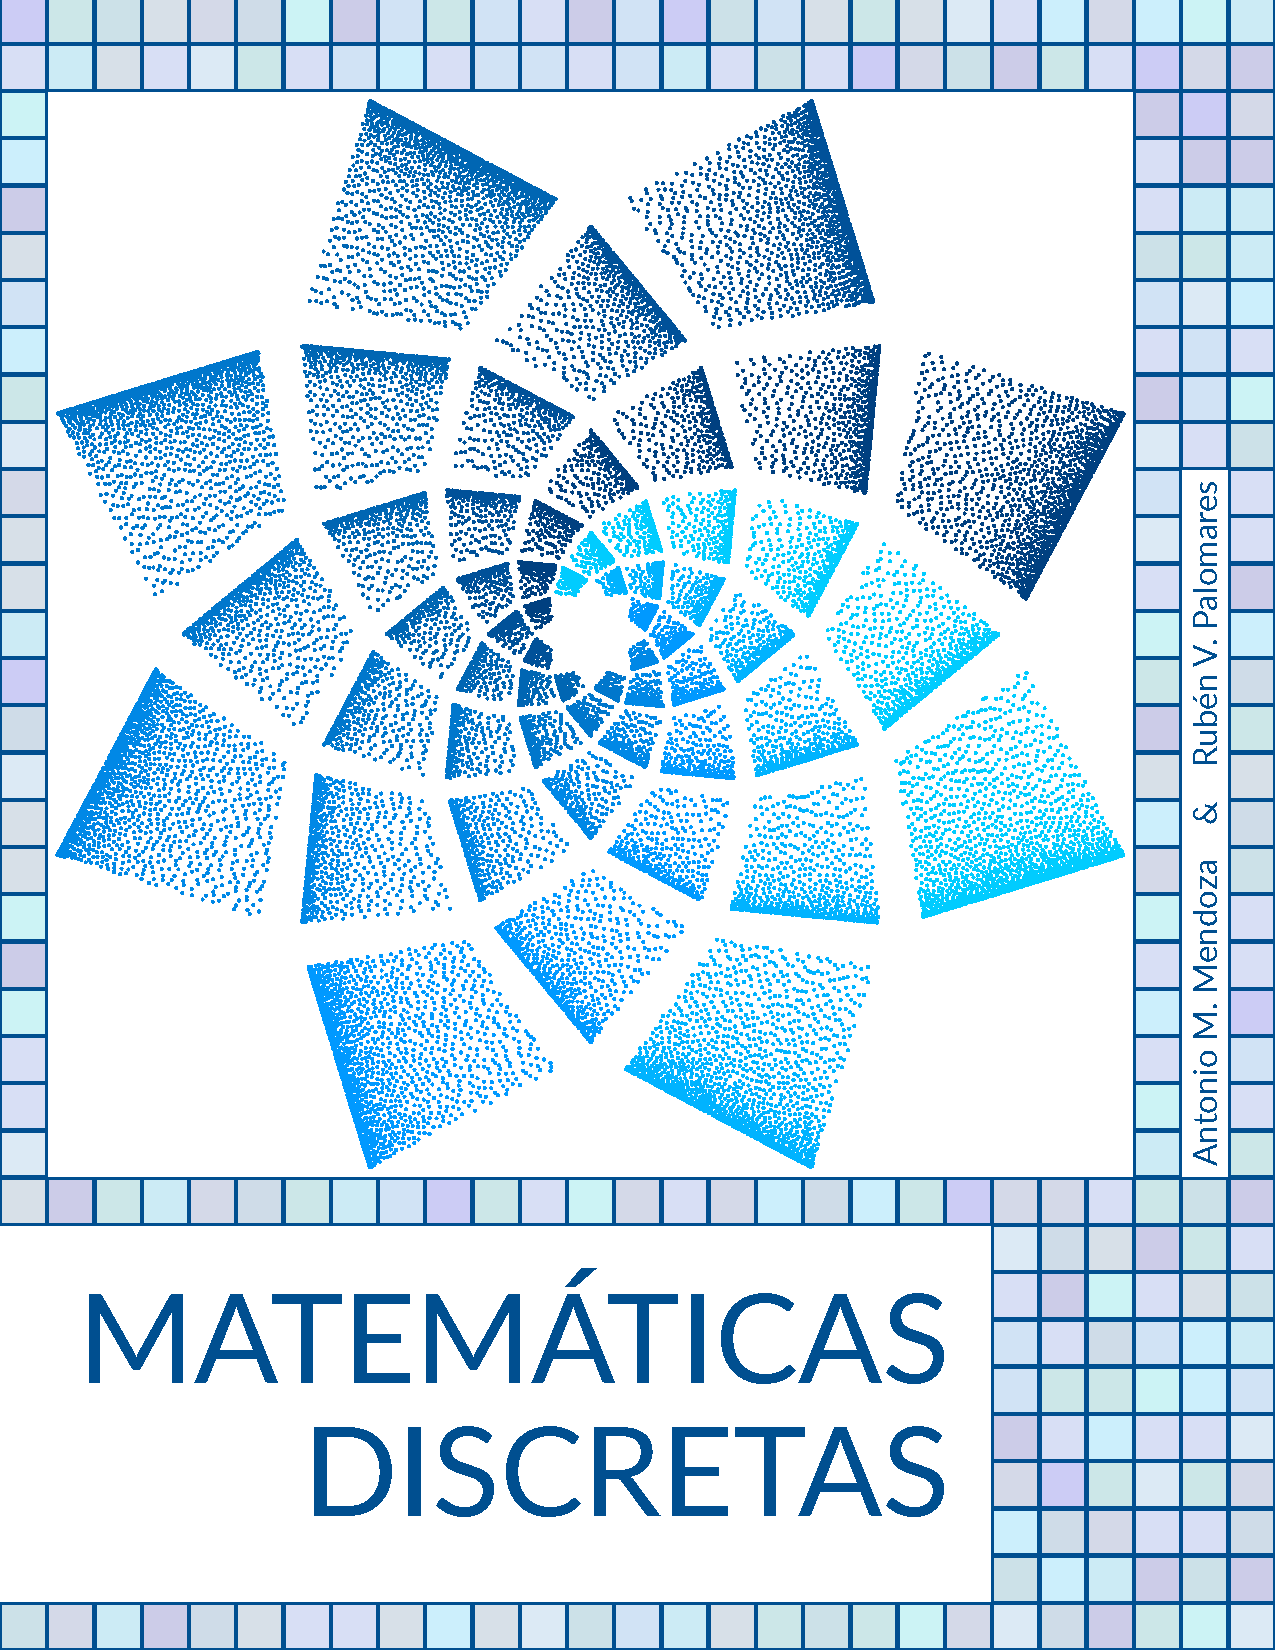
\includepdf[pages=-]{Portada_de_colores.pdf}

\newpage 

\begin{tikzpicture}[remember picture,overlay]%
      \coordinate (A) at ($(current page.north)!.4!(current page.north east)$);
      \coordinate (B) at (current page.east);
      \coordinate (C) at (current page.north east);

      \filldraw[jblueleft] (A) -- (B) -- (C) -- cycle;
\end{tikzpicture}

\,
\vspace{3cm}
\begin{center}
\scalebox{3}{\textbf{\color{jblueleft}MATEMÁTICAS DISCRETAS}}\\
\,
\,\\
\scalebox{2}{\textbf{\color{jblueleft}Una introducción con aplicaciones}}\\
\,\\
\,\\
\scalebox{1.3}{\textbf{\color{jblueleft} Rubén Ramón Vargas Palomares}}\\
\,\\
Profesor de matemáticas de la ESFM\\
\vspace{2cm}
\begin{center}
      \begin{tikzpicture}
            \node at (current page.center) {
\includegraphics[width=0.5\textwidth]{Images/IPNAZUL.pdf}}; % Logo de institución
      \end{tikzpicture}
\end{center}
\vfill
México, 2023
\end{center}

\newpage
\,

\newpage

~\vfill\hfill\begin{minipage}[l]{0.55\textwidth}
     \itshape Quiero expresar mi agradecimiento al Lic. Rubén Ramón Vargas Palomares, quien aparte de haber sido mi profesor, me permitió recopilar el presente trabajo.
\end{minipage}

\newpage
\,

\chapterimage{blue20.jpeg} % Imagen de encabezado de capítulo
\chapterspaceabove{6.75cm} % Espacio en blanco desde la parte superior de la página hasta el título del capítulo en las páginas del capítulo
\chapterspacebelow{7.25cm} % Cantidad de espacio en blanco vertical desde el margen superior hasta el comienzo del texto en las páginas de los capítulos

\renewcommand{\contentsname}{CONTENIDO}
\tableofcontents
\label{toc-contents}

%\listoffigures

\newpage

\chapterimage{blue21.jpeg} % Imagen de encabezado de capítulo
\chapterspaceabove{6.75cm} % Espacio en blanco desde la parte superior de la página hasta el título del capítulo en las páginas del capítulo
\chapterspacebelow{7.25cm} % Cantidad de espacio en blanco vertical desde el margen superior hasta el comienzo del texto en las páginas de los capítulos

%------------------------------------------------

\chapter*{PREFACIO}

Se recalca que esta obra son notas del curso de Matemáticas Discretas, por lo que es probable que exista algún error ortográfico o matemático. Se recomienda consultar la bibliografía proporcionada al final de este trabajo. La presente obra consta de todo el contenido que adjudicó el Lic. Rubén Ramón Vargas Palomares, quien imparte clases en la Escuela Superior de Física y Matemáticas (ESFM) en el Instituto Politécnico Nacional (IPN). Hice el mayor esfuerzo en estructurar el libro a base de proposiciones, ejercicios, notas, etc.; y se agregaron y modificaron algunas definiciones, a fin de lograr una mayor comprensión sin llegar a tener alguna ambigüedad.\\


Cada capítulo contiene varios ejercicios y demostraciones. Estos son de diversos tipos y pueden ayudar a tener una mejor comprensión del tema. Cabe mencionar que este libro fue mecanografiado por Marco Antonio Molina Mendoza, estudiante de la Escuela Superior de Física y Matemáticas. Si lo deseas o lo requieres, puedes imprimir esta obra, eres libre de hacerlo y no necesitas autorización. Cualquier mención a esta obra es apreciada, pero no requerida. Se sigue trabajando para corregir errores y/o mejorar este trabajo, por lo que está en constante cambio. Se recomienda entrar en  \href{https://linktr.ee/biblioteca_esfm}{\textbf{\color{jblueleft}Biblioteca ESFM}} para encontrar la versión más actualizada.

\begin{center}
    \begin{tikzpicture}
        \node[fill=white] at (0,0) {\qrcode[hyperlink, height=3cm]{https://linktr.ee/biblioteca_esfm}};
    \end{tikzpicture}
\end{center}

Algunos cambios han sido resultado de los comentarios de mis amigos y estudiantes de la Escuela Superior de Física y Matemáticas. Estas son algunas de las muchas mejoras que se han incorporado en esta edición.
\begin{itemize}
    \item Aspecto estético mejorado: He trabajo arduamente para crear un diseño atractivo y cómodo a la vista. Nuevas fuentes, estilos y esquemas de color se han utilizado para mejorar la legibilidad y facilitar la asimilación de los conceptos.
    \item Errores ortográficos y matemáticos corregidos: He realizado una revisión minuciosa para garantizar la precisión en todos los aspectos del contenido. Los errores ortográficos y matemáticos se han corregido para ofrecer una experiencia de aprendizaje fluida y confiable.
    \item Imágenes actualizadas: He renovado todas las imágenes y gráficos del libro para asegurarme de que sean claros, informativos y visualmente atractivos. Las nuevas ilustraciones ayudarán a comprender mejor los conceptos y aplicaciones de la matemática discreta en el mundo real.
    \item Ejemplos adicionales y ejercicios prácticos: He añadido más ejemplos paso a paso y problemas resueltos para reforzar el entendimiento de los temas discutidos.
    %\item Recuadros de resumen y notas destacadas: Hemos agregado recuadros de resumen al final de cada sección para recapitular los puntos clave. Además, hemos incluido notas destacadas para enfatizar conceptos importantes y recordatorios útiles a lo largo del libro.
\end{itemize}

Con una presentación clara y concisa de los temas, busco fomentar la apreciación de la belleza y utilidad de esta rama de las matemáticas. Se aspira a que los lectores adquieran las habilidades y conocimientos necesarios para resolver problemas complejos y se sientan motivados a explorar aplicaciones más avanzadas de la matemática discreta en su futuro académico y profesional.\\


Este libro (en PDF) está diseñado en tres grandes enlaces
\begin{itemize}
    \item Números de páginas: Lo podrás encontrar en la parte superior derecha e izquierda dependiendo si es una página par o impar; al dar clic te llevará al índice de este libro.
    \item Nombres de secciones en el encabezado: Lo podrás encontrar en la parte superior derecha de cada página impar; al dar clic te llevará al comienzo de dicha sección.
    \item Nombres de capítulos en el encabezado: Lo podrás encontrar en la parte superior izquierda de cada página par; al dar clic te llevará al comienzo de dicho capítulo.
\end{itemize}

Esta obra se hizo gracias a \textbf{\textsf{\color{jblueleft}El Libro Azul}} (tercera versión), una plantilla hecha en \LaTeX\ que podrás encontrar en:
\begin{center}
    \color{jblueleft}
    \underline{\url{https://drive.google.com/drive/folders/1_zVKfxadoDAeL0Yrz9_RzXQuhQfiJ8ig}}
\end{center}
\cczero\ Esta plantilla se publica en el dominio público utilizando el código CC0. En la medida de lo posible bajo la ley, yo renunció a todos los derechos de autor y derechos relacionados o conexos a este trabajo.\\


Además, las imágenes que se presentan en este libro están hechas con el paquete \texttt{Tikz}, una herramienta para la producción de gráficos vectoriales. Dichas imágenes son de elaboración propia; y de igual manera, son de dominio público.

\vfill

\begin{center}
    \begin{tikzpicture}
        \node at (0,0) {
\includegraphics[width=3.5cm]{Images/ESCUDO_ESFM.pdf}};
        \node at (6,0) {
\includegraphics[width=3.5cm]{Images/LOGO.pdf}};
    \end{tikzpicture}
\end{center}

\part[\vspace{-0.13cm}FUNDAMENTOS DE LA MATEMÁTICA DISCRETA]{FUNDAMENTOS DE LA MATEMÁTICA DISCRETA}

\pagestyle{fancy}

\chapterimage{blue22.jpeg} % Imagen de encabezado de capítulo
\chapterspaceabove{6.75cm} % Espacio en blanco desde la parte superior de la página hasta el título del capítulo en las páginas del capítulo
\chapterspacebelow{7.25cm} % Cantidad de espacio en blanco vertical desde el margen superior hasta el comienzo del texto en las páginas de los capítulos

%------------------------------------------------

\chapter{FUNDAMENTOS DE LÓGICA}\label{chap:1}

En el contexto de Matemáticas Discretas, la lógica es el estudio formal de los principios y reglas que gobiernan el razonamiento válido y la inferencia. Se centra en el análisis de cómo se pueden combinar proposiciones o afirmaciones para obtener conclusiones válidas a partir de ellas. La lógica se utiliza para estructurar el pensamiento y garantizar que nuestras deducciones sean sólidas y coherentes.

En Matemáticas Discretas, la lógica es esencial para establecer una base sólida para la argumentación y la resolución de problemas. Hay dos aspectos clave de la lógica que se estudian:

\begin{enumerate}
    \item Lógica Proposicional: También conocida como lógica de enunciados, se centra en el análisis de proposiciones individuales y cómo se pueden combinar utilizando conectivos lógicos como la negación, conjunción, disyunción, implicación y bicondicional. La lógica proposicional se utiliza para construir expresiones lógicas complejas y analizar su valor de verdad bajo diferentes combinaciones de valores de verdad para las proposiciones individuales.
    \item Lógica de Predicados: Esta rama de la lógica permite expresar relaciones y propiedades entre objetos utilizando cuantificadores como \emph{para todo} ($\forall$) y \emph{existe} ($\exists$). La lógica de predicados es más expresiva y permite hablar sobre conjuntos de objetos y sus propiedades en un nivel más profundo.
\end{enumerate}

En clase, los estudiantes de Matemáticas Discretas aprenden a construir tablas de verdad para evaluar expresiones lógicas, aplicar reglas y propiedades de la lógica para simplificar y demostrar proposiciones, y utilizar la lógica para establecer argumentos válidos en diversas situaciones. En última instancia, el estudio de la lógica en Matemáticas Discretas proporciona habilidades fundamentales para resolver problemas de manera estructurada, identificar errores en el razonamiento y construir argumentos sólidos basados en reglas bien definidas. Estas habilidades son esenciales en la informática, las matemáticas y muchos otros campos donde se requiere análisis lógico y razonamiento riguroso.


\section{Proposiciones}

Con el estudio de la Lógica se persigue llegar a ser preciso y cuidadoso. La Lógica tiene un lenguaje exacto. Pero aunque así sea, vamos a intentar construir un vocabulario para este lenguaje preciso utilizando el lenguaje cotidiano algunas veces un tanto confuso. Es necesario redactar un conjunto de reglas que sean perfectamente claras y definidas y que estén libres de las vaguedades que pueden hallarse en nuestro lenguaje corriente. Para realizar este trabajo se utilizarán proposiciones en lengua castellana, de la misma manera que se usa la lengua castellana para explicar las reglas precisas de un juego a alguien que no ha jugado a ese juego. Por supuesto, la lógica es algo más que un juego. Puede ayudarnos a aprender una forma de razonar que es exacta y a la vez muy útil. En el desarollo de cualquer teoría matemática se hacen afirmaciones en forma de frases, las cuales se denominan \emph{enunciados} o \emph{proposiciones} que pueden ser falsos o verdaderos.

\begin{myexamples}
    \begin{enumerate}
        \item El número $\pi$ es entero.
        \item La división entre cero no está definida.
        \item 13 es un número primo.
    \end{enumerate}
\end{myexamples}


\section{Simbolización de proposiciones}

Generalmente se cree que las proposiciones son proposiciones cortas, pero también algunas de las proposiciones del lenguaje corriente son largas, resultando por ello pesadas y de difícil manejo. En lógica se afronta este problema utilizando símbolos en lugar de las proposiciones completas. Los símbolos que usaremos en lógica para representar proposiciones, son letras mayúsculas tales como $P$, $Q$, $R$, $S$, $A$, y $B$.

\begin{myexamples}
    Tomando los ejemplos anteriores
    \begin{enumerate}
        \item $P=\text{El número } \pi \text{ es entero.}$
        \item $Q=\text{La división entre cero no está definida.}$
        \item $R=13 \text{ es un número primo.}$
    \end{enumerate}
\end{myexamples}


\section{Términos de enlace o conectivos}

En lógica, los conectivos son términos que se utilizan para combinar proposiciones simples y crear proposiciones más complejas. Estos conectivos permiten construir expresiones lógicas al conectar declaraciones individuales de diversas maneras. Las proposiciones primitivas no pueden descomponerse en partes más simples y son utilizadas con los conectivos lógicos para formar enunciados compuestos. Algunos ejemplos comunes de conectivos incluyen:

\begin{enumerate}
	\item Negación ($\neg$): Este conectivo cambia el valor de verdad de una proposición. Si una proposición es verdadera, su negación será falsa, y viceversa.
	\item Conjunción ($\land$): Este conectivo se utiliza para combinar dos proposiciones, y la proposición resultante es verdadera solo si ambas proposiciones individuales son verdaderas.
	\item Disyunción ($\lor$): La disyunción se utiliza para combinar dos proposiciones, y la proposición resultante es verdadera si al menos una de las proposiciones individuales es verdadera.
    \item Disyunción exclusiva ($\veebar$): La disyunción exclusiva se utiliza para combinar dos proposiciones en donde la proposición resultante es verdadera si exactamente una de las dos proposiciones individuales es verdadera, mientras que si ambas son verdaderas o ambas son falsas, la proposición resultante es falsa.
	\item Implicación ($\rightarrow$): Este conectivo establece una relación condicional entre dos proposiciones. La proposición “$P \rightarrow Q$” se lee como “Si $P$, entonces $Q$”. Es falsa solo cuando $P$ es verdadera y $Q$ es falsa.
	\item Equivalencia ($\leftrightarrow$): La equivalencia se utiliza para expresar que dos proposiciones son verdaderas o falsas al mismo tiempo. La proposición “$P \leftrightarrow Q$” se lee como “Si $P$ entonces $Q$, si $Q$ entonces $P$”.
\end{enumerate}

Estos conectivos son fundamentales para construir expresiones lógicas más complejas y realizar razonamientos basados en reglas lógicas.

\begin{myexample}
    Tomando las proposiciones $Q$ y $R$ del ejemplo anterior, podemos formar lo siguiente:
    \begin{center}
        (La división entre cero no está definida) \textcolor{jblueleft}{y} (13 es un número primo)

        (La división entre cero no está definida) \textcolor{jblueleft}{o} (13 es un número primo)
    \end{center}
\end{myexample}

\begin{importante}
    Algunos libros y/o autores denotan la negación de una proposición $P$ con $\overline{P}$.
\end{importante}


\section{Tablas de verdad}

Las tablas de verdad son especialmente útiles para analizar y comprender el comportamiento de conectivos lógicos y expresiones complejas. Ayudan a visualizar cómo cambian los valores de verdad a medida que las proposiciones individuales varían y cómo esos cambios afectan el valor de verdad de la expresión global.

Las tablas que mostraremos a continuación, usaran al 0 para decir que la proposición es falsa y el 1 para decir que la proposición es verdadera.

\begin{center}
\begin{minipage}[c]{0.2\textwidth}
    \begin{center}
        \begin{NiceTabular}[hvlines-except-borders,rules={color=white,width=1pt}]{cc}
        \CodeBefore
        \rowcolor{jblueleft!80}{1}
        \rowcolors{2}{DodgerBlue3!40}{jblueinner}
        \Body
        \RowStyle[color=white]{}
            $P$ & $\neg P$ \\
            0 & 1 \\
            1 & 0 \\ 
        \end{NiceTabular}
        \captionof{table}{~}
    \end{center}
\end{minipage}
\hspace{1cm}
\begin{minipage}[c]{0.6\textwidth}
    \begin{center}
        \begin{NiceTabular}[hvlines-except-borders,rules={color=white,width=1pt}]{ccccccc}
        \CodeBefore
        \rowcolor{jblueleft!80}{1}
        \rowcolors{2}{DodgerBlue3!40}{jblueinner}
        \Body
        \RowStyle[color=white]{}
            $P$ & $Q$ & $P \land Q$ & $P \lor Q$ & $P \veebar Q$ & $P \rightarrow Q$ & $P \leftrightarrow Q$ \\
            0 & 0 & 0 & 0 & 0 & 1 & 1 \\
            0 & 1 & 0 & 1 & 1 & 1 & 0 \\ 
            1 & 0 & 0 & 1 & 1 & 0 & 0 \\
            1 & 1 & 1 & 1 & 0 & 1 & 1 \\ 
        \end{NiceTabular}
        \captionof{table}{~}
    \end{center}
\end{minipage}
\end{center}

Si agregamos una proposición $R$, tenemos la siguiente tabla de verdad:

\begin{center}
    \begin{NiceTabular}[hvlines-except-borders,rules={color=white,width=1pt}]{cccccc}
        \CodeBefore
        \rowcolor{jblueleft!80}{1}
        \rowcolors{2}{DodgerBlue3!40}{jblueinner}
        \Body
        \RowStyle[color=white]{}
        $P$ & $Q$ & $R$ & $\neg R$ & $R \rightarrow P$ & $Q \land \left( \neg R \rightarrow P \right)$ \\ 
        0 & 0 & 0 & 1 & 0 & 0 \\
        0 & 0 & 1 & 0 & 1 & 0 \\ 
        0 & 1 & 0 & 1 & 0 & 0 \\
        0 & 1 & 1 & 0 & 1 & 1 \\
        1 & 0 & 0 & 1 & 1 & 0 \\
        1 & 0 & 1 & 0 & 1 & 0 \\
        1 & 1 & 0 & 1 & 1 & 1 \\
        1 & 1 & 1 & 0 & 1 & 1
    \end{NiceTabular}
    \captionof{table}{~}
\end{center}

\begin{definicion}{}{}
    Sean $S_1$ y $S_2$ dos proposiciones. Se dice que $S_1$ y $S_2$ son lógicamente equivalentes cuando sus tablas de verdad tienen los mismos valores y lo denotaremos como $S_1 \Leftrightarrow S_2$.
\end{definicion}

\begin{myexample}
    De las siguientes tablas de verdad \\

    
    \hspace{-1cm}
    %\begin{center}
        \begin{minipage}[c]{0.4\textwidth}
            \begin{center}
                \begin{NiceTabular}[hvlines-except-borders,rules={color=white,width=1pt}]{ccccc}
                \CodeBefore
                \rowcolor{jblueleft!80}{1}
                \rowcolors{2}{DodgerBlue3!40}{jblueinner}
                \Body
                \RowStyle[color=white]{}
                    $P$ & $Q$ & $\overline{P}$ & $\overline{P} \lor Q$ & $P \rightarrow Q$ \\
                    0 & 0 & 1 & 1 & 1 \\
                    0 & 1 & 1 & 1 & 1 \\
                    1 & 0 & 0 & 0 & 0 \\
                    1 & 1 & 0 & 1 & 1
                \end{NiceTabular}
                \captionof{table}{~}
            \end{center}
        \end{minipage}
        \hspace{-0.5cm}
        \begin{minipage}[c]{0.60\textwidth}
            \begin{center}
                \begin{NiceTabular}[hvlines-except-borders,rules={color=white,width=1pt}]{cccccc}
                \CodeBefore
                \rowcolor{jblueleft!80}{1}
                \rowcolors{2}{DodgerBlue3!40}{jblueinner}
                \Body
                \RowStyle[color=white]{}
                    $P$ & $Q$ & $P \rightarrow Q$ & $Q \rightarrow P$ & $(P \rightarrow Q) \land (Q \rightarrow P)$ & $P \leftrightarrow Q$ \\
                    0 & 0 & 1 & 1 & 1 & 1 \\
                    0 & 1 & 1 & 0 & 0 & 0 \\
                    1 & 0 & 0 & 1 & 0 & 0 \\
                    1 & 1 & 1 & 1 & 1 & 1
                \end{NiceTabular}
                \captionof{table}{~}
            \end{center}
        \end{minipage}
    %\end{center}

    \,\\
    \noindent
    se obtienen estas equivalencias lógicas
    \begin{enumerate}
        \item $(P \leftrightarrow Q) \Leftrightarrow \left[ (P \rightarrow Q) \land (Q \rightarrow P) \right]$.
        \item $(P \leftrightarrow Q) \Leftrightarrow \left[ \left( \overline{P} \lor Q \right) \land \left( \overline{Q} \lor P \right) \right]$.
    \end{enumerate}
\end{myexample}

\begin{myexample}
    De la siguiente tabla de verdad
    
    \begin{center}
        \begin{NiceTabular}[hvlines-except-borders,rules={color=white,width=1pt}]{ccccccc}
        \CodeBefore
        \rowcolor{jblueleft!80}{1}
        \rowcolors{2}{DodgerBlue3!40}{jblueinner}
        \Body
        \RowStyle[color=white]{}
            $P$ & $Q$ & $P \veebar Q$ & $P \lor Q$ & $P \land Q$ & $\overline{P \land Q}$ & $(P \lor Q) \land \overline{(P \land Q)}$ \\
            0 & 0 & 0 & 0 & 0 & 1 & 0 \\
            0 & 1 & 1 & 1 & 0 & 1 & 1 \\
            1 & 0 & 1 & 1 & 0 & 1 & 1 \\
            1 & 1 & 0 & 1 & 1 & 0 & 0
        \end{NiceTabular}
        \captionof{table}{~}
    \end{center}
    se obtiene la equivalencia lógica
    $$(P \veebar Q) \Leftrightarrow (P \lor Q) \land \overline{(P \land Q)}.$$
\end{myexample}

\begin{obs}{}{}
    Al considerar la siguiente tabla de verdad
    \begin{center}
        \begin{NiceTabular}[hvlines-except-borders,rules={color=white,width=1pt}]{ccccccc}
        \CodeBefore
        \rowcolor{jblueleft!80}{1}
        \rowcolors{2}{DodgerBlue3!40}{jblueinner}
        \Body
        \RowStyle[color=white]{}
            $P$ & $\overline{P}$ & $Q$ & $P \lor Q$ & $P \rightarrow (P \lor Q)$ & $\overline{P} \land Q$ & $P \land \left( \overline{P} \land Q \right)$ \\
            0 & 1 & 0 & 0 & 1 & 0 & 0 \\
            0 & 1 & 1 & 1 & 1 & 1 & 0 \\
            1 & 0 & 0 & 1 & 1 & 0 & 0 \\
            1 & 0 & 1 & 1 & 1 & 0 & 0 
        \end{NiceTabular}
        \captionof{table}{~}
    \end{center}
    se deduce que el enunciado $P \rightarrow (P \lor Q)$ siempre es verdadero, pero el enunciado $P \land \left( \overline{P} \land Q \right)$ siempre es falso.
\end{obs}

\newpage

\begin{definicion}{}{}
    Una proposición que siempre es verdadera se denomina tautología y la denotaremos por $T_0$.
\end{definicion}

\begin{definicion}{}{}
    Una proposición que siempre es falsa se denomina contradicción y la denotaremos por $F_0$.
\end{definicion}

\begin{definicion}{}{}
    Si para las proposiciones $S_1$ y $S_2$ resulta que $S_1 \leftrightarrow S_2$ es una tautología, entonces $S_1$ y $S_2$ deben tener los mismos valores en la tabla de verdad, de modo que se cumple la equivalencia lógica $S_1 \Leftrightarrow S_2$.
\end{definicion}

\begin{definicion}{}{}
    Si para las proposiciones $S_1$ y $S_2$ resulta que $S_1 \rightarrow S_2$ es una tautología, se dice que $S_1$ implica lógicamente a $S_2$ y lo denotaremos como $S_1 \Rightarrow S_2$.
\end{definicion}

\section{Reglas de inferencia}

Las reglas de inferencia son un conjunto de principios lógicos que se utilizan para justificar o validar argumentos y razonamientos en lógica formal. Estas reglas proporcionan un marco estructurado y coherente para determinar si una conclusión dada puede deducirse lógicamente a partir de un conjunto de premisas o proposiciones dadas. En esencia, las reglas de inferencia ayudan a determinar si un argumento es válido o no.\\


El propósito fundamental de las reglas de inferencia es permitirnos llevar a cabo inferencias lógicas válidas, lo que significa que si todas las premisas son verdaderas, entonces la conclusión derivada también debe ser verdadera. Esto es crucial en la lógica y el razonamiento formal, ya que garantiza que nuestras conclusiones estén respaldadas por una base lógica sólida.\\


Estas reglas son esenciales en una variedad de campos, como la filosofía, las matemáticas, la ciencia de la computación y la inteligencia artificial, donde se requiere el razonamiento lógico para resolver problemas y tomar decisiones informadas. Además, las reglas de inferencia se utilizan en la construcción de pruebas matemáticas y en la demostración de teoremas, lo que las convierte en un componente fundamental de la metodología matemática rigurosa.\\


Algunos ejemplos comunes de reglas de inferencia en la lógica proposicional incluyen:

\begin{enumerate}
    \item Modus Ponens: Si se tiene una proposición “$P \rightarrow Q$” (si $P$, entonces $Q$) y también se sabe que “$P$” es verdadera, entonces se puede inferir que “$Q$” también es verdadera.
    \item Modus Tollens: Si se tiene una proposición “$P \rightarrow Q$” y se sabe que “$Q$” es falsa, entonces se puede inferir que “$P$” también es falsa.
    \item Silogismo: Si se tiene una proposición “$P \lor Q$” ($P$ o $Q$) y se sabe que “$P$” es verdadera, se puede inferir que “$Q$” es falsa.
\end{enumerate}

Estas son solo algunas de las muchas reglas de inferencia que existen en la lógica. Las reglas de inferencia ayudan a formalizar el proceso de razonamiento y garantizan que las conclusiones extraídas sean válidas y consistentes según las reglas lógicas establecidas.

\newpage

\section{Leyes de la lógica}

Las leyes de la lógica son principios fundamentales que rigen el razonamiento válido y la inferencia en el ámbito de la lógica formal. Estas leyes establecen reglas y relaciones entre proposiciones y conectivos lógicos, y son esenciales para garantizar que los argumentos sean coherentes y las deducciones sean sólidas. Las leyes de la lógica se derivan de la estructura misma de las proposiciones y los conectivos, y proporcionan la base para el análisis lógico y la construcción de argumentos válidos.\\


Con los conceptos de equivalencia lógica, tautología y contradicción, enunciamos la siguiente tabla de leyes de la lógica:

\begin{center}
    \begin{NiceTabular}[hvlines-except-borders,rules={color=white,width=1pt}]{ll}
        \CodeBefore
        %\rowcolor{jblueleft!80}{1}
        \rowcolors{1}{DodgerBlue3!40}{jblueinner}
        \Body
        %\RowStyle[color=white]{}
            Ley de la doble negación & $\begin{array}{l}\overline{\overline{P}} \Leftrightarrow P \end{array}$ \\
            Leyes de De Morgan & $\begin{array}{l}
                \overline{P \lor Q} \Leftrightarrow \overline{P} \land \overline{Q} \\
                \overline{P \land Q} \Leftrightarrow \overline{P} \lor \overline{Q}
            \end{array}$ \\
            Leyes conmutativas & $\begin{array}{l}
                P \lor Q \Leftrightarrow Q \lor P \\
                P \land Q \Leftrightarrow Q \land P
            \end{array}$ \\
            Leyes asociativas & $\begin{array}{l}
                P \lor (Q \lor R) \Leftrightarrow (P \lor Q) \lor R \\
                P \land (Q \land R) \Leftrightarrow (P \land Q) \land R
            \end{array}$ \\
            Leyes distributivas & $\begin{array}{l}
                P \lor (Q \land R) \Leftrightarrow (P \lor Q) \land (P \lor R) \\
                P \land (Q \lor R) \Leftrightarrow (P \land Q) \lor (P \land R)
            \end{array}$ \\
            Leyes idempotentes & $\begin{array}{l}
                P \lor P \Leftrightarrow P \\
                P \lor P \Leftrightarrow P
            \end{array}$ \\
            Leyes del inverso & $\begin{array}{l}
                P \lor F_0 \Leftrightarrow P \\
                P \land T_0 \Leftrightarrow P
            \end{array}$ \\
            Leyes de dominación & $\begin{array}{l}
                P \lor T_0 \Leftrightarrow T_0 \\
                P \land F_0 \Leftrightarrow F_0
            \end{array}$ \\
            Leyes de absorción & $\begin{array}{l}
                P \lor (P \land Q) \Leftrightarrow P \\
                P \land (P \lor Q) \Leftrightarrow P
            \end{array}$
    \end{NiceTabular}
    \captionof{table}{Leyes de la lógica}\label{table1}
\end{center}

\chapterimage{blue14.jpeg} % Imagen de encabezado de capítulo
\chapterspaceabove{6.75cm} % Espacio en blanco desde la parte superior de la página hasta el título del capítulo en las páginas del capítulo
\chapterspacebelow{7.25cm} % Cantidad de espacio en blanco vertical desde el margen superior hasta el comienzo del texto en las páginas de los capítulos

%------------------------------------------------

\chapter{TÉCNICAS DE CONTEO}\label{chap:2}


En el emocionante mundo de las Matemáticas Discretas, existen herramientas y métodos que nos permiten abordar problemas complejos de manera estructurada y precisa. Uno de los aspectos más fascinantes de este campo es la aplicación de las técnicas de conteo, una habilidad esencial para contar y cuantificar conjuntos finitos de objetos. Estas técnicas nos brindan la capacidad de analizar y resolver problemas relacionados con la cantidad de formas en que ciertos eventos pueden ocurrir, sin necesidad de enumerar cada posibilidad individualmente.

El capítulo que exploraremos a continuación se sumerge en el intrigante mundo de las técnicas de conteo en Matemáticas Discretas. Aquí descubriremos cómo contar y calcular de manera eficiente, evitando la repetición de casos y garantizando que no pasemos por alto ninguna posibilidad. Desde contar permutaciones y combinaciones hasta abordar problemas de distribución y partición, estas técnicas no solo son fundamentales en matemáticas, sino que también tienen aplicaciones en áreas como la informática, la estadística y la teoría de la probabilidad.\\



Las técnicas de conteo son más que simples procedimientos matemáticos; son herramientas poderosas que nos ayudan a desentrañar la complejidad de problemas aparentemente intrincados. A través de las técnicas de conteo en Matemáticas Discretas, descubriremos cómo contar, calcular y abordar desafíos con una claridad renovada y una habilidad recién adquirida.


\section{Reglas de la suma y el producto}

\begin{tcolorbox}[
      theorem style=change break,
      enhanced,
      breakable,
      boxrule=0pt,
      frame hidden,
      borderline west={3pt}{0pt}{jblueleft},
      colback=jblueinner,
      coltitle=jblueleft,
      attach title to upper={\ },
      sharp corners,
      title={Regla de la suma:},
      fonttitle=\bfseries,
      fontupper=\normalsize
]
    Si una primera tarea puede realizarse de $m$ formas, mientras que una segunda tarea puede realizarse de $n$ formas, y no es posible realizar ambas tareas de manera simultánea, entonces, para llevar a cabo cualquiera de ellas pueden utilizarse cualquiera de $m + n$ formas.
\end{tcolorbox}

\begin{myexample}
    La biblioteca de una universidad tiene 40 libros de texto de sociología y 50 de antropología. Por la regla de la suma, un estudiante de esta universidad puede elegir entre $40 + 50 = 90$ libros de texto para aprender acerca de alguno de estos dos temas.
\end{myexample}

\newpage 

\begin{tcolorbox}[
      theorem style=change break,
      enhanced,
      breakable,
      boxrule=0pt,
      frame hidden,
      borderline west={3pt}{0pt}{jblueleft},
      colback=jblueinner,
      coltitle=jblueleft,
      attach title to upper={\ },
      sharp corners,
      title={Regla del producto:},
      fonttitle=\bfseries,
      fontupper=\normalsize
]
    Si un procedimiento se puede descomponer en las etapas primera y segunda, y si existen $m$ resultados posibles de la primera etapa y si, para cada uno de estos resultados, existen $n$ resultados posibles para la segunda etapa, entonces el procedimiento total se puede realizar, en el orden dado, de $mn$ formas.
\end{tcolorbox}

\begin{importante}{}{}
    A la regla del producto también se le conoce como el \textbf{principio de elección}.
\end{importante}

\begin{myexample}
    En una oficina se solicita una secretaria y un supervisor. Si hay 5 candidatos para el puesto de secretaria y 5 candidatos para el puesto de supervisor, entonces por el principio del producto es posible asignar la pareja de puestos vacantes de $(5)(5) = 25$ formas distintas.
\end{myexample}

\begin{obs}{}{}
    Si asignamos a cada secretaria y supervisor con una letra respectivamente, es decir,
    \begin{center}
        \begin{tabular}{lccccc}
            Secretaria & a & b & c & d & e \\
            Supervisor & f & g & h & i & j
        \end{tabular}
    \end{center}
    Podemos mostrar las posibilidades del ejemplo anterior con un diagrama de árbol como sigue:\\
    
    \Tree[.{Número de vacantes} [.a [.f ] [.g ] [.h ] [.i ] [.j ] ] [.b [.f ] [.g ] [.h ] [.i ] [.j ] ] [.c [.f ] [.g ] [.h ] [.i ] [.j ] ] [.d [.f ] [.g ] [.h ] [.i ] [.j ] ] [.e [.f ] [.g ] [.h ] [.i ] [.j ] ] ]
\end{obs}

\section{Permutaciones}

\begin{definicion}{}{}
    Sea $n \in \ZZ[+]$. Definimos el \textbf{factorial} de $n$, denotado por $n!$, como
    $$n! = (n)(n-1)(n-2) \cdots (3)(2)(1).$$
\end{definicion}

\begin{myexample}
    Usando la definición anterior, si $n = 4$, entonces
    \begin{align*}
        4! & = (4)(4-1)(4-2)(4-3) \\
        & = (4)(3)(2)(1) \\
        & = 24.
    \end{align*}
\end{myexample}

\newpage

\begin{importante}{}{}
    Las permutaciones de objetos se pueden definir como las \textbf{ordenaciones} de estos mismos.
\end{importante}

\begin{myexample}
    Se quieren ordenar 5 libros distintos en un estante:
    \begin{center}
        \begin{tikzpicture}
            \draw[jblueleft] (0,0) rectangle (1,3);
            \draw[jblueleft] (1,0) rectangle (2,2);
            \draw[jblueleft] (2,0) rectangle (3,1.5);
            \draw[jblueleft] (3,0) rectangle (4,2.5);
            \draw[jblueleft] (4,0) rectangle (5,3);

            \node[jblueleft] at (0.5,1.5) {a};
            \node[jblueleft] at (1.5,1) {b};
            \node[jblueleft] at (2.5,0.75) {c};
            \node[jblueleft] at (3.5,1.25) {d};
            \node[jblueleft] at (4.5,1.5) {e};
        \end{tikzpicture}
    \end{center}
    Algunas ordenaciones son
    \begin{center}
        \begin{tabular}{ccccc}
            a & b & c & d & e \\
            c & a & b & c & d \\
            d & e & a & b & c
        \end{tabular}
    \end{center}
    Notemos que al aplicar el principio del producto, obtenemos
    \begin{align*}
        5! & = (5)(4)(3)(2)(1) \\
        & = 120 \text{ ordenaciones diferentes.}
    \end{align*}
\end{myexample}

\begin{notation*}{}
    Denotaremos al número de permutaciones como
    $$P(n, \, n) = {}_nP_n = n!.$$
\end{notation*}

\begin{myexample}
    A partir de un grupo de 10 personas se van a seleccionar 5 de ellas para formarlas en una fila de 5 sillas para fotografiarlas. ¿Cuántas permutaciones (ordenaciones) diferentes se pueden hacer?\\
    \newline
    \textbf{\color{jblueleft}Solución:} Si asignamos a cada persona una letra, es decir
    \begin{center}
        \begin{tabular}{ccccccccccc}
            Personas & a & b & c & d & e & f & g & h & i & j
        \end{tabular}
    \end{center}
    obtenemos
    \begin{center}
        \begin{tabular}{cccccccccc}
            10 & & 9 & & 8 & & 7 & & 6 \\
            primera & & segunda & & tercera & & cuarta & & quinta \\
            posición & & posición & & posición & & posición & & posición
        \end{tabular}
    \end{center}
    es decir,
    \begin{align*}
        P(10, \, 5) & = (10)(9)(8)(7)(10-5+1) \\ 
        & = 30 \, 240 \text{ ordenaciones.}
    \end{align*}
    Si se utiliza la notación factorial:
    \begin{displaymath}
        P(10, \, 5) = \frac{(10)(9)(8)(7)(6)(5)(4)(3)(2)(1)}{(5)(4)(3)(2)(1)} = \frac{10!}{5!} = \frac{10!}{(10-5)!}.
    \end{displaymath}
\end{myexample}

\begin{obs}{}{}
    En general, podemos obtener el número de permutaciones de tamaño $r$ para $n$ objetos como:
    \begin{center}
        \begin{tabular}{cccccccccc}
            $n$ & & $n-1$ & & $n-2$ & & $\cdots$ & & $n-r+1$ \\
            primera & & segunda & & tercera & &  & & $r$-ésima \\
            posición & & posición & & posición & &  & & posición
        \end{tabular}
    \end{center}
    es decir,
    $$P(n, \, r) = (n)(n-1)(n-2) \cdots (n-r+1).$$
    Incluyendo la notación factorial, obtenemos:
    $$P(n, \, r) = \frac{(n)(n-1)(n-2) \cdots (n-r+1)(n-r)(n-r-1) \cdots (3)(2)(1)}{(n-r)(n-r-1) \cdots (3)(2)(1)} = \frac{n!}{(n-r)!}.$$
\end{obs}

\begin{obs}{}{}
    Sabemos que por definición
    $$P(n, \, n) = n!.$$
    Si $n = r$, tenemos
    \begin{align*}
        P(n, \, r) & = \frac{n!}{(n-r)!} \\
        & = \frac{n!}{(n-n)!} \\
        & = \frac{n!}{0!}.
    \end{align*}
    Así pues,
    $$n! = \frac{n!}{0!}$$
    de donde se sigue que
    \begin{align*}
        0! & = \frac{n!}{n!} \\
        & = 1.
    \end{align*}
\end{obs}

\begin{importante}
    Por la observación anterior, definimos entonces el factorial de 0 como 1, es decir, $0! = 1$. Esta convención, aunque puede parecer contraintuitiva a primera vista, encuentra su justificación en las propiedades que caracterizan a los factoriales y en su relación con otras operaciones y conceptos en el álgebra. Por ejemplo, cuando calculamos el factorial de 0, estamos considerando el producto de todos los números enteros positivos desde 1 hasta 0, lo que parece no tener sentido a primera vista. Así pues, al asignar el valor de 1 al factorial de 0, logramos mantener la coherencia y la continuidad en la sucesión de factoriales, preservando así las propiedades de recursividad y relación entre ellos.  Esta definición nos brinda una base sólida para el desarrollo y la aplicación del álgebra en una amplia gama de contextos matemáticos y científicos. Además, aporta consistencia y simplicidad en las matemáticas y ciencias, y esta convención es ampliamente aceptada en el campo de las matemáticas y la combinatoria.
\end{importante}

\begin{importante}
    Si se permiten repeticiones de $n$ objetos tomados de $r$ en $r$, entonces el número de ordenaciones es
    \begin{center}
        \begin{tabular}{cccccccccc}
            $n$ & & $n$ & & $n$ & & $\cdots$ & & $n$ \\
            primera & & segunda & & tercera & &  & & $r$-ésima \\
            posición & & posición & & posición & &  & & posición
        \end{tabular}
    \end{center}
    es decir, $P = n^r$.
\end{importante}

\begin{myexample}
    El número de permutaciones de las letras PINTURAS se obtiene como:
    \begin{align*}
        P(8, \, 8) = 8! = 40 \, 320.
    \end{align*}
    Si se ordenan de 4 en 4, entonces
    \begin{align*}
        P(8, \, 4) = \frac{8!}{(8-4)!} = 1 \, 680.
    \end{align*}
    Al permitir repeticiones, obtenemos las ordenaciones de 4 en 4
    \begin{align*}
        P = 8^4 = 4 \, 096.
    \end{align*}
    Si se van a formar sucesiones de 12 letras incluyendo repetición
    \begin{align*}
        P = 8^{12} = 68 \, 719 \, 476 \, 736.
    \end{align*}
\end{myexample}

\begin{myexample}
    Para ejemplificar cómo se obtiene el número de permutaciones con objetos repetidos, consideremos el número ordenaciones de las letras BEBO,
    \begin{center}
        \begin{tabular}{lllllll}
            BBEO & & & B$_1$B$_2$EO & & & B$_2$B$_1$EO \\
            BBOE & & & B$_1$B$_2$OE & & & B$_2$B$_1$OE \\
            BEBO & & & B$_1$EB$_2$O & & & B$_2$EB$_1$O \\
            BEOB & & & B$_1$EOB$_2$ & & & B$_2$EOB$_1$ \\
            BOBE & & & B$_1$EOB$_2$ & & & B$_2$OB$_1$E \\
            BOEB & & & B$_1$OEB$_2$ & & & B$_2$OEB$_1$ \\
            EBOB & & & EB$_1$OB$_2$ & & & EB$_2$OB$_1$ \\
            EOBB & & & EOB$_1$B$_2$ & & & EOB$_2$B$_1$ \\
            OBBE & & & OB$_1$B$_2$E & & & OB$_2$B$_1$E \\
            OBEB & & & OB$_1$EB$_2$ & & & OB$_2$EB$_1$ \\
            OEBB & & & OEB$_1$B$_2$ & & & OEB$_2$B$_1$ \\
            EBBO & & & EB$_1$B$_2$O & & & EB$_2$B$_1$O
        \end{tabular}
    \end{center}
    Sea $P$ el número de permutaciones, entonces
    \begin{align*}
        P = \frac{4!}{2} = 12 = \frac{4!}{2!1!1!}.
    \end{align*}
\end{myexample}

\newpage

\begin{myexample}
    Obtengamos el número de permutaciones de las letras RELEER. Si se diferencian las letras E:
    $$\text{RE}_1\text{LE}_2\text{E}_3\text{R}.$$
    Dejando fijas las letras RLR, obtenemos $3!$ permutaciones en donde no se diferencian las R. Ahora, al tener las R diferentes:
    $$\text{R}_1\text{E}_1\text{LE}_2\text{E}_3\text{R}_2.$$
    A la permutación RELEER le corresponde 6. Obtengamos la siguiente expresión:
    $$2!3!(\text{número de permutaciones de RELEER}) = 6!.$$
    Si $P = \text{número de permutaciones de RELEER}$, entonces
    $$P = \frac{6!}{1!2!3!}.$$
\end{myexample}

\begin{BOX}
    En general, si tenemos $n$ objetos con $n_1$ de un primer tipo, $n_2$ de un segundo tipo, $\dots$, $n_r$ de un $r$-ésimo tipo, donde $n_1 + n_2 + \cdots + n_r = n$, entonces
    $$P = \frac{n!}{n_1!n_2! \cdots n_r!}$$
    donde $P$ es el número de permutaciones de los $n$ objetos.
\end{BOX}

\begin{myexample}
    Obtengamos el número de permutaciones de las letras ARRABALERA.

    \tcblower
    \textbf{\color{jblueleft}Solución:} Tenemos que $n = 10$, pues son el número total de letras. Luego $n_1 = 4$ pues son las veces en que se repite la palabra A. Así mismo, $n_2 = 3$ para la palabra R, $n_3 = 1$ para la palabra B, $n_4 = 1$ para la palabra L y $n_5 = 1$ para la palabra E.
    Siendo $P$ el número de permutaciones de ARRABALERA, obtenemos
    \begin{align*}
        P = \frac{10!}{1!1!1!3!4!} = 25 \, 200.
    \end{align*}
    Si las tres letras R están juntas, por ejemplo ARRRABAALE, entonces
    \begin{align*}
        P = \frac{10!}{1!1!1!1!4!} = 1 \, 680.
    \end{align*}
\end{myexample}

\begin{myexample}
    Si $n$ y $r$ son enteros positivos con $n = 2r$, demuestre que $\displaystyle \frac{n!}{2^r}$ es un número entero.

    \tcblower
    \textbf{\color{jblueleft}Solución:} Consideremos los $n$ símbolos $x_1$, $x_1$, $x_2$, $x_2$, $\dots$, $x_r$, $x_r$. Tenemos que
    $$P = \frac{n!}{\underbrace{2!2! \cdots 2!}_{r-\text{veces}}} = \frac{n!}{2^r}.$$
\end{myexample}

\newpage

\begin{myexample}
    Si seis personas, designadas como A, B, $\dots$, F, se sientan en torno de una mesa redonda, ¿cuántas disposiciones (permutaciones) circulares diferentes son posibles, si las disposiciones se consideran iguales cuando una puede obtenerse de otra mediante una rotación? 

    \tcblower
    \textbf{\color{jblueleft}Solución:} Tenemos dos disposiciones posibles
    \begin{center}
        \begin{tabular}{cccc}
             \begin{tikzpicture}
                 \draw (0,0) circle (1.7cm);
                 \graph[clockwise, radius=2cm, n=6] {A,B,E,F,C,D};
             \end{tikzpicture} & & & \begin{tikzpicture}
                 \draw (0,0) circle (1.7cm);
                 \graph[clockwise, radius=2cm, n=6] {D,A,B,E,F,C};
             \end{tikzpicture}
        \end{tabular}
    \end{center}
    La respuesta no es $6!$ como puede parecer. Al dejar fija una letra, obtenemos el número de permutaciones: $P = 5!$.
\end{myexample}

\begin{myexample}
    Del anterior ejemplo, supongamos que son tres parejas que se sientan en torno a una mesa circular. ¿Cuántas ordenaciones (permutaciones) pueden formarse alternando el género?

    \tcblower
    \textbf{\color{jblueleft}Solución:} Sean $\text{F}_1$, $\text{F}_2$, $\text{F}_3$ las mujeres y $\text{M}_1$, $\text{M}_2$, $\text{M}_3$ los hombres. Mostremos dos disposiciones
    \begin{center}
        \begin{tabular}{cccc}
             \begin{tikzpicture}
                 \draw (0,0) circle (1.7cm);
                 \graph[clockwise, radius=2cm, n=6] {{F$_1$},{M$_2$},{F$_3$},{M$_1$},{F$_2$},{M$_3$}};
             \end{tikzpicture} & & & \begin{tikzpicture}
                 \draw (0,0) circle (1.7cm);
                 \graph[clockwise, radius=2cm, n=6] {{F$_1$},{M$_1$},{F$_2$},{M$_2$},{F$_3$},{M$_3$}};
             \end{tikzpicture}
        \end{tabular}
    \end{center}
    Para obtener el número de ordenaciones, se fija una persona para permutar las demás
    \begin{center}
        \begin{tikzpicture}
            \draw (0,0) circle (1.7cm);
            \graph[clockwise, radius=2cm, n=6] {Fija, 3, 2, {$2$}, 1, {$1$}};
            \node at (6,0) {$P = (3)(2)(2)(1)(1) = 12.$};
        \end{tikzpicture}
    \end{center}
\end{myexample}

\newpage

\section{Combinaciones: El teorema del binomio}\label{sec:TEOREMADEBINOMIO}

\begin{BOX}
    En general, si partimos de $n$ objetos distintos, cada selección, o combinación, de $r$ de estos objetos, sin hacer referencia al orden, corresponde a $r!$ permutaciones de tamaño $r$ de los $n$ objetos. Así, el número de combinaciones de tamaño $r$ de una colección de tamaño $n$, que se denota por $C(n, \, r)$, donde $0 \leq r \leq n$ satisface $(r!) \times C(n, \, r) = P(n, \, r)$ y
    \begin{align*}
        C(n, \, r) & = \frac{P(n, \, r)}{r!} \\
        & = \frac{\displaystyle\frac{P(n, \, r)}{(n-r)!}}{r!} \\
        & = \frac{n!}{r! (n-r)!}.
    \end{align*}
    Además, denotaremos a $C(n, \, r)$ con el símbolo $\displaystyle \binom{n}{r}$. Es decir
    $${}_nC_r = \binom{n}{r} = C(n, \, r).$$
\end{BOX}

\begin{importante}
    Cuando se trata de un problema de conteo, debemos preguntarnos acerca de la importancia del orden en el problema. Cuando el orden es necesario, pensamos en términos de permutaciones y disposiciones y en la regla del producto. Cuando el orden no sea necesario, las combinaciones podrían tener un papel importante en la solución del problema.
\end{importante}

\begin{myexample}
    \begin{enumerate}[label=\alph*)]
        \item En un examen de historia, un estudiante debe responder solo siete preguntas cualesquiera de un cuestionario con diez preguntas. ¿De cuántas formas distintas puede seleccionar las preguntas a responder? Tenemos:
        \begin{center}
            \begin{tabular}{cccccccccc}
                1 & 2 & 3 & 4 & 5 & 6 & 7 & 8 & 9 & 10
            \end{tabular}
        \end{center}
        Una selección posible es $\begin{array}{ccccccc}
            2 & 4 & 6 & 8 & 9 & 5 & 3
        \end{array}$\!\!, pero $\begin{array}{ccccccc}
            2 & 3 & 4 & 5 & 6 & 8 & 9
        \end{array}$ es la misma elección. Aquí no importa el orden, por lo que el estudiante puede responder el examen de
        $$C(10, \, 7) = \frac{10!}{7!(10-7)!} = 120 \text{ formas.}$$
        \item Si el estudiante tiene que responder a tres preguntas de las cinco primeras y cuatro de las cinco ultimas. ¿De cuántas formas puede resolver el examen? El estudiante puede elegir tres preguntas de las primeras cinco de 10 formas y elegir las otras cuatro preguntas de 5 formas; en otras palabras, el estudiante puede realizar el examen de
        $$\binom{5}{3} \binom{5}{4} = C(5, \, 3) C(5, \, 4) = 50 \text{ formas.}$$
    \end{enumerate}
\end{myexample}

\newpage

\begin{myexample}
    \begin{enumerate}[label=\alph*)]
        \item En un colegio, una profesora de gimnasia debe elegir a nueve alumnos del penúltimo y último año para el equipo de voleibol. Si hay 28 alumnos en penúltimo y 25 en el último, la profesora puede hacer la elección de
        $$\binom{53}{9} = 4 \, 431 \, 613 \, 550 \text{ formas.}$$
        \item Si dos estudiantes de penúltimo y una de último son las mejores rematadoras y deben estar en el equipo, entonces el resto del equipo podrá elegirse de
        $$\binom{50}{6} = 15 \, 890 \, 700 \text{ formas.}$$
        \item Para cierto torneo, el equipo debe tener cuatro estudiantes de penúltimo y último año. La maestra puede elegir a las cuatro estudiantes de penúltimo de
        $$\binom{28}{4} = 20 \, 475 \text{ formas.}$$
        Para cada una de estas selecciones, la profesora tiene
        $$\binom{25}{5} = 53 \, 130$$
        formas de elegir a las cinco estudiantes de tercero. Por lo tanto, por la regla del producto, puede elegir su equipo de
        $$\binom{28}{4} \binom{25}{5} = 1 \, 087 \, 836 \, 750$$
        formas para ese torneo particular.
    \end{enumerate}
\end{myexample}

\begin{myexample}
    La maestra del ejemplo anterior debe formar cuatro equipos de voleibol, de nueve alumnos cada uno, con los 36 estudiantes inscritos en su clase. ¿De cuántas formas puede elegir esos cuatro equipos?

    \tcblower
    \textbf{\color{jblueleft}Solución:} Llamemos a los equipos A, B, C y D. Para formar el equipo A, puede elegir a nueve mujeres de las 36, de
    $$\binom{36}{9} = 94 \, 143 \, 280 \text{ formas.}$$
    Para el equipo B, el proceso de selección proporciona
    $$\binom{27}{9} = 4 \, 686 \, 825 \text{ formas.}$$
    Esto deja $\displaystyle \binom{18}{9} = 48 \, 620 $ y $\displaystyle \binom{9}{9} = 1$ formas posibles de seleccionar los equipos C y D, respectivamente. Así, por la regla del producto, los cuatro equipos se pueden elegir de
    $$\binom{36}{9} \binom{27}{9} \binom{18}{9} \binom{9}{9} = 21 \, 452 \, 752 \, 266 \, 265 \, 320 \, 000 \text{ formas.}$$
\end{myexample}

\newpage

\begin{myexample}
    El número de permutaciones de las letras TALLAHASSE es
    $$\frac{10!}{3!2!2!1!1!1!} = 151 \, 200.$$
    Pero con la palabra TALLAHASSEE, tenemos
    $$\frac{11!}{3!2!2!2!1!1!} = 831 \, 600.$$
    ¿Cuántas de estas disposiciones no tienen letras A adyacentes? Mostremos el vocablo sin las letras A, señalando con flechas hacia arriba los posibles lugares para las tres letras A:
    \begin{center}
        \begin{tikzpicture}
            \node at (0,0) {T};
            \node at (1,0) {L};
            \node at (2,0) {L};
            \node at (3,0) {H};
            \node at (4,0) {S};
            \node at (5,0) {S};
            \node at (6,0) {E};
            \node at (7,0) {E};

            \draw[-latex] (-0.5,-1) -- (-0.5,0);
            \draw[-latex] (0.5,-1) -- (0.5,0);
            \draw[-latex] (1.5,-1) -- (1.5,0);
            \draw[-latex] (2.5,-1) -- (2.5,0);
            \draw[-latex] (3.5,-1) -- (3.5,0);
            \draw[-latex] (4.5,-1) -- (4.5,0);
            \draw[-latex] (5.5,-1) -- (5.5,0);
            \draw[-latex] (5.5,-1) -- (5.5,0);
            \draw[-latex] (6.5,-1) -- (6.5,0);
            \draw[-latex] (7.5,-1) -- (7.5,0);
        \end{tikzpicture}
    \end{center}
    Vemos que hay 9 lugares para ubicar las letras A. Por lo tanto, cuando no tomamos en cuenta las letras A, existen
    $$\frac{8!}{2!2!2!1!1!} = 5 \, 040$$
    formas de arreglar las letras restantes. Tres de estas posiciones se pueden elegir de
    $$\binom{9}{3} = 84 \text{ formas.}$$
    Por la regla del producto existen $5040 \times 84 = 423 \, 360$ disposiciones de las letras de TALLAHASSEE sin letras A consecutivas.
\end{myexample}

\begin{myexample}
    Mostremos que
    $$\binom{n}{r} = \binom{n}{n-r}.$$
    Es fácil (por el principio de esta sección) ver que
    \begin{align*}
        \frac{n!}{r!(n-r)!} & = \frac{n!}{(n-r)!\big(n-(n-r)\big)!} \\
        & = \frac{n!}{r!(n-r)!}.
    \end{align*}
    Por tanto, queda demostrado que
    $$\binom{n}{r} = \binom{n}{n-r}.$$
\end{myexample}

\begin{myexample}
    Para el conjunto 1, 2, 3, 4, 5 mostremos el número de selecciones de tamaño $r = 2$ y de tamaño $n - r = 5 - 2 = 3$ como sigue:
    $$\binom{5}{2} = \frac{5!}{2!(5-2)!} = 10 = \frac{5!}{3!(5-3)!} = \binom{5}{3}.$$
\end{myexample}

\newpage

\begin{theorem}{Teorema del binomio}{}
    Si $x$ e $y$ son variables y $n$ es un entero positivo, entonces
    $$(x + y)^n = \binom{n}{0}x^0y^n + \binom{n}{1}x^1y^{n-1} + \binom{n}{2}x^2y^{n-2} + \cdots + \binom{n}{n-1}x^{n-1}y^1 + \binom{n}{n}x^ny^0.$$
    Utilizando la notación suma
    $$(x + y)^n = \sum_{k=0}^{n} \binom{n}{k} x^ky^{n-k}.$$
    También se puede expresar así:
    $$(x + y)^n = \sum_{k=0}^{n} \binom{n}{n-k} x^ky^{n-k}.$$
    Se pueden intercambiar $x$ e $y$:
    \begin{align*}
        (x + y)^n & = \sum_{k=0}^{n} \binom{n}{k} x^{n-k}y^k \\
        & = \sum_{k=0}^{n} \binom{n}{n-k} x^ny^{n-k}.
    \end{align*}
\end{theorem}

\begin{myexample}
    \begin{enumerate}[label=\alph*)]
        \item Si $n = 3$, entonces:
        \begin{align*}
            (x + y)^3 & = \sum_{k = 0}^{3} \binom{3}{k}x^ky^{3-k} \\
            & = \binom{3}{0}x^0y^{3-0} + \binom{3}{1}x^1y^{3-1} + \binom{3}{2}x^2y^{3-2} + \binom{3}{3}x^3y^{3-3} \\
            & = y^3 + 3xy^2 + 3x^2y + x^3.
        \end{align*}
        También
        \begin{align*}
            (x + y)^3 & = \sum_{j = 0}^{3} \binom{3}{j}x^{3-j}y^j \\
            & = \binom{3}{0}x^{3-0}y^0 + \binom{3}{1}x^{3-1}y^1 + \binom{3}{2}x^{3-2}y^2 + \binom{3}{3}x^{3-3}y^3 \\
            & = x^3 + 3x^2y + 3xy^2 + y^3.
        \end{align*}
        \item Si $n = 4$, entonces:
        \begin{align*}
            (x + y)^4 & = \sum_{r=0}^{4} \binom{4}{r} x^{4-r}y^r \\
            & = \binom{4}{0}x^{4-0}y^0 + \binom{4}{1}x^{4-1}y^1 + \binom{4}{2}x^{4-2}y^2 + \binom{4}{3}x^{4-3}y^3 + \binom{4}{4}x^{4-4}y^4 \\
            & = x^4 + 4x^3y + 6x^2y^2 + 4xy^3 + y^4.
        \end{align*}
    \end{enumerate}
\end{myexample}

\newpage

\begin{corollary}
    \label{SIISNKISUSJD}
    Para cualquier entero $n > 0$,
    \begin{enumerate}[label=\alph*)]
        \item Si $x = 1 = y$, entonces
        $$2^n = \sum_{r=0}^{n} \binom{n}{r}.$$
        \item Si $x = -1$ e $y = 1$, entonces
        $$0 = \sum_{r=0}^{n} \binom{n}{r} (-1)^{n}.$$
    \end{enumerate}
\end{corollary}

\begin{theorem}{Teorema multinomial}{}
    Sean $n$, $t$ enteros positivos. El coeficiente de
    $$x_1^{n_1}, \, x_2^{n_2}, \, x_3^{n_3}, \, \dots, \, x_t^{n_t}$$
    en el desarrollo de
    $$(x_1 + x_2 + x_3 + \cdots x_t)^n$$
    es
    $$\frac{n!}{n_1!n_2!n_3! \cdots n_t!}$$
    donde
    $$n_1 + n_2 + n_3 + \cdots + n_t = n.$$
\end{theorem}

\begin{myexample}
    En el desarrollo de $(x_1 + x_2 + x_3)^4$, tenemos
    \begin{align*}
        (x_1 + x_2 + x_3)^4 & = x_1^4 + 4x_1^3(x_2 + x_3) + 6x_1^2(x_2+x_3)^2 + 4x_1(x_2+x_3)^3 + (x_2+x_3)^4 \\
        & = x_1^4 + 4x_2x_1^3 + 4x_3x_1^3 + 6x_2^2x_1^2 + 6x_3^2x_1^2 + 12x_2x_3x_1^2 + 4x_2^3x_1 \\
        & \hspace{1cm} +4x_3^3x_1 + 12x_2x_3^2x_1 + 12x_2^2x_3x_1 + x_2^4 + x_3^4 + 4x_2x_2^3 + 6x_2^2x_3^2 + 4x_2^3x_3
    \end{align*}
    El coeficiente de $x_1^2x_2^1x_3^1$ en el desarrollo de $(x_1 + x_2 + x_3)^4$ con $n = 4$, $n_1 = 2$, $n_2 = 1$, $n_3 = 1$ es
    $$\frac{4!}{2!1!1!} = 12.$$
    El coeficiente de $x_1^2x_2^0x_3^2$ en el desarrollo de $(x_1 + x_2 + x_3)^4$ con $n = 4$, $n_1 = 2$, $n_2 = 0$, $n_3 = 2$ es
    $$\frac{4!}{2!0!2!} = 6.$$
    El coeficiente de $x_1^0x_2^1x_3^3$ en el desarrollo de $(x_1 + x_2 + x_3)^4$ con $n = 4$, $n_1 = 0$, $n_2 = 1$, $n_3 = 3$ es
    $$\frac{4!}{0!1!3!} =4.$$
    El coeficiente de $x_1^4x_2^0x_3^0$ en el desarrollo de $(x_1 + x_2 + x_3)^4$ con $n = 4$, $n_1 = 4$, $n_2 = 0$, $n_3 = 0$ es
    $$\frac{4!}{4!0!0!} = 1.$$
\end{myexample}

\newpage

\section{Combinaciones con repetición: Distribuciones}

\begin{myexample}
    Siete estudiantes van a un restaurante en donde cada alumno puede seleccionar solo uno de los siguientes platillos:
    \begin{center}
        \begin{tabular}{llcccc}
            Platillo & & Hamburguesa & Pozole & Barbacoa & Ensalada \\
            Letra asignada & & H & P & B & E
        \end{tabular}
    \end{center}
    Una selección posible es
    \begin{center}
        \begin{tabular}{llccccccc}
            Número de estos & & 1 & 2 & 3 & 4 & 5 & 6 & 7 \\
            Selección & & H & H & P & B & E & E & E
        \end{tabular}
    \end{center}
    La selección se puede representar con dos símbolos: $\mid$, $X$
    \begin{center}
        \begin{tabular}{cl}
            $\mid$ & para seleccionar \\
            $X$ & para elegir un platillo
        \end{tabular}
    \end{center}
    donde tenemos las siguientes condiciones:
    \begin{itemize}
        \item Si $X$ está a la izquierda de $\mid$ es: H.
        \item Si $X$ está entre la primer y segunda $\mid$ es: P.
        \item Si $X$ está entre la segunda y tercer $\mid$ es: B.
        \item Si $X$ está a la derecha de la tercer $\mid$ es: E.
    \end{itemize}
    Un ejemplo es:
    \begin{center}
        \begin{NiceTabular}[columns-width=3cm,hvlines-except-borders,rules={color=white,width=1pt}]{cc}
        \CodeBefore
        \rowcolor{jblueleft!80}{1}
        \rowcolors{2}{DodgerBlue3!40}{jblueinner}
        \Body
        \RowStyle[color=white]{}
            Selección & Representación \\
            HHPBEEE & $XX \mid X \mid X \mid XXX$ \\
            HHHPPPE & $XXX \mid XXX \mid \mid X$ \\
            PPBBBEE & $\mid XX \mid XXX \mid XX$ \\
            EEEEEEE & $\mid \mid \mid XXXXXXX$ \\
            PPBBBBE & $\mid XX \mid XXXX \mid X$ \\
            HPPBBBB & $X \mid XX \mid XXXX$ \\
            BBBBBBB & $\mid \mid XXXXXXX \mid$
        \end{NiceTabular}
    \end{center}
    Deducimos que el número de selecciones con repetición es igual con el número de permutaciones con objetos repetidos, en este caso:
    \begin{align*}
        \frac{n!}{n_1!n_2!} & = \frac{10!}{7!3!} \\
        & = \frac{10!}{7!(10-7)!} \\
        & = \binom{10}{7} \\
        & = \binom{10}{3}.
    \end{align*}
\end{myexample}

\newpage

\begin{BOX}
    En general, cuando queremos elegir, con repetición, $r$ de $n$ objetos distintos, vemos que estamos considerando todas las disposiciones de $r$ letras $X$ y $n - 1$ $\mid$, y que su número es
    $$\frac{(n+r-1)!}{r!(n-1)!} = \binom{n+r-1}{r}.$$
    En consecuencia, el número de combinaciones de $n$ objetos tomados de $r$ en $r$, con repeticiones, es $C(n + r - 1, \, r)$.
\end{BOX}

\begin{myexample}
    Una cervecería ofrece 20 tipos de cerveza en lata. Si suponemos que al menos hay una docena de cada tipo cuando entramos a la tienda, podemos elegir una docena de cerveza en lata de
    \begin{align*}
        C(n + r - 1, \, r) & = C(20 + 12 - 1, \, 12) \\
        & = C(31, \, 12) \\
        & = 141 \, 120 \, 525 \text{ formas.}
    \end{align*}
    Notemos que $n = 20$ y $r = 12$.
\end{myexample}

\begin{myexample}
    Un gerente trabaja con cuatro supervisores:
    \begin{center}
        \begin{tabular}{cccc}
            1) Sánchez & 2) Hernández & 3) Gutierrez & 4) López
        \end{tabular}
    \end{center}
    Se van a repartir 100€ entre ellos como incentivo.
    \begin{enumerate}[label=\alph*)]
        \item Si se admite el caso en que una o más de las vicepresidentas no obtenga nada, el gerente hace una selección de tamaño 10 (uno por cada unidad de 10€) de una colección de tamaño 4 (cuatro supervisores), con repetición. Esto puede hacerse de
        \begin{align*}
            C(n + r - 1, \, r) & = C(4 + 10 - 1, \, 10) \\
            & = C(13, \, 10) \\
            & = 286 \text{ formas.}
        \end{align*}
        Mostremos dos de ellas
        \begin{center}
            \begin{tabular}{ccccccccc}
                1 & 1 & 2 & 3 & 3 & 3 & 3 & 3 & 4 \\
                2 & 2 & 2 & 3 & 3 & 3 & 4 & 4 & 4
            \end{tabular}
        \end{center}
        \item Si cada supervisor debe recibir al menos 10€ como mínimo, entonces con esta restricción, el gerente debe hacer ahora una selección de tamaño 6 (los seis billetes restantes) de la misma colección de tamaño 4, y las opciones son ahora
        \begin{align*}
            C(n + r - 1, \, r) & = C(4 + 6 - 1, \, 6) \\
            & = C(9, \, 6) \\
            & = 84.
        \end{align*}
        Por ejemplo, si tenemos $\begin{array}{cccccc}
            2 & 3 & 3 & 4 & 4 & 4
        \end{array}$\!\!, entonces Sánchez recibiría 10€, Hernández recibiría 20€, Gutierrez recibiría 30€ y López recibiría 40€; lo que en total suma 100€.
    \end{enumerate}
\end{myexample}

\newpage

\begin{myexample}
    Un mensaje está formado por 12 símbolos diferentes y se va a transmitir a través de un canal de comunicación. Además de los 12 símbolos, el transmisor también enviará un total de 45 espacios en blanco entre los símbolos, usando al menos tres espacios entre cada par de símbolos consecutivos. ¿De cuántas formas puede el transmisor enviar ese mensaje?

    \tcblower
    \textbf{\color{jblueleft}Solución:} Si asignamos a cada símbolo una letra y a cada flecha los 3 espacios, tenemos:
    \begin{center}
        \begin{tikzpicture}
            \node at (0,0) {A};
            \node at (1,0) {B};
            \node at (2,0) {C};
            \node at (3,0) {D};
            \node at (4,0) {E};
            \node at (5,0) {F};
            \node at (6,0) {G};
            \node at (7,0) {H};
            \node at (8,0) {I};
            \node at (9,0) {J};
            \node at (10,0) {K};
            \node at (11,0) {L};
            
            \draw[-latex] (0.5,-1) -- (0.5,0);
            \draw[-latex] (1.5,-1) -- (1.5,0);
            \draw[-latex] (2.5,-1) -- (2.5,0);
            \draw[-latex] (3.5,-1) -- (3.5,0);
            \draw[-latex] (4.5,-1) -- (4.5,0);
            \draw[-latex] (5.5,-1) -- (5.5,0);
            \draw[-latex] (5.5,-1) -- (5.5,0);
            \draw[-latex] (6.5,-1) -- (6.5,0);
            \draw[-latex] (7.5,-1) -- (7.5,0);
            \draw[-latex] (8.5,-1) -- (8.5,0);
            \draw[-latex] (9.5,-1) -- (9.5,0);
            \draw[-latex] (10.5,-1) -- (10.5,0);
        \end{tikzpicture}
    \end{center}
    Hay $12!$ formas de colocar los 12 símbolos diferentes y para cualquiera de estas disposiciones hay 11 posiciones entre los 12 símbolos. Debido a que debe haber al menos tres espacios entre los símbolos consecutivos, utilizamos hasta 33 de los 45 espacios y distribuimos los 12 espacios restantes, pues
    $$- \begin{array}{rl}
        45 & \text{espacios en blanco} \\
        33 & \text{espacios en blanco} \\
        \hline
        12 & \text{espacios en blanco}
    \end{array}$$
    Entonces es una selección con repetición, de tamaño 12 (los espacios) de una colección de tamaño 11 (las posiciones), y puede realizarse de
    \begin{align*}
        C(n + r - 1, \, r) & = C(11 + 12 - 1, \, 12) \\
        & = C(22, \, 12) = 646 \, 646 \text{ formas.}
    \end{align*}
    En consecuencia, por la regia del producto, el transmisor puede enviar tales mensajes con el espacio necesario de
    $$12! \times C(22, \, 12) = 309 \, 744 \, 468 \, 633 \, 600 \text{ formas.}$$
\end{myexample}

\begin{myexample}
    Determine todas las soluciones enteras de la ecuación
    $$x_1 + x_2 + x_3 + x_4 = 7, \quad \text{donde } x_i \geq 0, \quad \text{para toda } 1 \leq i \leq 4.$$

    \tcblower
    \textbf{\color{jblueleft}Solución:} Si tomamos a $x_i$ como el número de monedas entregadas al $i$-ésimo niño, entonces tenemos $n = 4$ que son los niños y $r = 7$ que son las monedas. Así pues, obtenemos
    \begin{align*}
        C(n + r - 1, \, r) & = C(4 + 7 - 1, \, 7) \\
        & = C(10, \, 7) = 120.
    \end{align*}
\end{myexample}

\begin{BOX}
    Los siguientes enunciados son equivalentes:
    \begin{enumerate}[label=\alph*)]
        \item El número de soluciones enteras de la ecuación
        $$x_1 + x_2 + \cdots + x_n = r, \quad \text{donde } x_i \geq 0, \quad \text{para toda } 1 \leq i \leq n.$$
        \item El número  de selecciones, con repetición, de tamaño $r$ de una colección de tamaño $n$.
        \item  El número de formas en que $r$ objetos distintos se pueden distribuir entre $n$ recipientes distintos.
    \end{enumerate}
\end{BOX}

\newpage

\begin{myexample}
    ¿De cuántas formas se puede distribuir 10 canicas rojas (idénticas) en seis recipientes diferentes?

    \tcblower
    \textbf{\color{jblueleft}Solución:} La solución de este problema es equivalente a determinar el número de soluciones enteras no negativas de la ecuación
    $$x_1 + x_2 + x_3 + x_4 + x_5 + x_6 = 10.$$
    Ese número es la cantidad de selecciones de tamaño 10, con repetición, de una colección de tamaño 6. Por lo tanto, la respuesta es
    $$C(6 + 10 - 1, \, 10) = 3 \, 003.$$
\end{myexample}

\begin{myexample}
    ¿Cuántas soluciones enteras no negativas corresponden a la desigualdad
    $$x_1 + x_2 + x_3 + x_4 + x_5 + x_6 < 10?$$

    \tcblower
    \textbf{\color{jblueleft}Solución:} El número de soluciones de la anterior ecuación es equivalente al número de soluciones para la siguiente ecuación:
    $$x_1 + x_2 + x_3 + x_4 + x_5 + x_6 + x_7= 10, \quad \text{donde } x_i \geq 0, \quad \text{para toda } 1 \leq i \leq 6, \quad \text{con } x_7 > 0.$$
    Al sumar $-1$ a ambos lados de la ecuación, obtenemos
    $$x_1 + x_2 + x_3 + x_4 + x_5 + x_6 + \underbrace{x_7 - 1}_{y_{7}} = 10 - 1.$$
    Sean $y_i = x_i$ para $1 \leq i \leq 6$ e $y_7 = x_7 - 1$, así pues, el número de soluciones de la anterior ecuación es el mismo que el número de soluciones enteras no negativas de
    $$y_1 + y_2 + y_3 + y_4 + y_5 + y_6 + y_7= 9, \quad \text{donde } y_i \geq 0, \quad \text{para toda } 1 \leq i \leq 7.$$
    Es decir,
    \begin{align*}
        C(n + r - 1, \, r) & = C(7 + 9 - 1, \, 9) \\
        & = \binom{15}{9} \\
        & = 5 \, 005.
    \end{align*}
\end{myexample}

\begin{myexample}
    En el desarrollo binomial de $(x + y)^r$, cada término es de la forma $\displaystyle \binom{r}{k} x^ky^{r-k}$, con
    $$(x + y)^r = \sum_{k=0}^{r} \binom{r}{k} x^ky^{r-k}.$$
    Por lo que el número total de términos que hay en el desarrollo es el número de soluciones enteras no negativas de 
    $$x_1 + x_2 = r$$
    con $x_1 = k$ y $x_2 = r - k$.
\end{myexample}

\newpage

\begin{myexample}
    Expandiendo el binomio $(x + y)^2$, obtenemos
    \begin{align*}
        (x + y)^2 & = \sum_{k=0}^{2} \binom{2}{k}x^ky^{2-k} \\
        & = \binom{2}{0} x^0y^2 + \binom{2}{1}x^2y^{2-1} + \binom{2}{2} x^2y^{2-2} \\
        & = y^2 + 2xy + x^2.
    \end{align*}
    El número de soluciones de
    $$x_1 + x_2 = 2$$
    con $n = 2$ y $r = 2$ es
    \begin{align*}
        C(n + r - 1, \, r) & = C(2 + 2 - 1, \, 2) \\
        & = C(3, \, 2) \\
        & = 3.
    \end{align*}
    Por tanto, el binomio $(x + y)^2$ tiene 3 términos.
\end{myexample}

\begin{myexample}
    ¿Cuántos términos tiene la expansión
    $$(x + y)^{14} = \sum_{j=0}^{14} \binom{14}{j} x^jy^{14-j}?$$

    \tcblower
    \textbf{\color{jblueleft}Solución:} Sean $x_1 = j$ y $x_2 = 14 - j$. Hallemos el número de soluciones enteras no negativas de
    $$x_1 + x_2 = 14$$
    con $n = 2$ y $r = 14$, obtenemos
    \begin{align*}
        C(n + r - 1, \, r) & = C(2 + 14 - 1, \, 14) \\
        & = C(15, \, 14) \\
        & = 15.
    \end{align*}
    Por tanto, el binomio $(x + y)^{14}$ tiene 15 términos.
\end{myexample}

\begin{myexample}
    Hallemos el número de términos de $(w + x + y + z)^{10}$. Notemos que el número de términos es igual al número de soluciones de la ecuación
    $$y_1 + y_2 + y_3 + y_4 = 10, \quad \text{donde } y_i \geq 0, \quad \text{para toda } 1 \leq i \leq 4.$$
    Procediendo como el anterior ejemplo con $n = 4$ y $r = 10$, obtenemos que $(w + x + y + z)^{10}$ tiene
    \begin{align*}
        C(n + r - 1, \, r) & = C(13, \, 10) \\
        & = 286 \text{ términos.}
    \end{align*}
\end{myexample}

\chapterimage{blue13.jpeg} % Imagen de encabezado de capítulo
\chapterspaceabove{6.75cm} % Espacio en blanco desde la parte superior de la página hasta el título del capítulo en las páginas del capítulo
\chapterspacebelow{7.25cm} % Cantidad de espacio en blanco vertical desde el margen superior hasta el comienzo del texto en las páginas de los capítulos

%------------------------------------------------

\chapter{TEORÍA DE CONJUNTOS}\label{chap:3}

Partimos del supuesto de que la palabra conjunto es primitiva, y aceptamos que tenemos la idea de lo que es un conjunto. Para uniformizar dicha idea, diremos que los objetos que componen un conjunto son de cualquier especie y están bien determinados, esto último en el sentido de que dado un objeto arbitrario, se puede decidir si es o no del conjunto. Así por ejemplo, las mujeres bonitas no forman un conjunto; en cambio, los números pares sí. A los objetos que componen un conjunto se les llama elementos del conjunto. Para nombrar conjuntos, generalmente se emplean letras mayúsculas $A, \, B, \, C, \, \dots$, y para nombrar a los elementos de un conjunto, si es el caso, se emplean usualmente letras minúsculas $a, \, b, \, c, \, \dots$. Para decir que un objeto $x$ es elemento de un conjunto $A$, escribiremos $x \in A$ y leemos: $x$ es elemento de $A$ o $x$ está en $A$ o $x$ pertenece a $A$. Para decir que un objeto $x$ no es elemento de un conjunto $A$, escribiremos $x \notin A$, y leemos: $x$ no es elemento de $A$ o $x$ no está en $A$ o $x$ no pertenece a $A$.

Idealmente, nos gustaría que con cada enunciado o propiedad $P$ (con solo una variable libre) se asociara un conjunto $A$, consistiendo de todos los objetos que satisfacen a $P$. Bajo esta situación escribiríamos
$$A = \left\{x \mid P(x) \right\}$$
(se lee: $A$ es el conjunto de los objetos $x$, tal que $x$ satisface a $P$), donde $P(x)$ es la condición o propiedad que debe satisfacer un objeto $x$ para ser elemento de $A$. En este caso podemos construir los conjuntos
\begin{align*}
    A & = \{ x \mid x \text{ es número real y } |x-2|<3 \} \\
    B & = \left\{ x \mid x=n^2, \text{ para algún número natural } n \right\} \\
    C &=\{ x \mid x \text{ es número primo}\}
\end{align*}
Pero también podríamos construir los conjuntos
\begin{align*}
    D & =\{x \mid x=x\} \\ 
    E & =\{x \mid x \text { es humano}\} \\ 
    F & = \{x \mid x \text { no es humano}\}
\end{align*}
Claramente $D \in D$, $E \notin E$ y $F \in F$. Análogamente podríamos construir los ``conjuntos'':
$$F=\{x \mid x \text { es conjunto}\} \text { y } G=\{x \mid x \text { no es conjunto}\}$$
Observemos que en este caso $F \in F$ y $G \notin G$. También podríamos construir el ``conjunto''
$$X=\{x \mid x \text { es conjunto y } x \notin x\}$$ En este caso se tendría que $ X \in X \Longrightarrow X \notin X$, y también que $ X \notin X \Longrightarrow X \in X$; que son contradicciones evidentes. A este ejemplo se le conoce como \textbf{Paradoja de Russell}, en honor al filósofo inglés Bertrand Russell quien la formuló. De la exposición precedente, pudiera concluírse que la construcción de conjuntos en la forma $\left\{x \mid P(x) \right\}$, debe abandonarse, lo que no ha ocurrido; más bien se han hecho ciertas restricciones, a través del desarrollo de la teoría axiomática de conjuntos. En ese contexto, una propuesta es que hay dos tipos de colecciones, las clases que son conjuntos y las clases que no son conjuntos: cualquier colección de objetos especificados por alguna propiedad $P$, es una clase; mientras que un conjunto es una clase que es miembro de otra clase. Así que
$$A = \{x \mid x \text { es conjunto y } x \notin x\}$$
es una clase que no es conjunto, con lo que se evita la paradoja de Russell.\\


Por otro lado, la expresión
$$A=\left\{2, \, \sqrt{2}, \, \pi \right\} $$
denota al conjunto
$$ A=\left\{x \mid x=2 \text { o } x=\sqrt{2} \text { o } x=\pi \right\}$$
Análogamente, las expresiones
$$ A=\{2,\, 4,\, 6, \, \dots, 100\} $$
y
$$B=\{2,\, 4, \, 6, \, \dots\}$$
son casos particulares de notación para los conjuntos
$$A=\{x \mid x \text { es número par menor o igual que } 100\}$$
y
$$B=\{x \mid x \text { es número par}\}$$
respectivamente.\\


Observemos que una persona de nombre Juan, no es elemento del conjunto
$$A=\{\text {Juan, Luis, silla, mesa, venus, tierra}\}$$
lo que es elemento del conjunto $A$, es la palabra (nombre) Juan. En este caso, $A$ es un conjunto de palabras (nombres).\\


El otro modo de construir conjuntos es por medio del axioma de elección, el cual enunciaremos posteriormente. Para tener idea de esta construcción, veamos el ejemplo siguiente. Clasifiquemos a los números reales en diferentes conjuntos, de manera que: Dos números reales $x$ y $y$ estan en un mismo conjunto, si y solo si, $x-y$ es número racional. Digamos que $\Omega$ es la colección de tales conjuntos. Por ejemplo, para cada número primo $p$, los conjuntos
$$A_p = \left\{x \mid x=\sqrt{p}+r, \text { con } r \text { número racional} \right\}$$
y
$$C = \{x \mid x \text{ es número racional}\}$$
son elementos de $\Omega$. Claramente $\Omega$ es infinito y también cada $S \in \Omega$ es infinito. Afirmamos que existe un conjunto $T$ el cual posee solo un elemento en común con cada conjunto $S \in \Omega$. El conjunto $T$ no puede construirse en la forma $\{x \mid P(x)\}$.\\


En resumen, hay dos maneras de construir conjuntos, una es en la forma $\left\{x \mid P(x) \right\}$, la cual requiere ciertas restricciones, y que se llama construcción por extensión; y la otra construcción es por medio del axioma de elección.

\section{Conjuntos y subconjuntos}

\begin{definicion}{}{}
    Se define el conjunto universal, denotado por $U$ o $\Omega$, como el conjunto que contiene a todos los elementos en cierto contexto.
\end{definicion}

\begin{definicion}{}{lalala}
    Sean $A$ y $B$ conjuntos.
    \begin{enumerate}[label=\alph*)]
        \item Decimos que $A$ es subconjunto de $B$, y escribimos $A \subseteq B$, si cada elemento de $A$, es también elemento de $B$.
        \item Decimos que $A$ es subconjunto propio de $B$, y escribimos $A \subset B$, si existe al menos un elemento de $B$, que no esté en $A$.
    \end{enumerate}
\end{definicion}

\begin{definicion}{}{}
    Al único conjunto que no posee elementos se le llama conjunto vacío (o nulo), y lo denotaremos como $\phi$.
\end{definicion}

\begin{theorem}{}{}
    Sean $A$ y $B$ conjuntos. Decimos que $A$ es igual a $B$, y escribimos $A = B$, si $A \subseteq B$ y $B \subseteq A$.
\end{theorem}

\begin{obs}{}{}
    Notemos que la definición \ref{definicion:lalala}(b) es equivalente al siguiente enunciado: Sean $A$ y $B$ conjuntos. Decimos que “$A$ es un subconjunto propio de $B$” si y solo si se cumplen dos condiciones
    \begin{center}
        \begin{tabular}{llll}
           1. Todos los elementos de $A$ también son elementos de $B$. & & & 2. $A$ no es igual a $B$.
        \end{tabular}
    \end{center}
\end{obs}

\begin{myexample}
    Sean $U = \{ 1, \, 2, \, 3, \, 4, \, 5 \}$, $A = \{ 1, \, 2, \, 3 \}$, $B = \{ 3, \, 4 \}$, $C = \{ 1, \, 2, \, 3, \, 4 \}$. Se cumplen las siguientes expresiones:
    \begin{tasks}(6)
        \task $A \subseteq C$
        \task $A \subset C$
        \task $B \subset C$
        \task $A \subseteq A$
        \task $B \nsubseteq A$
        \task $A \not\subset A$
    \end{tasks}
\end{myexample}

\begin{importante}
    El conjunto $\phi$ es subconjunto de cualquier conjunto, es decir, para cualquier conjunto $A$, $\phi \subseteq A$, de donde también se deduce que $\phi \subset A$. Así que, si $A$ es conjunto no vacío, entonces al menos tiene como subconjuntos a $\phi$ y a $A$ mismo.
\end{importante}

\newpage

\begin{myexample}
    Sea $C = \{1, \, 2, \, 3, \, 4 \}$. Hallemos los subconjuntos de $C$: $\{ 1 \}$, $\{ 2 \}$, $\{ 3 \}$, $\{ 4 \}$, $\{ 1, \, 2 \}$, $\{ 1, \, 3 \}$, $\{ 1, \, 4 \}$, $\{ 2, \, 3 \}$, $\{ 2, \, 4 \}$, $\{ 3, \, 4 \}$, $\{1, \, 2, \, 3 \}$, $\{ 1, \, 2, \, 4 \}$, $\{ 2, \, 3, \, 4 \}$, $\{ 1, \, 3, \, 4 \}$, $C$, $\phi$. Aplicando el principio del producto, tenemos que cada elemento de $C$ pertenece o no pertenece a un subconjunto de los mostrados anteriormente, es decir
    $$(2)(2)(2)(2) = 2^4 = 16.$$
\end{myexample}

\begin{BOX}
    En general, si un subconjunto tiene $n$ elementos, entonces se pueden formar $2^n$ subconjuntos.
\end{BOX}

\begin{definicion}{}{}
    Sea $A$ un conjunto finito. Se define la cardinalidad de $A$, denotada por $|A|$ o $\card (A)$, como el número de elementos que contiene $A$.
\end{definicion}

\begin{myexample}
    Si $A = \{ 2, \, 4, \, 6 \}$, entonces $|A| = 3$.
\end{myexample}

\begin{definicion}{}{}
    Sea $A$ un conjunto, se define el conjunto exponencial o conjunto potencia, denotado por $\wp (A)$, como
    $$\wp(A) = \{B \mid B \subset A\}.$$
    En otras palabras, $\wp (A)$ consta de todos los subconjuntos de $A$
\end{definicion}

\begin{myexample}
    Si $|A| = n$, entonces $|\wp (A)| = 2^n$.
\end{myexample}

\begin{BOX}
    Para cualquier $0 \leq k \leq n$, existen $\displaystyle \binom{n}{k}$ subconjuntos de tamaño $k$. Si contamos los subconjuntos de $A$ hasta el número $k$ de elementos de un subconjunto, tenemos la identidad combinatoria
    $$2^n = \sum_{k=0}^{n} \binom{n}{r}$$
    del corolario \ref{SIISNKISUSJD}(b).
\end{BOX}

\begin{myexample}
    Sea $A = \{ 2, \, 4, \, 6 \}$. Hallar $\wp(A)$.

    \tcblower
    \textbf{\color{jblueleft}Solución:} Tenemos
    $$\wp(A) = \big\{ \{ 2 \}, \, \{ 4 \}, \, \{ 6 \}, \{2, \, 4 \}, \, \{ 2, \, 6 \}, \, \{ 4, \, 6 \}, \, A, \, \phi \big\}.$$
    Además, $|A| = 3$, por lo que $|\wp(A)| = 2^3 = 8$.
\end{myexample}

\newpage

\section{Operaciones entre conjuntos}

\begin{definicion}{}{}
    Sean $A$ y $B$ conjuntos. Definimos la unión de $A$ y $B$, denotada por $A \cup B$, como el conjunto
    $$A \cup B=\{x \mid x \in A \text { o } x \in B\}.$$
    La expresión $A \cup B$, se lee: $A$ unión $B$ o la unión de $A$ y $B$.
\end{definicion}

\begin{definicion}{}{}
    Sean $A$ y $B$ conjuntos. Definimos la intersección de $A$ y $B$, denotada por $A \cap B$, como el conjunto
    $$A \cap B=\{x \mid x \in A \text { y } x \in B\}.$$
    La expresión $A \cap B$, se lee: $A$ intersección $B$ o la intersección de $A$ y $B$.
\end{definicion}

\begin{definicion}{}{}
    Sea $A$ un conjunto. Definimos el complemento de $A$, denotado por $A^C$ o por $\overline{A}$, como el conjunto
    $$A^C = \overline{A} = \{x \in U\mid x \notin A \}.$$
\end{definicion}

\begin{definicion}{}{}
    Sean $A$ y $B$ conjuntos. Definimos la diferencia de $A$ y $B$, denotada por $A - B$, como el conjunto
    $$A - B = \{x \mid x \in A \text { y } x \notin B\}.$$
    La expresión $A - B$ se lee: $A$ menos $B$ o la diferencia de $A$ y $B$.
\end{definicion}

\begin{definicion}{}{}
    Sean $A$ y $B$ conjuntos. Definimos la diferencia simétrica de $A$ y $B$, denotada por $A \bigtriangleup B$, como el conjunto
    $$A \bigtriangleup B = \{x \mid x \in (A \cup B) \text { pero } x \notin (A \cap B)\}.$$
\end{definicion}

\begin{myexample}
    Sea $U = \{ 1, \, 2, \, 3, \, 4, \, 5, \, 6, \, 7, \, 8, \, 9, \, 10 \}$, $A = \{ 1, \, 2, \, 3, \, 4, \, 5 \}$, $B = \{ 3, \, 4, \, 5, \, 6, \, 7 \}$, $C = \{ 7, \, 8, \, 9 \}$. Obtenga:
    \begin{tasks}(2)
        \task $A \cap B$
        \task $B \cap C$
        \task $A \bigtriangleup B$
        \task $A \bigtriangleup C$
        \task $A \cup B$
        \task $A \cap C$
        \task $A \cup C$
        \task $\overline{A \cap C}$
        \task $A - B$
        \task $B - C$
    \end{tasks}

    \tcblower
    \textbf{\color{jblueleft}Solución:}
    \begin{tasks}(2)
        \task $A \cap B = \{ 3, \, 4, \, 5 \}$
        \task $B \cap C = \{ 7 \}$
        \task $A \bigtriangleup B = \{ 1, \, 2, \, 6, \, 7 \}$
        \task $A \bigtriangleup C = \{ 1, \, 2, \, 3, \, 4, \, 5, \, 7, \, 8, \, 9 \}$
        \task $A \cup B = \{ 1, \, 2, \, 3, \, 4, \, 5, \, 6, \, 7 \}$
        \task $A \cap C = \phi$
        \task $A \cup C = \{ 1, \, 2, \, 3, \, 4, \, 5, \, 7, \, 8, \, 9 \}$
        \task $\overline{A \cap C} = \{ 1, \, 2, \, 6, \, 8, \, 9, \, 10 \}$
        \task $A - B = \{ 1, \, 2 \}$
        \task $B - C = \{ 3, \, 4, \, 5, \, 6 \}$
    \end{tasks}
\end{myexample}

\newpage

\section{Leyes de la teoría de conjuntos}

Las leyes de conjuntos son un conjunto de reglas y propiedades que gobiernan las operaciones y relaciones entre conjuntos en la teoría de conjuntos. Estas leyes son fundamentales en matemáticas y lógica y se utilizan para manipular conjuntos de manera consistente y demostrar teoremas. Ayudan a simplificar expresiones, resolver ecuaciones y establecer relaciones entre conjuntos en una variedad de aplicaciones matemáticas y científicas, incluyendo la probabilidad, la teoría de números, la geometría y la lógica. Las leyes de conjuntos proporcionan un marco lógico y coherente para el estudio de colecciones de objetos y son esenciales en el razonamiento matemático y en la resolución de problemas.\\


Así pues, para cualesquiera conjuntos $A$, $B$ y $C$ tomados de un universo $U$, enunciamos las leyes de la teoría de conjuntos en la siguiente tabla:

\begin{center}
    \begin{NiceTabular}[hvlines-except-borders,rules={color=white,width=1pt}]{ll}
        \CodeBefore
        %\rowcolor{jblueleft!80}{1}
        \rowcolors{1}{DodgerBlue3!40}{jblueinner}
        \Body
        %\RowStyle[color=white]{}
            Ley del doble complemento & $\begin{array}{l} \overline{\overline{A}} = A \end{array}$ \\
            Leyes de De Morgan & $\begin{array}{l}
                \overline{A \cup B} = \overline{A} \cap \overline{B} \\
                \overline{A \cap B} = \overline{A} \cup \overline{B}
            \end{array}$ \\
            Propiedades conmutativas & $\begin{array}{l}
                A \cup B = B \cup A \\
                A \cap B = B \cap A
            \end{array}$ \\
            Propiedades asociativas & $\begin{array}{l}
                A \cup (B \cup C) = (A \cup B) \cup C \\
                A \cap (B \cap C) = (A \cap B) \cap C
            \end{array}$ \\
            Propiedades distributivas & $\begin{array}{l}
                A \cup (B \cap C) = (A \cup B) \cap (A \cup C) \\
                A \cap (B \cup C) = (A \cap B) \cup (A \cap C)
            \end{array}$ \\
            Propiedades idempotentes & $\begin{array}{l}
                A \cup A = A \\
                A \cap A = A
            \end{array}$ \\
            Propiedades del neutro & $\begin{array}{l}
                A \cup \phi = A \\
                A \cap U = A
            \end{array}$ \\
            Propiedades del inverso & $\begin{array}{l}
                A \cup \overline{A} = U \\
                A \cap \overline{A} = \phi
            \end{array}$ \\
            Propiedades de dominación & $\begin{array}{l}
                A \cup U = U \\
                A \cap \phi = \phi
            \end{array}$ \\
            Propiedades de absorción & $\begin{array}{l}
                A \cup (A \cap B) = A \\
                A \cap (A \cup B) = A
            \end{array}$
    \end{NiceTabular}
    \captionof{table}{Leyes de la teoría de conjuntos}\label{table2}
\end{center}

Las tablas que mostraremos a continuación, usaran al 0 para decir que un elemento no pertenece a un conjunto y el 1 para decir que un elemento sí pertenece a un conjunto.

\begin{center}
\begin{minipage}[c]{0.3\textwidth}
    \begin{center}
        \begin{NiceTabular}[hvlines-except-borders,rules={color=white,width=1pt}]{cc}
        \CodeBefore
        \rowcolor{jblueleft!80}{1}
        \rowcolors{2}{DodgerBlue3!40}{jblueinner}
        \Body
        \RowStyle[color=white]{}
            $A$ & $\overline{A}$ \\
            0 & 1 \\
            1 & 0 \\ 
        \end{NiceTabular}
        \captionof{table}{~}
    \end{center}
\end{minipage}
\hspace{0.5cm}
\begin{minipage}[c]{0.5\textwidth}
    \begin{center}
        \begin{NiceTabular}[hvlines-except-borders,rules={color=white,width=1pt}]{cccc}
        \CodeBefore
        \rowcolor{jblueleft!80}{1}
        \rowcolors{2}{DodgerBlue3!40}{jblueinner}
        \Body
        \RowStyle[color=white]{}
            $A$ & $B$ & $A \cup B$ & $A \cap B$ \\
            0 & 0 & 0 & 0 \\
            0 & 1 & 1 & 0 \\ 
            1 & 0 & 1 & 0 \\
            1 & 1 & 1 & 1 \\ 
        \end{NiceTabular}
        \captionof{table}{~}
    \end{center}
\end{minipage}
\end{center}

Por medio de las tablas de pertenencia podemos establecer la igualdad de dos conjuntos si comparamos sus columnas respectivas en la tabla. La siguiente tabla demuestra esto para la propiedad distributiva de la unión sobre la intersección.

\begin{center}
    \begin{NiceTabular}[hvlines-except-borders,rules={color=white,width=1pt}]{cccccccc}
        \CodeBefore
        \rowcolor{jblueleft!80}{1}
        \rowcolors{2}{DodgerBlue3!40}{jblueinner}
        \Body
        \RowStyle[color=white]{}
        $A$ & $B$ & $C$ & $B \cap C$ & $A \cup (B \cap C)$ & $A \cup B$ & $A \cup C$ & $(A \cup B) \cap (A \cup C)$ \\
        0 & 0 & 0 & 0 & 0 & 0 & 0 & 0 \\
        0 & 0 & 1 & 0 & 0 & 0 & 1 & 0 \\
        0 & 1 & 0 & 0 & 0 & 1 & 0 & 0 \\
        0 & 1 & 1 & 1 & 1 & 1 & 1 & 1 \\
        1 & 0 & 0 & 0 & 1 & 1 & 1 & 1 \\
        1 & 0 & 1 & 0 & 1 & 1 & 1 & 1 \\
        1 & 1 & 0 & 0 & 1 & 1 & 1 & 1 \\
        1 & 1 & 1 & 1 & 1 & 1 & 1 & 1
    \end{NiceTabular}
    \captionof{table}{~}
\end{center}


Puesto que la quinta y octava columna son idénticas, concluimos que
$$A \cup (B \cap C) = (A \cup B) \cap (A \cup C).$$
\begin{myexample}
    Ahora, demostremos las leyes de De Morgan como sigue:
\begin{enumerate}[label=\alph*)]
    \item Tenemos pues
    \begin{center}
        \begin{NiceTabular}[hvlines-except-borders,rules={color=white,width=1pt}]{ccccccc}
        \CodeBefore
        \rowcolor{jblueleft!80}{1}
        \rowcolors{2}{DodgerBlue3!40}{jblueinner}
        \Body
        \RowStyle[color=white]{}
            $A$ & $B$ & $A \cup B$ & $\overline{A \cup B}$ & $\overline{A}$ & $\overline{B}$ & $\overline{A} \cap \overline{B}$ \\
            0 & 0 & 0 & 1 & 1 & 1 & 1 \\
            0 & 1 & 1 & 0 & 1 & 0 & 0 \\
            1 & 0 & 1 & 0 & 0 & 1 & 0 \\
            1 & 1 & 1 & 0 & 0 & 0 & 0
        \end{NiceTabular}
        \captionof{table}{~}
    \end{center}
    Puesto que la cuarta y séptima columna son idénticas, concluimos que $\overline{A \cup B} = \overline{A} \cap \overline{B}$.
    \item Tenemos pues
    \begin{center}
        \begin{NiceTabular}[hvlines-except-borders,rules={color=white,width=1pt}]{ccccccc}
        \CodeBefore
        \rowcolor{jblueleft!80}{1}
        \rowcolors{2}{DodgerBlue3!40}{jblueinner}
        \Body
        \RowStyle[color=white]{}
            $A$ & $B$ & $A \cap B$ & $\overline{A \cap B}$ & $\overline{A}$ & $\overline{B}$ & $\overline{A} \cup \overline{B}$ \\
            0 & 0 & 0 & 1 & 1 & 1 & 1 \\
            0 & 1 & 0 & 1 & 1 & 0 & 1 \\
            1 & 0 & 0 & 1 & 0 & 1 & 1 \\
            1 & 1 & 1 & 0 & 0 & 0 & 0
        \end{NiceTabular}
        \captionof{table}{~}
    \end{center}
    Puesto que la cuarta y séptima columna son idénticas, concluimos que $\overline{A \cap B} = \overline{A} \cup \overline{B}$.
\end{enumerate}
\end{myexample}

\begin{BOX}
    Los tablas de pertenencia pueden ayudarnos a comprender ciertas situaciones matemáticas, pero cuando el número de conjuntos implicados es mayor de cuatro, la tabla puede ser tediosa y muy larga. Ahora que disponemos de las leyes de la teoría de conjuntos, podemos utilizarlas para simplificar una complicada expresión con conjuntos o para obtener nuevas igualdades entre conjuntos.
\end{BOX}

\newpage

\begin{myexample}
    Simplifique la expresión
    $$\overline{\overline{(A \cup B) \cap C} \cup \overline{B}}.$$

    \tcblower
    \textbf{\color{jblueleft}Solución:}
    \begin{align*}
        \overline{\overline{(A \cup B) \cap C} \cup \overline{B}} & = \overline{\overline{\big((A \cup B) \cap C \big)}} \cap \overline{\overline{B}} && \text{ley de De Morgan} \\
        & = \big((A \cup B) \cap C \big) \cap B && \text{ley del doble complemento} \\
        & = (A \cup B) \cap (C \cup B) && \text{propiedad asociativa} \\
        & = (A \cup B) \cap (B \cup C) && \text{propiedad conmutativa} \\
        & = [(A \cup B) \cap B] \cap C && \text{propiedad asociativa} \\
        & = B \cap C && \text{ley de absorción}
    \end{align*}
    Por tanto, $\overline{\overline{(A \cup B) \cap C} \cup \overline{B}} = B \cap C$.
\end{myexample}

\begin{myexample}
    Verifique que
    $$\overline{A \bigtriangleup B} = A \bigtriangleup \overline{B} = \overline{A} \bigtriangleup B.$$

    \tcblower
    \textbf{\color{jblueleft}Solución:} Observemos que
    \begin{align*}
        A \bigtriangleup B & = (A \cup B) - (A \cap B) = \left\{ x \in U \mid x \in (A \cup B), \; x \notin (A \cap B) \right\} \\
        A \bigtriangleup B & = (A \cup B) \cap \overline{(A \cap B)} = \left\{ x \in (A \cup B), \; x \notin \overline{(A \cap B)} \right\}
    \end{align*}
    Entonces
    \begin{align*}
        \overline{A \bigtriangleup B} & = \overline{(A \cup B) \cap \overline{(A \cap B)}} \\
        & = \overline{(A \cup B)} \cup \overline{\overline{(A \cap B)}} && \text{ley de De Morgan} \\
        & = \overline{(A \cup B)} \cup (A \cap B) && \text{ley del doble complemento} \\
        & = (A \cap B) \cup \overline{(A \cup B)} && \text{propiedad conmutativa} \\
        & = (A \cap B) \cup \left( \overline{A} \cap \overline{B} \right) && \text{ley de De Morgan} \\
        & = \left[ (A \cap B) \cup \overline{A} \right] \cap \left[ (A \cap B) \cup \overline{B} \right] && \text{propiedad distributiva} \\
        & = \left[ \left( A \cup \overline{A} \right) \cap \left( B \cup \overline{A} \right) \right] \cap \left[ \left( A \cup \overline{B} \right) \cap \left( B \cup \overline{B} \right) \right] && \text{propiedad distributiva} \\
        & = \left[ U \cap \left( B \cup \overline{A} \right) \right] \cap \left[ \left( A \cup \overline{B} \right) \cap U \right] && \text{propiedad del inverso} \\
        & = \left( B \cup \overline{A} \right) \cap \left( A \cup \overline{B} \right) && \text{propiedad del neutro} \\
        & = \left(\overline{A} \cup B \right) \cap \left( A \cup \overline{B} \right) && \text{propiedad conmutativa} \\
        & = \left( \overline{A} \cup B \right) \cap \overline{\left( \overline{A} \cap B \right)} && \text{ley de De Morgan} \\
        & = \overline{A} \bigtriangleup B \\
        & = \left( A \cup \overline{B} \right) \cap \left( \overline{A} \cup B \right) && \text{propiedad conmutativa} \\
        & = \left( A \cup \overline{B} \right) \cap \overline{\left( A \cap \overline{B} \right)} && \text{ley de De Morgan} \\
        & = A \bigtriangleup \overline{B}
    \end{align*}
    Por tanto, $\overline{A \bigtriangleup B} = A \bigtriangleup \overline{B} = \overline{A} \bigtriangleup B$.
\end{myexample}

\newpage

\begin{definicion}{}{}
    Sea $I$ un conjunto no vacío y $U$ un universo. Para cada $i \in I$, sea $A_i \subseteq U$. Entonces $I$ es conjunto índice (o un conjunto de índices) y cada $i \in I$ es un índice.
    \begin{tasks}(2)
        \task $\displaystyle \bigcup_{i \in I} A_i = \left\{ x \mid x \in A_i \text{ para  algún } i \in I \right\}.$
        \task $\displaystyle \bigcap_{i \in I} A_i = \left\{ x \mid x \in A_i \text{ para toda } i \in I \right\}.$
    \end{tasks}
\end{definicion}

\begin{myexample}
    Si el conjunto de índices $I$ es el conjunto $\ZZ[+]$, podemos escribir
    $$\bigcup_{i \in \ZZ[+]} A_i = A_1 \cup A_2 \cup A_3 \cup \cdots$$
    y
    $$\bigcap_{i \in \ZZ[+]} A_i = A_1 \cap A_2 \cap A_3 \cap \cdots.$$
\end{myexample}

\begin{myexample}
    Sea $I = \{ 3, \, 4, \, 5, \, 6, \, 7 \}$ y para cada $i \in I$ sea $A_i = \{ 1, \, 2, \, 3, \, \dots, \, i \} \subseteq U = \ZZ[+]$. Entonces
    \begin{align*}
        \bigcup_{i \in I} A_i & = A_3 \cup A_4 \cup A_5 \cup A_6 \cup A_7 \\
        & = \{ 1, \, 2, \, 3, \, 4, \, 5, \, 6, \, 7 \} \\
        & = A_7
    \end{align*}
    y
    \begin{align*}
        \bigcap_{i \in I} A_i & = A_3 \cap A_4 \cap A_5 \cap A_6 \cap A_7 \\
        & = \{ 1, \, 2, \, 3 \} \\
        & = A_3.
    \end{align*}
\end{myexample}

\begin{myexample}
    Sea $U = \RR$ e $I = \RR[+]$. Si para cada $r \in \RR[+]$, se define $A_r = [-r, \, r]$ con
    $$[-r, \, r] = \{ x \in \RR \mid -r \leq x \leq r \},$$
    entonces $\displaystyle \bigcup_{r \in I} A_r = \RR$ ~y~ $\displaystyle \bigcap_{r \in I} A_r = \{0\}$.
\end{myexample}

\begin{theorem}{Leyes de De Morgan generalizadas}{}
    Sea $I$ un conjunto de índices, donde para cada $i \in I$, $A_i \subseteq U$. Entonces
    \begin{tasks}(2)
        \task $\displaystyle \overline{\bigcup_{i \in I} A_i} = \bigcap_{i \in I} \overline{A_i}$
        \task $\displaystyle \overline{\bigcap_{i \in I} A_i} = \bigcup_{i \in I} \overline{A_i}$
    \end{tasks}
\end{theorem}

\newpage

\section{Diagramas de Venn-Euler}

\noindent
\begin{minipage}[c]{0.5\textwidth}
    \hspace*{5.5mm}En los diagramas de Venn-Euler, a un conjunto no vacío se le representa con una figura cerrada, dentro de un rectángulo que representa el conjunto universal (como en la figura \ref{fig:VENNNNNN}) y se utilizan para comparar, contrastar y analizar la intersección, la unión y la diferencia de dichos conjuntos. Las intersecciones entre las figuras se utilizan para mostrar la relación entre estos conjuntos (como en la figura \ref{fig:OPCONJUNTOS}), ya sea para señalar la presencia de elementos comunes o para evidenciar su exclusividad.
\end{minipage}\hfill
\begin{minipage}[c]{0.47\textwidth}
    \begin{center}
        \begin{tikzpicture}
            \coordinate (A) at (-2,0);
            \coordinate (B) at (2.4,0.5);
            \coordinate (C) at (0.5,-0.3);

            \draw[thick] (-3.4,-1.7) rectangle (3.5,1.7);
            \draw[jblueleft] (A) circle (1.2cm) node {$A$};
            \draw[jblueleft!80] (B) circle (0.9cm) node {$B$};
            \draw[DodgerBlue3] (C) circle (0.6cm) node {$C$};
        \end{tikzpicture}
        \captionof{figure}{Diagrama de Venn}
        \label{fig:VENNNNNN}
    \end{center}
\end{minipage}

\def\firstcircle{(0,0) circle (1.5cm)}
\def\secondcircle{(0:2cm) circle (1.5cm)}

\colorlet{circle edge}{jblueleft!80}
\colorlet{circle area}{DodgerBlue3!40}

\tikzset{filled/.style={fill=circle area, draw=circle edge, thick},outline/.style={draw=circle edge, thick}}

\begin{figure}[h!]
\centering
\subfloat[$A \cup B$]{\label{fig.aunionb}
\begin{tikzpicture}[scale=1.25]
    \draw[filled] \firstcircle node {$A$}
                  \secondcircle node {$B$};
\end{tikzpicture}
} \hfill
\subfloat[$A \cap B$]{\label{fig.ainterseccionb}
\begin{tikzpicture}[scale=1.25]
\centering 
    \begin{scope}
        \clip \firstcircle;
        \fill[filled] \secondcircle;
    \end{scope}
    \draw[outline] \firstcircle node {$A$};
    \draw[outline] \secondcircle node {$B$};
\end{tikzpicture}
} \\
%%
\subfloat[$A-B$]{\label{fig.amenosb}
\begin{tikzpicture}[scale=1.25]
    \begin{scope}
        \clip \firstcircle;
        \draw[filled, even odd rule] \firstcircle node {$A$}
                                     \secondcircle;
    \end{scope}
    \draw[outline] \firstcircle
                   \secondcircle node {$B$};
\end{tikzpicture}
}
\hfill
\subfloat[$B-A$]{\label{fig.bmenosa}
\begin{tikzpicture}[scale=1.25]
    \begin{scope}
        \clip \secondcircle;
        \draw[filled, even odd rule] \firstcircle
                                     \secondcircle node {$B$};
    \end{scope}
    \draw[outline] \firstcircle node {$A$}
                   \secondcircle;
\end{tikzpicture}
} \\
\subfloat[$\overline{A}$]{\label{fig.acomplemento}
\begin{tikzpicture}[scale=1.25]
    \begin{scope}
       \fill[DodgerBlue3!40] (-2.5,-2) rectangle (2.5,2);
       \draw[thick,jblueleft!80] (-2.5,-2) rectangle (2.5,2);
       \fill[white] (0,0) circle (1.5cm);
       \node at (0,0) {$A$};
       \draw[jblueleft!80,thick] (0,0) circle (1.5cm);
     \end{scope}
\end{tikzpicture}
} \hfill
\subfloat[$A \subset B$]{\label{fig.asubconjuntob}
\begin{tikzpicture}[scale=1.25]
    \begin{scope}
       \draw[thick,jblueleft] (-2.5,-2) rectangle (2.5,2);
       \node at (0.8,0.8) {$B$};
       \draw[jblueleft!80,thick] (0,0) circle (1.5cm);
       \node at (-0.5,0) {$A$};
       \draw[DodgerBlue3!80,thick] (-0.5,0) circle (0.6cm);
     \end{scope}
\end{tikzpicture}
}
\caption{Operaciones de conjuntos en diagramas de Venn}\label{fig:OPCONJUNTOS}
\end{figure}

\chapterimage{blue23.jpeg} % Imagen de encabezado de capítulo
\chapterspaceabove{6.75cm} % Espacio en blanco desde la parte superior de la página hasta el título del capítulo en las páginas del capítulo
\chapterspacebelow{6.25cm} % Cantidad de espacio en blanco vertical desde el margen superior hasta el comienzo del texto en las páginas de los capítulos

%------------------------------------------------

\chapter{ÁLGEBRA BOOLEANA}\label{chap:4}

\tcbsidebyside[title=George Boole,
      sidebyside adapt=left,
      bicolor,
      colback=white,
      colbacklower=jblueinner,
      colframe=jblueleft,
      fonttitle=\bfseries,
      center title,
      fuzzy shadow = {0pt}{-3pt}{-0.5pt}{0.5pt}{black!35},
]{%
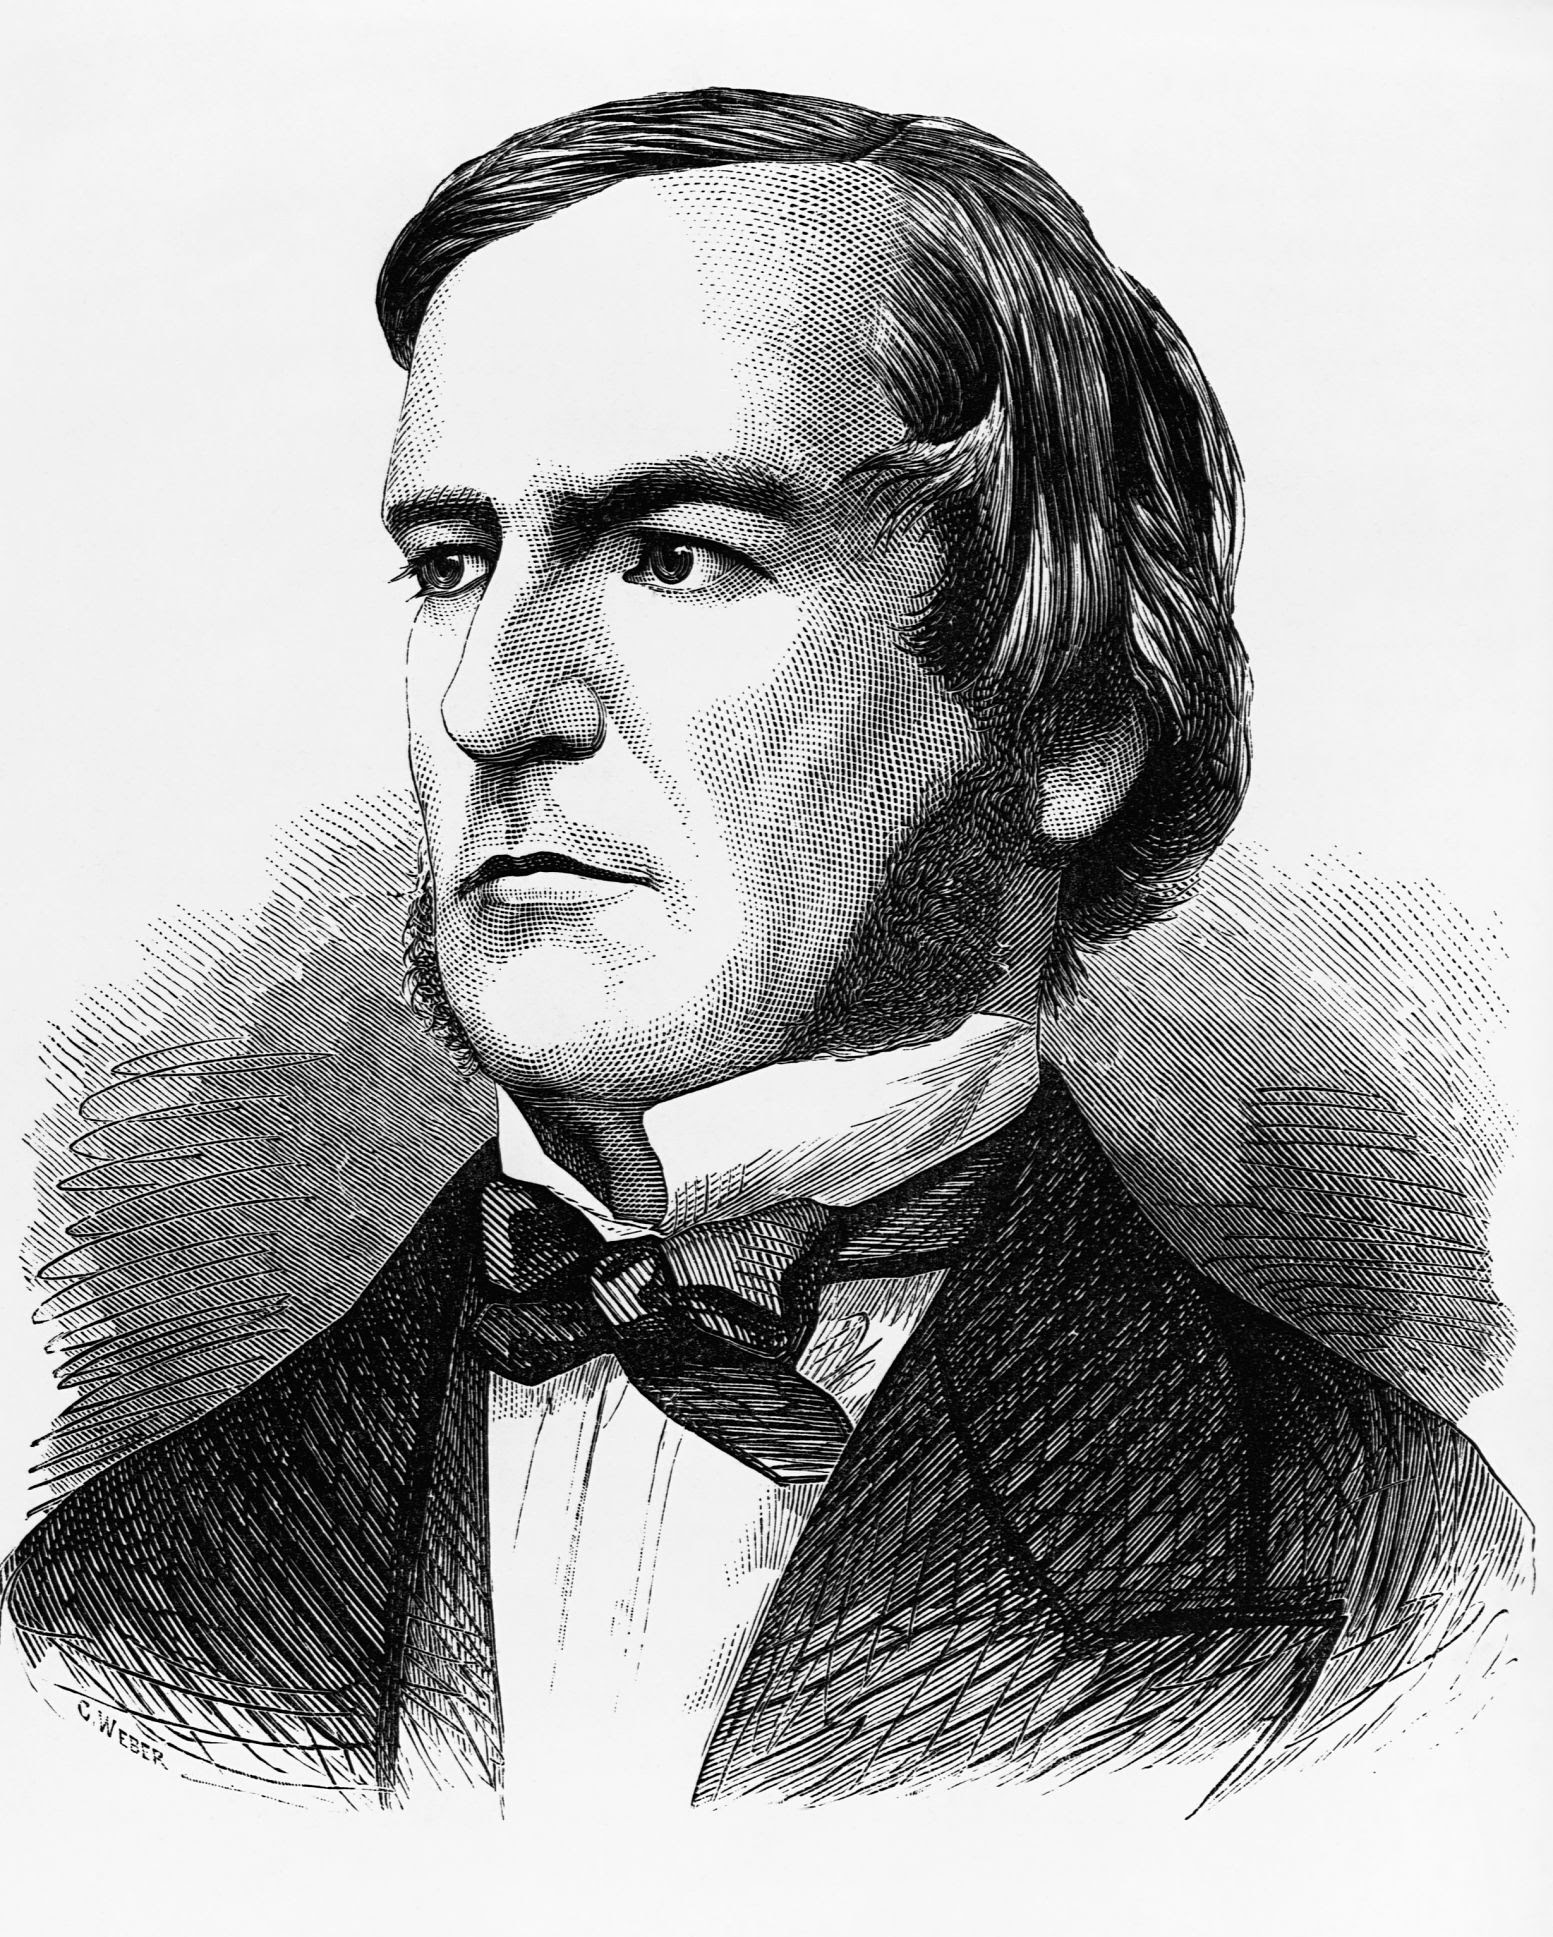
\includegraphics[width=0.36\textwidth]{Images/IMG_0373.jpeg}
}{%
George Boole fue un matemático británico nacido el 2 de noviembre de 1815 en Lincoln, Inglaterra, y fallecido el 8 de diciembre de 1864 en Ballintemple, Irlanda. Es conocido por sus contribuciones pioneras en el campo de la lógica y el álgebra. En 1847, publicó su obra “The Mathematical Analysis of Logic”, donde presentó un sistema algebraico que permitía representar el razonamiento lógico mediante símbolos y ecuaciones, un precursor del Álgebra Booleana, fundamental en la informática y la electrónica. Sus leyes lógicas, conocidas como las “Leyes de Boole”, siguen siendo fundamentales en la teoría de circuitos digitales y la programación. George Boole dejó un legado duradero en las matemáticas y la informática, y su trabajo continúa siendo relevante en la era digital.
}

El Álgebra Booleana, nombrada en honor a George Boole, es un campo fundamental en las Matemáticas Discretas que encuentra sus raíces en la lógica y la teoría de conjuntos. Esta rama de las matemáticas se ha convertido en un pilar esencial en la informática y la ingeniería eléctrica, ya que proporciona un marco formal para el análisis y la manipulación de sistemas que pueden tener solo dos estados: verdadero o falso, 1 o 0 respectivamente. Además, una característica distintiva, es su capacidad para representar problemas complejos mediante ecuaciones booleanas y simplificar estas ecuaciones utilizando reglas algebraicas específicas. Esto es esencial para diseñar circuitos digitales, construir algoritmos eficientes y resolver problemas lógicos de manera sistemática.\\


El Álgebra Booleana se basa en un conjunto de operaciones fundamentales, las cuales son AND, OR y NOT, que permiten combinar y transformar variables booleanas. A partir de estas operaciones básicas, se pueden derivar muchas otras, como XOR (o exclusivo), NAND (NO Y), NOR (NO O), entre otras.

\newpage

\section{Funciones booleanas: Formas normales disyuntiva y conjuntiva}

Como tema preliminar, debemos saber que un interruptor eléctrico puede encenderse (permitiendo el flujo de corriente) o apagarse (evitando el flujo de corriente). Es decir

\begin{center}
    \begin{tabular}{ccccl}
        \begin{circuitikz}
            \draw (1,0) to[short,-*] (2,0);
            \draw[very thick] (2,0) -- +(40:0.8);
            \draw (2.75,0) to[short,*-] (4,0);
        \end{circuitikz} & & 0 & & desactivado \\
        \begin{circuitikz}
            \draw (1,0) to[short,-*] (2,0);
            \draw[very thick] (2,0) -- (2.75,0);
            \draw (2.75,0) to[short,*-] (4,0);
        \end{circuitikz} & & 1 & & activado
    \end{tabular}
\end{center}
Además, tambien tenemos la fuente de energía y la carga respectivamente:
\begin{center}
    \begin{circuitikz}[american,cute inductors][americanvoltages]
        \draw (0,0) to[battery1] (1,0);
        \draw (3,0) to[R] (5,0);
    \end{circuitikz}
\end{center}
Con estos elementos, podemos crear el siguiente circuito en serie:
\begin{center}
    \begin{circuitikz}[american,cute inductors][americanvoltages]
        \draw (0,0) -- (6,0);
        \draw (0,2) to[battery1, v=~] (0,0);
        
        \draw (4.75,2) to[short,*-] (6,2) to[R] (6,0);
        \draw (0,2) to[short,-*, i=~] (2,2);
        \draw[very thick] (2,2) -- +(40:0.8);
        \draw (2.75,2) to[short,*-*] (4,2);
        \draw[very thick] (4,2) -- +(40:0.8);
    \end{circuitikz}
    \captionof{figure}{Ejemplo de circuito en serie}
\end{center}
Del anterior circuito, podemos definir lo siguiente:
\begin{center}
    \begin{tabular}{cc}
        \begin{circuitikz}[american,cute inductors][americanvoltages]
            \draw (0,0) -- (6,0);
            \draw (0,2) to[battery1, v=~] (0,0);
            
            \draw (4.75,2) to[short,*-] (6,2) to[R] (6,0);
            \draw (0,2) to[short,-*, i=~] (2,2);
            \draw[very thick] (2,2) -- +(40:0.8);
            \draw (2.75,2) to[short,*-*] (4,2);
            \draw[very thick] (4,2) -- +(40:0.8);
        \end{circuitikz} & \begin{circuitikz}[american,cute inductors][americanvoltages]
            \draw (0,0) -- (6,0);
            \draw (0,2) to[battery1, v=~] (0,0);
            
            \draw (4.75,2) to[short,*-] (6,2) to[R] (6,0);
            \draw (0,2) to[short,-*, i=~] (2,2);
            \draw[very thick] (2,2) -- +(40:0.8);
            \draw (2.75,2) to[short,*-*] (4,2);
            \draw[very thick] (4,2) -- (4.75,2);
        \end{circuitikz} \\
        $0 \cdot 0 = 0$ & $0 \cdot 1 = 0$ \\
        \begin{circuitikz}[american,cute inductors][americanvoltages]
            \draw (0,0) -- (6,0);
            \draw (0,2) to[battery1, v=~] (0,0);
            
            \draw (4.75,2) to[short,*-] (6,2) to[R] (6,0);
            \draw (0,2) to[short,-*, i=~] (2,2);
            \draw[very thick] (2,2) -- (2.75,2);
            \draw (2.75,2) to[short,*-*] (4,2);
            \draw[very thick] (4,2) -- +(40:0.8);
        \end{circuitikz} & \begin{circuitikz}[american,cute inductors][americanvoltages]
            \draw (0,0) -- (6,0);
            \draw (0,2) to[battery1, v=~] (0,0);
            
            \draw (4.75,2) to[short,*-] (6,2) to[R] (6,0);
            \draw (0,2) to[short,-*, i=~] (2,2);
            \draw[very thick] (2,2) -- (2.75,2);
            \draw (2.75,2) to[short,*-*] (4,2);
            \draw[very thick] (4,2) -- (4.75,2);
        \end{circuitikz} \\
        $1 \cdot 0 = 0$ & $1 \cdot 1 = 1$
    \end{tabular}
\end{center}
Ahora, consideremos un circuito en paralelo:
\begin{center}
    \begin{circuitikz}[american,cute inductors][americanvoltages]
        \draw (0,0) -- (6,0);
        \draw (0,2) to[battery1, v=~] (0,0);
        
        \draw (5,3) to (5,2) to (6,2) to[R] (6,0);
        \draw (0,2) to[short, i=~] (1,2);
        
        \draw (1,2) to (1,3) to[short, i=~, -*] (3,3);
        \draw[very thick] (3,3) -- +(40:0.8);
        \draw (3.75,3) to[short,*-*] (5,3);

        \draw (1,2) to (1,1) to[short, i=~, -*] (3,1);
        \draw[very thick] (3,1) -- +(40:0.8);
        \draw (3.75,1) to[short,*-*] (5,1) to (5,2);
    \end{circuitikz}
    \captionof{figure}{Ejemplo de circuito en paralelo}
\end{center}
Del anterior circuito, podemos definir lo siguiente:
\begin{center}
    \begin{tabular}{cc}
        \begin{circuitikz}[american,cute inductors][americanvoltages]
            \draw (0,0) -- (6,0);
            \draw (0,2) to[battery1, v=~] (0,0);
            
            \draw (5,3) to (5,2) to (6,2) to[R] (6,0);
            \draw (0,2) to[short, i=~] (1,2);
            
            \draw (1,2) to (1,3) to[short, i=~, -*] (3,3);
            \draw[very thick] (3,3) -- +(40:0.8);
            \draw (3.75,3) to[short,*-*] (5,3);
            
            \draw (1,2) to (1,1) to[short, i=~, -*] (3,1);
            \draw[very thick] (3,1) -- +(40:0.8);
            \draw (3.75,1) to[short,*-*] (5,1) to (5,2);
        \end{circuitikz} & \begin{circuitikz}[american,cute inductors][americanvoltages]
            \draw (0,0) -- (6,0);
            \draw (0,2) to[battery1, v=~] (0,0);
            
            \draw (5,3) to (5,2) to (6,2) to[R] (6,0);
            \draw (0,2) to[short, i=~] (1,2);
            
            \draw (1,2) to (1,3) to[short, i=~, -*] (3,3);
            \draw[very thick] (3,3) -- +(40:0.8);
            \draw (3.75,3) to[short,*-*] (5,3);
            
            \draw (1,2) to (1,1) to[short, i=~, -*] (3,1);
            \draw[very thick] (3,1) -- (3.75,1);
            \draw (3.75,1) to[short,*-*] (5,1) to (5,2);
        \end{circuitikz} \\
        $0 + 0 = 0$ & $0 + 1 = 1$ \\
        \begin{circuitikz}[american,cute inductors][americanvoltages]
            \draw (0,0) -- (6,0);
            \draw (0,2) to[battery1, v=~] (0,0);
            
            \draw (5,3) to (5,2) to (6,2) to[R] (6,0);
            \draw (0,2) to[short, i=~] (1,2);
            
            \draw (1,2) to (1,3) to[short, i=~, -*] (3,3);
            \draw[very thick] (3,3) -- (3.75,3);
            \draw (3.75,3) to[short,*-*] (5,3);
            
            \draw (1,2) to (1,1) to[short, i=~, -*] (3,1);
            \draw[very thick] (3,1) -- +(40:0.8);
            \draw (3.75,1) to[short,*-*] (5,1) to (5,2);
        \end{circuitikz} & \begin{circuitikz}[american,cute inductors][americanvoltages]
            \draw (0,0) -- (6,0);
            \draw (0,2) to[battery1, v=~] (0,0);
            
            \draw (5,3) to (5,2) to (6,2) to[R] (6,0);
            \draw (0,2) to[short, i=~] (1,2);
            
            \draw (1,2) to (1,3) to[short, i=~, -*] (3,3);
            \draw[very thick] (3,3) -- (3.75,3);
            \draw (3.75,3) to[short,*-*] (5,3);
            
            \draw (1,2) to (1,1) to[short, i=~, -*] (3,1);
            \draw[very thick] (3,1) -- (3.75,1);
            \draw (3.75,1) to[short,*-*] (5,1) to (5,2);
        \end{circuitikz} \\
        $1 + 0 = 1$ & $1 + 1 = 1$
    \end{tabular}
\end{center}
Sea $B = \{ 0, \, 1 \}$, definimos la suma, producto y complemento para los elementos de $B$ como
\begin{tasks}(2)
    \task $0 + 0 = 0$; $0 + 1 = 1 + 0 = 1 + 1 = 1$
    \task $0 \cdot 0 = 1 \cdot 0 = 0 \cdot 1 = 0$; $1 \cdot 1 = 1$
    \task $\overline{0} = 1$; $\overline{1} = 0$
\end{tasks}

Una variable $x$ es una variable booleana si $x$ solo toma valores de $B$. En consecuencia, tenemos que si $x$, $y \in B$
\begin{tasks}[style=enumerate](2)
    \task $x + x = x$
    \task $x^2 = x \cdot x = x$
    \task $x + y = 0$ si y sólo si $x = 0 = y$
    \task $x \cdot y = 1$ si y sólo si $x = 1 = y$
\end{tasks}

Si $n \in \ZZ[+]$, entonces $B^n = \left\{ (b_1, \, b_2, \, \dots, \, b_n) \mid b_i \in \{0, \, 1\}, \; 1 \leq i \leq n \right\}$. Una función $f: B^n \longrightarrow B$ es una función de conmutación o booleana, de $n$ variables. Las $n$ variables se enfatizan si escribimos $f(x_1, \, x_2, \, \dots, \, x_n)$, donde cada $x_i$, para $1 \leq i \leq n$ es una variable booleana.

\begin{myexample}
    Sea $f:B^3 \longrightarrow B$, donde $f(x, \, y, \, z) = xy + z$. Esta función booleana queda determinada evaluando $f$ para cada una de las ocho posibles asignaciones a las variables $x$, $y$, $z$. Es decir:
    \begin{center}
        \begin{NiceTabular}[hvlines-except-borders,rules={color=white,width=1pt}]{ccccc}
        \CodeBefore
        \rowcolor{jblueleft!80}{1}
        \rowcolors{2}{DodgerBlue3!40}{jblueinner}
        \Body
        \RowStyle[color=white]{}
            $x$ & $y$ & $z$ & $xy$ & $f(x, \, y, \, z) = xy + z$ \\
            0 & 0 & 0 & 0 & 0 \\
            0 & 0 & 1 & 0 & 1 \\
            0 & 1 & 0 & 0 & 0 \\
            0 & 1 & 1 & 0 & 1 \\
            1 & 0 & 0 & 0 & 0 \\
            1 & 0 & 1 & 0 & 1 \\
            1 & 1 & 0 & 1 & 1 \\
            1 & 1 & 1 & 1 & 1
        \end{NiceTabular}
        \captionof{table}{~}
    \end{center}
    Nótese que también podemos escribir a $f$ como $f(x_1, \, x_2, \, x_3)$ siendo $x_1$, $x_2$, $x_3$ variables booleanas.
\end{myexample}

\newpage

\begin{definicion}{}{}
    Para $n \in \ZZ[+]$, $n \geq 2$. Sean $f$, $g: B^n \longrightarrow B$ dos funciones booleanas. Decimos que $f$ y $g$ son iguales y escribiremos $f=g$ si las columnas para $f$ y $g$ son iguales en sus respectivas tablas de función.
\end{definicion}

\begin{definicion}{}{}
    Si $f:B^n \longrightarrow B$, entonces el complemento de $f$, denotado por $\overline{f}$, es la función booleana definida sobre $B^n$ como
    $$\overline{f}(x_1, \, x_2, \, \dots, \, x_n) = \overline{f(x_1, \, x_2, \, \dots, \, x_n)}.$$
    Si $g:B^n \longrightarrow B$, definimos $f + g$, $f \cdot g :B^n \longrightarrow B$ la suma y producto de $f$, $g$, respectivamente como
    $$(f+g)(x_1, \, x_2, \, \dots, \, x_n) = f(x_1, \, x_2, \, \dots, \, x_n) + g(x_1, \, x_2, \, \dots, \, x_n)$$
    y
    $$(f \cdot g)(x_1, \, x_2, \, \dots, \, x_n) = f(x_1, \, x_2, \, \dots, \, x_n) \cdot g(x_1, \, x_2, \, \dots, \, x_n).$$
\end{definicion}

\begin{BOX}
    Las funciones identidad y nula se expresan respectivamente como
    \begin{align*}
        \mathbb{1} : B^n \longrightarrow B \quad \mathbb{0} : B^n \longrightarrow B
    \end{align*}
    donde $\mathbb{1} (x_1, \, x_2, \, \dots, \, x_n) = 1 \in \RR$ y $\mathbb{0} (x_1, \, x_2, \, \dots, \, x_n) = 0 \in \RR$.
\end{BOX}

En la siguiente tabla, se resumen diez leyes, que son consecuencias importantes de las definiciones anteriores:

\begin{center}
    \begin{NiceTabular}[hvlines-except-borders,rules={color=white,width=1pt}]{lll}
        \CodeBefore
        %\rowcolor{jblueleft!80}{1}
        \rowcolors{1}{DodgerBlue3!40}{jblueinner}
        \Body
        %\RowStyle[color=white]{}
        Ley del doble complemento & $\begin{array}{l} \overline{\overline{x}} \end{array}$ & $\begin{array}{l} \overline{\overline{f}} = f \end{array}$ \\
        Leyes de De Morgan & $\begin{array}{l}
            \overline{x+y} = \overline{x} \, \overline{y} \\
            \overline{xy} = \overline{x} + \overline{y}
        \end{array}$ & $\begin{array}{l}
            \overline{f+g} = \overline{f}\overline{g} \\
            \overline{fg} = \overline{f} + \overline{g}
        \end{array}$ \\
        Leyes conmutativas & $\begin{array}{l}
            x+y = y+x \\
            xy = yx
        \end{array}$ & $\begin{array}{l}
            f+g = g+f \\
            fg = gf
        \end{array}$ \\
        Leyes asociativas & $\begin{array}{l}
            x+(y+z) = (x+y)+z \\
            x(yz) = (xy)z
        \end{array}$ & $\begin{array}{l}
            f+(g+h) = (f+g)+h \\
            f(gh) = (fg)h
        \end{array}$ \\
        Leyes distributivas & $\begin{array}{l}
            x+yz = (x+y)(x+z) \\
            x(y+z) = xy + xz
        \end{array}$ & $\begin{array}{l}
            f+gh = (f+g)(f+h) \\
            f(g+h) = fg + fh
        \end{array}$ \\
        Leyes de idempotencia & $\begin{array}{l}
            x + x = x \\
            xx = x
        \end{array}$ & $\begin{array}{l}
            f + f = f \\
            ff = f
        \end{array}$ \\
        Leyes de identidad & $\begin{array}{l}
            x + 0 = x \\
            x \cdot 1 = x
        \end{array}$ & $\begin{array}{l}
            f + \mathbb{0} = f \\
            f \cdot \mathbb{1} = f
        \end{array}$ \\
        Leyes de los inversos & $\begin{array}{l}
            x + \overline{x} = 1 \\
            x \cdot \overline{x} = 0
        \end{array}$ & $\begin{array}{l}
            f + \overline{f} = \mathbb{1} \\
            f \overline{f} = \mathbb{0}
        \end{array}$ \\
        Leyes de dominación & $\begin{array}{l}
            x + 1 = 1 \\
            x \cdot 0 = 0
        \end{array}$ & $\begin{array}{l}
            f + \mathbb{1} = \mathbb{1} \\
            f \cdot \mathbb{0} = \mathbb{0}
        \end{array}$ \\
        Leyes de absorción & $\begin{array}{l}
            x+xy = x \\
            x(x + y) = x
        \end{array}$ & $\begin{array}{l}
            f+fg = f \\
            f(f +g) = f
        \end{array}$
    \end{NiceTabular}
    \captionof{table}{Leyes en el álgebra booleana}\label{table3}
\end{center}
Nótese que  como en las leyes de la lógica de la tabla \ref{table1} (en el capítulo \ref{chap:1}) y las leyes de la teoría de conjuntos de la tabla \ref{table2} (en el capítulo \ref{chap:3}), las propiedades que aparecen en la tabla \ref{table3} son satisfechas por las funciones arbitrarias $f$, $g$, $h: B^n \longrightarrow B$ y por las variables booleanas arbitrarias $x$, $y$, $z$.

\newpage

\begin{myexample}
    Demuestre la Ley distributiva de $+$ sobre $\cdot$, es decir
    $$f(g + h) = fg + fh.$$

    \tcblower
    \textbf{\color{jblueleft}Solución:} Tenemos
    \begin{center}
        \begin{NiceTabular}[hvlines-except-borders,rules={color=white,width=1pt}]{cccccccc}
        \CodeBefore
        \rowcolor{jblueleft!80}{1}
        \rowcolors{2}{DodgerBlue3!40}{jblueinner}
        \Body
        \RowStyle[color=white]{}
            $f$ & $g$ & $h$ & $gh$ & $f+g$ & $f+h$ & $f+gh$ & $(f+g)(f+h)$ \\
            0 & 0 & 0 & 0 & 0 & 0 & 0 & 0 \\
            0 & 0 & 1 & 0 & 0 & 1 & 0 & 0 \\
            0 & 1 & 0 & 0 & 1 & 0 & 0 & 0 \\
            0 & 1 & 1 & 1 & 1 & 1 & 1 & 1 \\
            1 & 0 & 0 & 0 & 1 & 1 & 1 & 1 \\
            1 & 0 & 1 & 0 & 1 & 1 & 1 & 1 \\
            1 & 1 & 1 & 1 & 1 & 1 & 1 & 1
        \end{NiceTabular}
        \captionof{table}{~}
    \end{center}
    Por tanto,
    $$f(g + h) = fg + fh.$$
\end{myexample}

\begin{myexample}
    \begin{enumerate}[label=\alph*)]
        \item Para establecer la primera ley de absorción para las variables booleanas, en vez de basarnos en la construcción de una tabla, argumentamos de la forma siguiente:
        \begin{align*}
            x + xy & = x1 + xy && \text{ley de identidad} \\
            & = x(1+y) && \text{ley distributiva} \\
            & = x1 && \text{ley de dominio} \\
            & = x && \text{ley de identidad}
        \end{align*}
        Este resultado indica que algunas de las leyes pueden deducirse de otras.
        \item Para las variables booleanas $w$, $x$, $y$, $z$, tenemos que
        \begin{align*}
            wx + xy + wz + xz & = (w + x)y + (w + x)z && \text{ley conmutativa} \\
            & = (w + x) (y + z) && \text{ley distributiva}
        \end{align*}
        \item Simplifiquemos la expresión $wx + \overline{\overline{x}z} + \left(y+\overline{z}\right)$, donde $w$, $x$, $y$, $z$ son variables booleanas
        \begin{align*}
            wx + \overline{\overline{x}z} + \left(y+\overline{z}\right) & = wx + \overline{\overline{x}} + \overline{z} + y + \overline{z} && \text{ley de De Morgan} \\
            & = wx + x + \overline{z} + y + \overline{z} && \text{ley del doble complemento} \\
            & = x + \overline{z} + y + \overline{z} && \text{ley de dominación} \\
            & = x + \overline{z} + y && \text{ley de idempotencia}
        \end{align*}
        Por tanto,
        $$wx + \overline{\overline{x}z} + \left(y+\overline{z}\right) = x + \overline{z} + y.$$
    \end{enumerate}
\end{myexample}

\newpage

\begin{myexample}
    Dadas tres variables $x$, $y$, $z$, hallar las expresiones para las funciones $f$, $g$, $h:B^n \longrightarrow B$ de acuerdo a la siguiente tabla:
    \begin{center}
        \begin{NiceTabular}[hvlines-except-borders,rules={color=white,width=1pt}]{cccccc}
        \CodeBefore
        \rowcolor{jblueleft!80}{1}
        \rowcolors{2}{DodgerBlue3!40}{jblueinner}
        \Body
        \RowStyle[color=white]{}
            $x$ & $y$ & $z$ & $f$ & $g$ & $h$ \\
            0 & 0 & 0 & 0 & 0 & 0 \\
            0 & 0 & 1 & 1 & 0 & 1 \\
            0 & 1 & 0 & 0 & 0 & 0 \\
            0 & 1 & 1 & 0 & 0 & 0 \\
            1 & 0 & 0 & 0 & 1 & 1 \\
            1 & 0 & 1 & 0 & 0 & 0 \\
            1 & 1 & 0 & 0 & 0 & 0 \\
            1 & 1 & 1 & 0 & 0 & 0
        \end{NiceTabular}
        \captionof{table}{~}
    \end{center}

    \tcblower
    \textbf{\color{jblueleft}Solución:} Para la columna que está debajo de $f$, queremos un resultado que tenga el valor 1 cuando $x = y = 0$ y $z = 1$. La función $f(x, \, y, \, z) = \overline{x} \bar{y} z$ es una de las funciones que deseamos. De la misma manera, $g(x, \, y, \, z) = x \overline{y} \bar{z}$ da el valor 1 para $x = 1$, $y = z = 0$ y 0 en los demás casos. Como $f$ y $g$ tienen el valor 1 solamente en un caso y estos casos son distintos entre sí, su suma $f + g$ toma el valor 1 exactamente en estos dos casos. Así, $h(x, \, y, \, z) = f(x, \, y, \, z) + g(x, \, y, \, z) = \overline{x} \bar{y} z + x \overline{y} \bar{z}$ tiene la columna de valores dados bajo $h$. Evaluando las funciones que propusimos en cada variable $x$, $y$, $z$ dadas en la tabla anterior, obtenemos
    \begin{align*}
        f(x, \, y, \, z) & = \overline{x} \bar{y} z & g(x, \, y, \, z) & = x \overline{y} \bar{z} & h(x, \, y, \, z) & = f(x, \, y, \, z) + g(x, \, y, \, z) \\
        f(0, \, 0, \, 0) & = \overline{0} \cdot \overline{0} \cdot 0 = 0 & g(0, \, 0, \, 0) & = 0 \cdot \overline{0} \cdot \overline{0} = 0 & h(0, \, 0, \, 0) & = 0 + 0 = 0 \\
        f(0, \, 0, \, 1) & = \overline{0} \cdot \overline{0} \cdot 1 = 1 & g(0, \, 0, \, 1) & = 0 \cdot \overline{0} \cdot \overline{1} = 0 & h(0, \, 0, \, 1) & = 1 + 0 = 1 \\
        f(0, \, 1, \, 0) & = \overline{0} \cdot \overline{1} \cdot 0 = 0 & g(0, \, 1, \, 0) & = 0 \cdot \overline{1} \cdot \overline{0} = 0 & h(0, \, 1, \, 0) & = 0 + 0 = 0 \\
        f(0, \, 1, \, 1) & = \overline{0} \cdot \overline{1} \cdot 1 = 0 & g(0, \, 1, \, 1) & = 0 \cdot \overline{1} \cdot \overline{1} = 0 & h(0, \, 1, \, 1) & = 0 + 0 = 0 \\
        f(1, \, 0, \, 0) & = \overline{1} \cdot \overline{0} \cdot 0 = 0 & g(1, \, 0, \, 0) & = 1 \cdot \overline{0} \cdot \overline{0} = 1 & h(1, \, 0, \, 0) & = 0 + 1 = 1 \\
        f(1, \, 0, \, 1) & = \overline{1} \cdot \overline{0} \cdot 1 = 0 & g(1, \, 0, \, 1) & = 1 \cdot \overline{0} \cdot \overline{1} = 0 & h(1, \, 0, \, 1) & = 0 + 0 = 0 \\
        f(1, \, 1, \, 0) & = \overline{1} \cdot \overline{1} \cdot 0 = 0 & g(1, \, 1, \, 0) & = 0 \cdot \overline{0} \cdot \overline{0} = 0 & h(1, \, 1, \, 0) & = 0 + 0 = 0 \\
        f(1, \, 1, \, 1) & = \overline{1} \cdot \overline{1} \cdot 1 = 0 & g(1, \, 1, \, 1) & = 1 \cdot \overline{1} \cdot \overline{1} = 0 & h(1, \, 1, \, 1) & = 0 + 0 = 0
    \end{align*}
    que es justo lo que queríamos que cumpliera.
\end{myexample}

\begin{definicion}{}{}
    Para cualquier $n \in \ZZ[+]$, si $f$ es una función booleana sobre las $n$ variables $x_1$, $x_2$, $\dots$, $x_n$
    \begin{enumerate}[label=\alph*)]
        \item cada término $x_i$ o su complemento $\overline{x_i}$, para $1 \leq i \leq n$ es una \textbf{literal}
        \item un término de la forma $y_1 y_2 \cdots y_n$ en donde cada $y_i = x_i$ o $y_i = \overline{x_i}$, para $1 \leq i \leq n$ se le llama conjunción fundamental o minitérmino (termin)
        \item una representación de $f$ como una suma de conjunciones fundamentales es una forma normal disyuntiva (f.n.d) de $f$.
    \end{enumerate}
\end{definicion}

\newpage

\begin{myexample}
    Encuentre la f.n.d de $f:B^3 \longrightarrow B$ donde $f(x, \, y, \ z) = xy + \overline{x} z$.
    
    \tcblower
    \textbf{\color{jblueleft}Solución:}
    De la siguiente tabla
    \begin{center}
        \begin{NiceTabular}[hvlines-except-borders,rules={color=white,width=1pt}]{cccccc}
        \CodeBefore
        \rowcolor{jblueleft!80}{1}
        \rowcolors{2}{DodgerBlue3!40}{jblueinner}
        \Body
        \RowStyle[color=white]{}
            $x$ & $y$ & $z$ & $xy$ & $\overline{x}z$ & $f$ \\
            0 & 0 & 0 & 0 & 0 & 0 \\
            0 & 0 & 1 & 0 & 1 & 1 \\
            0 & 1 & 0 & 0 & 0 & 0 \\
            0 & 1 & 1 & 0 & 1 & 1 \\
            1 & 0 & 0 & 0 & 0 & 0 \\
            1 & 0 & 1 & 0 & 0 & 0 \\
            1 & 1 & 0 & 1 & 0 & 0 \\
            1 & 1 & 1 & 1 & 0 & 1
        \end{NiceTabular}
        \captionof{table}{~}
    \end{center}
    vemos que la columna de $f$ tiene cuatro unos, los cuales nos indican las cuatro conjunciones fundamentales necesarias en la f.n.d de $f$, de modo que $f(x, \, y, \ z) = \overline{x} \bar{y} z + \overline{x} y z + x y \overline{z} +  xyz$. Imaginemos que no tuvieramos la tabla anterior, para obtener la f.n.d de $f$ sin tabla se procede como:
    \begin{align*}
        f(x, \, y, \ z) & = xy + \overline{x}z \\
        & = xy \cdot 1 + \overline{x} \cdot 1 \cdot z \\
        & = xy (z+\overline{z}) + \overline{x}(y+\overline{y})z \\
        & = xyz + xy\overline{z} + (\overline{x}y+\overline{x}\bar{y})z \\
        & = xyz +  xy\overline{z} + \overline{x}yz + \overline{x}\bar{y}z
    \end{align*}
    que es lo mismo que obtuvimos anteriormente.
\end{myexample}

\begin{BOX}
    Las funciones se pueden expresar de forma simplificada, al usar la etiqueta binaria, se escribiría como suma de termins. Tomando la función del ejemplo anterior:
    $$f = \sum m(1, \, 3, \, 6, \, 7) \quad \text{donde } m \text{ indica los minitérminos}.$$
\end{BOX}

\begin{myexample}
    Encuentre la f.n.d de $g:B^4 \longrightarrow B$ donde $g(w, \, x, \, y, \ z) = wx\overline{y} + wy\overline{z} + xy$.

    \tcblower
    \textbf{\color{jblueleft}Solución:} Obtengamos la f.n.d de $g$ sin tabla como en el anterior ejemplo. Entonces
    \begin{align*}
        g(w, \, x, \, y, \ z) & = wx\overline{y} (z+\overline{z}) + w(x+\overline{x})y\overline{z} + xy(z+\overline{z}) \\
        & = wx\overline{y} z + wx\overline{y}\overline{z} + wxy\overline{z} + w\overline{x}y\overline{z} + xyz + xy\overline{z} \\
        & = wx\overline{y} z + wx\overline{y}\overline{z} + wxy\overline{z} + w\overline{x}y\overline{z} + (w+\overline{w})xyz + (w+\overline{w})xy\overline{z} \\
        & = wx\overline{y} z + wx\overline{y}\overline{z} + wxy\overline{z} + w\overline{x}y\overline{z} + wxyz + \overline{w}xyz + wxy\overline{z} + \overline{w}xy\overline{z}
    \end{align*}
    Por la propiedad idempotente
    $$g(w, \, x, \, y, \ z) = wx\overline{y}z + wx\overline{y}\bar{z} + wxy\overline{z} + w\overline{x}y\overline{z} + wxyz + \overline{w}xyz + \overline{w}xy\overline{z}.$$
\end{myexample}

\newpage

\begin{BOX}
    Expresemos a $g$ del ejemplo anterior en forma simplicada. Tenemos entonces
    $$\begin{array}{llr}
        wx\overline{y}z & 1101 & 13 \\
        wx\overline{y}\bar{z} & 1100 & 12 \\
        wxy\overline{z} & 1110 & 14 \\
        w\overline{x}y\overline{z} & 1010 & 10 \\
        wxyz & 1111 & 15 \\
        \overline{w}xyz & 0111 & 7 \\
        \overline{w}xy\overline{z} & 0110 & 6
    \end{array}$$
    donde la tercer columna es la etiqueta binaria. Así pues,
    $$g = \sum m(6, \, 7, \, 10, \, 12, \, 13, \, 14, \, 15).$$
\end{BOX}

\begin{definicion}{}{}
    Para cualquier $n \in \ZZ[+]$, si $f$ es una función booleana sobre las $n$ variables $x_1$, $x_2$, $\dots$, $x_n$
    \begin{enumerate}[label=\alph*)]
        \item cada término $x_i$ o su complemento $\overline{x_i}$, para $1 \leq i \leq n$ es una \textbf{literal}
        \item un término de la forma $c_1 + c_2 + \cdots + c_n$ en donde cada $c_i = x_i$ o $c_i = \overline{x_i}$, para $1 \leq i \leq n$ se le llama disyunción fundamental o maxitérmino (termix)
        \item una representación de $f$ como producto de disyunciones fundamentales es una forma normal conjuntiva (f.n.c) de $f$.
    \end{enumerate}
\end{definicion}

\begin{myexample}
    Hallar la f.n.c para la siguiente función:
    \begin{center}
        \begin{NiceTabular}[hvlines-except-borders,rules={color=white,width=1pt}]{cccc}
        \CodeBefore
        \rowcolor{jblueleft!80}{1}
        \rowcolors{2}{DodgerBlue3!40}{jblueinner}
        \Body
        \RowStyle[color=white]{}
            $x$ & $y$ & $z$ & $f$ \\
            0 & 0 & 0 & 0 \\
            0 & 0 & 1 & 1 \\
            0 & 1 & 0 & 0 \\
            0 & 1 & 1 & 1 \\
            1 & 0 & 0 & 1 \\
            1 & 0 & 1 & 1 \\
            1 & 1 & 0 & 0 \\
            1 & 1 & 1 & 1
        \end{NiceTabular}
    \end{center}

    \tcblower
    \textbf{\color{jblueleft}Solución:} Proponemos a $f: B^3 \longrightarrow B$ donde $f(x, \, y, \, z) = (x+y+z)(x+\overline{y}+z)(\overline{x}+\overline{y}+z)$, pues
    \begin{align*}
        f(0, \, 0, \, 1) & = (0 + 0 + 1)(0 + 1 + 1)(1 + 1 + 1) = 1 \\
        f(0, \, 1, \, 1) & = (0 + 1 + 1)(0 + 0 + 1)(1 + 0 + 1) = 1 \\
        f(1, \, 0, \, 0) & = (1 + 0 + 0)(1 + 1 + 0)(0 + 1 + 0) = 1 \\
        f(1, \, 0, \, 1) & = (1 + 0 + 1)(1 + 1 + 1)(0 + 1 + 1) = 1 \\
        f(1, \, 1, \, 1) & = (1 + 1 + 1)(1 + 0 + 1)(0 + 0 + 1) = 1
    \end{align*}
    y en las demás evaluaciones obtenemos 0. Por tanto, la f.n.c de $f$ se puede expresar como
    $$f = \prod M(0, \, 2, \, 6) \quad \text{donde } M \text{ indica los maxitérminos}.$$
\end{myexample}

\newpage

\begin{myexample}
    Sea $g: B^4 \longrightarrow B$ con $g(w, \, x, \, y, \, z) = (w + x + y)(x + \overline{y} + z)(w + \overline{y})$. Obtengamos la f.n.c de $g$ como sigue:
    \begin{align*}
        g(w, \, x, \, y, \, z) & = (w + x + y)(x + \overline{y} + z)(w + \overline{y}) \\
        & = (w + x + y + z\overline{z})(w\overline{w} + x + \overline{y} + z)(x\overline{x} + w + \overline{y}) \\
        & = (w + x + y + z)(w + x + y + \overline{z})(x + \overline{y} + z + w) \\
        & \hspace{2cm} (x + \overline{y} + z + \overline{w})(x + w + \overline{y})(\overline{x} + w + \overline{y}) \\
        & = (w + x + y + z)(w + x + y + \overline{z})(x + \overline{y} + z + w) \\
        & \hspace{2cm} (x + \overline{y} + z + \overline{w})(x + w + \overline{y} + z\overline{z})(\overline{x} + w + \overline{y} + z\overline{z}) \\
        %& = (w + x + y + z)(w + x + y + \overline{z})(x + \overline{y} + z + w)(x + \overline{y} + z + \overline{w}) \\
        %& \hspace{2cm} (x + w + \overline{y} + z)(\overline{x} + w + \overline{y} + z)(\overline{x} + w + \overline{y} + \overline{z})(x + w + \overline{y} + \overline{z}) \\
        & = (w + x + y + z)(w + x + y + \overline{z})(w + x + \overline{y} + z)(\overline{w} + x + \overline{y} + z) \\
        & \hspace{2cm} (w + \overline{x} + \overline{y} + z)(w + \overline{x} + \overline{y} + \overline{z})(w + x + \overline{y} + \overline{z})
    \end{align*}
    Expresemos en forma simplificada como producto de termax. Tenemos entonces
    $$\begin{array}{llr}
        w+x+y+z & 0000 & \cellcolor{DodgerBlue3!40}{0} \\
        w+x+y+\overline{z} & 0001 & \cellcolor{DodgerBlue3!40}{1} \\
        w+x+\overline{y}+z & 0010 & \cellcolor{DodgerBlue3!40}{2}
    \end{array} \quad \begin{array}{llr}
        \overline{w}+x+\overline{y}+z & 1010 & \cellcolor{DodgerBlue3!40}{10} \\
        w+\overline{x}+\overline{y}+z & 0110 & \cellcolor{DodgerBlue3!40}{6} \\
        w+\overline{x}+\overline{y}+\overline{z} & 0111 & \cellcolor{DodgerBlue3!40}{7}
    \end{array} \quad \begin{array}{llr}
        w+x+\overline{y}+\overline{z} & 0011 & \cellcolor{DodgerBlue3!40}{3}
    \end{array}$$
    donde la tercer columna es la etiqueta binaria respectivamente. Por tanto, la f.n.c de $f$ se puede expresar como 
    $$\displaystyle g = \prod M(0, \, 1, \, 2, \, 3, \, 6, \, 7, \, 10).$$
\end{myexample}

\begin{myexample}
    Sea $h(w, \, x, \, y, \, z) = wx + \overline{w}y + \overline{x}yz$. Hallemos la f.n.d de $h$, entonces
    \begin{align*}
        h(w, \, x, \, y, \, z) & = wx(y + \overline{y}) + \overline{w}(x + \overline{x})y + (w + \overline{w})\overline{x}yz \\
        & = wxy + wx\overline{y} + \overline{w}xy + \overline{w} \overline{x}y + w \overline{x}yz + \overline{w}\overline{x}yz \\
        & = wxy(z + \overline{z}) + wx\overline{y}(z + \overline{z}) + \overline{w}xy(z + \overline{z}) + \overline{w} \overline{x}y(z + \overline{z}) + w \overline{x}yz + \overline{w}\overline{x}yz \\
        %& = wxyz + wxy\overline{z} + wx\overline{y}z + wx\overline{y}\overline{z} + \overline{w}xyz + \overline{w}xy\overline{z} + \overline{w} \overline{x}yz + \overline{w} \overline{x}y\overline{z} + w \overline{x}yz + \overline{w}\overline{x}yz \\
        & = wxyz + wxy\overline{z} + wx\overline{y}z + wx\overline{y}\overline{z} + \overline{w}xyz + \overline{w}xy\overline{z} + \overline{w} \overline{x}yz + \overline{w} \overline{x}y\overline{z} + w \overline{x}yz
    \end{align*}
    Consideremos cada conjunción fundamental en la f.n.d. de $h$, obtenemos lo siguiente:
    $$\begin{array}{llr}
        wxyz & 1111 & \cellcolor{DodgerBlue3!40}{15} \\
        wxy\overline{z} & 1110 & \cellcolor{DodgerBlue3!40}{14} \\
        wx\overline{y}z & 1101 & \cellcolor{DodgerBlue3!40}{13}
    \end{array} \quad \begin{array}{llr}
        wx\overline{y}\overline{z} & 1100 & \cellcolor{DodgerBlue3!40}{12} \\
        \overline{w}xyz & 0111 & \cellcolor{DodgerBlue3!40}{7} \\
        \overline{w}xy\overline{z} & 0110 & \cellcolor{DodgerBlue3!40}{6}
    \end{array} \quad \begin{array}{llr}
        \overline{w} \overline{x}yz & 0011 & \cellcolor{DodgerBlue3!40}{3} \\
        \overline{w} \overline{x}y\overline{z} & 0010 & \cellcolor{DodgerBlue3!40}{2} \\
        w \overline{x}yz & 1011 & \cellcolor{DodgerBlue3!40}{11}
    \end{array}$$
    donde la tercer columna es la etiqueta binaria respectivamente. En consecuencia, también podemos escribir $\displaystyle h = \sum m (2, \, 3, \, 6, \, 7, \, 11, \, 12, \, 13, \, 14, \, 15)$. De esta representación, usando mintérminos, tenemos $\displaystyle h = \prod M (0, \, 1, \, 4, \, 5, \, 8, \, 9, \, 10)$, un producto de maxitérminos. Por último, tomamos la etiqueta en binario de cada maxitérmino y determinamos su disyunción fundamental correspondiente:
    $$\begin{array}{llr}
        w+x+y+z & 0000 & \cellcolor{DodgerBlue3!40}{0} \\
        w+x+y+\overline{z} & 0001 & \cellcolor{DodgerBlue3!40}{1} \\
        w+\overline{x}+y+z & 0010 & \cellcolor{DodgerBlue3!40}{4}
    \end{array} \quad \begin{array}{llr}
        w+\overline{x}+y+\overline{z} & 0101 & \cellcolor{DodgerBlue3!40}{5} \\
        \overline{w}+x+y+z & 1000 & \cellcolor{DodgerBlue3!40}{8} \\
        \overline{w}+x+y+\overline{z} & 1001 & \cellcolor{DodgerBlue3!40}{9}
    \end{array} \quad \begin{array}{llr}
        \overline{w}+x+\overline{y}+z & 1010 & \cellcolor{DodgerBlue3!40}{10}
    \end{array}$$
    Es decir, la f.n.c de $h$ es
    \begin{align*}
        & (w+x+y+z)(w+x+y+\overline{z})(w+\overline{x}+y+z)(w+\overline{x}+y+z) \\
        & \hspace{4cm} (w+\overline{x}+y+\overline{z})(\overline{w}+x+y+z)(\overline{w}+x+y+\overline{z})(\overline{w}+x+\overline{y}+z).
    \end{align*}
\end{myexample}

\chapterimage{blue9.jpeg} % Imagen de encabezado de capítulo
\chapterspaceabove{6.75cm} % Espacio en blanco desde la parte superior de la página hasta el título del capítulo en las páginas del capítulo
\chapterspacebelow{7.25cm} % Cantidad de espacio en blanco vertical desde el margen superior hasta el comienzo del texto en las páginas de los capítulos

%------------------------------------------------

\chapter{RELACIONES Y FUNCIONES}\label{chap:5}


En el apasionante universo de las Matemáticas Discretas, el concepto de relaciones y funciones juega un papel central. Estas ideas fundamentales constituyen la base de muchas ramas de las matemáticas y tienen aplicaciones prácticas en diversas disciplinas, desde la informática hasta la teoría de grafos y la ciencia de datos. En este capítulo, exploraremos minuciosamente el concepto de relaciones y funciones, desentrañando sus propiedades, aplicaciones y conexiones con otros temas dentro de las Matemáticas Discretas.


En esencia, una relación es una conexión entre elementos de dos conjuntos, mientras que una función es una relación especial que asigna de manera única un elemento de un conjunto a otro. Estos conceptos pueden parecer abstractos al principio, pero en realidad, están presentes en la vida cotidiana. Desde las redes sociales que conectan a las personas hasta las operaciones matemáticas que relacionan números, las relaciones y funciones desempeñan un papel esencial en nuestra comprensión del mundo que nos rodea.


A lo largo de este capítulo, exploraremos una variedad de temas importantes, tales como:

\begin{enumerate}
    \item Tipos de relaciones: Aprenderemos acerca de relaciones reflexivas, simétricas y transitivas, así como relaciones de equivalencia y orden parcial.
    \item Funciones: Analizaremos en detalle qué es una función, sus propiedades, dominio, codominio y la importancia de las funciones biyectivas.
    \item Composición de funciones: Descubriremos cómo combinar funciones para crear nuevas funciones y entenderemos la noción de funciones inversas.
    %\item Aplicaciones en la vida real: Exploraremos aplicaciones prácticas de relaciones y funciones en áreas como la informática, la criptografía y la teoría de bases de datos.
\end{enumerate}

Al finalizar este capítulo, habrá desarrollado habilidades sólidas en la identificación y manipulación de relaciones y funciones. También comprenderá cómo estas ideas desempeñan un papel vital en la resolución de problemas complejos y en la modelización de sistemas del mundo real.\\


Este capítulo servirá como base sólida para abordar temas posteriores en Matemáticas Discretas, como la teoría de conjuntos, la teoría de números y la teoría de grafos. Además, proporcionará una base esencial para aquellos que buscan aplicar estas ideas en disciplinas relacionadas con la informática, la ingeniería y las ciencias exactas.

\newpage

\section{Productos cartesianos y relaciones}

\begin{definicion}{}{}
    Sean $A$ y $B$ conjuntos. Si $A \neq \phi$ y $B \neq \phi$, se define el producto cartesiano de $A$ y $B$, denotado por $A \times B$, como el conjunto
    $$A \times B = \{(a, \, b) \mid a \in A \text { y } b \in B\}$$
    y si $A = \phi$ o $B = \phi$, se define $A \times B = \phi$. La expresión $A \times B$ se lee: $A$ cruz $B$ o el producto cartesiano de $A$ y $B$.
\end{definicion}

\begin{BOX}
    Si $A$, $B$ son finitos, se sigue de la regla del producto que $|A \times B| = |A| \cdot |B| = |B \times A|$.
\end{BOX}

\begin{myexample}
    Sean $U = \{ 1, \, 2, \, 3, \, 4, \, 5, \, 6, \, 7 \}$, $A = \{ 2, \, 3, \, 4 \}$, $B = \{ 4, \, 5 \}$. Entonces
    \begin{enumerate}[label=\alph*)]
        \item $A \times B = \{ (2, \, 4), \, (2, \, 5), \, (3, \, 4), \, (3, \, 5), \, (4, \, 4), \, (4, \, 5) \}$.
        \item $B \times A = \{ (4, \, 2), \, (4, \, 3), \, (4, \, 4), \, (5, \, 2), \, (5, \, 3), \, (5, \, 4) \}$.
        \item $B \times B = \{ (4, \, 4), \, (4, \, 5), \, (5, \, 4), \, (5, \, 5) \}$.
    \end{enumerate}
\end{myexample}

\begin{obs}{}{}
    Del ejemplo anterior se sigue que, en general, $A \times B \neq B \times A$.
\end{obs}

\begin{definicion}{}{}
    Sean $A_1, \, A_2, \, \dots, \, A_n$ conjuntos. Si $A_i \neq \phi, \, \forall i=1, \, 2, \, \dots, \, n$, se define el producto cartesiano de $A_1, \, A_2, \, \dots, \, A_n$, denotado por $A_1 \times A_2 \times \dots \times A_n$, como el conjunto
    $$A_1 \times A_2 \times \cdots \times A_n=\left\{\left(a_1, \, a_2, \, \dots, \, a_n\right) \mid a_i \in A_i, \, \forall i=1, \, \dots, \, n\right\}.$$
\end{definicion}

\begin{definicion}{}{}
    Sean $A_1, \, A_2, \, \dots, \, A_n$ conjuntos. Si $A_i=\phi$, para algún $i=1, \,2, \, \dots, \, n$, se define
    $$A_1 \times A_2 \times \cdots \times A_n=\phi.$$
\end{definicion}

\begin{definicion}{}{}
    Si $A$ es un conjunto y $n \in \mathbb{N}$, definimos $A^n$ como
    $$A^n=\underbrace{A \times A \times \cdots \times A}_{n-\text{veces}}.$$
\end{definicion}

\begin{myexample}
    Si $A$ es un conjunto distinto del vacío, entonces: $A^2=A \times A$ y $A^3=A \times A \times A$.
\end{myexample}

\begin{definicion}{}{KANSKKUSJS}
    Para los conjuntos $A$, $B \subseteq U$, cualquier subconjunto $A \times B$ es una \textbf{relación} de $A$ en $B$. Cualquier subconjunto de $A \times A$ es una \textbf{relación binaria} en $A$. Dicha relación la denotaremos por $\mathcal{R}$.
\end{definicion}

\newpage

\begin{myexample}
    Si $U = \RR$, se define a $\RR \times \RR = \RR[2] = \{ (x, \, y) \mid x, \, y \in \RR \}$. A este conjunto se le  reconoce como el plano real de la geometría con coordenadas. Geométricamente se representa como sigue:
    \begin{center}
        \begin{tikzpicture}
            \draw[step=1.0,gray,very thin,dash pattern=on 3pt off 2pt] (0,0) grid (4,4);
            
            \draw[thick,arrows = {-Stealth[scale width=1]}] (-0.5,0) -- (4.4,0);
            \draw[thick,arrows = {-Stealth[scale width=1]}] (0,-0.5) -- (0,4.4);
            \foreach \x in {1,2,3,4} \draw (\x,0.3) -- (\x,0) node[below] {$\x$};
            \foreach \x in {1,2,3,4} \draw (0.3,\x) -- (0,\x) node[left] {$\x$};
        \end{tikzpicture}
        \captionof{figure}{Representación de $\RR[2] = \{ (x, \, y) \mid x, \, y \in \RR \}$}
    \end{center}
\end{myexample}

\begin{myexample}
    Sean $U = \{ 1, \, 2, \, 3, \, 4, \, 5, \, 6, \, 7 \}$, $A = \{ 2, \, 3, \, 4 \}$, $B = \{ 4, \, 5 \}$. Las siguientes son relaciones de $A$ en $B$
    \begin{tasks}(3)
        \task $\phi$
        \task $\{ (2, \, 4) \}$
        \task $\{ (2, \, 4), \, (2, \, 5) \}$
        \task $\{ (2, \, 4), \, (3, \, 4), \, (4, \, 4) \}$
        \task $\{ (2, \, 4), \, (3, \, 4), \, (4, \, 5) \}$
        \task $A \times B$
    \end{tasks}
    Como $|A \times B| = 6$, se sigue de la definición \ref{definicion:KANSKKUSJS} que existen $2^6$ posibles relaciones de $A$ en $B$.
\end{myexample}

\begin{BOX}
    En general, para conjuntos finitos $A$, $B$ con $|A| = m$ y $|B| = n$, existen $2^{mn}$ relaciones de $A$ en $B$, incluyendo la relación vacía y la propia relación $A \times B$.
\end{BOX}

\begin{myexample}
    Con $A = U = \ZZ[+]$, podemos definir una relación binaria en el conjunto $A$ como $\{ (x, \, y) \mid x \leq y \}$. Geométricamente se representa como sigue:
    \begin{center}
        \begin{tikzpicture}
            \draw[step=1.0,gray,very thin,dash pattern=on 3pt off 2pt] (0,0) grid (4,4);
            
            \draw[thick,arrows = {-Stealth[scale width=1]}] (-0.5,0) -- (4.4,0);
            \draw[thick,arrows = {-Stealth[scale width=1]}] (0,-0.5) -- (0,4.4);

            \foreach \x in {1,2,3,4} \filldraw (1,\x) circle (2pt);
            \foreach \x in {2,3,4} \filldraw (2,\x) circle (2pt);
            \foreach \x in {3,4} \filldraw (3,\x) circle (2pt);
            \foreach \x in {4} \filldraw (4,\x) circle (2pt);
            \foreach \x in {1,2,3,4} \draw (\x,0.3) -- (\x,0) node[below] {$\x$};
            \foreach \x in {1,2,3,4} \draw (0.3,\x) -- (0,\x) node[left] {$\x$};
        \end{tikzpicture}
        \captionof{figure}{Representación de $\{ (x, \, y) \mid x \leq y \}$}
    \end{center}
    De la figura precedente, tenemos que $(7, \, 7)$, $(7, \, 11) \in \mathcal{R}$, pero $(8, \, 2) \notin \mathcal{R}$.
\end{myexample}

\newpage

\begin{BOX}
    Cuando un compilador (lenguaje de programación) traduce un programa fuente al lenguaje maquina, este elabora una tabla de símbolos que contiene los siguientes conjuntos:
    \begin{enumerate}
        \item $S$: El conjunto de nombres simbólicos; como variables, constantes y tipos.
        \item $A$: El conjunto de posibles atributos para los elementos de $S$; como entero, real, booleano, carácter, etc.
        \item $L$: El conjunto de posiciones, o direcciones de la memoria en donde se almacena los elementos de $S$.
    \end{enumerate}
\end{BOX}

Para concluir esta sección, consideremos los siguientes incisos: Dados $A$, $B$, $C \subseteq U$
\begin{tasks}(2)
    \task $A \times (B \cup C) = (A \times B) \cap (A \times C)$
    \task $A \times (B \cup C) = (A \times B) \cup (A \times C)$
    \task $(A \cap B) \times C = (A \times C) \cap (B \times C)$
    \task $(A \cup B) \times C = (A \times C) \cup (B \times C)$
\end{tasks}

\section{Funciones: en general e inyectivas}

\begin{definicion}{}{}
    Para los conjuntos no vacíos $A$, $B$, una función, o transformación, $f$ de $A$ hacia $B$, que se denota con $f: A \longrightarrow B$, es una relación de $A$ hacia $B$ en la que cada elemento de $A$ \textbf{aparece exactamente una vez} como la primera componente de un par ordenado en la relación.
\end{definicion}

\begin{myexample}
    \label{jhbhdchsdfbj}
    Si $A = \{1, \, 2, \, 3 \}$ y $B = \{ w, \, x, \, y, \, z \}$, $f = \{ (1, \, w), \, (2, \, x), \, (3, \, x) \}$ es una función, y en consecuencia una relación, de $A$ en $B$. $\mathcal{R}_1 = \{ (1, \, w), \, (2, \, x) \}$ y $\mathcal{R}_2 = \{ (1, \, w), \, (2, \, w), \, (2, \, x), \, (3, \, 2) \}$ son relaciones, pero no funciones, de $A$ en $B$.
\end{myexample}

\begin{definicion}{}{}
    Para la función $f: A \longrightarrow B$, $A$ es el dominio de $f$ y $B$ es el codominio de $f$. El subconjunto de $B$ formado por aquellos elementos que aparecen como segundas componentes de los pares ordenados de $f$ se conoce como la imagen de $f$ y se denota también como $f(A)$ ya que es el conjunto de imágenes (de los elementos de $A$) mediante $f$.
\end{definicion}

\begin{myexample}
    En el ejemplo anterior, el dominio de $f$ es $\{1, \, 2, \, 3\}$, el codominio de $f$ es $\{w, \, x, \, y, \, z\}$ y la imagen de $f$ es $f(A) = \{w, \, x\}$.\\
    Una representación gráfica de estas ideas aparecen en la figura \ref{KSKSKKSKSKSKKDND}. Este diagrama sugiere que $a$ puede verse como una entrada que es transformada por $f$ en la salida correspondiente, $f(a)$.
    \begin{center}
        \begin{tikzpicture}[x=0.75pt,
        y=0.75pt,
        yscale=-1,
        xscale=1,
        scale=0.55
        ]
            %Shape: Polygon Curved [id:ds23961530607472992] 
            \draw  [draw opacity=0][fill=SteelBlue1,fill opacity=1 ] (96.5,87) .. controls (158,2) and (223,84) .. (229.5,119) .. controls (236,154) and (237.5,191) .. (208.5,196) .. controls (179.5,201) and (173.5,154) .. (140.5,153) .. controls (107.5,152) and (35,172) .. (96.5,87) -- cycle ;
            
            %Shape: Polygon Curved [id:ds5434810466865279] 
            \draw  [draw opacity=0][fill=SteelBlue1,fill opacity=1 ] (343.5,136) .. controls (326.5,93) and (352.5,59) .. (400.5,64) .. controls (448.5,69) and (443.5,145) .. (473,155) .. controls (502.5,165) and (422,212) .. (427.5,186) .. controls (433,160) and (360.5,179) .. (343.5,136) -- cycle ;
            
            %Shape: Circle [id:dp23072888295227378] 
            \draw [fill={rgb, 255:red, 0; green, 0; blue, 0 }  ,fill opacity=1 ] (134,103) .. controls (134,96.37) and (139.37,91) .. (146,91) .. controls (152.63,91) and (158,96.37) .. (158,103) .. controls (158,109.63) and (152.63,115) .. (146,115) .. controls (139.37,115) and (134,109.63) .. (134,103) -- cycle ;
            
            %Shape: Circle [id:dp6011767330027358] 
            \draw  [fill={rgb, 255:red, 0; green, 0; blue, 0 }  ,fill opacity=1 ] (359,97) .. controls (359,90.37) and (364.37,85) .. (371,85) .. controls (377.63,85) and (383,90.37) .. (383,97) .. controls (383,103.63) and (377.63,109) .. (371,109) .. controls (364.37,109) and (359,103.63) .. (359,97) -- cycle ;
            
            %Curve Lines [id:da8892360866490041] 
            \draw [color=DodgerBlue4,draw opacity=1,-latex][line width=1.5]    (163,97) .. controls (202.4,67.45) and (307.29,68.95) .. (354.39,89.07) ;
            
            % Text Node
            \draw (117,163.4) node [anchor=north west][inner sep=0.75pt] [font=\large] {$A$};
            
            % Text Node
            \draw (458,76.4) node [anchor=north west][inner sep=0.75pt] [font=\large] {$B$};
            
            % Text Node
            \draw (259,37.4) node [anchor=north west][inner sep=0.75pt] [font=\large] {$f$};
        \end{tikzpicture}
        \captionof{figure}{~}\label{KSKSKKSKSKSKKDND}
    \end{center}
\end{myexample}

\newpage

\begin{myexample}
    En las ciencias de la computación aparecen muchas funciones interesantes.
    \begin{enumerate}[label=\alph*)]
        \item Una de las funciones que aparece en el estudio de las estructuras de datos y el análisis de algoritmos es la \textit{función parte entera}, o \textit{función suelo}. Esta función $f:\RR \longrightarrow \ZZ$ está dada por
        $$f(x) = \lfloor x \rfloor = \text{el mayor entero menor o igual a $x$}.$$
        En el lenguaje de programación C++, esta función se implanta mediante la función predefinida \textbf{\texttt{\color{blue}floor}}. Con esta función vemos que
        $$\textbf{\texttt{\color{blue}floor}}(5.3) = 5 = \textbf{\texttt{\color{blue}floor}}(5) \quad \text{y} \quad \textbf{\texttt{\color{blue}floor}}(-7.8) = -8 = \textbf{\texttt{\color{blue}floor}} (-8).$$
        Nótese que la anterior función también podemos definirla como sigue:
        $$ \textbf{\texttt{\color{blue}floor}} = \left\{ \begin{array}{ll}
            x & \text{si } x \in \ZZ \\
            z \in \ZZ & \text{tal que } z = \max \left\{ q \in \ZZ \mid q \leq x \right\}
        \end{array} \right.$$
        \item Una segunda función, relacionada con la función suelo de la parte a) y que cumple un papel en el estudio de las ciencias de la computación es la \textit{función techo}. Esta función $g: \RR \longrightarrow \ZZ$ está definida por
        $$f(x) = \lceil x \rceil = \text{el menor entero mayor o igual a $x$}.$$
        En el lenguaje de programación C++, esta función se implanta mediante la función predefinida \textbf{\texttt{\color{blue}ceil}}. Con esta función vemos que
        $$\textbf{\texttt{\color{blue}ceil}}(3.01) = 4 = \textbf{\texttt{\color{blue}ceil}}(3.7) \quad \text{y} \quad \textbf{\texttt{\color{blue}ceil}}(-3.01) = -3 = \textbf{\texttt{\color{blue}ceil}} (-3.7).$$
        Nótese que la anterior función también podemos definirla como sigue:
        $$ \textbf{\texttt{\color{blue}ceil}} = \left\{ \begin{array}{ll}
            x & \text{si } x \in \ZZ \\
            z \in \ZZ & \text{tal que } z = \min \left\{ q \in \ZZ \mid q \geq x \right\}
        \end{array} \right.$$
        \item Al guardar una matriz en una tabla unidimensional, muchos lenguajes de programación lo hacen por filas, con el método de la fila principal. En este caso, si $A = (a_{ij})_{n \times n}$ es una matriz $n \times n$, la primera fila de $A$ se guarda en los lugares 1, 2, 3, $\dots$, $n$ de la tabla si comenzamos con $a_{11}$ en el lugar 1. Para verlo de manera más clara, tomemos la matriz $A$:
        $$A = \begin{bmatrix}
            a_{11} & a_{12} & a_{13} & \cdots & a_{1n}\\
            a_{21} & a_{22} & a_{23} & \cdots & a_{2n}\\
            a_{31} & a_{32} & a_{33} & \cdots & a_{3n}\\
            \vdots & & & \ddots & \\
            a_{n1} & a_{n2} & a_{n3} & \cdots & a_{nn}
        \end{bmatrix}$$
        entonces $a_{11}$ está en la posición 1, $a_{21}$ en la posición $n + 1$ y $a_{32}$ en la posición $2n + 2$. Esto por
        \begin{center}
            \begin{tabular}{lcccccccccccc}
                Posición: & \cellcolor{DodgerBlue3!40}{1} & 2 & 3 & $ \cdots$ & $n$ & \cellcolor{DodgerBlue3!40}{$n+1$} & $n+2$ & $\cdots$ & $2n$ & $2n+1$ & \cellcolor{DodgerBlue3!40}{$2n+2$} & $\cdots$ \\
                Elemento: & \cellcolor{DodgerBlue3!40}{$a_{11}$} & $a_{12}$ & $a_{13}$ & $\cdots$ & $a_{1n}$ & \cellcolor{DodgerBlue3!40}{$a_{21}$} & $a_{22}$ & $\cdots$ & $a_{2n}$ & $a_{31}$ & \cellcolor{DodgerBlue3!40}{$a_{32}$} & $\cdots$
            \end{tabular}
        \end{center}
        A fin de determinar el lugar de cualquier elemento $a_{ij}$ de $A$, donde $1 \leq i, \, j \leq n$, se define la función de acceso $f$ de los elementos de $A$ en las posiciones 1, 2, 3, $\dots$, $n^2$ de la tabla. Una fórmula para la función de acceso es $f(a_{ij}) = (i - 1)n+j$.
    \end{enumerate}
\end{myexample}

\newpage

En el ejemplo \ref{jhbhdchsdfbj}.1, existen $2^{(3)(4)} = 2^{12} = 4096$ relaciones de $A$ en $B$. Hemos examinado una función entre todas estas relaciones; ahora queremos contar el número total de funciones de $A$ en $B$.

\begin{BOX}
    Para el caso general sean $A$, $B$ conjuntos no vacíos con $|A| = m$, $|B| = n$. En consecuencia, si $A = \{a_1, \, a_2, \, \dots, \, a_m \}$ y $B = \{b_1, \, b_2, \, \dots, \, b_n \}$, entonces una función $f: A \longrightarrow B$ puede escribirse como $f = \{ (a_1, \, x_1), \, (a_2, \, x_2), \, \dots, \, (a_1, \, x_1) \}$. Podemos seleccionar cualquiera de los $n$ elementos de $B$ como $x_1$ y después hacer lo mismo con $x_2$. Continuamos con este proceso de selección hasta que finalmente seleccionamos uno de los $n$ elementos de $B$ como $x_m$. Es decir,
    \begin{align*}
        \text{La componente } x_1 \text{ puede ocuparse de } & n \text{ formas distintas} \\
        \text{La componente } x_2 \text{ puede ocuparse de } & n \text{ formas distintas} \\
        \text{La componente } x_3 \text{ puede ocuparse de } & n \text{ formas distintas} \\
        & \vdots \\
        \text{La componente } x_m \text{ puede ocuparse de } & n \text{ formas distintas}
    \end{align*}
    De esta forma, utilizando regla del producto, existen
    $$\underbrace{n \cdot n \cdot n \cdots n}_{m-\text{veces}} = n^m = |B|^{|A|} \text{ funciones de $A$ hacia $B$.}$$
\end{BOX}

\begin{myexamples}
    \begin{enumerate}[label=\alph*)]
        \item Si $A = \{1, \, 2, \, 3 \}$ y $B = \{w, \, x, \, y, \, z \}$, sabemos que $|A| = 3$ y $|B| = 4$. Entonces
        \begin{enumerate}[label=\roman*)]
            \item Hay $|B|^{|A|} = 4^3 = 64$ funciones de $A$ hacia $B$.
            \item Hay $|A|^{|B|} = 3^4 = 81$ funciones de $B$ hacia $A$.
        \end{enumerate}
        \item Si $C = \{a, \, b \}$ y $D = \{1, \, 2, \, 3 \}$, sabemos que $|C| = 2$ y $|D| = 3$. Entonces hay $|D|^{|C|} = 3^2 = 9$ funciones de $C$ hacia $D$.
    \end{enumerate}
\end{myexamples}

%\subsection{Funciones inyectivas}

\begin{definicion}{}{}
     Una función $f: A \longrightarrow B$ se denomina \textit{uno a uno}, o \textit{inyectiva} si cada elemento de $B$ aparece como máximo una vez como la imagen de un elemento de $A$.
 \end{definicion}

 \begin{BOX}
     Si $f: A \longrightarrow B$ es una función uno a uno, con $A$ y $B$ finitos, debemos tener que $| A | \leq | B |$. Para conjuntos arbitrarios $A$ y $B$, si $f: A \longrightarrow B$ es una función uno a uno, entonces para $a_1$, $a_2 \in A$, $f(a_1) = f(a_2) \Longrightarrow a_1 = a_2$.
 \end{BOX}

 \begin{myexample}
     Sean $A = \{1, \, 2, \, 3\}$ y $B = \{1, \, 2, \, 3, \, 4, 5\}$. Sabemos que $|A| = 3$ y $|B| = 5$, entonces $|A| \leq |B|$ y hay $2^{|A||B|} = 2^{(3)(5)} = 2^{15}$ funciones de $A$ en $B$. La función
     $$f=\{(1, \, 1), \, (2, \, 3), \, (3, \, 4)\}$$
     es una función uno a uno de $A$ en $B$;
     $$g=\{(1, \, 1), \, (2, \, 3), \, (3, \, 3)\}$$
     es una función de $A$ en $B$, pero no es uno a uno, ya que $g(2) = g(3)$ pero $2 \neq 3$.
 \end{myexample}

 \newpage

\begin{BOX}
     Si $A = \{a_1, \, a_2, \, \dots, \, a_m \}$ y $B = \{b_1, \, b_2, \, \dots, \, b_n \}$, y $m \leq n$, una función inyectiva $f: A \longrightarrow B$ tiene la forma $\{(a_1, \, x_1), \, (a_2, \, x_2), \, (a_3, \, x_3), \, \dots, \, (a_m, \, x_m)\}$. donde existen $n$ opciones para $x_1$, (es decir, cualquier elemento de $B$), $n - 1$ opciones para $x_2$ (es decir, cualquier elemento de $B$ excepto el elegido como $x_1$), $n- 2$ opciones para $x_3$, y así sucesivamente, hasta terminar con $n - (m- 1) =n - m + 1$ opciones para $x_m$. Por la regla del producto, el número de funciones inyectivas de $A$ en $B$ es
     $$n(n-1)(n-2) \cdots (n-m+1) = \frac{n!}{(n-m)!} = P(n, \, m) = P(|B|, \, |A|).$$
\end{BOX}

\begin{definicion}{}{}
    Si $f: A \longrightarrow B$ y $A_1 \subseteq A$, entonces
    $$f(A_1) = \left\{b \in B \mid b = f(a), \text{ para algún } a \in A_1 \right\},$$
    y $f(A_1)$ se conoce como la imagen de $A$, mediante $f$.
\end{definicion}

\begin{myexample}
    Sea $g: \RR \longrightarrow \RR$ dada por $g(x) = x^2$. La imagen de $\RR$ mediante $g$ es $g(\RR) = [0, \, + \infty)$. Geométricamente, tenemos
    \begin{center}
        \begin{tikzpicture}
            \draw[thick,arrows = {stealth-stealth[scale width=1]}] (-3.2,0) -- (3.2,0);
            \draw[thick,arrows = {-stealth[scale width=1]}] (0,-0.5) -- (0,4.2);
            \draw[thick, jblueleft, domain=-2:2, smooth] plot (\x,{(\x)^2});
        \end{tikzpicture}
        \captionof{figure}{Gráfica de $g(\RR)$}
    \end{center}
    La imagen de $\ZZ$ mediante $g$ es $g(\ZZ) = \{0, \, 1, \, 4, \, 9, \, 16, \, \dots \}$. Geométricamente, tenemos
    \begin{center}
        \begin{tikzpicture}
            \draw[thick,arrows = {stealth-stealth[scale width=1]}] (-3.2,0) -- (3.2,0);
            \draw[thick,arrows = {-stealth[scale width=1]}] (0,-0.5) -- (0,4.2);
            
            \foreach \A [count=\i] in {RoyalBlue1,RoyalBlue2,RoyalBlue3,RoyalBlue4,Cyan4}
            {\filldraw[color=\A] (\i-3,{(\i-3)^2}) circle (2pt);
            }
        \end{tikzpicture}
        \captionof{figure}{Gráfica de $g(\ZZ)$}
    \end{center}
    Y para $A_1 = [-2, \, 1]$ obtenemos $g(A_1)= [0, \, 4]$.
\end{myexample}

\begin{theorem}{}{}
    Sea $f: A \longrightarrow B$ con $A_1$, $A_2 \subseteq A$. Entonces
    \begin{enumerate}[label=\alph*)]
        \item $f(A_1 \cup A_2) = f(A_1) \cup f(A_2)$.
        \item $f(A_1 \cap A_2) \subseteq f(A_1) \cap f(A_2)$.
        \item $f(A_1 \cap A_2) = f(A_1) \cap f(A_2)$ cuando $f$ es inyectiva.
    \end{enumerate}
\end{theorem}

\begin{definicion}{}{}
    Si $f: A \longrightarrow B$ y $A_1$, $A_2 \subseteq A$, entonces $\left. f \right|_{A_1}: A_1 \longrightarrow B$ es la \textbf{restricción} de $f$ a $A_1$, donde $\left. f \right|_{A_1}(a) = f(a)$ para todo $a \in A_1$.
\end{definicion}

\begin{definicion}{}{}
    Sea $A_1 \subseteq A$ y $f: A_1 \longrightarrow B$. Si $g: A \longrightarrow B$ y $g(a) = f(a)$ para todo $a \in A_1$, entonces $g$ es una \textbf{extensión} de $f$ en $A$.
\end{definicion}

\begin{myexample}
    Sean $A = \{w, \, x, \, y, \, z\}$, $B = \{1, \, 2, \, 3, \, 4, \, 5\}$ y $A_1 = \{w, \, y, \, z\}$. Sean $f: A \longrightarrow B$, $g_1: A_1 \longrightarrow B$ las funciones representadas por los diagramas de la figura \ref{JSJSJSJSBDJDJ}. Entonces $g = \left. f \right|_{A_1}$, y $f$ es una extensión de $g$ de $A_1$ a A. Observemos que para la función dada $g: A_1 \longrightarrow B$, existen cinco formas de extender $g$ de $A_1$ a $A$.
    \begin{center}
        \begin{tikzpicture}[scale=0.8]
            \foreach \q [count=\i] in {z,y,x,w} {
            \filldraw (0,\i+0.5) circle (2pt) node[left] {\q};
            }
            
            \foreach \j [count=\i] in {5,4,3,2,1} {
            \filldraw (3,\i) circle (2pt) node[right] {\j};
            }
            
            \filldraw (6,4.5) circle (2pt) node[left] {w};
            \filldraw (6,2.5) circle (2pt) node[left] {y};
            \filldraw (6,1.5) circle (2pt) node[left] {z};
            
            \foreach \l [count=\i] in {5,4,3,2,1} {
            \filldraw (9,\i) circle (2pt) node[right] {\l};
            }

            \draw[-{latex[length=1cm]}, thick] (0,1.5) -- (3,2);
            \draw[-{latex[length=1cm]}, thick] (0,2.5) -- (3,1);
            \draw[-{latex[length=1cm]}, thick] (0,3.5) -- (3,3);
            \draw[-{latex[length=1cm]}, thick] (0,4.5) -- (3,5);

            \draw[-{latex[length=1cm]}, thick] (6,1.5) -- (9,2);
            \draw[-{latex[length=1cm]}, thick] (6,2.5) -- (9,1);
            \draw[-{latex[length=1cm]}, thick] (6,4.5) -- (9,5);

            \node at (1.5,5.5) [above] {$f:A \longrightarrow B$};
            \node at (7.5,5.5) [above] {$g:A_1 \longrightarrow B$};
        \end{tikzpicture}
        \captionof{figure}{~}\label{JSJSJSJSBDJDJ}
    \end{center}
\end{myexample}

\section{Funciones sobreyectivas: Números de Stirling de segundo tipo}

\begin{definicion}{}{}
    Una función $f:A \longrightarrow B$ es \textit{sobre}, o \textit{sobreyectiva}, si $f(A) = B$; es decir, si para todo $b \in B$ existe al menos un $a \in A$ con $f(a) = b$.
\end{definicion}

\begin{myexample}
    Consideremos la función $f: \ZZ \longrightarrow \ZZ$ tal que $f(x) = 3x + 1$ para cualquier $x \in \ZZ$. En este caso, la imagen de $f$ es $\{ \dots , \, -8, \, -5, \, -2, \, 1, \, 4, \, 7, \, \dots \}$ y $f$ no es una función sobre. Si analizamos con cuidado esta situación, veremos que, por ejemplo, el entero 8 no está en la imagen de $f$ aunque la ecuación $3x + 1 = 8$ se pueda resolver con facilidad para obtener $x =7/3$. Pero ese es el problema ya que el número racional $7/3$ no es \textit{entero}; así, no existe $x$ en el dominio $\ZZ$ tal que $f(x) = 8$.
\end{myexample}

\newpage

\begin{myexample}
    La función $f: \RR \longrightarrow \RR$ definida como $f(x) = x^3$ es una función sobre, ya que en este caso vemos que si $r$ es un número real del codominio de $f$, entonces el número real $r$ está en el dominio de $f$ y $f\left(\sqrt[3]{x}\right) = \left( \sqrt[3]{x}\right)^3$. Por lo tanto, el codominio de $f$ es $\RR$, que es igual a la imagen de $f$ y la función $f$ resulta ser sobre. Vea la gráfica de $f$:
    \begin{center}
        \begin{tikzpicture}
            \draw[thick,arrows = {stealth-stealth[scale width=1]}] (-4.2,0) -- (4.2,0);
            \draw[thick,arrows = {stealth-stealth[scale width=1]}] (0,-4.2) -- (0,4.2);
            \draw[thick, jblueleft, domain=-1.58:1.58, smooth] plot (\x,{(\x)^3});
        \end{tikzpicture}
        \captionof{figure}{Gráfica de $f(x) = x^3$}
    \end{center}
    La función $g: \RR \longrightarrow \RR$, donde $g(x) = x^2$ para cada número real $x$, no es una función sobre. En este caso, ningún número real negativo aparece en la imagen de $g$. Vea la gráfica de $g$:
    \begin{center}
        \begin{tikzpicture}
            \draw[thick,arrows = {stealth-stealth[scale width=1]}] (-4.2,0) -- (4.2,0);
            \draw[thick,arrows = {-stealth[scale width=1]}] (0,-1) -- (0,4.2);
            \draw[thick, jblueleft, domain=-2:2, smooth] plot (\x,{(\x)^2});
        \end{tikzpicture}
        \captionof{figure}{Gráfica de $g(x) = x^2$}
    \end{center}
    Por ejemplo, para que $-9$ esté en la imagen de $g$, tendríamos que poder encontrar un número real $r$ tal que $g(r) = r^2 = - 9$. Por desgracia, $r^2 = - 9 \Longrightarrow r= 3i$ o $r=- 3i$, donde $3i$, $-3i \in \CC$, pero $3i$, $-3i \notin \RR$. Así, tenemos que la imagen $g(\RR) = [0, \, + \infty) \subset \RR$ y la función $g$ no es sobre. Sin embargo, debemos observar que la función $h: \RR \longrightarrow [0, + \infty)$ definida por $h(x) = x^2$ sí es una función sobre.
\end{myexample}

\newpage

\begin{myexample}
    Sean $A = \{ 1, \, 2, \, 3, \, 4 \}$, $B = \{ x, \, y, \, z \}$, entonces
    $$f_1 = \{ (1, \, z), \, (2, \, y), \, (3, \, x), \, (4, \, y) \} \quad \text{y} \quad f_2 = \{ (1, \, x), \, (2, \, x), \, (3, \, y), \, (4, \, z) \}$$
    son, ambas, funciones sobre de $A$ sobre $B$, pues $f_1(A) = \{ x, \, y, \, z \} = B$ y $f_2(A) = \{ x, \, y, \, z \} = B$. Sin embargo, la función $g = \{ (1, \, x), \, (2, \, x), \, (3, \, y), \, (4, \, y) \}$ no es sobre, pues $g(A) = \{x, \, y \} \subset B$.
\end{myexample}

\begin{myexample}
    Si $A = \{x, \, y, \, z\}$ y $B = \{ 1, \, 2 \}$, entonces todas las funciones $f: A \longrightarrow B$ son sobre excepto $f_1 = \{(x, \, 1), \, (y, \, 1), \, (z, \, 1)\}$ y $f_2 = \{(x, \, 2), \, (y, \, 2), \, (z, \, 2) \}$, las funciones constantes. Por lo tanto, existen $|B|^{|A|} - 2 = 2^3 - 2 = 6$ funciones sobre de $A$ en $B$. Dichas funciones sobre están dadas por:
    \begin{align*}
        f_3 & = \{ (x, \, 1), \, (y, \, 1), \, (z, \, 2) \} & f_5 & = \{ (x, \, 2), \, (y, \, 1), \, (z, \, 1) \} & f_7 & = \{ (x, \, 2), \, (y, \, 1), \, (z, \, 2) \} \\
        f_4 & = \{ (x, \, 1), \, (y, \, 2), \, (z, \, 1) \} & f_6 & = \{ (x, \, 2), \, (y, \, 2), \, (z, \, 1) \} & f_8 & = \{ (x, \, 1), \, (y, \, 2), \, (z, \, 2) \}
    \end{align*}
\end{myexample}

\begin{BOX}
    En general, si $|A| = m$ y $|B| = 2$, entonces hay $|B|^{|A|} - 2 = 2^m -2$ funciones suprayectivas de $A$ hacia $B$.
\end{BOX}

\begin{myexample}
    Sean $A = \{ w, \, x, \, y, \, z \}$, $B = \{ 1, \, 2, \, 3 \}$. Hay $|B|^{|A|} = 3^4$ funciones de $A$ hacia $B$. Consideremos los subconjuntos de $B$ con dos elementos, es decir, $\{ 1, \, 2 \}$, $\{ 1, \, 3 \}$, $\{ 2, \, 3 \}$. Entonces para $1 \leq i \leq 2^4$
    \begin{gather*}
        f_{1_i} : A  \longrightarrow \{1, \, 2\}, \text{ hay $2^4$ funciones} \quad \quad f_{2_i} : A \longrightarrow \{1, \, 3\}, \text{ hay $2^4$ funciones} \\
        f_{3_i} : A \longrightarrow \{2, \, 3\}, \text{ hay $2^4$ funciones}
    \end{gather*}
    Por lo tanto, tenemos $3^4 - 3(2^4)$ funciones de $A$ en $B$ que no son sobre, pero este número es el total, pues hay repetición ya que se restan dos veces. Para las
    $$f_{1_i} :A \longrightarrow \{1, \, 2 \}$$
    se eliminan entre otros: $\{ (w, \, 2), \, (x, \, 2), \, (y, \, 2), \, (z, \, 2) \}$. Para las
    $$f_{3_i}:A \longrightarrow \{ 2, \, 3\}$$
    se eliminan entre otros: $\{ (w, \, 2), \, (x, \, 2), \, (y, \, 2), \, (z, \, 2) \}$. Para las
    $$f_{2_i}:A \longrightarrow \{ 1, \, 3\}$$
    se eliminan entre otros: $\{ (w, \, 3), \, (x, \, 3), \, (y, \, 3), \, (z, \, 3) \}$. Para las
    $$f_{3_i}:A \longrightarrow \{2, \, 3\}$$
    se eliminan entre otros: $\{ (w, \, 3), \, (x, \, 3), \, (y, \, 3), \, (z, \, 3) \}$. Para las
    $$f_{1_i}:A \longrightarrow \{1, \, 2\}$$
    se eliminan entre otros: $\{ (w, \, 1), \, (x, \, 1), \, (y, \, 1), \, (z, \, 1) \}$. Para las
    $$f_{2_i}:A \longrightarrow \{1, \, 3\}$$
    se eliminan entre otros: $\{ (w, \, 1), \, (x, \, 1), \, (y, \, 1), \, (z, \, 1) \}$. Así, obtenemos el número de funciones suprayecticas de $A$ hacia $B$ con $|A| = 4$ y $|B| = 3$, que es: $3^4 - 3(2^4) + 3 = 36$.
\end{myexample}

\newpage

\begin{BOX}
    Para generalizar, se expresa con los coeficientes binomiales. Es decir, para $|A| = 4$ y $|B| = 3$,
    $$3^4 - 3 (2^4) + 3 = \binom{3}{3} 3^4 - \binom{3}{2} 2^4 + \binom{3}{1} 1^4.$$
\end{BOX}

\begin{BOX}
    En general, si $|A| = m \geq n = |B|$, entonces expresemos el número de funciones suprayectivas de $A$ hacia $B$ como sigue:\label{JEDHFHDJKHJFHGJGB}
    \begin{align*}
        \binom{n}{n} n^m - \binom{n}{n-1} (n-1)^m + \binom{n}{n-2}(n-2)^m - \binom{n}{n-3} (n-3)^m + \cdots \\
        & \hspace{-3cm} \cdots + (-1)^{n-2} \binom{n}{2} 2^m + (-1)^{n-1} \binom{n}{1} 1^m \\
        & \hspace{-6cm} = \sum_{j=0}^{n-1} (-1)^j \binom{n}{n-j} (n-j)^m \\
        & \hspace{-6cm} = \sum_{j=0}^{n} (-1)^j \binom{n}{n-j} (n-j)^m
    \end{align*}
\end{BOX}

\begin{importante}
    Si $A$ y $B$ son conjuntos finitos, entonces para que exista una función sobre $f:A \longrightarrow B$ se debe cumplir que $|A| \geq |B|$.
\end{importante}

\begin{myexample}\label{JAJSJJSJJDJUHBJDJ}
    Sean $A = \{1, \, 2, \, 3, \, 4, \, 5, \, 6, _, 7\}$ y $B = \{w, \, x, \, y, \, z\}$. Si aplicamos la fórmula general con $m = 7$ y $n = 4$, vemos que existen
    \begin{align*}
        \sum_{k=0}^4 (-1)^k \binom{4}{4-k} (4-k)^7 & = \binom{4}{4} 4^7 - \binom{4}{3} 3^7 + \binom{4}{2} 2^7 - \binom{4}{1} 1^7 \\
        & = 8 \, 400 \text{ funciones de $A$ sobre $B$.}
    \end{align*}
\end{myexample}

\begin{myexample}
    Hallar el número de distribuciones diferentes que se pueden hacer al colocar 7 objetos distintos en 4 recipientes diferentes, sin dejar alguno vacío.

    \tcblower
    \textbf{\color{jblueleft}Solución:} Sea $A$ el conjunto de objetos diferentes y $B$ el conjunto de recipientes. Es decir, $A = \{1, \, 2, \, 3, \, 4, \, 5, \, 6, _, 7\}$ y $B = \{w, \, x, \, y, \, z\}$. Si aplicamos la fórmula general con $m = 7$ y $n = 4$, vemos que existen
    \begin{align*}
        \sum_{k=0}^4 (-1)^k \binom{4}{4-k} (4-k)^7 & = \binom{4}{4} 4^7 - \binom{4}{3} 3^7 + \binom{4}{2} 2^7 - \binom{4}{1} 1^7 \\
        & = 8 \, 400 \text{ distribuciones diferentes.}
    \end{align*}
    Un ejemplo sería $f = \{ (1, \, w), \, (2, \, w), \, (3, \, x), \, (4, \, x), \, (5, \, y), \, (6, \, y), \, (7, \, z) \}$.
\end{myexample}

\newpage

\begin{myexample}
    Una matriz $m \times n$ de ceros y unos con $m$ filas y $n$ columnas con $i \in \{1, \, 2, \, \dots, \, m\}$ y $j \in \{1, \, 2, \, \dots, \, n\}$, el registro $a_{ij}$ presentado es cero o uno. ¿Cuántas matrices de 7 por 4 de ceros y unos tiene exactamente un uno en cada fila; y como mínimo un uno en cada columna?

    \tcblower
    \textbf{\color{jblueleft}Solución:} Si aplicamos la fórmula general con $m = 7$ y $n = 4$, vemos que existen
    \begin{align*}
        \sum_{k=0}^4 (-1)^k \binom{4}{4-k} (4-k)^7 & = \binom{4}{4} 4^7 - \binom{4}{3} 3^7 + \binom{4}{2} 2^7 - \binom{4}{1} 1^7 \\
        & = 8 \, 400 \text{ matrices con las condiciones anteriores.}
    \end{align*}
\end{myexample}

\begin{myexample}
    La directora de una empresa tiene una secretaria y otras 3 auxiliares administrativas. Si hay que procesar 7 cuentas, ¿de cuántas formas se pueden distribuir las cuentas para que cada auxiliar trabaje al menos una cuenta y el trabajo de la secretaria, incluya aunque solo haga eso la cuenta más elevada?

    \tcblower
    \textbf{\color{jblueleft}Solución:} En primer lugar, la respuesta no es 8\,400 como en el ejemplo \ref{JAJSJJSJJDJUHBJDJ}.6. Aquí debemos considerar dos subcasos disjuntos y después aplicar la regla de la suma.
    \begin{enumerate}[label=\alph*)]
        \item Si la secretaria solamente trabaja con la cuenta más cara, entonces hay que distribuir las otras seis cuentas entre las tres asistentes administrativos de
        $$\sum_{k=0}^3 (-1)^k \binom{3}{3-k} (3-k)^6= 540 \text{ formas.}$$
        \item Si la secretaria trabaja con otras cuentas además de la más cara, la asignación de tareas puede hacerse de
        $$\sum_{k=0}^4 (-1)^k \binom{4}{4-k} (4-k)^6= 1\, 560 \text{ formas.}$$
    \end{enumerate}
    En consecuencia, la asignación de trabajo puede hacerse en las condiciones dadas de $540 + 1\, 560 = 2\, 100$ formas.
\end{myexample}

\begin{myexample}
    Si $A = \{a, \, b, \, c, \, d\}$ y $B = \{1, \, 2, \, 3\}$; entonces existen $\displaystyle \sum_{k=0}^3 (-1)^k \binom{3}{3-k} (3-k)^4 = 36$ funciones sobre de $A$ en $B$ o, en forma equivalente, 36 formas de distribuir cuatro objetos diferentes en tres recipientes distinguibles, sin que alguno quede vacío. Entre estas 36 distribuciones nos fijamos en la siguiente colección de seis (una de las seis posibles colecciones de seis):
    \begin{tasks}[style=enumerate](3)
        \task $\{ a, \, b \}_1$ \quad $\{ c \}_2$ \quad $\{ d \}_3$
        \task $\{ a, \, b \}_1$ \quad $\{ d \}_2$ \quad $\{ c \}_3$
        \task $\{ c \}_1$ \quad $\{ a, \, b \}_2$ \quad $\{ d \}_3$
        \task $\{ c \}_1$ \quad $\{ d \}_2$ \quad $\{ a, \, b \}_3$
        \task $\{ d \}_1$ \quad $\{ a, \, b \}_2$ \quad $\{ c \}_3$
        \task $\{ d \}_1$ \quad $\{ c \}_2$ \quad $\{ a, \, b \}_3$
    \end{tasks}
    donde, por ejemplo, la notación $\{ c \}_2$ indica que $c$ está en el segundo recipiente. Ahora bien, si no hacemos distinción entre los recipientes, estas $6 = 3!$ distribuciones se vuelven idénticas, de modo que hay $36/(3!) = 6$ formas de distribuir los objetos distintos $a$, $b$, $c$, $d$ entre tres recipientes idénticos, sin dejar alguno vacío.
\end{myexample}

\newpage

\begin{BOX}
    Para $m \geq n$, existen $\displaystyle \sum_{k=0}^n (-1)^k \binom{n}{n-k} (n-k)^m$ formas de distribuir $m$ objetos diferentes en $n$ recipientes numerados (pero idénticos por lo demás), sin que quede algún recipiente vacío. Si eliminamos los números de los recipientes, de modo que ahora tengan una apariencia idéntica, vemos que una distribución en estos $n$ recipientes idénticos (no vacíos) corresponde con $n!$ de estas distribuciones en los recipientes numerados. Así, el número de formas en que podemos distribuir los $m$ objetos distintos en $n$ recipientes idénticos, sin que quede alguno vacío, es
    $$\frac{1}{n!} \sum_{k=0}^n (-1)^k \binom{n}{n-k}(n-k)^m.$$
    Esta suma se denota como $S(m, \, n)$ y se denomina \textbf{número de Stirling} del segundo tipo. Observemos que si $|A|= m \geq n=|B|$, existen $n! \cdot S(m, \, n)$ funciones sobre de $A$ en $B$. Además, si $m = n$, entonces $S(m, \, n) = 1$.
\end{BOX}

La siguiente tabla enumera algunos números de Stirling del segundo tipo.
\begin{center}
    \begin{NiceTabular}[hvlines-except-borders,rules={color=white,width=1pt}]{ccccccccc}
    \CodeBefore
    \rowcolor{jblueleft!80}{1}
    \rowcolors{2}{DodgerBlue3!40}{jblueinner}
    \Body
    \RowStyle[color=white]{}
        \diagbox{\color{white}$m$}{\color{white}$n$} & 1 & 2 & 3 & 4 & 5 & 6 & 7 & 8 \\
        1 & 1 & & & & & & & \\
        2 & 1 & 1 & & & & & & \\
        3 & 1 & 3 & 1 & & & & & \\
        4 & 1 & 7 & 6 & 1 & & & & \\
        5 & 1 & 15 & 25 & 10 & 1 & & & \\
        6 & 1 & 31 & 90 & 65 & 15 & 1 & & \\
        7 & 1 & 63 & 301 & 350 & 140 & 21 & 1 & \\
        \hspace{0.2cm}8\hspace{0.2cm} & 1 & 127 & 966 & 1701 & 1050 & 266 & 28 & 1
    \end{NiceTabular}
    \captionof{table}{Números de Stirling}\label{JDHDJDKDJYGHBSJOODJK}
\end{center}

\begin{myexample}
    Para $m \geq n$, $\displaystyle \sum_{i=0}^n S(m, \, i)$ es el número de formas posibles de distribuir $m$ objetos diferentes en $n$ recipientes idénticos sin que queden recipientes vacíos. De la cuarta fila de la tabla \ref{JDHDJDKDJYGHBSJOODJK} vemos que existen $1 + 7 + 6 = 14$ formas de distribuir los objetos $a$, $b$, $c$, $d$ entre tres recipientes idénticos.
\end{myexample}

\begin{theorem}{}{}
    Sean $m$, $n$ enteros positivos tales que $1 < n \leq m$. Entonces
    $$S(m + 1, \, n) = S(m, \, n-1) + nS(m, \, n).$$
\end{theorem}

\section{Composición de funciones y funciones inversas}

\begin{definicion}{}{}
    Si $f: A \longrightarrow B$, entonces se dice que $f$ es biyectiva, o es una correspondencia biyectiva, si $f$ es inyectiva y sobre.
\end{definicion}

\newpage

\begin{myexample}
    Si $A = \{ 1, \, 2, \, 3, \, 4\}$ y $B = \{w, \, x, \, y, \, z\}$, entonces $f= \{(1, \, w), \, (2, \, x), \, (3, \, y), \, (4, \, z)\}$ es una correspondencia biyectiva de $A$ (en) a $B$, y $g = \{(w, \, 1), \, (x, \, 2), \, (0, \, 3), \, (z, \, 4)\}$ es una correspondencia biyectiva de $B$ en (sobre) $A$.
\end{myexample}

\begin{definicion}{}{}
    La función $1_A: A \longrightarrow A$, definida como $1_A (a) = a$ para todo $ a \in A$, es la \textit{función identidad} para $A$.
\end{definicion}

\begin{definicion}{}{}
    Si $f$, $g: A \longrightarrow B$, decimos que $f$ y $g$ son iguales y escribimos $f = g$, si $f(a) = g(a)$ para todo $a \in A$.
\end{definicion}

\begin{myexample}
    Consideremos las funciones $f$, $g: \RR \longrightarrow \ZZ$ definidas como sigue:
    $$f(x) = \left\{ \begin{array}{ll}
        x, & \text{si } x \in \ZZ \\
        \lfloor x \rfloor + 1, & \text{si } x \in \RR - \ZZ
    \end{array}\right. \quad g(x) = \lceil x \rceil, \text{ para todo $x \in \RR$}$$
    Si $x \in \ZZ$, entonces $f(x) = x = \lceil x \rceil = g(x)$. Para $x \in \RR - \ZZ$, escribimos $x = n + r$ donde $n \in \ZZ$ y $0 < r < 1$. Entonces
    $$f(x) = \lfloor x \rfloor + 1 = n + 1 = \lceil x \rceil = g(x).$$
    De manera gráfica, se tiene
    \begin{center}
        \begin{tikzpicture}
            \draw[stealth-stealth,thick] (-6,0) -- (6,0);
            \foreach \i in {-3,-2,-1,1,2,3}
            {
            \ifnum \i<0
                \draw (1.5*\i, 0) -- (1.5*\i, -0.3) node[below] {$n \i$};
            \else
                \draw (1.5*\i, 0) -- (1.5*\i, -0.3) node[below] {$n + \i$};
            \fi
            }
            \draw (0, 0) -- (0, -0.3) node[below] {$n$};
            \draw[jblueleft] (0.7, 0.3) node[above] {$n+r$} -- (0.7, -0.3) node[below] {$x$};
        \end{tikzpicture}
        \captionof{figure}{~}
    \end{center}
    En consecuencia, aunque las funciones $f$, $g$ están definidas por fórmulas diferentes, nos damos cuenta de que son la misma función, ya que tienen el mismo dominio, el mismo codominio y $f(x) = g(x)$ para todo $x$ del dominio $\RR$.
\end{myexample}

\begin{definicion}{}{}
    Si $f:A \longrightarrow B$ y $g:B \longrightarrow C$, definimos la función compuesta, que se denota $g \circ f:A \longrightarrow C$, como $(g \circ f)(a) = g \big( f(a) \big)$, para cada $a \in A$.
\end{definicion}

\begin{myexample}
    Sea $A = \{ 1, \, 2, \, 3, \, 4 \}$, $B = \{ a, \, b, \, c \}$ y $C = \{ w, \, x, \, y, \, z \}$ con $f: A \longrightarrow B$ y $g: B \longrightarrow C$ dadas por $f = \{ (1, \, a), \, (2, \, a), \, (3, \, b), \, (4, \, c) \}$ y $g = \{ (a, \, x), \, (b, \, y), \, (c, \, z) \}$. Para cada elemento de $A$ encontraremos que:
    \begin{align*}
        (g \circ f)(1) & = g\big( f(1) \big) = x & (g \circ f)(3) & = g\big( f(3) \big) = y \\
        (g \circ f)(2) & = g\big( f(2) \big) = x & (g \circ f)(4) & = g\big( f(4) \big) = z
    \end{align*}
    Por lo que
    $$g \circ f = \{(1, \, x), \, (2, \, x), \, (3, \, y), \, (4, \, z) \}.$$
\end{myexample}

\newpage

\begin{myexample}
    Sean $f: \RR \longrightarrow \RR$, $g: \RR \longrightarrow \RR$ definidas por $f(x) = x^2$, $g(x) = x + 5$. Entonces
    $$(g \circ f)(x) = g\big( f(x) \big) = g\left( x^2 \right) = x^2+5,$$
    mientras que
    $$(f \circ g)(x) = f\big( g(x) \big) = f(x+5) = (x+5)^2 = x^2 + 10x + 25.$$
    Aquí $g \circ f: \RR \longrightarrow \RR$ y $f \circ g: \RR \longrightarrow \RR$, pero $(g \circ f)(1) = 6 \neq 36 = (f \circ g)(1)$; así, aunque podemos formar ambas composiciones $f \circ g$ y $g \circ f$, no ocurre que $f \circ g = g \circ f$. En consecuencia, la composición de funciones no es, en general, una operación conmutativa.
\end{myexample}

\begin{theorem}{}{}
    Sean $f: A \longrightarrow B$ y $g:B \longrightarrow C$.
    \begin{enumerate}[label=\alph*)]
        \item Si $f$, $g$ son inyectivas, entonces $f \circ g$ es inyectiva.
        \item Si $f$, $g$ son sobre, entonces $f \circ g$ es sobre.
    \end{enumerate}
\end{theorem}

\begin{myexample}
    Sea $f: \RR \longrightarrow \RR$, $g: \RR \longrightarrow \RR$ y $h: \RR \longrightarrow \RR$, donde $f(x) = x^2$, $g(x) = x+5$ y $h(x) = \sqrt{x^2+2}$. Entonces
    \begin{align*}
        \big( (h \circ g) \circ f \big)(x) & = (h \circ g)\big( f(x) \big) \\
        & = (h \circ g)\left(x^2\right) \\
        & = h\big(g\left(x^2\right)\big) \\
        & = h\left(x^2+5\right) \\
        & = \sqrt{\left(x^2+5\right)^2+2} \\
        & = \sqrt{x^4+10x^2+27}.
    \end{align*}
    Por otro lado, vemos que
    \begin{align*}
        \big(h \circ (g \circ f) \big)(x) & = h \big( (g \circ f)(x) \big) \\
        & = h \Big( g \big( f(x) \big) \Big) \\
        & = h \big( g\left(x^2\right) \big) \\
        & = h\left(x^2+5\right) \\
        & = \sqrt{\left(x^2+5\right)^2+2} \\
        & = \sqrt{x^4+10x^2+27},
    \end{align*}
    que es justo como antes. Así, en este caso particular, $(h \circ g) \circ f$ y $h \circ (g \circ f)$ son dos funciones con el mismo dominio y codominio, y para todo $x \in \RR$,
    $$\big((h \circ g) \circ f\big)(x) = \sqrt{x^4+10x^2+27} = \big(h \circ (g \circ f) \big)(x).$$
    En consecuencia, $(h \circ g) \circ f= h \circ (g \circ f)$.
\end{myexample}

\newpage

\begin{importante}
    La definición y los ejemplos de la composición de funciones requieren que el codominio de $f$ sea igual al dominio de $g$. Si la imagen de $f$ es subconjunto del dominio de $g$, esto será suficiente para obtener la composición $g \circ f:A \longrightarrow B$.
\end{importante}

\begin{theorem}{}{}
    Si $f:A \longrightarrow B$, $g:B \longrightarrow C$ y $h: C \longrightarrow D$, entonces
    $$(h \circ f) \circ f = h \circ (g \circ f).$$
\end{theorem}

\begin{definicion}{}{}
    Si $f:A \longrightarrow A$, definimos $f^1 = f$, y para $n \in \ZZ[+]$, $f^{n+1} = f \circ f^n$.
\end{definicion}

\begin{myexample}
    Si $A = \{ 1, \, 2, \, 3, \, 4 \}$, y $f:A \longrightarrow A$ está dada por $f = \{ (1, \, 2), \, (2, \, 2), \, (3, \, 1), \, (4, \, 3) \}$, tenemos que
    \begin{align*}
        f^2(1) & = (f \circ f)(1) & f^3(1) & = \left(f \circ f^2\right)(1) & f^4(1) & = \left(f \circ f^3\right)(1) \\
        & = f\big(f(1)\big) & & = f\big(f^2(1)\big) & & = f\big(f^3(1)\big) \\
        & = f(2) & & = f(2) & & = f(2) \\
        & = 2 & & = 2 & & = 2 \\
        \\
        f^2(2) & = (f \circ f)(2) & f^3(2) & = \left(f \circ f^2\right)(2) & f^4(2) & = \left(f \circ f^3\right)(2) \\
        & = f\big(f(2)\big) & & = f\big(f^2(2)\big) & & = f\big(f^3(2)\big) \\
        & = f(2) & & = f(2) & & = 2 \\
        & = 2 & & = 2 & & = 2 \\
        \\
        f^2(3) & = (f \circ f)(3) & f^3(3) & = \left(f \circ f^2\right)(3) & f^4(3) & = \left(f \circ f^3\right)(3) \\
        & = f\big(f(3)\big) & & = f\big(f^2(3)\big) & & = f\big(f^3(3)\big) \\
        & = f(3) & & = f(2) & & = f(2) \\
        & = 2 & & = 2 & & = 2 \\
        \\
        f^2(4) & = (f \circ f)(4) & f^3(4) & = \left(f \circ f^2\right)(4) & f^4(4) & = \left(f \circ f^3\right)(4) \\
        & = f\big(f(4)\big) & & = f\big(f^2(4)\big) & & = f\big(f^3(4)\big) \\
        & = f(3) & & = f(1) & & = f(2) \\
        & = 1 & & = 2 & & = 2
    \end{align*}
    Por tanto,
    \begin{gather*}
        f^2 = f \circ f = \{ (1, \, 2), \, (2, \, 2), \, (3, \, 2), \, (4, \, 1) \}, \quad \quad f^3 = f \circ f^2 = \{ (1, \, 2), \, (2, \, 2), \, (3, \, 2), \, (4, \, 2) \} \\[7pt]
        f^4 = f \circ f^3 = \{ (1, \, 2), \, (2, \, 2), \, (3, \, 2), \, (4, \, 2) \}.
    \end{gather*}
    Nótese que la función se vuelve constante a partir de $n = 3$, es decir, para $n = 3$ la función $f^n$ está dada por
    $$f^n = \{ (1, \, 2), \, (2, \, 2), \, (3, \, 2), \, (4, \, 2) \}.$$
\end{myexample}

\newpage

\begin{definicion}{}{}
    Para los conjuntos $A$, $B \subseteq U$, si $\mathcal{R}$ es una relación de $A$ en $B$, entonces la \textit{inversa} de $\mathcal{R}$, denotada por $\mathcal{R}^C$, es la relación de $B$ hacia $A$ definida por
    $$\mathcal{R}^C = \{ (b, \, a) \mid (a, \, b) \in \mathcal{R} \}.$$
\end{definicion}

\begin{BOX}
    Para obtener $\mathcal{R}^C$ a partir de $\mathcal{R}$, basta cambiar las componentes del par ordenado. Así pues, sea $A = \{ 1, \, 2, \, 3, \, 4 \}$, $B = \{ w, \, x, \, y \}$ y $f: A \longrightarrow B$ dada por $f = \{ (1, \, w), \, (2, \, x), \, (3, \, y), \, (4, \, x) \}$. Entonces $f^C = \{ (w, \, 1), \, (x, \, 2), \, (y, \, 3), \, (x, \, 4) \}$.
\end{BOX}

\begin{myexample}
    Sea $A = \{ 1, \, 2, \, 3 \}$, $B = \{ w, \, x, \, y \}$ y $f: A \longrightarrow B$ dada por $f = \{ (1, \, w), \, (2, \, x), \, (3, \, y) \}$. Entonces $f(A) = \{ w, \, x, \, y \} = B$, por lo que la función es uno a uno y sobre, es decir, la función es biyectiva. Calculando la composición de ambas funciones, obtenemos que:
    \begin{align*}
        \left(f \circ f^{C}\right)(w) & = f\left(f^{C}(w)\right) & \left(f^{C} \circ f\right)(w) & = f^{C}\big(f(w)\big) \\
        & = f(1) & & = f^{C}(w) \\
        & = w & & = 1 \\
        \\
        \left(f \circ f^{C}\right)(x) & = f\left(f^{C}(x)\right) & \left(f^{C} \circ f\right)(x) & = f^{C}\big(f(x)\big) \\
        & = f(2) & & = f^{C}(x) \\
        & = x & & = 2 \\
        \\
        \left(f \circ f^{C}\right)(y) & = f\left(f^{C}(y)\right) & \left(f^{C} \circ f\right)(y) & = f^{C}\big(f(y)\big) \\
        & = f(3) & & = f^{C}(y) \\
        & = y & & = 3
    \end{align*}
    Así pues, observamos que $f^{C} \circ f = 1_A$ y $f \circ f^{C} = 1_B$.
\end{myexample}

\begin{myexample}
    \begin{minipage}[c]{0.5\textwidth}
        Sean $f$, $g: \RR \longrightarrow \RR$ definidas por $f(x) = 2x + 5$, $\displaystyle g(x) = \frac{1}{2} (x - 5)$. Entonces
        \begin{align*}
            (f \circ g)(x) & = f\big(g(x)\big) \\
            %& = g\left(2x + 5\right) \\
            & = 2 \left[ \frac{1}{2} (x - 5) \right] + 5 \\
            & = x \\[10pt]
            (g \circ f)(x) & = g\big(f(x)\big) \\
            %& = f\left(1/2 (x - 5)\right) \\
            & = \frac{1}{2} \big[ (2x + 5) - 5 \big] + 5 \\
            & = x
        \end{align*}
        Por lo que $f \circ g = 1_{\RR}$ y $g \circ f = 1_{\RR}$.
    \end{minipage}
    %\hfill
    \begin{minipage}[l]{0.3\textwidth}
        \begin{tikzpicture}
            \begin{axis}[
                    axis lines = center,
                    legend pos = north west,
                    legend cell align={left},
                    axis line style={stealth-stealth}
                    ]
                \addplot[
                    domain=-3.9:3.9, 
                    samples=100, 
                    color=jblueleft,
                    ]
                {2*x + 5};
                \addlegendentry{\(f(x) = 2x + 5\)}
                \addplot[
                    domain=-3.9:3.9, 
                    samples=100, 
                    color=DeepSkyBlue1,
                    ]
                {0.5*x - 2.5};
                \addlegendentry{\(\displaystyle g(x) = 1/2 (x - 5)\)}
            \end{axis}
        \end{tikzpicture}
        \captionof{figure}{~\hspace{-2.3cm}~}
    \end{minipage}
\end{myexample}

\newpage

\begin{definicion}{}{}
    Si $f:A \longrightarrow B$, entonces se dice que $f$ es \textit{invertible} si existe una función $g: B \longrightarrow A$ tal que $g \circ f = 1_A$ y $f \circ g = 1_B$.
\end{definicion}

\begin{theorem}{}{}
    Si una función $f:A \longrightarrow B$ es invertible y una función $g:B \longrightarrow A$ satisface $g \circ f = 1_A$ y $f \circ g = 1_B$, entonces esta función $g$ es única.

    \tcblower
    \textbf{\color{jblueleft}Demostración:} Si $g$ no es única, entonces existe otra función $h:B \longrightarrow A$ con $h \circ f = 1_A$ y $f \circ h = 1_B$. En consecuencia
    \begin{align*}
        h & = h \circ (1_B) \\
        & = h \circ (f \circ g) \\
        & = (h \circ f) \circ g \\
        & = 1_A \circ g \\
        & = g.
    \end{align*}
\end{theorem}

\begin{notation*}{}
    Como resultado de este teorema, llamaremos a la función $g$ la inversa de $f$ y adoptaremos la notación $g = f^{-1}$. El teorema anterior también implica que $f^C = f^{-1}$.
\end{notation*}

\begin{theorem}{}{IDKDNDKDKDDBD}
    Una función $f:A \longrightarrow B$ es invertible si y solo si es inyectiva y sobre.
\end{theorem}

\begin{myexample}
    Sea la función $f_1: \RR \longrightarrow \RR$ dada por $f_1(x) = x^2$. Por el teorema \ref{theorem:IDKDNDKDKDDBD}, la función $f_1$ no es invertible, pues no es inyectiva ni sobre. Sin embargo, si consideramos la función $f_2:[0, \, + \infty) \longrightarrow [0, \, +\infty)$ dada por $f_2(x) = x^2$, dicha función es invertible, pues es inyectiva y sobre, además de que $f_2^{-1}(x) = \sqrt{x}$. Vea la siguiente gráfica:
    \begin{center}
        \begin{tikzpicture}
            \begin{axis}[
                    axis lines = center,
                    legend pos = north west,
                    legend cell align={left},
                    axis line style={-stealth}
                    ]
                \addplot[
                    domain=0:2.9, 
                    samples=100, 
                    color=jblueleft,
                    ]
                {x*x};
                \addlegendentry{\(f_2(x) = x^2\)}
                \addplot[
                    domain=0:2.9, 
                    samples=100, 
                    color=DeepSkyBlue1,
                    ]
                {sqrt(x)};
                \addlegendentry{\(\displaystyle f_2^{-1}(x) = \sqrt{x}\)}
            \end{axis}
        \end{tikzpicture}
        \captionof{figure}{~}\label{JAJSJJSJSJUJYBBNKOIJD}
    \end{center}
\end{myexample}

\newpage

\begin{obs}{}{}
    Debemos notar que lo que sucede en la figura \ref{JAJSJJSJSJUJYBBNKOIJD} sucede en general. Es decir, las gráficas de $f$ y $f^{-1}$ son simétricas respecto a la recta $y = x$.
    \begin{center}
        \begin{tikzpicture}[scale=0.9]
            \node[right] at (4,4) {$y=x$};
            \draw[dashed] (-4,-4)--(4,4);
            
            \draw[domain=-1.9:1.9,smooth,variable=\x, DeepSkyBlue1] plot ({\x},{0.6*\x*\x*\x });
            \node[above,DeepSkyBlue1] at (1.9,4.1) {$f(x)$};
            \node[right,jblueleft] at (4,1.9) {$f^{-1}(x)$};
            \draw[domain=0.0001:4,smooth,variable=\x, jblueleft, samples=100] plot ({\x},{exp(ln(\x/0.6)/3) });
            \draw[domain=0.0001:4,smooth,variable=\x, jblueleft, samples=100, rotate=180] plot ({\x},{exp(ln(\x/0.6)/3) });

            \draw[stealth-stealth, very thick] (-4.3,0)--(4.3,0);
            \draw[stealth-stealth, very thick] (0,-4.3)--(0,4.3);
            \node at (4.6,0) {$x$};
            \node at (0,4.6) {$y$};
        \end{tikzpicture}
        \captionof{figure}{~}
    \end{center}
\end{obs}

\begin{theorem}{}{}
    Si $f:A \longrightarrow B$, $g: B \longrightarrow C$ son funciones invertibles, entonces $g \circ f:A \longrightarrow C$ es invertible y
    $$(g \circ f)^{-1} = f^{-1} \circ g^{-1}.$$
\end{theorem}

\begin{myexample}
    Para $m$, $b \in \RR$, donde $m \neq 0$; la función $f: \RR \longrightarrow \RR$ definida por
    $f = \left\{ (x, \, y) \mid y = mx + b \right\},$
    es una función invertible, ya que es inyectiva y sobre. Para obtener $f^{-1}$ notamos que
    \begin{align*}
        f^{-1} & = \left\{ (x, \, y) \mid y = mx + b \right\}^{-1} = \left\{ (y, \, x) \mid y = mx + b \right\} \\
        & = \left\{ (x, \, y) \mid x = my + b \right\} = \left\{ (x, \, y) \mid y = \frac{1}{m} (x-b) \right\}.
    \end{align*}
    Comprobemos que la función obtenida, en efecto, sea la inversa de $f$:
    \begin{align*}
        (f \circ f^{-1})(x) & = f\big( f^{-1}(x)\big) & (f^{-1} \circ f)(x) & = f^{-1}\big( f(x)\big) \\
        & = f\left( \frac{1}{m} (x-b) \right) & & = f^{-1}(mx+b) \\
        & = x - b + b & & = \frac{1}{m} (mx +b - b) \\
        & = x & & = x
    \end{align*}
\end{myexample}

\begin{myexample}
    Sea $f: \RR \longrightarrow \RR[+]$ definida por $f(x) = e^x$, donde $e \approx 2.7183$ es la base del logaritmo natural. De la gráfica de la figura \ref{UJJUIYHJUYHKOISPPOA} vemos que f es inyectiva y sobre, por lo que $f^{-1}:\RR[+] \longrightarrow \RR$ existe y
    \begin{align*}
        f^{-1} & = \left\{ (x, \, y) \mid y = e^x \right\}^{-1} = \left\{ (y, \, x) \mid y = e^x \right\} \\
        & = \left\{ (x, \, y) \mid x = e^y \right\} = \left\{ (x, \, y) \mid y = \ln(x) \right\}.
    \end{align*}
    Nótese que se obtuvo dicho resultado, pues si se tiene
    $$x = e^y,$$
    y si se aplica logaritmo natural a ambos lados de la igualdad, se obtiene
    \begin{align*}
        \ln(x) & = \ln \left(e^y\right) \\
        & = y \ln(e) \\
        & = y.
    \end{align*}
    Así pues
    $f^{-1} = \left\{ (x, \, y) \mid y = \ln(x) \right\},$
    y es claro que
    $$(f \circ f^{-1}) = x = (f^{-1} \circ f).$$
    Como ya habíamos dicho, las funciones $f$ y $f^{-1}$ siempre son simétricas respecto a la recta $y=x$. Por ejemplo, el segmento de recta que conecta los puntos $(1, \, e)$ y $(e, \, 1)$ es bisecado por la recta $y = x$ Esto vale para cualquier par de puntos correspondientes $\big(x, f(x)\big)$ y $\big(f(x), \, f^{-1}(f(x)\big)\big)$.
    \begin{center}
        \begin{tikzpicture}
            \begin{axis}[
                    axis lines = center,
                    legend pos = north east,
                    legend cell align={left},
                    axis line style={-stealth},
                    width=7cm,height=7cm,
                    %xtick=\empty,
                    %ytick=\empty,
                    ]
                \addplot[
                    domain=-1.35:2, 
                    samples=100, 
                    color=jblueleft,
                    ]
                {e^x};
                \addlegendentry{\(f=e^x\)}
                \addplot[
                    domain=0.3:5.99, 
                    samples=100, 
                    color=DeepSkyBlue1,
                    ]
                {ln(x)};
                \addlegendentry{\(f^{-1}=\ln(x)\)}
                \addplot[
                    domain=-1.1:5.99, 
                    samples=100, 
                    dashed
                    ]
                {x};
                \addplot[
                    color=jblueleft,
                    mark=*,
                    only marks
                    ]
                coordinates {
                (0,1)
                }node[above left] {$(0, \, 1)$};
                \addplot[
                    color=DeepSkyBlue1,
                    mark=*,
                    only marks
                    ]
                coordinates {
                (1,0)
                }node[below] {$(1, \, 0)$};
                \addplot[
                    color=DeepSkyBlue1,
                    mark=*,
                    only marks
                    ]
                coordinates {
                (e,1)
                }node[above] {$(e, \, 1)$};
                \addplot[
                    color=jblueleft,
                    mark=*,
                    only marks
                    ]
                coordinates {
                (1,e)
                }node[right] {$(1, \, e)$};
            \end{axis}
        \end{tikzpicture}
        \captionof{figure}{~}\label{UJJUIYHJUYHKOISPPOA}
    \end{center}
    Este ejemplo también produce las siguientes fórmulas:
    \begin{align*}
        x & = 1_{\RR}(x) = (f^{-1} \circ f)(x) = \ln\left(e^x\right), \text{ para todo } x \in \RR \\
        x & = 1_{\RR[x]}(x) = (f \circ f^{-1})(x) = e^{\ln(x)}, \text{ para todo } x > 0.
    \end{align*}
\end{myexample}

\begin{definicion}{}{}
    Si $f:A \longrightarrow B$ y $B_1 \subseteq B$, entonces
    $$f^{-1}(B_1) = \left\{ x \in A \mid f(x) \in B_1 \right\}.$$
    Al conjunto $f^{-1}(B_1)$ se le conoce como la preimagen de $B_1$ mediante $f$.
\end{definicion}

\begin{myexample}
    Sea $f: \RR \longrightarrow \RR$ dada por
    $$f(x) = \left\{ \begin{array}{rl}
        3x-5, & x>0 \\
        -3x+1, & x \leq 0
    \end{array} \right.$$
    \begin{enumerate}[label=\alph*)]
        \item Determine $f(0)$, $f(1)$, $f(-1)$, $f(5/3)$, $f(-5/3)$, $f(2)$ y $f(-2)$.
        \item Encuentre $f^{-1}(0)$, $f^{-1}(1)$, $f^{-1}(-1)$, $f^{-1}(2)$, $f^{-1}(-2)$, $f^{-1}(3)$, $f^{-1}(-3)$ y $f^{-1}(-6)$.
        \item ¿Cuáles son los conjuntos $f^{-1}([-5, \, 5])$ y $f^{-1}([-6, \, 5])$?
    \end{enumerate}
    \textbf{\color{jblueleft}Solución:}
    \begin{enumerate}[label=\alph*)]
        \item Tenemos pues: $f(0) = -3(0) + 1 = 1$, $f(1) = 3(1) - 5 = -2$, $f(-1) = -3(-1) + 1 = 4$, $f(5/3) = 3(5/3) - 5 = 0$, $f(-5/3) = -3(-5/3) + 1 = 6$, $f(2) = 3(2) - 5 = 1$, $f(-2) = -3(-2) + 1 = 7$.
        \item De la figura \ref{ISNDKSJIJUSUJJJJIOOSOO} y de (a), se obtiene que: $f^{-1}(0) = 5/3$, $f^{-1}(1) = \{0, \, 2\}$, $f^{-1}(-1) = 4/3$, $f^{-1}(2) = \{-1/3, \, 7/3 \}$, $f^{-1}(-2) = 1$, $f^{-1}(3) = \{-2/3, \, 8/3\}$, $f^{-1}(-3) = 2/3$, $f^{-1}(6) = \phi$.
        \item Tenemos que $f^{-1}([-5, \, 5]) = \{ x \mid -5 \leq f(x) \leq 5 \}$. Procedamos por casos:
        \begin{enumerate}[label=\roman*)]
            \item Si $x>0$, entonces $-5 \leq 3x-5 \leq 5 \Longrightarrow 0 \leq 3x \leq 10 \Longrightarrow 0 \leq x \leq 10/3$.
            \item Si $x \leq 0$, entonces $-5 \leq -3x + 1 \leq 5 \Longrightarrow 0 \leq -6 \leq -3x \leq 4 \Longrightarrow -4/3 \leq x \leq 0$.
        \end{enumerate}
        Encontrando la unión, obtenemos que $f^{-1}([-5, \, 5]) = \{ x \mid -4/3 \leq x \leq 0 \text{ o } 0 < x \leq 10/3 \} = [-4/3, \, 10/3]$. Como no hay puntos $(x, \, y)$ tales que $y \leq -5$, se sigue que $f^{-1}([-6, \, 5]) = [-4/3, \, 10/3] = f^{-1}([-5, \, 5])$.
    \end{enumerate}
    \begin{center}
        \begin{tikzpicture}[scale=0.75]
            \draw[thick,stealth-stealth] (-7,0) -- (7,0);
            \draw[thick,stealth-stealth] (0,-7) -- (0,7);
            \draw[dash pattern=on 3pt off 3pt] (-6,1) -- (6,1) node[right] {$y = 1$};
            \draw[jblueleft] (-5/3,6) -- (0,1);
            \draw[jblueleft] (0,-5) -- (11/3,6);
            \foreach \i in {-6,-5,-4,-3,-2,-1,1,4,5,6}
            {
            \ifnum \i<0
                \draw (\i,0.3) -- (\i,0);
                \node at (\i-0.15,0) [below] {$\i$};
            \else
                \draw (\i,0.3) -- (\i,0) node[below] {$\i$};
            \fi
            }
            \foreach \j in {-6,-5,-4,-3,-2,-1,2,3,4,5,6}
            {
            \ifnum \j<0
                \draw (0.3,\j) -- (0,\j) node[left] {$\j$};
            \else
                \draw (0,\j) -- (0.3,\j) node[right] {$\j$};
            \fi
            }
            \filldraw[jblueleft] (-4/3,5) circle (2.5pt) node[left] {$(-4/3, \, 5)$};
            \filldraw[jblueleft] (-1,4) circle (2.5pt) node[left] {$(-1, \, 4)$};
            \filldraw[jblueleft] (-1/3,2) circle (2.5pt) node[left] {$(-1/3, \, 2)$};
            \filldraw[jblueleft] (0,1) circle (2.5pt) node[above right] {$(0, \, 1)$};
            \filldraw[jblueleft] (5/3,0) circle (2.5pt) node[below right] {$(5/3, \, 0)$};
            \filldraw[jblueleft] (2,1) circle (2.5pt) node[above right] {$(2,1)$};
            \filldraw[jblueleft] (7/3,2) circle (2.5pt) node[right] {$(7/3, \, 2)$};
            \filldraw[jblueleft] (3,4) circle (2.5pt) node[right] {$(3, \, 4)$};
            \filldraw[jblueleft] (10/3,5) circle (2.5pt) node[right] {$(10/3, \, 5)$};
            \draw (2,0.3) -- (2,0);
            \draw (3,0.3) -- (3,0);
            \filldraw[white] (0,-5) circle (2.5pt);
            \draw[jblueleft] (0,-5) circle (2.5pt);
            \node[right] at (0.3,-5) {$(0, \, -5)$};
        \end{tikzpicture}
        \captionof{figure}{~}\label{ISNDKSJIJUSUJJJJIOOSOO}
    \end{center}
\end{myexample}

\begin{myexample}
    Sea $A$, $B \subseteq \ZZ[+]$ donde $A = \{ 1, \, 2, \, 3, \, 4, \, 5, \, 6 \}$ y $B = \{ 6, \, 7, \, 8, \, 9, \, 10 \}$. Si $f:A \longrightarrow B$ con $f = \{ (1, \, 7), \, (2, \, 7), \, (3, \, 8), \, (4, \, 6), \, (5, \, 9), \, (6, \, 9) \}$, entonces se obtienen los siguientes resultados:
    \begin{enumerate}[label=\alph*)]
        \item En el caso de $B_1 = \{6, \, 8 \} \subseteq B$, tenemos que $f^{-1}(B_1) = \{3, \, 4\}$, ya que $f(3)=8$ y $f(4)=6$, y para cualquier $a \in A$, $f(a) \notin B_1$ a menos que $a=3$ o $a=4$. También notemos que $\left|f^{-1}(B_1) \right| = 2 = |B_1|$.
        \item En el caso de $B_2 = \{7, \, 8\} \subseteq B$, como $f(1) = 7 = f(2)$ y $f(3)=8$, encontramos que la preimagen de $B_2$ mediante $f$ es $\{1, \, 2, \, 3\}$. Aquí, $\left|f^{-1}(B_2)\right|=3 > 2 = |B_2|$.
        \item Ahora consideremos $B_3 = \{8, \, 9\} \subseteq B$. Para este caso se sigue que $f^{-1}(B_3) = \{3, \, 5, \, 6\}$, ya que $f(3) = 8$ y $f(5) = 9 = f(6)$. También notemos que $\left|f^{-1}(B_3) \right| = 3 > 2 = |B_3|$.
        \item Finalmente, si $B_4 = \{8, \, 9, \, 10\} \subseteq B$, entonces, con $f(3) = 8$ y $f(5) = 9 = f(6)$, tenemos que $f^{-1}(B_4) = \{3, \, 5, \, 6\}$. Así, $f^{-1}(B_4) = f^{-1}(B_3)$ aún cuando $B_4 \supset B_3$. Este resultado se sigue del hecho de que no hay ningún elemento $a$ en $A$ tal que $f(a) = 10$, es decir, $f^{-1}(\{10\}) = \phi$.
    \end{enumerate}
\end{myexample}

\begin{myexample}
    \begin{enumerate}
        \item Sea $f: \ZZ \longrightarrow \RR$ definida por $f(x) = x^2+ 5$. La tabla \ref{JJSJJKIAUHBNNNSJB} enumera $f^{-1}(B)$ para varios subconjuntos B del codominio $\RR$.
        \item Si $g: \RR \longrightarrow \RR$ se define como $g(x) = x^2+ 5$, los resultados de la tabla \ref{JAJJSJJSJKUJIOPOIDKKOPD} muestran cómo un cambio en el dominio (de $\ZZ$ a $\RR$) afecta las preimágenes (de la tabla \ref{JJSJJKIAUHBNNNSJB}).
    \end{enumerate}
    \begin{center}
        \begin{minipage}[c]{0.4\textwidth}
            \begin{center}
                \NiceMatrixOptions{cell-space-limits = 1.5pt}
                \begin{NiceTabular}[hvlines-except-borders,rules={color=white,width=1pt}]{cc}
                \CodeBefore
                \rowcolor{jblueleft!80}{1}
                \rowcolors{2}{DodgerBlue3!40}{jblueinner}
                \Body
                \RowStyle[color=white]{}
                    $B$ & $f^{-1}(B)$ \\\hline
                    $\{6\}$ & $\{-1, \, 1\}$ \\\hline
                    $[6, \, 7]$ & $\{-1, \, 1\}$ \\\hline
                    $[6, \, 10]$ & $\{-2, \, -1, \, 1, \, 2\}$ \\\hline
                    $[-4, \, 5)$ & $\phi$ \\\hline
                    $[-4, \, 5]$ & $\{0\}$ \\\hline
                    $[5, \, \infty)$ & $\ZZ$ \\\hline
                \end{NiceTabular}
                \captionof{table}{~}\label{JJSJJKIAUHBNNNSJB}
            \end{center}
        \end{minipage} \hspace{0.5cm}
        \begin{minipage}[c]{0.4\textwidth}
            \begin{center}
                \begin{NiceTabular}[hvlines-except-borders,rules={color=white,width=1pt}]{cc}
                \CodeBefore
                \rowcolor{jblueleft!80}{1}
                \rowcolors{2}{DodgerBlue3!40}{jblueinner}
                \Body
                \RowStyle[color=white]{}
                    $B$ & $f^{-1}(B)$ \\\hline
                    $\{6\}$ & $\{-1, \, 1\}$ \\\hline
                    $[6, \, 7]$ & $[-\sqrt{2}, \, -1] \cup [1, \, \sqrt{2}]$ \\\hline
                    $[6, \, -10]$ & $[-\sqrt{5}, \, -1] \cup [1, \, \sqrt{5}]$ \\\hline
                    $[-4, \, 5)$ & $\phi$ \\\hline
                    $[-4, \, 5]$ & $\{0\}$ \\\hline
                    $[5, \, \infty)$ & $\RR$ \\\hline
                \end{NiceTabular}
                \captionof{table}{~}\label{JAJJSJJSJKUJIOPOIDKKOPD}
            \end{center}
        \end{minipage}
    \end{center}
\end{myexample}

\begin{theorem}{}{}
    Si $f: A \longrightarrow B$, $B_1$, $B_2 \subseteq B$. Entonces
    \begin{enumerate}[label=\alph*)]
        \item $f^{-1}(B_1 \cap B_2) = f^{-1}(B_1) \cap f^{-1}(B_2)$.
        \item $f^{-1}(B_1 \cup B_2) = f^{-1}(B_1) \cup f^{-1}(B_2)$.
        \item $f^{-1}\left(\overline{B_1}\right) = \overline{f^{-1}(B_1)}$.
    \end{enumerate}
\end{theorem}

\begin{BOX}
    Utilizando la notación de preimagen. Una función $f:A \longrightarrow B$ es inyectiva si y solo si
    $$\left| f^{-1}(b) \right| \leq 1, \; \forall b \in B.$$
\end{BOX}

\chapterimage{blue24.jpeg} % Imagen de encabezado de capítulo
\chapterspaceabove{6.75cm} % Espacio en blanco desde la parte superior de la página hasta el título del capítulo en las páginas del capítulo
\chapterspacebelow{7.25cm} % Cantidad de espacio en blanco vertical desde el margen superior hasta el comienzo del texto en las páginas de los capítulos

%------------------------------------------------

\chapter{FUNCIONES GENERATRICES}

Las series de Taylor y Maclaurin son herramientas fundamentales en el estudio de funciones matemáticas. Estas representaciones permiten expresar funciones como sumas infinitas de términos. Esto nos será de gran ayuda para este capítulo.

\section{Preliminares: Series de Taylor y Maclaurin}

Como preliminar, consideremos una función de variable real expresada como una serie de potencias
$$f(x) = \sum_{n=0}^{\infty} A_n(x-c)^n,$$
para $A_n$, $c \in \RR$. Entonces
$$f(x) = A_0 + A_1(x-c) + A_2(x-c)^2 + A_3(x-c) + \cdots.$$
Sabemos que $f(c)=A_0$. Tenemos que
$$f'(x)=A_1+2A_2(x-c)+3A_3(x-c)^2+\cdots +nA_n(x-c)^{n-1}.$$
Luego $f'(c)=A_1$. Ahora tenemos que
$$f''(x)=2A_2+(2)3A_3(x-c)+(3)4A_4(x-c)^2+\cdots +(n-1)nA_n(x-c)^{n-2}.$$
Luego $f''(c)=2A_2 \dots$. Siguiendo este proceso, obtenemos
\begin{align*}
    A_0 &=f(c) \\
    A_1 &=f'(c) \\
    2!A_2 &=f''(c) \\
    3!A_3 &=f'''(c) \\
    & \vdots \\
    n!A_n &=f^{(n)}(c)
\end{align*}
Entonces
\begin{align*}
    A_0 &=f(c) \\
    A_1 &=f'(c) \\
    A_2 &=\frac{f''(c)}{2!} \\
    A_3 &=\frac{f'''(c)}{3!} \\
    & \vdots \\
    A_n &=\frac{f^{(n)}(c)}{n!}
\end{align*}
Por lo tanto
$$f(x) = \sum_{n=0}^{\infty} \frac{f^{(n)}}{n!}(x-c)^n =f(c)+f'(c)(x-c)+\frac{f''(c)}{2!}(x-c)^2+\cdots +\frac{f^{(n)}(c)}{n!}(x-c)^n.$$
A este desarrollo se le conoce como fórmula de Taylor. Si $c = 0$, se obtiene la serie de Maclaurin
$$\sum_{n=0}^{\infty} \frac{f^{(n)}(0)}{n!}x^n.$$

\begin{myexample}
    Sea $f(x) = e^x$. Evaluando en $x = 0$, obtenemos que $f(0) = 1$. Luego
    $$f'(x) = e^x,$$
    evaluando en $x = 0$, obtenemos $f'(0) = 1$. Luego
    $$f''(x) = e^x,$$
    evaluando en $x = 0$, obtenemos $f''(0) = 1$. Luego
    $$f^{(3)}(x) = e^x,$$
    evaluando en $x = 0$, obtenemos $f^{(3)}(0) = 1$. Siguiendo con este proceso, se sigue que
    \begin{align*}
        f(0) & = 1 \\
        f'(0) & = 1 \\
        f''(0) & = 1 \\
        f^{(3)}(0) & = 1 \\
        \vdots & \\
        f^{(n)}(0) & = 1,
    \end{align*}
    y sustituyendo en la definición de serie de Maclaurin, se obtiene que
    $$\sum_{n=0}^{\infty} \frac{1}{n!} x^n.$$
\end{myexample}

\begin{myexample}
    Sea $f(x) = \sen(x)$. Evaluando en $x = 0$, obtenemos que $f(0) = 0$. Luego
    $$f'(x) = \cos(x),$$
    evaluando en $x = 0$, obtenemos $f'(0) = 1$. Luego
    $$f''(x) = -\sen(x),$$
    evaluando en $x = 0$, obtenemos $f''(0) = 0$. Luego
    $$f^{(3)}(x) = -\cos(x),$$
    evaluando en $x = 0$, obtenemos $f^{(3)}(0) = -1$. Luego
    $$f^{(4)}(x) = \sen(x),$$
    evaluando en $x = 0$, obtenemos $f^{(4)}(0) = 0$. Luego
    $$f^{(5)}(x) = \cos(x),$$
    evaluando en $x = 0$, obtenemos $f^{(5)}(0) = 1$. Luego
    $$f^{(6)}(x) = -\sen(x),$$
    evaluando en $x = 0$, obtenemos $f^{(6)}(0) = 0$. Luego
    $$f^{(7)}(x) = -\cos(x),$$
    evaluando en $x = 0$, obtenemos $f^{(7)}(0) = -1$. Siguiendo con este proceso, se sigue que
    \begin{align*}
        f(0) & = 1 \\
        f'(0) & = 0 \\
        f''(0) & = 1 \\
        f^{(3)}(0) & = -1 \\
        f^{(4)}(0) & = 0 \\
        f^{(5)}(0) & = 1 \\
        f^{(6)}(0) & = 0 \\
        f^{(7)}(0) & = -1 \\
        \vdots & \\
        f^{(n)}(0) & = \sen\left(\frac{n\pi}{2}\right),
    \end{align*}
    y sustituyendo en la definición de serie de Maclaurin, se obtiene que
    $$\sum_{n=0}^{\infty} \frac{\displaystyle \sen\left(\frac{n\pi}{2}\right)}{n!} x^n = \sum_{n=0}^{\infty} \frac{(-1)^n}{(2n+1)!}x^{2n+1}.$$
\end{myexample}

\section{Ejemplos introductorios}

En lugar de definir en este punto una función generatriz, examinaremos algunos ejemplos para derivar la idea a partir de ellos. Veremos que ya hemos tratado este concepto en situaciones anteriores.

\begin{myexample}
    Una ama de casa va a repartir 12 billetes idénticos entre sus tres hijos: Geraldine, Michelle, Fernando. ¿De cuántas formas puede ella distribuir los billetes de tal forma que Geraldine obtenga al menos cuatro billetes; y que Michelle y Fernando obtengan al menos dos billetes; pero que Fernando no obtenga más de cinco billetes?

    \tcblower
    \begin{minipage}[c]{0.62\textwidth}
        \textbf{\color{jblueleft} Solución:} Sean
        \begin{align*}
            c_1 & : \text{ el número de billetes para Geraldine} \\
            c_2 & : \text{ el número de billetes para Michelle} \\
            c_3 & : \text{ el número de billetes para Fernando}
        \end{align*}
        Entonces se busca el número de soluciones enteras para la ecuación $c_1 + c_2 + c_3 = 12$ con las siguientes condiciones:
        $$4 \leq c_1 \leq 8, \quad 3 \leq c_2 \leq 6, \quad 2 \leq c_3 \leq 5.$$
        En la tabla \ref{HEJFREJFGJHJFHGJHJGHRT} se muestran las posibles distribuciones. Es decir, hay 14 formas de distribuir los billetes. Pero se puede obtener el número de distribuciones al modelar con polinomios como sigue: \vspace{-0.3cm}
        \begin{align*}
            \text{Geraldine} & : x^{4} + x^{5} + x^{6} + x^{7} + x^{8} \\
            \text{Michelle} & : x^{2} + x^{3} + x^{4} + x^{5} + x^{6} \\
            \text{Fernando} & : x^{2} + x^{3} + x^{4} + x^{5}
        \end{align*}
    \end{minipage}~
    \begin{minipage}[r]{0.25\textwidth}
        \begin{center}
            \begin{NiceTabular}[hvlines-except-borders,rules={color=white,width=1pt}]{ccc}
            \CodeBefore
            \rowcolor{jblueleft!80}{1}
            \rowcolors{2}{DodgerBlue3!40}{jblueinner}
            \Body
            \RowStyle[color=white]{}
                Geraldine & Michelle & Fernando \\
                4 & 3 & 5 \\
                4 & 4 & 4 \\
                4 & 5 & 3 \\
                4 & 6 & 2 \\
                5 & 2 & 5 \\
                5 & 3 & 4 \\
                5 & 4 & 3 \\
                5 & 5 & 2 \\
                6 & 2 & 4 \\
                6 & 3 & 3 \\
                6 & 4 & 2 \\
                7 & 2 & 3 \\
                7 & 3 & 2 \\
                8 & 2 & 2
            \end{NiceTabular}
            \captionof{table}{~\hspace{-2cm}~}\label{HEJFREJFGJHJFHGJHJGHRT}
        \end{center}
    \end{minipage}
    ~\\

    \noindent
    Se forma la función generatriz, con el producto de los factores
    $$f(x) = \left( x^{4} + x^{5} + x^{6} + x^{7} + x^{8} \right) \left( x^{2} + x^{3} + x^{4} + x^{5} + x^{6} \right) \left( x^{2} + x^{3} + x^{4} + x^{5} \right).$$
    La suma de los exponentes en los términos $x^{i} x^{j} x^{k} = x^{i+j+k}$ se pueden hacer correspondientes con la suma $c_1 + c_2 + c_3 = 12$. Por ejemplo, si $c_1 = 4$, $c_2 = 3$, $c_3 = 5$ corresponde con
    $$x^{4} x^{3} x^{5} = x^{4+3+5} = x^{12}.$$
    Para $c_1 = 5$, $c_2 = 3$, $c_3 = 4$ corresponde con
    $$x^{5} x^{3} x^{4} = x^{5+3+4} = x^{12}.$$
    Para $c_1 = 8$, $c_2 = 2$, $c_3 = 2$ corresponde con
    $$x^{8} x^{2} x^{2} = x^{8+2+2} = x^{12}.$$
    Entonces el coeficiente de $x^{12}$ en la función generatriz
    $$f(x) = \sum_{j=8}^{19} a_j x^{j},$$
    es igual al número de distribuciones
    $$f(x) = \sum_{j=8}^{11} a_j x^{j} + 14x^{12} + \sum_{j=13}^{19} a_j x^{j}.$$
\end{myexample}

\begin{myexample}
    Si existe un número ilimitado (o al menos 24 de cada color) de dulces de jalea de color rojo, verde, blanco y negro, ¿de cuántas formas puede seleccionar un niño 24 de estos dulces de tal manera que tenga un número par de dulces blancos y al menos seis dulces negros?

    \tcblower
    \textbf{\color{jblueleft}Solución:} Mostremos los polinomios asociados con esta distribución
    \begin{align*}
        \text{rojo} & : x^0 + x^1 + x^2 + \cdots + x^{24} \\
        \text{verde} & : x^0 + x^1 + x^2 + \cdots + x^{24} \\
        \text{blanco} & : x^0 + x^2 + x^4 + \cdots + x^{24} \\
        \text{negro} & : x^6 + x^7 + x^8 + \cdots + x^{24}
    \end{align*}
    Así obtenemos la función generatriz:
    $$f(x) = \left( x^0 + x^1 + x^2 + \cdots + x^{24} \right)^2 \left( x^0 + x^2 + x^4 + \cdots + x^{24} \right) \left( x^6 + x^7 + x^8 + \cdots + x^{24} \right)$$
    donde la respuesta es el coeficiente de $x^{24}$ en $f(x)$.
\end{myexample}

\begin{myexample}
    ¿Cuántas soluciones enteras tiene la ecuación
    $$c_1 + c_2 + c_3 + c_4 = 25$$
    si $c_i \geq 0$ para $1 \leq i \leq 4$? Otra alternativa es preguntar de cuántas formas se pueden distribuir 25 monedas idénticas entre cuatro niños?

    \tcblower
    \textbf{\color{jblueleft}Solución:} En este caso, la función generatriz es
    $$f(x) = \left( x^0 + x^1 + x^2 + \cdots + x^{25} \right)^4.$$
    Entonces el número de distribuciones posibles es igual con el coeficiente de $x^{25}$ en
    $$f(x) = \left[ \sum_{j=0}^{25} x^j \right]^4$$
    y también la serie infinita
    $$f(x) = \left[ \sum_{j=0}^{\infty} x^j \right]^4$$
    dado que los términos de $x^j$ para $26 \leq j < \infty$ no cuentan para obtener el coeficiente de $x^{25}$.
\end{myexample}

\section{Técnicas de cálculo}

\begin{definicion}{}{}
    Una sucesión infinita es una función con dominio en los enteros mayores o iguales a un entero dado, cuyo codominio son los reales, es decir, $F: I \longrightarrow \RR$ con $I \subseteq \ZZ$ donde
    $$F = \left\{ (n, \, y) \mid y = F(n), \text{ con } n \geq k \text{ donde } n, \, k \in \ZZ \right\}.$$
\end{definicion}

\begin{myexample}
    Sea
    $$F = \left\{ (n, \, y) \mid y = 3 + \frac{2}{n}, \; n \geq 1 \right\},$$
    entonces los términos de dicha sucesión son:
    $$(1, \, 3+2), \, (2, \, 3+1), \, \left(3, \, 3+\frac{2}{3}\right), \, \left(4, \, 3+\frac{2}{4}\right), \, \dots.$$
\end{myexample}

\begin{notation*}{}
    La notación se puede simplificar a $\{F(n)\}$ con el dominio establecido. Los términos de la sucesión se puede ordenar como sigue:
    $$F(k), \, F(k+1), \, F(k+2), \, F(k+3), \, \dots$$
    donde también se utiliza $\{F(n)\} = \{a_n\}$ con los términos ordenados
    $$a_k, \, a_{k+1}, \, a_{k+2}, \, a_{k+3}, \, \dots.$$
\end{notation*}

\begin{myexample}
    Sea la sucesión $\displaystyle \left\{ \frac{1}{n} \right\}$ con $n \in \ZZ[+]$, entonces los términos de dicha sucesión son: $\displaystyle 1, \, \frac{1}{2}, \, \frac{1}{3}, \, \frac{1}{4}, \, \dots$.
\end{myexample}

\begin{definicion}{}{}
    Sea $a_0$, $a_1$, $a_2$, $a_3$, $\dots$ una sucesión de números reales. La función
    $$f(x) = a_0 + a_1x + a_2x^2 + a_3x^3 + \cdots = \sum_{j=0}^{\infty} a_jx^j$$
    es la función generatriz ordinaria de la sucesión dada.
\end{definicion}

\begin{myexample}
    Para cualquier $n \in \ZZ[+]$,
    \begin{align*}
        (1 + x)^n & = \sum_{j=0}^{n}\binom{n}{j} x^j \\
        & = \binom{n}{0} x^0 + \binom{n}{1} x^1 + \binom{n}{2} x^2 + \cdots + \binom{n}{n-1} x^{n-1} + \binom{n}{n} x^n
    \end{align*}
    Es decir,
    $$f(x) = (1+x)^n = \sum_{j=0}^{\infty} \binom{n}{j} x^j, \text{ con } \binom{n}{j} = 0, \; \forall j \geq n+1.$$
    Entonces
    $$f(x) = (1+x)^n$$
    es función generatriz de la sucesión
    $$\binom{n}{0}, \, \binom{n}{1}, \, \binom{n}{2}, \, \dots, \, \binom{n}{n-1}, \, \binom{n}{n}, \, 0, \, 0, \, 0, \, \dots.$$
\end{myexample}

\begin{myexample}
    \begin{enumerate}[label=\alph*)]
        \item Para $n \in \ZZ[+]$,
        $$\left(1-x^{n+1}\right) = (1-x) \left(1+x+x^2+ \cdots + x^n \right),$$
        ya que
        \begin{align*}
            (1-x) \left(1+x+x^2+ \cdots + x^n \right) & = 1+x+x^2+x^3 + \cdots +x^n - x -x^2 - x^3 - \cdots - x^n - x^{n+1} \\
            & = 1-x^{n+1}.
        \end{align*}
        Así, tenemos que
        \begin{align*}
            f(x) & = \frac{1-x^{n+1}}{1-x} \\
            & = \sum_{j=0}^n x^j \\
            & = 1x^0 + 1x^1 + 1x^2 + \cdots + 1x^n,
        \end{align*}
        o también
        $$f(x) = \frac{1-x^{n+1}}{1-x} = \sum_{j=0}^{\infty} x^j, \text{ con } a_j = 1 \text{ para } 0 \leq j \leq n \text{ y } a_j = 0, \, \forall n+1 \leq j < \infty$$
        la cual, es función generatriz de la sucesión:
        $$\underbrace{1, \, 1, \, 1, \, 1, \, \dots, \, 1}_{n+1 \text{ términos}}, \, 0, \, 0 , \, 0, \, \dots.$$
        \item Si extendemos la idea de a),
        \begin{align*}
            1 & = (1-x)\left(1+x+x^2+x^3+x^4+\cdots\right) \\
            & = (1-x) \sum_{j=0}^{\infty} x^j
        \end{align*}
        se obtiene la serie geométrica
        $$\frac{1}{1-x} = \sum_{j=0}^{\infty}x^j, \text{ con } x \neq 1.$$
        \begin{minipage}[c]{0.52\textwidth}
            Notemos que esta serie es convergente para $|x| < 1$. Por ejemplo, si $\displaystyle x = \frac{1}{2}$, entonces
            $$1+\frac{1}{2}+\frac{1}{4}+\frac{1}{8}+\cdots=\sum_{j=0}^{\infty} \left( \frac{1}{2} \right)^j = \frac{1}{\displaystyle 1-\frac{1}{2}} = 2.$$
            Geométricamente, tenemos la figura \ref{ISISKSJKSJKSJKLLS}. Entonces
            \begin{equation}
                f(x) = \frac{1}{1-x} = \sum_{j=0}^{\infty} x^j \label{HJFDFDHGHGHFUHUGFH}
            \end{equation}
            es función generatriz de la sucesión
        $$1, \, 1, \, 1, \, 1, \, \dots.$$
        \end{minipage}~
        \begin{minipage}[r]{0.4\textwidth}
            \begin{center}
                \begin{tikzpicture}[font=\small,scale=1.4]
                    \filldraw[DodgerBlue3!15] (0,0) rectangle (4,4);
                    \filldraw[jblueleft!80] (3.75,3.75) rectangle (4,4);
                    \draw[thick] (0,0) rectangle (4,4);
                    \draw (0,0) rectangle (2,4);
                    \draw (2,0) rectangle (4,2);
                    \draw (2,2) rectangle (3,4);
                    \draw (3,2) rectangle (4,3);
                    \draw (3,3) rectangle (3.5,4);
                    \draw (3.5,3) rectangle (4,3.5);
                    \draw (3.5,3.5) rectangle (3.75,4);
                    \draw (3.75,3.5) rectangle (4,3.75);
                    \node at (1,2) {$\displaystyle \frac{1}{2}$};
                    \node at (3,1) {$\displaystyle \frac{1}{4}$};
                    \node at (2.5,3) {$\displaystyle \frac{1}{8}$};
                    \node at (3.5,2.5) {$\displaystyle \frac{1}{16}$};
                    \node at (3.25,3.5) {$\displaystyle \frac{1}{32}$};
                    \node at (3.77,3.25) {$\cdots$};
                \end{tikzpicture}
                \captionof{figure}{~}\label{ISISKSJKSJKSJKLLS}
            \end{center}
        \end{minipage}
        \item Si tomamos la función \eqref{HJFDFDHGHGHFUHUGFH} obtenida del inciso anterior y derivamos de ambos; obtenemos por un lado
        \begin{align*}
            \dd[x] \left( \frac{1}{1-x} \right) & = \dd[x] (1-x)^{-1} \\
            %& = (-1) \cdot (1-x)^{-1-1} \cdot (-1) \\
            & = (1-x)^{-2} \\
            & = \frac{1}{(1-x)^{2}}.
        \end{align*}
        Por otro lado,
        \begin{align*}
            \dd[x] \left( \sum_{j=0}^{\infty} x^j \right) & = \sum_{j=0}^{\infty} \dd[x] x^j \\
            & = \sum_{j=0}^{\infty} jx^{j-1}.
        \end{align*}
        Se sigue entonces, que la función obtenida está dada por
        \begin{equation}
            \frac{1}{(1-x)^{2}} = \sum_{j=0}^{\infty} jx^{j-1}. \label{NHDBHBFBDFBHBB}
        \end{equation}
        Notemos que podemos reescribir la función como sigue:
        $$f_1(x) = \frac{1}{(1-x)^{2}} = \sum_{j=0}^{\infty} a_j x^{j-1}, \text{ con } a_j = j+1 \text{ y } 0 \leq j < \infty.$$
        Así, dicha función es generatriz de la sucesión: $\ZZ[+] = \left\{ 1, \, 2, \, 3, \, 4, \, \dots \right\}$. Si multiplicamos por $x$ la función \eqref{NHDBHBFBDFBHBB}, entonces
        \begin{equation}
            \frac{x}{(1-x)^{2}} = \sum_{j=0}^{\infty} jx^{j} = 0x^{0} + 1x^{1} + 2x^{2} + 3x^{3} + 4x^{4} + \cdots \label{BDSHBFHBDHFBHDBFB}
        \end{equation}
        la cual es generatriz de la sucesión: $\ZZ[+] \cup \{0\}= \left\{0, \,  1, \, 2, \, 3, \, 4, \, \dots \right\}$.
        \item Tomemos la función \eqref{BDSHBFHBDHFBHDBFB}, y derivemos por ambos lados nuevamente; por un lado
        \begin{align*}
            \dd[x] \left( \frac{x}{(1-x)^{2}} \right) & = \frac{(1-x)^{2}+2x-2x^{2}}{(1-x)^{4}} \\
            & = \frac{1+x}{(1-x)^{3}}.
        \end{align*}
        Por otro lado,
        \begin{align*}
            \dd[x] \left( \sum_{j=0}^{\infty} jx^{j} \right) & = \sum_{j=0}^{\infty} \dd[x] jx^{j} \\
            & = \sum_{j=0}^{\infty} j^{2} x^{j-1}.
        \end{align*}
        Se sigue entonces, que la función obtenida está dada por
        \begin{equation}
            \frac{1+x}{(1-x)^{3}} = \sum_{j=0}^{\infty} j^{2} x^{j-1}. \label{EFGFJHGFGERHGFRH}
        \end{equation}
        Notemos que podemos reescribir la función como sigue:
        $$f_2(x) = \frac{1+x}{(1-x)^{3}} = \sum_{j=0}^{\infty} (j+1)^{2} x^{j}.$$
        Así, dicha función es generatriz de la sucesión: $1^{2}$, $2^{2}$, $3^{2}$, $4^{2}$, $\dots$. Si multiplicamos por $x$ la función \eqref{EFGFJHGFGERHGFRH}, entonces
        $$\frac{x(1+x)}{(1-x)^{3}} = \sum_{j=0}^{\infty} j^{2} x^{j}$$
        produce la siguiente sucesión: $0^{2}$, $1^{2}$, $2^{2}$, $3^{2}$, $4^{2}$, $\dots$.
    \end{enumerate}
\end{myexample}

\begin{BOX}
    Vamos a obtener una expresión para $\displaystyle \binom{-n}{r}$ con $n$, $r \in \ZZ[+]$ donde $n \geq r > 0$. Recordemos que
    \begin{align*}
        \binom{n}{r} & = \frac{n!}{r!(n-r)!} \\
        & = \frac{n(n-1)(n-2)(n-3) \cdots (n-r+1)(n-r)(n-r-1) \cdots (3)(2)(1)}{r!(n-r)!} \\
        & = \frac{n(n-1)(n-2)(n-3) \cdots (n-r+1)(n-r)!}{r!(n-r)!} \\
        & = \frac{n(n-1)(n-2)(n-3) \cdots (n-r+1)}{r!}.
    \end{align*}
    En base a esta expresión, obtengamos
    \begin{align*}
        \binom{-n}{r} & = \frac{-n(-n-1)(-n-2)(-n-3) \cdots \big(-n-(r-1)\big)}{r!} \\
        & = (-1)^r \frac{n(n+1)(n+2)(n+3) \cdots \big(n+(r-1)\big)}{r!} \\
        & = (-1)^r \frac{(n+1)!n(n+1)(n+2)(n+3) \cdots \big(n+(r-1)\big)}{(n+1)!r!} \\
        & = (-1)^r \frac{(n+r-1)!}{r!(n-1)!} \\
        & = (-1)^r \binom{n+r-1}{r}.
    \end{align*}
    Finalmente, para cualquier $n \in \RR$, se define $\displaystyle \binom{n}{0} = 1$.
\end{BOX}

\begin{obs}{}{}
    La expresión precedente también se puede entender intuitivamente. Imagina que tienes una lista de $n$ elementos, y deseas seleccionar $0$ elementos de esa lista. No importa cuántos elementos haya en la lista; simplemente no eliges ninguno. Por lo tanto, siempre hay una única manera de hacer esto, lo que se refleja en el resultado $\displaystyle \binom{n}{0} = 1$.
\end{obs}

\newpage

\begin{myexample}
    Para $n \in \ZZ[+]$, obtengamos el desarrollo en serie de Maclaurin de $f(x) = (1+x)^{-n}$. Evaluando en $x = 0$, obtenemos que $f(0) = 1$. Luego
    $$f'(x) = -n(1 + x)^{-n-1},$$
    evaluando en $x = 0$, obtenemos $f'(0) = -n$. Luego
    $$f''(x) = -n(-n - 1)(1 + x)^{-n-2},$$
    evaluando en $x = 0$, obtenemos $f''(0) = -n(-n-1)$. Luego
    $$f^{(3)}(x) = -n(-n - 1)(-n - 2)(1 + x)^{-n-3},$$
    evaluando en $x = 0$, obtenemos $f^{(3)}(0) = -n(-n - 1)(-n - 2)$. Luego
    $$f^{(4)}(x) = -n(-n - 1)(-n - 2)(-n - 3)(1 + x)^{-n-3},$$
    evaluando en $x = 0$, obtenemos $f^{(4)}(0) = -n(-n - 1)(-n - 2)(-n - 3)$. Así pues
    \begin{align*}
        (1 + x)^{-n} & = 1 + \frac{-n}{1!} x^1 + \frac{-n(-n-1)}{2!} x^2 \\
        & \quad\quad\quad + \frac{-n(-n-1)(-n-2)}{3!} x^3 + \frac{-n(-n-1)(-n-2)(-n-3)}{4!} x^4 + \cdots \\
        & = 1 + \sum_{j=0}^{\infty} \frac{(-n)(-n-1)(-n-2)(-n-3) \cdots (-n-j-1)}{j!} x^j \\
        & = 1 + \sum_{j=1}^{\infty} (-1)^j \frac{(n-1)!(n)(n+1)(n+2)(n+3) \cdots (n+j-1)}{j!(n-1)!} x^j \\
        & = 1 + \sum_{j=1}^{\infty} (-1)^j \frac{(n+j-1)!}{j!(n-1)!} x^j \\
        & = 1 + \sum_{j=1}^{\infty} \binom{n+j-1}{j} x^j.
    \end{align*}
    Por tanto,
    $$(1 + x)^{-n} = \sum_{j=0}^{\infty} (-1)^j \binom{n+j-1}{j} x^j.$$
    Además,
    $$(1 + x)^{-n} = \binom{-n}{0} + \binom{-n}{1} x + \binom{-n}{2} x^2 + \binom{-n}{3} x^3 + \cdots = \sum_{j=0}^{\infty} \binom{-n}{j} x^j.$$
    Esto generaliza el teorema del binomio de la sección \ref{sec:TEOREMADEBINOMIO} y muestra que
    $$f(x) = (1 + x)^{-n}$$
    es función generatriz de la sucesión:
    $$\binom{-n}{0}, \, \binom{-n}{1}, \,  \binom{-n}{2}, \, \binom{-n}{3}, \, \dots.$$
\end{myexample}

\newpage

\begin{theorem}{}{}
    Si $\displaystyle f(x) = \sum_{j=0}^{\infty} a_j x^j$, $\displaystyle g(x) = \sum_{j=0}^{\infty} b_j x^j$ y $h(x) = f(x)g(x)$, entonces $\displaystyle h(x) = \sum_{j=0}^{\infty} c_j x^j$ en donde para cualquier $k \geq 0$, $\displaystyle c_k = \sum_{j=0}^{\infty} a_h b_{k-j}$.

    \tcblower
    \textbf{\color{jblueleft}Demostración:} Mostremos la identidad con suma finita. Sea
    $$f(x) = \sum_{j=0}^{3} a_j x^j = a_0x^0 + a_1x^1 + a_2x^2 + a_3x^3$$
    y
    $$g(x) = \sum_{j=0}^{3} b_j x^j = b_0x^0 + b_1x^1 + b_2x^2 + b_3x^3,$$
    entonces
	\begin{align*}
		f(x) \cdot g(x) & = a_0 b_0 + a_0 b_1 x + a_0 b_2 x^2 + a_0 b_3 x^3 + a_1 b_0 x + a_1 b_1 x^2 + a_1 b_2 x^3 + a_1 b_3 x^4 \\
		& \quad\quad + a_2 b_0 x^2 + a_2 b_1 x^3 + a_2 b_2 x^4 + a_2 b_3 x^5 + a_3 b_0 x^3 + a_3 b_1 x^4 + a_3 b_2 x^5 + a_3 b_3 x^6.
	\end{align*}
	Así
	\begin{align*}
		f(x) \cdot g(x) & = a_0 b_0 + (a_0b_1 + a_1 b_0 ) x + (a_0 b_2 + a_1 b_1 + a_2 b_0) x^2 + (a_0 b_3 + a_1 b_2 + a_2 b_1 + a_3 b_0) x^3 \\
        & \quad\quad + (a_1 b_3 +a_2 b_2 + a_3 b_1) x^4 + (a_2 b_3 + a_3 b_2)x^5 + a_3 b_3 x^6.
	\end{align*}
	Entonces
	\begin{align*}
		c_0 & = \sum_{j=0}^{0}a_j b_{0-j} = a_0 b_0 \\
		c_1 & = \sum_{j=0}^{1}a_j b_{1-j} = a_0 b_1 + a_1 b_0 \\
		c_2 & = \sum_{j=0}^{2}a_j b_{2-j} = a_0b_2 + a_1b_1 + a_2b_0 \\
		c_3 & = \sum_{j=0}^{3}a_j b_{3-j} = a_0b_3 + a_1b_2 + a_2b_1 + a_3b_0 \\
		c_4 & = \sum_{j=0}^{4}a_j b_{4-j} = a_0b_4 + a_1b_3 + a_2b_2 + a_3b_1 + a_4b_0 = a_1b_3 + a_2b_2 + a_3b_1 \\
		c_5 & = \sum_{j=0}^{5}a_j b_{5-j} = a_0b_5 + a_1b_4 + a_2b_3 + a_3b_2 + a_4b_1 + a_5b_0 = a_2 b_3 + a_3 b_2 \\
		c_6 & = \sum_{j=0}^{6}a_j b_{6-j} = a_0b_6 + a_1b_5 + a_2b_4 + a_3b_3 + a_4b_2 + a_5b_1 + a_6b_0 = a_3 b_3.
	\end{align*}
\end{theorem}

\begin{myexample}
	\begin{enumerate}[label=\alph*)]
	    \item Hállese el coeficiente de $x^5$ en $(1 - 2x)^7$
        \item Hállese el coeficiente de $x^5$ en $(1 - 2x)^{-7}$.
	\end{enumerate}
    
	\tcblower
	\textbf{\color{jblueleft}Solución:}
	\begin{enumerate}[label=\alph*)]
		\item Apliquemos la identidad
		$$(1 + ax)^n = \sum_{j=0}^{n} \binom{n}{j} (ax)^j.$$
		Si $a = -2$
		\begin{align*}
			\big(1 + (-2)x\big)^7 & = \sum_{j=0}^{7} \binom{7}{j} (-2x)^j
		\end{align*}
		El coeficiente de $x^5$ es
		\begin{align*}
			\binom{7}{5} (-2)^5 & = - 672.
		\end{align*}

		\item Apliquemos la indentidad
		$$\frac{1}{(1+y)^n} = \sum_{j=0}^{n} \binom{-n}{j} y^j.$$
		Si $y = -2x$
		\begin{align*}
			(1 - 2x)^{-7} & = \sum_{j=0}^{7} \binom{7}{j} (-2x)^j \\
			& = \sum_{j=0}^{\infty} (-1)^j \binom{7+j-1}{j} (-2)^jx^j
		\end{align*}
		El coeficiente de $x^5$ es
		\begin{align*}
			(-1)^j \binom{7+5-1}{5} (-2)^5 & = 14 \, 784.
		\end{align*}
	\end{enumerate}
\end{myexample}

\begin{myexample}
	Para cualquier $n \in \RR$, encuentre el desarrollo en serie de Maclaurin de $f(x) = (1 + x)^n$.

	\tcblower
	\textbf{\color{jblueleft}Solución:} Sea $f(x) = (1 + x)^n$. Evaluando en $x = 0$, obtenemos que $f(0) = 1$. Luego
	$$f'(x) = n(1 + x)^{n-1}.$$
	Evaluando en $x = 0$, obtenemos $f'(0) = n$. Luego
	$$f''(x) = n(n - 1)(1 + x)^{n-2}.$$
	Evaluando en $x = 0$, obtenemos $f'(0) = n(n - 1)$. Luego
	$$f^{(3)}(x) = n(n - 1)(n - 2)(1 + x)^{n-2}.$$
	Evaluando en $x = 0$, obtenemos $f'(0) = n(n - 1)(n - 2)$. Así, tenemos
	$$(1 + x)^n = 1 + nx + n(n-1) \frac{x^2}{2!} + n(n - 1)(n - 2) \frac{x^3}{3!} + n(n - 1)(n - 2)(n - 3) \frac{x^4}{4!} + \cdots.$$
	O bien
	\begin{align*}
		(1 + x)^n = 1 + \sum_{j=1}^{\infty} \frac{n(n - 1)(n - 2) \cdots (n - j + 1)}{j!} x^j.
	\end{align*}
	Ahora nos preguntamos: ¿Qué sucesión genera la función $f(x) = (1 + 3x)^{-1/3}$? Para ello hagamos un cambio de variable como sigue:
	\begin{align*}
		(1 + 3x)^{-1/3} & = 1 + \sum_{j=1}^{\infty} \frac{\displaystyle \left(-\frac{1}{3}\right)\left(-\frac{1}{3} - 1\right)\left(-\frac{1}{3} - 2\right) \cdots \left(-\frac{1}{3} - j + 1\right)}{j!} (3x)^j \\
		& = 1 + \sum_{j=1}^{\infty} \frac{\displaystyle \left(-\frac{1}{3}\right)\left(-\frac{4}{3}\right)\left(-\frac{7}{3}\right)\left(-\frac{10}{3}\right) \cdots \left(\frac{-3j-2}{3}\right)}{j!} 3^j x^j \\
		& = 1 + \sum_{j=1}^{\infty} \left(- \frac{1}{3} \right)^j \frac{(1)(4)(7)(10) \cdots (3j - 2)}{j!} 3^j x^j \\
		& = 1 + \sum_{j=1}^{\infty} (-1)^j \frac{(1)(4)(7)(10) \cdots (3j - 2)}{j!} x^j \\
		& = 1 + \sum_{j=1}^{\infty} \frac{(-1)(-4)(-7)(-10) \cdots (2 - 3j)}{j!} x^j
	\end{align*}
	Entonces dicha función genera la siguiente sucesión:
    $$1, \, -1, \, \frac{(-1)(-4)}{2!}, \, \frac{(-1)(-4)(-7)}{3!}, \, \dots, \, \frac{(-1)(-4)(-7)(-10) \cdots (2-3j)}{j!}, \, \dots.$$
\end{myexample}

Antes de continuar reuniremos las identidades que se muestran a continuación para referencias posteriores.

\begin{BOX}
    Para cualquier $m$, $n \in \ZZ[+]$, $a \in \RR$,
    \begin{enumerate}
        \item $\displaystyle (1 + x)^n = \sum_{j=0}^{n} \binom{n}{j} x^j$
        \item $\displaystyle (1 + ax)^n = \sum_{j=0}^{n} \binom{n}{j} (ax)^j$
        \item $\displaystyle \left(1 + x^m\right)^n = \sum_{j=0}^{n} \binom{n}{j} x^{mj}$
        \item $\displaystyle \frac{1-x^{n+1}}{1-x} = \sum_{j=0}^n x^j$
        \item $\displaystyle \frac{1}{1-x} = \sum_{j=0}^{\infty} x^j$
        \item $\displaystyle \frac{1}{(1+x)^n} = \sum_{j=0}^{\infty} \binom{-n}{j}x^j = \sum_{j=0}^{\infty} (-1)^j \binom{n+j-1}{j} x^j$
        \item $\displaystyle \frac{1}{(1-x)^n} = \sum_{j=0}^{\infty} \binom{-n}{j}(-x)^j = \sum_{j=0}^{\infty} \binom{n+j-1}{j}x^j$
        \item Si $\displaystyle f(x) = \sum_{j=0}^{\infty} a_j x^j$, $\displaystyle g(x) = \sum_{j=0}^{\infty} b_j x^j$ y $h(x) = f(x)g(x)$, entonces $\displaystyle h(x) = \sum_{j=0}^{\infty} c_j x^j$ en donde para cualquier $k \geq 0$, $\displaystyle c_k = \sum_{j=0}^{\infty} a_h b_{k-j}$
    \end{enumerate}
\end{BOX}

\begin{myexample}
    Determinar el coeficiente de $x^{15}$ de $f(x) = \left( x^2 + x^3 + x^4 + \cdots \right)^4$.

    \tcblower
    \textbf{\color{jblueleft}Solución:} Tenemos
    \begin{align*}
        f(x) & = \big[ x^2 (1 + x + x^2 + x^3 + \cdots ) \big] \\
        & = \left[ x^2 \left[ \sum_{j=0}^{\infty} x_j \right] \right]^4 \\
        & = x^8 \left[ \sum_{j=0}^{\infty} x_j \right]^4 \\
        & = x^8 \left[ \frac{1}{1-x} \right]^4 \\
        & = x^8 \frac{1}{(1-x)^4} \\
        & = x^8 \sum_{j=0}^{\infty} \binom{-4}{j} (-x)^j \\
        & = x^8 \sum_{j=0}^{\infty} \binom{4+j-1}{j} x^j \\
        & = x^8 \sum_{j=0}^{\infty} \binom{3+j}{j} x^j.
    \end{align*}
    Así, el coeficiente buscado es:
    $$\binom{3+7}{7} = \binom{10}{7} = 120.$$
    En general, para $n \in \ZZ[+]$, el coeficiente de $x^n$ en $f(x)$ es 0 si $0 \leq n \leq 7$. Para toda $n \geq 8$, el coeficiente de $x^n$ en $f(x)$ es el coeficiente de $x^{n-8}$ en $(1-x)^{-4}$, que es $\displaystyle \binom{-4}{n-8}(-1)^{n-8} = \binom{n-5}{n-8}$.
\end{myexample}

\begin{myexample}
    ¿De cuántas formas se pueden distribuir 24 libros idénticos a 4 estudiantes de forma que cada uno de ellos reciba al menos 3 libros, pero no más de 8?

    \tcblower
    \textbf{\color{jblueleft}Solución:} Para cada estudiante se tiene la función
    $$x^3 + x^4 + x^5 + x^6 + x^7 + x^8.$$
    Al considerar a los 4 estudiantes se tiene la función generatriz siguiente:
    \begin{align*}
        f(x) & = \left( x^3 + x^4 + x^5 + x^6 + x^7 + x^8 \right)^4 \\
        & = \left[ x^3 \left( 1 + x + x^2 + x^3 + x^4 + x^5 \right)\right] \\
        & = x^{12} \left[ \sum_{j=0}^5 x^j \right]^4 \\
        & = x^{12} \left[ \frac{1-x^6}{1-x} \right]^4 \\
        & = x^{12} \left( 1-x^6 \right)^4 (1-x)^{-4}.
    \end{align*}
    Buscamos el coeficiente de $x^{24}$ en $f(x)$, es decir, se busca el coeficiente de $x^{12}$ en $\left( 1-x^6 \right)^4 (1-x)^{-4}$. Se sigue que
    $$\left( 1-x^6 \right)^4 = \sum_{j=0}^4 \binom{4}{j}(-x^6)^j$$
    y
    $$(1-x)^{-4} = \sum_{j=0}^{\infty} \binom{3+j}{j}x^j.$$
    También, podemos expresar de la siguiente manera:
    $$\left( 1-x^6 \right)^4 = \binom{4}{0} - \binom{4}{1}x^6 + \binom{4}{2}x^{12} + \binom{4}{3}x^{18} + \binom{4}{4}x^{24}$$
    y
    $$(1-x)^{-4} = \binom{3}{0} + \binom{4}{1}x + \binom{5}{2}x^{2} + \binom{6}{3}x^{3} + \binom{7}{4}x^{4} + \binom{8}{5}x^{5} + \binom{9}{6}x^{6} + \cdots.$$
    El coeficiente $x^{12}$ en
    $$\left( 1-x^6 \right)^4 (1-x)^{-4}$$
    es:
    $$\binom{4}{0} \binom{2+12}{12} - \binom{4}{1} \binom{9}{6} + \binom{4}{2} \binom{3}{0} = 125.$$
\end{myexample}

\begin{myexample}
    Verificar que para todo $n \in \ZZ[+]$, se cumple que:
    $$\binom{2n}{n} = \sum_{j=0}^n \binom{n}{j}^2.$$

    \newpage\noindent
    \textbf{\color{jblueleft}Solución:} Tenemos que
    $$(1 + x)^{2n} = \left[ (1 + x)^n \right].$$
    El coeficiente de $x^n$ en
    $$(1 + x)^{2n} = \sum_{j=0}^{2n}\binom{2n}{j}x^j$$
    es $\displaystyle \binom{2n}{n}$. Por otro lado,
    \begin{align*}
        \left[ (1+x)^n \right]^2 & = \left[ \sum_{j=0}^{n}\binom{n}{j}x^j \right]^2 \\
        & = \left[ \binom{n}{0} + \binom{n}{1}x + \binom{n}{2}x^2 + \cdots + \binom{n}{n}x^n \right] \\
        & \hspace{4cm} \left[ \binom{n}{0} + \binom{n}{1}x + \binom{n}{2}x^2 + \cdots + \binom{n}{n}x^n \right] \\
        & = \binom{n}{0} \binom{n}{n} + \binom{n}{1} \binom{n}{n-1} + \binom{n}{2} \binom{n}{n-2} + \cdots + \binom{n}{n} \binom{n}{0};
    \end{align*}
    pero sabemos que
    $$\binom{n}{r} = \binom{n}{n-r},$$
    así que
    $$\binom{n}{0} \binom{n}{n} + \binom{n}{1} \binom{n}{n-1} + \binom{n}{2} \binom{n}{n-2} + \cdots + \binom{n}{n} \binom{n}{0} = \binom{n}{0}^2 + \binom{n}{1}^2 + \binom{n}{2}^2 + \cdots + \binom{n}{n}^2.$$
    Así pues,
    $$\binom{2n}{n} = \sum_{j=0}^{n} \binom{n}{j}^2.$$
\end{myexample}

\begin{myexample}
    Determine el coeficiente de $x^8$ en $\displaystyle f(x) = \frac{1}{(x-3)(x-2)^2}$.

    \tcblower
    \textbf{\color{jblueleft}Solución:} Tenemos que
    $$\frac{1}{x-a} = \left( - \frac{1}{a} \right) \left( \frac{1}{1-\displaystyle\frac{x}{a}} \right) = \left( - \frac{1}{a} \right) \left[ 1 + \left( \frac{x}{a} \right) + \left( \frac{x}{a} \right)^2 + \left( \frac{x}{a} \right)^3 + \cdots \right].$$
    Se sigue pues
    $$\frac{1}{x-3} = \left( -\frac{1}{3} \right) \left( \frac{1}{1-\displaystyle\frac{x}{3}} \right) = -\frac{1}{3} \sum_{j=0}^{\infty} \left(\frac{x}{3}\right)^{j}.$$
    Por otro lado,
    $$\frac{1}{(x-2)^{2}} = \frac{1}{\left[ -2 \left(1-\displaystyle\frac{x}{2}\right) \right]^{2}} = \frac{1}{4} \frac{1}{\left( 1-\displaystyle\frac{x}{2} \right)^{2}} = \frac{1}{4} \sum_{j=0}^{\infty} \binom{2+j-1}{j} \left( \frac{x}{2} \right)^{j} = \frac{1}{4} \sum_{j=0}^{\infty} \binom{2+j-1}{j}  2^{-j}x^{j}.$$
    Buscamos el coeficiente de $x^{8}$ en:
    \begin{align*}
        \frac{1}{(x-3)(x-2)^2} & = \left( - \frac{1}{3} \right) \left[ 1 + 3^{-1}x + 3^{-2}x^{2} + 3^{-3}x^{3} + \cdots \right] \\
        & \hspace{2.2cm} \left( \frac{1}{4} \right) \left[ 1 + \binom{2}{1}2^{-1}x + \binom{3}{2}2^{-2}x^{2} + \binom{4}{3}2^{-3}x^{3} \right]
    \end{align*}
    Así,
    \begin{align*}
        & \left( - \frac{1}{12} \right) \left[ \binom{9}{8} 2^{-8} + 3^{-1} \binom{8}{7} 2^{-7} +  3^{-2} \binom{7}{6} 2^{-6} + 3^{-3} \binom{6}{5} 2^{-5} + 3^{-4} \binom{5}{4} 2^{-4} \right. \\
        & \hspace{5cm}\left. + 3^{-5} \binom{4}{3} 2^{-3} 3^{-6} \binom{3}{2} 2^{-2} + 3^{-7} \binom{2}{1} 2^{-1} + 3^{-8} \right]
    \end{align*}
\end{myexample}

\begin{BOX}
    Una técnica alternativa aplica la descomposición en fracciones parciales. Tomando el ejemplo anterior
    \begin{align*}
        \frac{1}{(x-3)(x-2)^2} & = \frac{A}{x-3} + \frac{B}{x-2} + \frac{C}{(x-2)^{2}} \\
        & = \frac{A(x-2)^{2} + B(x-2)(x-3) + C(x-3)}{(x-3)(x-2)^{3}} \\
        & = \frac{Ax^{2} - 4Ax + 4A + Bx^{2} - 5Bx + 6B + Cx -3C}{(x-3)(x-2)^{3}}.
    \end{align*}
    Está descomposición implica que:
    $$Ax^{2} - 4Ax + 4A + Bx^{2} - 5Bx + 6B + Cx -3C = 1.$$
    Factorizando, se sigue que
    $$(A + B)x^{2} + (-4A -5B + C)x + (4A + 6B -3C) = 1.$$
    Entonces se obtiene el siguiente sistema de ecuaciones:
    \begin{align}
        A + B & = 0 \label{DSHDGBHFGBJH}\\
        -4A - 5B + C & = 0 \label{HYHGHYGU} \\
        4A + 6B -3C & = 1 \label{HFGVHHVFHVFJHF}
    \end{align}
    Resolvamos el anterior sistema de ecuaciones por el método de sustitución. De la ecuación \eqref{DSHDGBHFGBJH}, se obtiene que $A = -B$. Sustituyendo en \eqref{HYHGHYGU} y \eqref{HFGVHHVFHVFJHF}, se sigue que
    \begin{align}
        -B + C & = 0 \label{JAJSJSKSKDJDK} \\
        2B - 3C & = 1 \label{JAJSJKSKSKSJJUU}
    \end{align}
    Si multiplicamos por 2 la ecuación \eqref{JAJSJSKSKDJDK} y sumamos con \eqref{JAJSJKSKSKSJJUU}, se sigue que
    $${
    \extrarowheight = -0.5ex
    \renewcommand{\arraystretch}{1.7}
    + \begin{array}{rl}
        -2B+2C = & \!\!\!\! 0 \\
        2B-3C = & \!\!\!\! 1 \\
        \hline
        -C = & \!\!\!\! 1
    \end{array}}$$
    Por tanto, $C = -1$. Sustituyendo en \eqref{JAJSJSKSKDJDK}, se obtiene que $B = -1$ y sabemos que $A = -B$ por \eqref{DSHDGBHFGBJH}, por lo que $A = 1$.
    
    Regresando a la función, se sigue que
    \begin{align*}
        \frac{1}{(x-3)(x-2)^2} & = \frac{A}{x-3} + \frac{B}{x-2} + \frac{C}{(x-2)^{2}} \\
        & = \frac{1}{x-3} + \frac{-1}{x-2} + \frac{-1}{(x-2)^{2}} \\
        & = - \frac{1}{3} \frac{1}{1-\frac{x}{3}} + \frac{1}{2} \frac{1}{1-\frac{x}{2}} - \frac{1}{\left[ - 2 \left( 1-\frac{x}{2} \right) \right]^{2}} \\
        & = -\frac{1}{3} \sum_{j=0}^{\infty} \left( \frac{x}{3} \right)^{j} + \frac{1}{2} \sum_{j=0}^{\infty} \left( \frac{x}{2} \right)^{j} - \frac{1}{4} \sum_{j=0}^{\infty} \binom{j+1}{j} \left( \frac{x}{2} \right)^{j}.
    \end{align*}
    Así, el coeficiente de $x^{8}$ es:
    $$\left( - \frac{1}{3} \right) \left( \frac{1}{3} \right)^{8} + \left( \frac{1}{2} \right) \left( \frac{1}{2} \right)^{8} - \frac{1}{4} \binom{9}{8} \left( \frac{1}{2} \right)^{8} = - \left[ \left( \frac{1}{9} \right)^{9} + \left( \frac{1}{2} \right)^{10} \right] = - \frac{138 \, 805}{20 \, 155 \, 392}.$$
\end{BOX}

\begin{myexample}
    Determinar la cantidad de subconjuntos de $S = \{ 1, \, 2, \, 3, \, \dots, \, 15 \}$ de 4 elementos que no contengan enteros consecutivos.
    
    \tcblower
    \textbf{\color{jblueleft}Solución:} Mostremos un subconjuntos como ejemplo. El conjunto $\{1, \, 4, \, 8, \, 11 \}$ cumple que
    $$1 \leq 1 < 4 <8 < 11 \leq 15.$$
    Veamos la suma de las diferencias entre los consecutivos
    $$1-1=0, \quad 4-1=3, \quad 8-4=4, \quad 11-8=3, \quad 15-11=4;$$
    luego
    $$0 + 3 + 4 + 3 + 4 = 14.$$
    Así, podemos calcular el número de subconjuntos con el número de soluciones enteras de:
    $$c_1 + c_2 + c_3 + c_4 + c_5 = 14$$
    con $c_1$, $c_5 \geq 0$ y $c_2$, $c_3$, $c_4 \geq 2$. Así pues, mostremos los polinomios que forma la función generatriz
    \begin{align*}
        f(x) & = \left( x^{0} + x^{1} + x^{2} + x^{3} + \cdots \right)^{2} \left( x^{2} + x^{3} + x^{4} + \cdots \right)^{3} \\
        & = \left( \sum_{j=0}^{\infty} x^{j} \right)^{2} \left[ x^{2} \left( \sum_{j=0}^{\infty} x^{j} \right) \right]^{3}
    \end{align*}
    Así
    $$f(x) = \frac{1}{(1-x)^{2}} \frac{x^{6}}{(1-x)^{3}} = x^{6} \frac{1}{(1-x)^{5}}.$$
    Como se busca el coeficiente de $x^{14}$ en $f(x)$; entonces busquemos el coeficiente de $x^{8}$ en $\displaystyle \frac{1}{(1-x)^{5}}$. Tenemos que
    $$\frac{1}{(1-x)^{5}} = \sum_{j=0}^{\infty} \binom{5+j-1}{j} x^{j}$$
    Así, el coeficiente de $x^{8}$ es:
    $$\binom{5+8-1}{8} = \binom{12}{8} = \binom{12}{8} = 495.$$
    También se puede resolver de la siguiente manera: Sea $S = \{ 1, \, 2, \, 3, \, \dots, \, 15 \}$, si tomamos $\{1, \, 4, \, 8, \, 11 \}$ cumple que
    $$0 < 1 < 4 < 8 < 11 <16.$$
    Veamos la suma de las diferencias entre los consecutivos
    $$1-0=1, \quad 4-1=3, \quad 8-4=4, \quad 11-8=3, \quad 16-11=5;$$
    luego
    $$1 + 3 + 4 + 4 + 5 = 16.$$
    El número de subconjuntos de $S$ se puede obtener con el número de soluciones de la ecuación
    $$c_1 + c_2 + c_3 + c_4 + c_5 = 16,$$
    con $0 < c_1$, $c_5$ y $c_2$, $c_3$, $c_4 \geq 2$. Hallemos el coeficiente de $x^{16}$ en la función generatriz
    \begin{align*}
        f(x) & = \left( x^{1} + x^{2} + x^{3} + \cdots \right)^{2} \left( x^{2} + x^{3} + x^{4} + \cdots \right)^{3} \\
        & = \left( x \left( 1 + x + x^{2} + \cdots \right) \right)^{2} \left( x^{2} \left( 1 + x + x^{2} + \cdots \right) \right)^{3} \\
        & = x^{2} \left[ \sum_{j=0}^{\infty} x^{j} \right]^{2} x^{6} \left[ \sum_{j=0}^{\infty} x^{j} \right]^{3} = x^{2} \frac{1}{(1-x)^{2}} x^{6} \frac{1}{(1-x)^{3}}
    \end{align*}
    Así
    $$f(x) = x^{8} \frac{1}{(1-x)^{5}}.$$
    La respuesta es el coeficiente de $x^{8}$ en $\displaystyle \frac{1}{(1-x)^{5}} = \sum_{j=0}^{\infty} \binom{5+j-1}{j} x^{j}$ el cual es
    $$\binom{5+8-1}{8} = 495.$$
\end{myexample}

\begin{myexample}
    Hallar el número de selecciones de tamaño $r$ con repetición tomadas a partir de un conjunto de tamaño $r$.

    \tcblower
    \textbf{\color{jblueleft}Solución:} El número buscado es el coeficiente de $x^{r}$ en la función generatriz
    \begin{align*}
        f(x) & = \left( x^{0} + x^{1} + x^{2} + x^{3} + \cdots \right)^{n} = \left[ \sum_{j=0}^{\infty} x^{j} \right]^n = \frac{1}{(1-x)^{n}} = \sum_{j=0}^{\infty} \binom{n+j-1}{j} x^{j}.
    \end{align*}
    Así, el coeficiente de $x^{r}$ en la función, está dado por:
    $$\binom{n+r-1}{r}.$$
\end{myexample}

\newpage

\section{Función generatriz exponencial}

\begin{BOX}
    Consideremos la expresión
    $${}_n C _n = \binom{n}{r} = C(n, \, r) = \frac{n!}{r!(n-r)!} \quad \text{ y } \quad {}_n P _n = P(n, \, r) = \frac{n!}{(n-r)!}.$$
    Entonces
    $$\binom{n}{r} = \frac{P(n, \, r)}{r!}.$$
    Ahora, expresemos el desarrollo binomial
    \begin{align*}
        (1 + x)^{n} & = \sum_{j=0}^{n} \binom{n}{j} x^{j} = \sum_{j=0}^{n} \frac{P(n, \, j)}{j!} x^{j} \\
        & = 1 + \frac{P(n, \, 0)}{0!} x^{0} + \frac{P(n, \, 1)}{1!} x^{1} + \frac{P(n, \, 2)}{2!} x^{2} + \frac{P(n, \, 3)}{3!} x^{3} + \frac{P(n, \, 4)}{4!} x^{4} + \cdots \\
        & = P(n, \, 0) \frac{x^{0}}{0!} + P(n, \, 1) \frac{x^{1}}{1!} + P(n, \, 2) \frac{x^{2}}{2!} + P(n, \, 3) \frac{x^{3}}{3!} + P(n, \, 4) \frac{x^{4}}{4!} + \cdots 
    \end{align*}
    Con base en esto, tenemos la siguiente definición.
\end{BOX}

\begin{definicion}{}{}
    Para una sucesión $a_0$, $a_1$, $a_2$, $a_3$, $\dots$. Sea
    $$f(x) = a_0 \frac{x^{0}}{0!} + a_1 \frac{x^{1}}{1!} + a_2 \frac{x^{2}}{2!} + a_3 \frac{x^{3}}{3!} + a_4 \frac{x^{4}}{4!} + \cdots$$
    se llama la función generatriz exponencial para la sucesión dada. Es decir, se define la función generatriz exponencial de la sucesión $a_0$, $a_1$, $a_2$, $a_3$, $\dots$
    $$f(x) = \sum_{j=0}^{\infty} a_j \frac{x^{j}}{j!}.$$
\end{definicion}

\begin{obs}{}{}
    El tipo de función generatriz con el que se ha trabajado se conoce como la función generatriz ordinaria, es decir, la función
    $$f(x) = \sum_{j=0}^{\infty} a_j \frac{x^{j}}{j!}$$
    se llama \textbf{generatriz ordinaria} de la sucesión $a_0$, $a_1$, $a_2$, $a_3$, $\dots$.
\end{obs}

\begin{obs}{}{}
    Sea
    $$e^{x} = \sum_{j=0}^{\infty} \frac{x^{j}}{j!}.$$
    Notemos que es \textit{generatriz ordinaria} de la sucesión: $\displaystyle 1, \, 1, \, \frac{1}{2!}, \, \frac{1}{3!}, \, \frac{1}{4!}, \, \frac{1}{5!}, \, \dots$ y es \textit{generatriz exponencial} de la sucesión: $1, \, 1, \, 1, \, 1, \, 1, \, 1, \, \dots$.
\end{obs}

\begin{myexample}
    Obtengamos algunas identidades a partir de $e^{x}$ y $e^{-x}$. Consideremos los desarrollos en serie de Maclaurin de $e^{x}$ y $e^{-x}$. Es decir,
    $$e^{x} = \sum_{j=0}^{\infty} \frac{x^{j}}{j!} \quad \text{ y } \quad e^{-x} = \sum_{j=0}^{\infty} \frac{(-x)^{j}}{j!} = \sum_{j=0}^{\infty} (-1)^{j} \frac{x^{j}}{j!}.$$
    Entonces
    $$e^{x} = 1 + x + \frac{x^{2}}{2!} + \frac{x^{3}}{3!} + \frac{x^{4}}{4!} + \cdots \quad \text{ y } \quad e^{-x} = 1 - x + \frac{x^{2}}{2!} - \frac{x^{3}}{3!} + \frac{x^{4}}{4!} + \cdots.$$
    Sumando ambas expresiones, se sigue que
    $$e^{x} + e^{-x} = 2 \left[ 1 + \frac{x^{2}}{2!} + \frac{x^{4}}{4!} + \frac{x^{6}}{6!} + \cdots \right]$$
    y dividiendo entre 2 ambos lados de la expresión,
    $$\frac{e^{x} + e^{-x}}{2} = 1 + \frac{x^{2}}{2!} + \frac{x^{4}}{4!} + \frac{x^{6}}{6!} + \cdots.$$
    Así pues,
    $$\frac{e^{x} + e^{-x}}{2} = \sum_{j=0}^{\infty} \frac{x^{2j}}{(2j)!}.$$
    De manera análoga, si restamos, se sigue que
    $$e^{x} - e^{-x} = 2 \left[ x + \frac{x^{3}}{3!} + \frac{x^{5}}{5!} + \frac{x^{7}}{7!} + \cdots \right]$$
    y dividiendo entre 2 ambos lados de la expresión,
    $$\frac{e^{x} - e^{-x}}{2} = x + \frac{x^{3}}{3!} + \frac{x^{5}}{5!} + \frac{x^{7}}{7!} + \cdots.$$
    Así pues,
    $$\frac{e^{x} - e^{-x}}{2} = \sum_{j=0}^{\infty} \frac{x^{2j+1}}{(2j+1)!}.$$
    A dichas expresiones se les conoce como serie de Maclaurin de $\cosh(x)$ y $\operatorname{senh}(x)$ respectivamente.
\end{myexample}

\begin{myexample}
    Un barco lleva 48 banderas, 12 de cada color: rojo, blanco, azul y negro. 12 banderas se colocan en un mástil para enviar señales hacia otros barcos. ¿Cuántas de estas señales usan un número par de banderas azules y un número impar de banderas negras?

    \tcblower
    \textbf{\color{jblueleft}Solución:} Resolvamos con la función generatriz exponencial. Mostremos las funciones por color
    \begin{align*}
        \text{Rojas :} & \quad 1 + \frac{x^{2}}{2!} + \frac{x^{3}}{3!} + \frac{x^{4}}{4!} + \cdots &  \text{Azules :} & \quad 1 + \frac{x^{2}}{2!} + \frac{x^{4}}{4!} + \frac{x^{6}}{6!} + \cdots \\
        \text{Blancas :} & \quad 1 + \frac{x^{2}}{2!} + \frac{x^{3}}{3!} + \frac{x^{4}}{4!} + \cdots & \text{Negras :} & \quad x + \frac{x^{3}}{3!} + \frac{x^{5}}{5!} + \frac{x^{7}}{7!} + \cdots
    \end{align*}
    Así, podemos expresar la función generatriz con el producto
    \begin{align*}
        f(x) & = \left( 1 + \frac{x^{2}}{2!} + \frac{x^{3}}{3!} + \frac{x^{4}}{4!} + \cdots \right)^{2} \left( 1 + \frac{x^{2}}{2!} + \frac{x^{4}}{4!} + \frac{x^{6}}{6!} + \cdots \right) \left( x + \frac{x^{3}}{3!} + \frac{x^{5}}{5!} + \frac{x^{7}}{7!} + \cdots \right) \\
        & = \left( e^{x} \right)^{2} \left( \frac{e^{x} + e^{-x}}{2} \right) \left( \frac{e^{x} - e^{-x}}{2} \right) = e^{2x} \left[ \frac{e^{x2} - e^{-2x}}{4} \right] = \frac{e^{4x}-1}{4} = \frac{1}{4} \left[ e^{4x} - 1 \right] \\
        & = \frac{1}{4} \left[ \left( \sum_{j=0}^{\infty} \frac{(4x)^{j}}{j!} \right) - 1 \right] = \frac{1}{4} \left[ -1 + 1 + 4x + \frac{(4x)^{2}}{2!} + \frac{(4x)^{3}}{3!} \right] = \frac{1}{4} \left[ \sum_{j=1}^{\infty} \frac{(4x)^{j}}{j!} \right]
    \end{align*}
    El número de señales que puede formarse con las restricciones dadas es el coeficiente de $\displaystyle \frac{x^{12}}{12!}$, el cual es:
    $$\frac{1}{4} \left( 4^{12} \right) = 4^{11} = 4 \, 194 \, 304 \text{ señales.}$$
\end{myexample}

\begin{myexample}
    Una compañía contrata 11 empleados nuevos. Cada empleado será asignado a uno de 4 departamentos: A, B, C y D; teniendo cada departamento un empleado nuevo al menos. ¿De cuántas formas pueden hacerse estas asignaciones?

    \tcblower
    \textbf{\color{jblueleft}Solución:} Calcular el número de formas distintas de asignar es equivalente con el número de sucesiones con 11 letras. Por ejemplo, tenemos:
    $$\begin{array}{l}
        \text{AABBBCCCDDD} \\
        \text{AAAABCCCCDD}
    \end{array}$$
    Mostremos la función generatriz,
    \begin{align*}
        f(x) & = \left( x + \frac{x^{2}}{2!} + \frac{x^{3}}{3!} + \frac{x^{4}}{4!} + \cdots \right)^{4} = [e^{x} - 1]^{4} = e^{4x} - 4e^{3x} + 6e^{2x} - 4e^{x} + 1
    \end{align*}
    Así
    $$f(x)  = \sum_{j=0}^{\infty} 4^{j} \frac{x^{j}}{j!} - 4 \sum_{j=0}^{\infty} 3^{j} \frac{x^{j}}{j!} + 6 \sum_{j=0}^{\infty} 2^{j} \frac{x^{j}}{j!} - 4 \sum_{j=0}^{\infty} \frac{x^{j}}{j!} + 1.$$
    El resultado lo obtenemos con el coeficiente de $\displaystyle \frac{x^{11}}{11!}$; el cual es
    $$4^{11} - 4(3)^{11} + 6(2)^{11} - 4 = \sum_{j=0}^{\infty} (-1)^{j} \binom{4}{j} (4-j)^{11} = 3 \, 498 \, 000.$$
    La solución a este ejercicio es equivalente a calcular el número de funciones suprayectivas. Recordemos por la pág. \pageref{JEDHFHDJKHJFHGJGB} que el número de funciones suprayectivas de $A$ hacia $B$ con $|A| = m \geq n = |B|$ está dada por
    $$\sum_{j=0}^{n} (-1)^j \binom{n}{n-j} (n-j)^m.$$
    Así, si $n = 4$ (departamentos) y $m = 11$ (empleados), obtenemos
    $$\sum_{j=0}^{4} (-1)^j \binom{4}{4-j} (4-j)^{11}.$$
\end{myexample}

\chapterimage{blue16.jpeg} % Imagen de encabezado de capítulo
\chapterspaceabove{6.75cm} % Espacio en blanco desde la parte superior de la página hasta el título del capítulo en las páginas del capítulo
\chapterspacebelow{7.25cm} % Cantidad de espacio en blanco vertical desde el margen superior hasta el comienzo del texto en las páginas de los capítulos

%------------------------------------------------

\chapter{RELACIONES DE RECURRENCIA}

Las relaciones de recurrencia constituyen un pilar fundamental en la matemática discreta, extendiendo su influencia en diversas áreas, desde la teoría de números hasta la análisis de algoritmos. Uno de los modelos más comunes es la recurrencia lineal homogénea con coeficientes constantes. En esta forma, una secuencia \(a_n\) se define en función de sus predecesores, siguiendo la fórmula
$$a_n = C_1 a_{n-1} + C_2 a_{n-2} + \cdots + C_k a_{n-k},$$
donde $C_1$, $C_2$, $\dots$, $C_k$ son constantes. Resolver tales recurrencias implica hallar una fórmula explícita para \(a_n\) en términos de \(n\) y condiciones iniciales específicas.

La resolución de recurrencias lineales homogéneas a menudo se aborda mediante la técnica característica. Se forma una ecuación característica asociada, cuyas raíces determinan la naturaleza de las soluciones generales. Casos distintos surgen según las raíces: raíces reales distintas, raíces reales repetidas o raíces complejas conjugadas. Cada escenario demanda una metodología específica para derivar la solución general.

En paralelo, las recurrencias no homogéneas introducen un término no homogéneo en la ecuación, representando factores externos que influyen en la secuencia. La solución de estas recurrencias implica encontrar tanto la solución homogénea como una solución particular que satisface la ecuación completa. Este proceso a menudo involucra métodos como el método de variación de parámetros o el método de coeficientes indeterminados, según la naturaleza del término no homogéneo.

Es crucial destacar la conexión intrínseca entre las relaciones de recurrencia y las series generadoras. Al utilizar funciones generatrices, se puede representar la secuencia como una serie de potencias, lo que facilita el análisis y la manipulación algebraica. Esto no solo simplifica la resolución de recurrencias, sino que también ofrece una perspectiva más amplia para entender el comportamiento asintótico de las secuencias.

En resumen, las relaciones de recurrencia no solo son herramientas matemáticas abstractas, sino que también son indispensables para modelar fenómenos en evolución discreta. Su resolución demanda un enfoque analítico meticuloso, y su aplicación se extiende a campos como la teoría de números, la combinatoria y el análisis de algoritmos. Al profundizar en estas técnicas, se abre la puerta a la resolución eficiente de problemas complejos y a una comprensión más profunda de la estructura matemática subyacente.

\section{La relación de recurrencia lineal de primer orden}

Una progresión geométrica es una sucesión infinita de números, como
$$5, \, 15, \, 45, \, 135, \, \dots ,$$
donde el cociente de cualquier término (distinto del primero) entre su predecesor es una constante, llamada razón común. Para nuestra sucesión, esta razón común es
$$\frac{15}{5} = \frac{45}{15} = \frac{135}{45} = \cdots = 3.$$

En general para una sucesión
$$a_0, \, a_1, \, a_2, \, a_3, \, \dots$$
se tiene
$$\frac{a_1}{a_0} = \frac{a_2}{a_1} = \frac{a_3}{a_2} = \cdots = \frac{a_{n+1}}{a_n} = \cdots = r,$$
la razón común. En esta progresión geométrica particular, tenemos que
$$a_{n+1} - 3a_n = 0.$$
La relación de recurrencia $a_{n+1} - 3a_n = 0$, no define una única progresión geométrica. La sucesión
$$7, \, 21, \, 63, \, 189, \, \dots$$
también satisface la relación. Para distinguir la sucesión particular descrita por $a_{n+1} - 3a_n = 0$ necesitamos conocer uno de los términos de la sucesión. Por lo tanto,
$$a_{n+1} - 3a_n = 0, \text{ donde } n \geq 0 \text{ y } a_0 = 5$$
define en forma única la sucesión
$$5, \, 15, \, 45, \, 135, \, \dots ,$$
mientras que
$$a_{n+1} - 3a_n = 0, \text{ donde } n \geq 0 \text{ y } a_1 = 21$$
define en forma única a la sucesión
$$7, \, 21, \, 63, \, 189, \, \dots.$$

La ecuación $a_{n+1} - 3a_n = 0$ es una relación de recurrencia, ya que el valor de $a_{n+1}$ (considerando actual) depende de $a_n$ (considerando anterior). Como $a_{n+1}$ Sólo depende de su predecesor inmediato, decimos que la relación es de primer orden. En particular, ésta es una relación de recurrencia homogénea, lineal, de primer orden, con coeficientes constantes. La forma general de esa ecuación es $a_{n+1} = da_n$, $n \geq 0$, donde $d$ es una constante.

Los valores como $a_0$ o $a_1$, que se dan además de la relación de recurrencia, se conocen como condiciones de frontera. La expresión $a_0 = A$, donde $A$ es una constante, también se conoce como condición inicial. Nuestros ejemplos muestran la importancia de la condición de frontera para determinar una única solución. \\

Regresando a la relación de recurrencia
$$a_{n+1} - 3a_n = 0, \text{ donde } n \geq 0.$$
Consideremos $a_0 = 5$, entonces
\begin{align*}
    a_0 & = 5 \\
    a_1 & = 3a_0 = 3(5) \\
    a_2 & = 3a_1 = 3(3a_0) = 3^2 (5) \\
    a_3 & = 3a_2 = 3(3a_1) = 3(3(3a_0)) = 3^{3} (5) \\
    & \vdots \\
    a_n & = 3^{n} (5) \\
\end{align*}
Por ejemplo, para $n = 10$,
$$a_{10} = 3^{10}(5) = 295 \, 245.$$

El ejemplo anterior nos conduce a lo siguiente (este resultado puede demostrarse por inducción matemática).

\begin{BOX}
    La solución general de la relación de recurrencia
    $$a_{n+1} = da_n, \; n \geq 0$$
    donde $d$ es una constante y $a_0 = A$, es única y está dada por
    $$a_n = Ad^n, \; n \geq 0.$$
\end{BOX}

\begin{myexample}
    Resolver la relación de recurrencia
    $$a_n - 7a_{n-1} = 0, \text{ donde } n \geq 1 \text{ y } a_2 = 98.$$

    \tcblower
    \textbf{\color{jblueleft}Solución:} Tenemos que
    $$a_n = 7a_{n-1}.$$
    Sea
    $$n - 1 = m,$$
    entonces
    $$n = m + 1.$$
    Así, obtenemos:
    $$a_{m+1} = 7a_m, \text{ donde } m \geq 0 \text{ y } a_2 = 98.$$
    Entonces , la solución es
    $$a_m = a_0 7^{n}.$$
    Así, se hereda que
    $$a_2 = a_0 7^{2},$$
    y sustituyendo $a_2 = 98$ en la anterior expresión, se sigue que
    $$a_0 = 2.$$
    Finalmente, la solución es:
    $$a_m = 2(7)^{m}, m \geq 0.$$
\end{myexample}

\section{La relación de recurrencia lineal homogénea de segundo orden}

Este tipo de relaciones tienen la forma
$$C_n a_n + C_{n-1} a_{n-1} + C_{n-2} a_{n-2} = 0, \text{ donde } n \geq 2.$$
Para resolverla, se propone una solución de la forma
$$a_n = cr^{n}, \text{ donde } c \neq 0 \text{ y } r \neq 0.$$
Al sustituir en la relación, se obtiene
$$C_n(cr^{n}) + C_{n-1} (cr^{n-1}) + C_{n-2} (cr^{n-2}) = 0.$$
Dividamos entre $cr^{n-2}$, así obtenemos
$$C_n r^{2} + C_{n-1} r + C_{n-2} = 0,$$
una ecuación cuadrática llamada \textit{ecuación característica}. Las raíces $r_1$, $r_2$ de esta ecuación están en alguno de los tres casos siguientes:
\begin{enumerate}[label=\alph*)]
    \item $r_1$, $r_2$ son números reales distintos.
    \item $r_1$, $r_2$ son complejos conjugados.
    \item $r_1$, $r_2$ son reales, pero $r_1 = r_2$.
\end{enumerate}
En todos los casos, $r_1$ y $r_2$ son las \textit{raíces características}.

\subsection*{Caso A: Raíces reales distintas}

\begin{myexample}
    Resolver
    $$a_n + a_{n-1} - 6a_{n-2}, \text{ donde } n \geq 2, \; a_0 = 1 \text{ y } a_1 = 2.$$
    
    \tcblower
    \textbf{\color{jblueleft}Solución:} Sea $a_n = cr^{n}$ con $n \geq 2$. Al sustituir en la relación, se obtiene
    $$cr^{n} + cr^{n-1} - 6cr^{n-2} = 0.$$
    Dividiendo entre $cr^{n-2}$ se obtiene
    $$r^{2} + r - 6 = 0$$
    donde sus raíces son $r_1 = 2$ y $r_2 = -3$. Así, tenemos la solución
    $$a_n = c_12^{n}, \quad a_n = c_2(-3)^{n}.$$
    Ambas son linealmente independientes, así que solución se forma con la suma de ambas:
    $$a_n = c_1 2^{n} + c_2 (-3)^{n}.$$
    Al aplicar las condiciones iniciales, tenemos
    $$a_0 = 1, \quad a_1 = 2$$
    de donde se sigue que
    \begin{align*}
        a_0 & = 1 = c_1(2)^{0} + c_2(-3)^{0} \\
        a_1 & = 2 = c_1(2)^{1} + c_2(-3)^{1}
    \end{align*}
    es decir, se obtiene el siguiente sistema
    \begin{align*}
        c_1 + c_2 & = 1 \\
        2c_1 - 3c_2 & = 2
    \end{align*}
    Es claro que $c_1 = 1$ y $c_2 = 0$. Por tanto, la solución está dada por
    $$a_n = 2^{n}.$$ Comprobemos este resultado, entonces
    $$a_n + a_{n-1} - 6a_{n-2} = 0$$
    se sigue que
    $$2^{n} + 2^{n-1} - 6(2^{n-2}) = 0$$
    dividiendo entre $2^{n-2}$ se obtiene
    $$2^{2} + 2 - 6 = 0.$$
\end{myexample}

\begin{myexample}
    Un banco paga el 6\% de interés anual sobre el ahorro y compone mensualmente el interés. Si alguien deposita \$1000 dólares un 1º de mayo. ¿Qué cantidad habrá en el deposito un año después?

    \tcblower
    \textbf{\color{jblueleft}Solución:} Calculemos el interés mensual, es decir,
    $$\frac{6\%}{12} = 0.005$$
    Para $0 \leq n \leq 12$, sea $P_n$ el valor del depósito al cabo de $n$ meses. Entonces se establece la relación de recurrencia:
    $$P_{n+1} = P_n + 0.005 P_n \text{ ~donde~ } 0 \leq n \leq 11 \text{ con } P_0 = 1000$$
    que es el interés obtenido sobre $P_n$ durante el mes. Así, tenemos la relación de primer orden
    $$P_{n+1} = (1.005)P_n, \text{ donde } P_0 = 1000.$$
    Por lo que, la solución está dada por
    $$P_n = 1000 (1.005)^{n}.$$
    Por tanto, pasado un año ($n = 12$), el depósito tendrá un monto de
    $$P_{12} = 1000 (1.005)^{12} = 1061.68.$$
\end{myexample}

\begin{myexample}
    Consideremos los primeros números de la sucesión de Fibonacci
    $$0, \, 1, \, 1, \, 2, \, 3, \, 5, \, 8, \, 13, \, 21, \, 34, \, 55, \, 89, \, 144, \, \dots.$$
    Los coeficientes de dos términos sucesivos tiende hacia la llamada razón áurea:
    $$\frac{55}{34} = 1.617647705 \dots, \quad \frac{89}{55} = 1.61818181\dots, \quad \frac{144}{89} = 1.617977528\dots.$$
    Así,
    $$F_{n+2} = F_{n+1} + F_n, \text{ donde } n \geq 0, \; F_0 = 0 \text{ y } F_1 = 1$$
    Sea
    $$F_n = cr^{n}, \, c, \, r \neq 0;$$
    sustituyendo en
    $$F_{n+2} - F_{n+1} - F_n = 0,$$
    obtenemos
    $$cr^{n+2} - cr^{n+1} - cr^{n} = 0,$$
    y dividiendo entre $cr^{n}$ se sigue que
    $$r^{2} - r -1 = 0.$$
    Así, las soluciones a la anterior ecuación son
    $$r_1 = \frac{1 + \sqrt{5}}{2} = 1.6180339887498948482045868343656381177203091798057628621 \dots$$
    y
    $$r_2 = \frac{1 - \sqrt{5}}{2} = - 0.6180339887498948482045868343656381177203091798057628621 \dots$$
    Como las soluciones son linealmente independientes, entonces
    $$F_{n_1} = c_1 \left( \frac{1 + \sqrt{5}}{2} \right)^{n}$$
    y
    $$F_{n_2} = c_2 \left( \frac{1 - \sqrt{5}}{2} \right)^{n}$$
    Así, establecemos una solución con la combinación lineal de ambas:
    $$F_n = c_1 \left( \frac{1 + \sqrt{5}}{2} \right)^{n} + c_2 \left( \frac{1 - \sqrt{5}}{2} \right)^{n}$$
    Al aplicar las condiciones iniciales, $F_0 = 0 = c_1 + c_2$, donde se sigue que
    $$F_1 = c_1 \left( \frac{1 + \sqrt{5}}{2} \right) + c_2 \left( \frac{1 - \sqrt{5}}{2} \right) = 1$$
    Resolvamos el siguiente sistema:
    $$\left.\begin{array}{rl}
        c_1 + c_2 = & \!\!\!\! 0 \\
        \displaystyle c_1 \left( \frac{1 + \sqrt{5}}{2} \right) + c_2 \left( \frac{1 - \sqrt{5}}{2} \right) = & \!\!\!\! 1
    \end{array}\right\}$$
    De la primer ecuación, tenemos que $c_2 = -c_1$. Sustituyendo en la segunda ecuación,
    $$c_1 \left( \frac{1 + \sqrt{5}}{2} \right) - c_1 \left( \frac{1 - \sqrt{5}}{2} \right) = 1$$
    de donde se obtiene que $\displaystyle c_2 = - \frac{1}{\sqrt{5}}$ y $\displaystyle c_1 = \frac{1}{\sqrt{5}}$. Así, obtenemos la solución de la sucesión de Fibonacci:
    $$F_n = \frac{1}{\sqrt{5}} \left( \frac{1 + \sqrt{5}}{2} \right)^{n} - \frac{1}{\sqrt{5}} \left( \frac{1 - \sqrt{5}}{2} \right)^{n}.$$
\end{myexample}

\newpage

\section*{Caso B: Raíces complejas}

Sea $z=a+bi$ un número complejo y sea $r=|z|$. Si $z \neq 0$, considerando su representación geométrica, sea $\theta$ la medida del ángulo que forman el eje real positivo y el segmento que une el origen del plano complejo con el punto que representa a $z$, entonces se tiene que
\begin{align*}
    a &=r \cos \theta , \\ 
    b &=r \sen \theta .
\end{align*}
En consecuencia
\begin{align*}
    z & = r \cos \theta + r i \sen \theta , \\ 
    &=r \left( \cos \theta + i \sen \theta \right) .
\end{align*}
A $\theta$ se le llama la amplitud o argumento de $z$, y escribimos $\theta=\arg z$. Si $z=0$, entonces $r=0$, y por lo tanto $z=r(\cos \theta+i \sen \theta)$ para cualquier $\theta$.

En consecuencia, todo complejo $z=a+b i$ puede expresarse como
$$z=r(\cos \theta+i \sen \theta),$$
donde $r=|z|$ y $\theta=\arg z$, llamada forma trigonométrica de $z$.

\begin{center}
    \begin{tikzpicture}
        \coordinate (A) at (0,0);
        \draw[jblueleft] (0,0) -- (3,3) coordinate (C);
        \node[fill=white] at (1.5,1.5) {$\color{jblueleft}|z|$};
            
        \draw[jblueleft,dash pattern=on 3pt off 3pt] (0,3) node[left] {$b$} -- (3,3) -- (3,0) node[below] {$a$};
        
        \draw[thick,-Stealth] (0,-2) -- (0,5);
        \draw[thick,-Stealth] (-2,0) -- (5,0) coordinate (B);
            
        \filldraw[jblueleft] (3,3) circle (2pt) node[right] {$z=a+bi$};
            
        \pic[draw, -, "$\theta$", angle eccentricity=1.5] {angle = B--A--C};
    \end{tikzpicture}
    \captionof{figure}{Forma trigonométrica de un número complejo}
\end{center}

Puesto que $\forall m \in \mathbb{Z}$
$$\cos (2m\pi + \alpha ) = \cos (\alpha)$$
y
$$\sen (2m\pi + \alpha) = \sen (\alpha),$$
entonces $\theta = \arg z$ puede tomar muchos valores, difiriendo cada dos por múltiplos de $2\pi$. Será conveniente elegir $\theta$ de modo que $-2\pi < \theta < 2\pi$.

Dado $z=a+bi$, con $a \neq 0$ y $b \neq 0$, para determinar un argumento de $\theta$ de $z$ podemos emplear la función tangente, pues por definición
$$\tan (\alpha) = \frac{\sen (\alpha)}{\cos (\alpha)},$$
y las tablas trigonométricas, bajo las siguientes condiciones: Primero determinamos el ángulo agudo $\omega$ (positivo) por
$$\omega = \tan^{-1} \frac{|b|}{|a|}$$
y luego
\begin{enumerate}[label=\roman*.]
    \item Si $a>0$ y $b>0$, elegimos $\theta = \omega >0$ o $\theta = \omega - 2\pi<0$.
    \begin{center}
        \begin{tikzpicture}
            \coordinate (A) at (0,0);
            \draw[jblueleft] (0,0) -- (3,3) coordinate (C);
            %\node[fill=white] at (1.5,1.5) {$\color{gray_60}|z|$};
            
            \draw[jblueleft,dash pattern=on 3pt off 3pt] (0,3) node[left] {$b$} -- (3,3) -- (3,0) node[below] {$a$};
        
            \draw[thick,-Stealth] (0,-2) -- (0,5);
            \draw[thick,-Stealth] (-2,0) -- (5,0) coordinate (B);
            
            \filldraw[jblueleft] (3,3) circle (2pt) node[right] {$z=a+bi$};
            
            \pic[draw, -latex, "$\omega$", angle eccentricity=1.3,angle radius=1cm] {angle = B--A--C};
            \pic[draw, latex-, "$\omega - 2\pi$", angle eccentricity=2,angle radius=0.5cm] {angle = C--A--B};
        \end{tikzpicture}
        \captionof{figure}{~}
    \end{center}
    \item Si $a<0$ y $b<0$, elegimos $\theta = \omega + \pi >0$ o $\theta = \omega - \pi <0$.
    \begin{center}
        \begin{tikzpicture}[scale=0.9]
            \coordinate (A) at (0,0);
            \draw[jblueleft] (0,0) -- (3,3) coordinate (C);
            \draw[DodgerBlue1] (0,0) -- (-3,-3) coordinate (D);
            %\node[fill=white] at (1.5,1.5) {$\color{gray_60}|z|$};
            
            \draw[jblueleft,dash pattern=on 3pt off 3pt] (0,3) node[left] {$b$} -- (3,3) -- (3,0) node[below] {$a$};
            \draw[DodgerBlue1,dash pattern=on 3pt off 3pt] (0,-3) node[right] {$-b$} -- (-3,-3) -- (-3,0) node[above] {$-a$};
        
            \draw[thick,-Stealth] (0,-5) -- (0,5);
            \draw[thick,-Stealth] (-5,0) -- (5,0) coordinate (B);
            
            \filldraw[jblueleft] (3,3) circle (2pt) node[right] {$z=a+bi$};
            \filldraw[DodgerBlue1] (-3,-3) circle (2pt) node[left] {$z=-a-bi$};
            
            \pic[draw, -latex, "$\omega$", angle eccentricity=1.3,angle radius=1.1cm] {angle = B--A--C};
            \pic[draw, latex-, "$\quad\omega - \pi$", angle eccentricity=1.4,angle radius=0.7cm] {angle = D--A--B};
            \pic[draw, -latex, "$\omega + \pi\quad$", angle eccentricity=1.6,angle radius=0.4cm] {angle = B--A--D};
        \end{tikzpicture}
        \captionof{figure}{~}
    \end{center}
    \item Si $a>0$ y $b<0$, elegimos $\theta = 2\pi - \omega >0$ o $\theta = - \omega <0$.
    \begin{center}
        \begin{tikzpicture}
            \coordinate (A) at (0,0);
            \draw[jblueleft] (0,0) -- (3,3) coordinate (C);
            \draw[DodgerBlue1] (0,0) -- (3,-3) coordinate (D);
            %\node[fill=white] at (1.5,1.5) {$\color{gray_60}|z|$};
            
            \draw[jblueleft,dash pattern=on 3pt off 3pt] (0,3) node[left] {$b$} -- (3,3) -- (3,0) node[below right] {$a$};
            \draw[DodgerBlue1,dash pattern=on 3pt off 3pt] (3,0) -- (3,-3) -- (0,-3) node[left] {$-b$};
        
            \draw[thick,-Stealth] (0,-5) -- (0,5);
            \draw[thick,-Stealth] (-2,0) -- (5,0) coordinate (B);
            
            \filldraw[jblueleft] (3,3) circle (2pt) node[right] {$z=a+bi$};
            \filldraw[DodgerBlue1] (3,-3) circle (2pt) node[right] {$z=a-bi$};
            
            \pic[draw, -latex, "$\omega$", angle eccentricity=1.3,angle radius=1.1cm] {angle = B--A--C};
            \pic[draw, latex-, "$-\omega$", angle eccentricity=1.3,angle radius=1.1cm] {angle = D--A--B};
            \pic[draw, -latex, "$2\pi - \omega$", angle eccentricity=2.4,angle radius=0.4cm] {angle = B--A--D};
        \end{tikzpicture}
        \captionof{figure}{~}
    \end{center}
    
    \item Si $a<0$ y $b>0$, elegimos $\theta = \pi - \omega >0$ o $\theta = -\pi - \omega <0$.
    \begin{center}
        \begin{tikzpicture}
            \coordinate (A) at (0,0);
            \draw[jblueleft] (0,0) -- (3,3) coordinate (C);
            \draw[DodgerBlue1] (0,0) -- (-3,3) coordinate (D);
            %\node[fill=white] at (1.5,1.5) {$\color{gray_60}|z|$};
            
            \draw[jblueleft,dash pattern=on 3pt off 3pt] (0,3) node[above right] {$b$} -- (3,3) -- (3,0) node[below] {$a$};
            \draw[DodgerBlue1,dash pattern=on 3pt off 3pt] (0,3) -- (-3,3) -- (-3,0) node[below] {$-a$};
        
            \draw[thick,-Stealth] (0,-3) -- (0,5);
            \draw[thick,-Stealth] (-5,0) -- (5,0) coordinate (B);
            
            \filldraw[jblueleft] (3,3) circle (2pt) node[right] {$z=a+bi$};
            \filldraw[DodgerBlue1] (-3,3) circle (2pt) node[left] {$z=-a+bi$};
            
            \pic[draw, -latex, "$\omega$", angle eccentricity=1.3,angle radius=1.1cm] {angle = B--A--C};
            \pic[draw, -latex, "$\pi - \omega\quad$", angle eccentricity=1.7,angle radius=0.4cm] {angle = B--A--D};
            \pic[draw, latex-, "$-\pi - \omega\quad$", angle eccentricity=1.4,angle radius=0.7cm] {angle = D--A--B};
        \end{tikzpicture}
        \captionof{figure}{~}
    \end{center}
\end{enumerate}

\begin{theorem}{}{}
    Sean $z_1=|z_1| \left( \cos \varphi _1+i \sen \varphi _1 \right), \, \dots, \, z_n=|z_n| \left( \cos \varphi _n+i \sen \varphi _n \right)$, entonces
    $$z_1 \cdots z_n=|z_1|\cdots |z_n| \big( \cos (\varphi _1+\cdots +\varphi _n)+i \sen (\varphi _1+\cdots +\varphi _n) \big).$$
\end{theorem}

\begin{corollary}
    Si $z=|z| (\cos \varphi +i \sen \varphi )$, entonces
    $$z^n=|z|^n (\cos n \varphi +i \sen n \varphi).$$
\end{corollary}

\begin{corollary}
    Si $z=|z| (\cos \varphi +i \sen \varphi )$, entonces
    $$z^{-1}=|z|^{-1} \left(\cos \left(-\varphi \right)+i \sen \left( -\varphi \right) \right).$$
\end{corollary}

Se tiene que si $\text{arg} \, z=\varphi$, entonces $\text{arg} \, z^n=n\varphi$. Si $|z|=1$, es decir, si
$$z=\cos \varphi +i \sen \varphi$$
entonces
$$z^n=\cos \left( n \varphi \right)+i \sen \left( n\varphi \right).$$
Pero $z^n=\left[ \cos \varphi +i \sen \varphi \right]^n$, donde se sigue la identidad conocida como fórmula de De Moivre:
$$\left[ \cos \varphi +i \sen \varphi \right]^n= \cos \left( n\varphi \right) +i \sen \left( n \varphi \right), \, \forall n \in \mathbb{N}.$$

Consideremos los complejos en forma trigonométrica
$$z_1=|z_1| \left( \cos \varphi _1+i \sen \varphi _1 \right)$$
y
$$z_2=|z_2| \left( \cos \varphi _2+i \sen \varphi _2 \right),$$
con $z_2 \neq 0$, entonces
\begin{align*}
    \quad\quad\quad\frac{z_1}{z_2} &= \frac{|z_1| \left( \cos \varphi _1 +i \sen \varphi _1 \right)}{|z_2| \left( \cos \varphi _2 +i \sen \varphi _2 \right)} \\
    &=\frac{|z_1| \left( \cos \varphi _1 +i \sen \varphi _1 \right)}{|z_2| \left( \cos \varphi _2 +i \sen \varphi _2 \right)} \cdot \frac{\cos \varphi _2 - i \sen \varphi _2}{\cos \varphi _2 -i \sen \varphi _2} \\
    &= \frac{|z_1|}{|z_2|} \left[ \frac{ \left( \cos \varphi _1 \cos \varphi _2 + \sen \varphi _1 \sen \varphi _2 \right) + i \left( \sen \varphi _1 \cos \varphi _2 - \cos \varphi _1 \sen \varphi _2 \right)}{\cos ^2 \varphi _2 + \sen ^2 \varphi _2} \right] \\
    &= \frac{|z_1|}{|z_2|} \left[ \cos \left( \varphi _1 - \varphi _2 \right) + i \sen \left( \varphi _1 - \varphi _2 \right) \right].
\end{align*}

Nótese que el módulo del cociente es el cociente de los módulos del dividendo y el divisor. Mientras tanto, el argumento del cociente es la diferencia de los argumentos del dividendo y el divisor.

Si $z=\cos \varphi +i \sen \varphi $, entonces $z \neq 0$, y puesto que $1=\cos 0 +i \sen 0$, entonces
$$\frac{1}{\cos \varphi +i \sen \varphi} = \cos \left( - \varphi \right)+i \sen \left( -\varphi \right),$$
es decir:
$$\left( \cos \varphi +i \sen \varphi \right)^{-1}=\cos \left( - \varphi \right)+i \sen \left( -\varphi \right).$$

Sin pérdida de generalidad, $\forall n \in \mathbb{N}$
$$\left( \cos \varphi +i \sen \varphi \right)^{-n}=\left[ \left( \cos \varphi +i \sen \varphi \right)^{-1} \right]^n,$$
y por la fórmula de De Moivre, se tiene que
$$\left( \cos \varphi +i \sen \varphi \right)^{-n}=\cos \left( -n \varphi \right) +i \sen \left( -n\varphi \right).$$

En consecuencia, la fórmula de De Moivre también es válida para $\mathbb{Z}$. Es decir:
$$\left( \cos \varphi +i \sen \varphi \right)^{m}=\cos \left( m \varphi \right) +i \sen \left( m \varphi \right), \, \forall m \in \mathbb{Z},$$
ya que si $m=0$, cada miembro de la identidad anterior tiene valor 1.

\begin{myexample}
    Sea $z = 1 + i\sqrt{3}$, encuentre $z^{10}$.

    \tcblower
    \textbf{\color{jblueleft}Solución:} Primero, encontremos $r$, así
    \begin{align*}
        r & = \sqrt{(1)^2 + \left( \sqrt{3} \right)^2} \\
        %& = \sqrt{1 + 3} \\
        %& = \sqrt{4} \\
        & = 2.
    \end{align*}
    Por lo tanto, $r = 2$. Ahora, encontremos $\theta$,
    \begin{align*}
        \theta & = \tan^{-1} \frac{\sqrt{3}}{1} \\
        %& = \tan^{-1} \sqrt{3} \\
        & = \frac{\pi}{3}
    \end{align*}
    Por tanto, $\theta = \pi/3$. De  manera gráfica, tenemos:
    \begin{center}
    \begin{tikzpicture}
            \coordinate (A) at (0,0);
            \draw[jblueleft] (0,0) -- (3,4) coordinate (C);
            \node[fill=white] at (1.5,2) {$\color{jblueleft}2$};
            
            \draw[jblueleft,dash pattern=on 3pt off 3pt] (0,4) node[left] {$\sqrt{3}$} -- (3,4) -- (3,0) node[below] {$1$};
        
            \draw[thick,-Stealth] (0,-2) -- (0,5);
            \draw[thick,-Stealth] (-2,0) -- (5,0) coordinate (B);
            
            \filldraw[jblueleft] (3,4) circle (2pt) node[right] {$z=1+\sqrt{3}$};
            
            \pic[draw, -, "$\pi/3$", angle eccentricity=1.8] {angle = B--A--C};
        \end{tikzpicture}
        \captionof{figure}{~}
    \end{center}
    Se sigue entonces que
    \begin{align*}
        z^{10} & = 2^{10} \left[ \cos \left(\frac{10\pi}{3}\right) + i \sen \left(\frac{10\pi}{3}\right) \right] \\
        & = 2^{10} \left[ \cos \left(\frac{4\pi}{3}+2\pi\right) + i \sen \left(\frac{4\pi}{3}+2\pi\right) \right] \\
        & = 2^{10} \left[ \cos \left(\frac{4\pi}{3}\right) + i \sen \left(\frac{4\pi}{3}\right) \right] \\
        & = -512 - 512 i \sqrt{3}
    \end{align*}
\end{myexample}

\begin{myexample}
    Resolver la relación de recurrencia
    $$a_n = 2(a_{n-1} - a_{n-2}), \text{ donde } n \geq 2, \; a_0 = 1 \text{ y } a_1 = 2$$

    \tcblower
    \textbf{\color{jblueleft}Solución:} Resolvamos
    $$a_n - 2a_{n-1} +2 a_{n-2} = 0.$$
    Sea $a_n = cr^{n}$ con $c, \, r \neq 0$. Al sustituir en la relación, obtenemos
    $$cr^{n} - 2cr^{n-1} + 2cr^{n-2} = 0,$$
    y dividiendo entre $cr^{n-2}$ se sigue que
    $$r^{2} - 2r + 2 = 0$$
    donde sus raíces están dadas por $z_1 = 1 + i$ y $z_2 = 1 - i$. De manera gráfica, tenemos que
    \begin{center}
        \begin{tikzpicture}
            \coordinate (A) at (0,0);
            \draw[jblueleft] (0,0) -- (3,3) coordinate (C);
            \draw[DodgerBlue1] (0,0) -- (3,-3) coordinate (D);
            %\node[fill=white] at (1.5,1.5) {$\color{gray_60}|z|$};
            
            \draw[jblueleft,dash pattern=on 3pt off 3pt] (0,3) node[left] {$1$} -- (3,3) -- (3,0) node[below right] {$1$};
            \draw[DodgerBlue1,dash pattern=on 3pt off 3pt] (3,0) -- (3,-3) -- (0,-3) node[left] {$-1$};
        
            \draw[thick,-Stealth] (0,-5) -- (0,5);
            \draw[thick,-Stealth] (-2,0) -- (5,0) coordinate (B);
            
            \filldraw[jblueleft] (3,3) circle (2pt) node[right] {$z_1 = 1 + i$};
            \filldraw[DodgerBlue1] (3,-3) circle (2pt) node[right] {$z_2 = 1 - i$};
            
            \pic[draw, -latex, "$\pi/4$", angle eccentricity=1.4,angle radius=1.1cm] {angle = B--A--C};
            \pic[draw, latex-, "$-\pi/4$", angle eccentricity=1.4,angle radius=1.1cm] {angle = D--A--B};
        \end{tikzpicture}
        \captionof{figure}{~}
    \end{center}
    Así
    $$z_1 = \sqrt{2} \left[ \cos \left( \frac{\pi}{4} \right) + i \sen \left( \frac{\pi}{4} \right)\right] \quad \text{ y } \quad z_2 = \sqrt{2} \left[ \cos \left( -\frac{\pi}{4} \right) + i \sen \left( -\frac{\pi}{4} \right)\right].$$
    Formando la combinación lineal de las soluciones
    \begin{align*}
        a_n & = c_1 \left( \sqrt{2} \left[ \cos \left( \frac{\pi}{4} \right) + i \sen \left( \frac{\pi}{4} \right)\right] \right)^{n} + c_2 \left( \sqrt{2} \left[ \cos \left( -\frac{\pi}{4} \right) + i \sen \left( -\frac{\pi}{4} \right)\right] \right)^{n} \\
        & = c_1 \left( 2^{n/2} \left[ \cos \left( \frac{n\pi}{4} \right) + i \sen \left( \frac{n\pi}{4} \right)\right] \right) + c_2 \left( 2^{n/2} \left[ \cos \left( \frac{n\pi}{4} \right) - i \sen \left( \frac{n\pi}{4} \right)\right] \right) \\
        & = 2^{n/2} \left[ (c_1 + c_2) \cos \left( \frac{n\pi}{4} \right) + i(c_1 - c_2) \sen \left( \frac{n\pi}{4} \right) \right]
    \end{align*}
    Sea $k_1 = c_1 + c_2$ y $k_2 = i (c_1 - c_2)$. Al aplicar las condiciones iniciales $a_0 = 1$ y $a_1 = 2$ se hereda que
    \begin{align*}
        a_n & = 2^{n/2} \left[ k_1 \cos \left( \frac{n\pi}{4} \right) + k_2 \sen \left( \frac{n\pi}{4} \right) \right]
    \end{align*}
    por lo que $a_0 = 1 = k_1$ y
    \begin{align*}
        a_1 = 2 & = \sqrt{2} \left[ \cos \left( \frac{\pi}{4} \right) + k_2 \sen \left( \frac{\pi}{4} \right) \right] \\
        & = \sqrt{2} \left[ \frac{1}{\sqrt{2}} + k_2 \frac{1}{\sqrt{2}} \right] \\
        & = 1 + k_2
    \end{align*}
    Así, obtenemos la solución
    $$a_n = 2^{n/2} \left[ \cos \left( \frac{n\pi}{4} \right) + \sen \left( \frac{n\pi}{4} \right) \right]$$
\end{myexample}

\begin{myexample}
    Para $b \in \RR[+]$, consideremos el siguiente determinante $n \times n$ dado por
    $$\left| \begin{array}{ccccccccccccc}
        b & b & 0 & 0 & 0 & 0 & \cdots & 0 & 0 & 0 & 0 \\
        b & b & b & 0 & 0 & 0 & \cdots & 0 & 0 & 0 & 0 \\
        0 & b & b & b & 0 & 0 & \cdots & 0 & 0 & 0 & 0 \\
        0 & 0 & b & b & b & 0 & \cdots & 0 & 0 & 0 & 0 \\
        0 & 0 & 0 & b & b & b & \cdots & 0 & 0 & 0 & 0 \\
        \vdots & \vdots & \vdots & \vdots & \vdots & \vdots & & \vdots & \vdots & \vdots & \vdots \\
        0 & 0 & 0 & 0 & 0 & 0 & \cdots & b & b & b & 0 \\
        0 & 0 & 0 & 0 & 0 & 0 & \cdots & 0 & b & b & b \\
        0 & 0 & 0 & 0 & 0 & 0 & \cdots & 0 & 0 & b & b
    \end{array}\right|$$
    Hallemos $a_n$, para ello, resolvamos el determinante por la primer fila
    $$a_n = b \underbrace{\left| \begin{array}{cccccccccccc}
        b & b & 0 & 0 & 0 & \cdots & 0 & 0 & 0 & 0 \\
        b & b & b & 0 & 0 & \cdots & 0 & 0 & 0 & 0 \\
        0 & b & b & b & 0 & \cdots & 0 & 0 & 0 & 0 \\
        0 & 0 & b & b & b & \cdots & 0 & 0 & 0 & 0 \\
        \vdots & \vdots & \vdots & \vdots & \vdots & & \vdots & \vdots & \vdots & \vdots \\
        0 & 0 & 0 & 0 & 0 & \cdots & b & b & b & 0 \\
        0 & 0 & 0 & 0 & 0 & \cdots & 0 & b & b & b \\
        0 & 0 & 0 & 0 & 0 & \cdots & 0 & 0 & b & b
    \end{array}\right|}_{a_{n-1}} - b \left| \begin{array}{cccccccccccc}
        b & b & 0 & 0 & 0 & \cdots & 0 & 0 & 0 & 0 \\
        0 & b & b & 0 & 0 & \cdots & 0 & 0 & 0 & 0 \\
        0 & b & b & b & 0 & \cdots & 0 & 0 & 0 & 0 \\
        0 & 0 & b & b & b & \cdots & 0 & 0 & 0 & 0 \\
        \vdots & \vdots & \vdots & \vdots & \vdots & & \vdots & \vdots & \vdots & \vdots \\
        0 & 0 & 0 & 0 & 0 & \cdots & b & b & b & 0 \\
        0 & 0 & 0 & 0 & 0 & \cdots & 0 & b & b & b \\
        0 & 0 & 0 & 0 & 0 & \cdots & 0 & 0 & b & b
    \end{array}\right|$$
    Resolvamos el segundo determinante por la primer columna
    $$-b^{2} \underbrace{\left| \begin{array}{ccccccccccc}
        b & b & 0 & 0 & \cdots & 0 & 0 & 0 & 0 \\
        0 & b & b & 0 & \cdots & 0 & 0 & 0 & 0 \\
        0 & b & b & b & \cdots & 0 & 0 & 0 & 0 \\
        \vdots & \vdots & \vdots & \vdots & & \vdots & \vdots & \vdots & \vdots \\
        0 & 0 & 0 & 0 & \cdots & b & b & b & 0 \\
        0 & 0 & 0 & 0 & \cdots & 0 & b & b & b \\
        0 & 0 & 0 & 0 & \cdots & 0 & 0 & b & b
    \end{array}\right|}_{a_{n-2}}$$
    Así, obtenemos la relación de recurrencia
    $$a_n = ba_{n-1} - b^{2} a_{n-2}, \text{ con } n \geq 3$$
    de donde se obtiene que
    $$a_1 = b, \quad a_2 = \begin{vmatrix}
        b & b \\
        b & b
    \end{vmatrix} = 0.$$
    Resolvamos la relación
    $$a_n - ba_{n-1} + b^{2} a_{n-2} = 0.$$
    Se propone la solución $a_n =cr^{n}$ con $c$, $r \neq 0$. Al sustituir, se obtiene que
    $$cr^{n} - bcr_{n-1} + b^{2} cr_{n-2} = 0,$$
    y al dividir entre $cr^{n-2}$ se sigue que
    $$r^{2} - br + b^{2} = 0.$$
    Aplicando la formula general se obtiene
    $$r = \frac{b \pm \sqrt{b^{2}-4b^{2}}}{2},$$
    es decir,
    $$r = b \left( \frac{1}{2} \pm \frac{\sqrt{3}}{2}i \right).$$
    Por tanto, las dos soluciones son
    $$z_1 = b \left( \frac{1}{2} + \frac{\sqrt{3}}{2}i \right), \quad z_2 = b \left( \frac{1}{2} - \frac{\sqrt{3}}{2}i \right).$$
    La solución se forma con una combinación lineal de ambas, es decir,
    $$a_n = c_1 \left[ b \left( \frac{1}{2} + \frac{\sqrt{3}}{2}i \right) \right]^{n} + c_2 \left[ b \left( \frac{1}{2} - \frac{\sqrt{3}}{2}i \right) \right]^{n}.$$
    Expresando la solución de forma trigonométrica, tenemos que
    $$\frac{1}{2} + \frac{\sqrt{3}}{2} = \cos \left( \frac{\pi}{3} \right) + i \sen \left( \frac{\pi}{3} \right), \quad \frac{1}{2} - \frac{\sqrt{3}}{2} = \cos \left( \frac{\pi}{3} \right) - i \sen \left( \frac{\pi}{3} \right)$$
    y al sustituir en $a_n$, se sigue que
    $$a_n = c_1 \left[ b \left( \cos \left( \frac{\pi}{3} \right) + i \sen \left( \frac{\pi}{3} \right) \right) \right]^{n} + c_2 \left[ b \left( \cos \left( \frac{\pi}{3} \right) - i \sen \left( \frac{\pi}{3} \right) \right) \right]^{n}$$
    Al aplicar la identidad de De Moivre, se sigue que
    $$a_n = c_1 b^{n} \left( \cos \left( \frac{n\pi}{3} \right) + i \sen \left( \frac{n\pi}{3} \right) \right) + c_2 b^{n} \left( \cos \left( \frac{n\pi}{3} \right) - i \sen \left( \frac{n\pi}{3} \right) \right)$$
    Al aplicar las soluciones iniciales
    $$a_1 = b = c_1 b^{n} \left( \cos \left( \frac{\pi}{3} \right) + i \sen \left( \frac{\pi}{3} \right) \right) + c_2 b^{n} \left( \cos \left( \frac{\pi}{3} \right) - i \sen \left( \frac{\pi}{3} \right) \right)$$
    se sigue que
    $$b = c_1 b \left( \frac{1}{2} + i \frac{\sqrt{3}}{2} \right) + c_2 b \left( \frac{1}{2} - i \frac{\sqrt{3}}{2} \right)$$
    es decir,
    \begin{align*}
        1 & = c_1 \left( \frac{1}{2} + i \frac{\sqrt{3}}{2} \right) + c_2 \left( \frac{1}{2} - i \frac{\sqrt{3}}{2} \right) \\
        & = (c_1 + c_2) \frac{1}{2} + i (c_1 - c_2) \frac{\sqrt{3}}{2}
    \end{align*}
    Así, si $k_1 = c_1 + c_2$ y $k_2 = i(c_1 - c_2)$, obtenemos
    $$k_1 \frac{1}{2} + k_2 \frac{\sqrt{3}}{2} = 1.$$
    Por otro lado,
    $$a_0 = 0 = b^{2} \left( \cos \left( \frac{2\pi}{3} \right) + i \sen \left( \frac{2\pi}{3} \right) \right) + c_2 b^{2} \left( \cos \left( \frac{2\pi}{3} \right) - i \sen \left( \frac{2\pi}{3} \right) \right)$$
    por lo que
    $$c_1 \left( - \frac{1}{2} + \frac{\sqrt{3}}{2} \right) + c_2 \left( - \frac{1}{2} - \frac{\sqrt{3}}{2} \right)$$
    de donde se sigue que
    $$(c_1 + c_2) \left( - \frac{1}{2} \right) + i (c_1 - c_2) \frac{\sqrt{3}}{2}.$$
    Sea $k_1 = c_1 + c_2$ y $k_2 = i(c_1 - c_2)$, se sigue el siguiente sistema
    $$\left. \begin{array}{rl}
        \displaystyle - \frac{1}{2} k_1 + k_2 \frac{\sqrt{3}}{2} = & \!\!\!\! 0 \\[2mm]
        \displaystyle \frac{1}{2}k_1 + k_2 \frac{\sqrt{3}}{2} = & \!\!\!\! 1
    \end{array} \right\}$$
    Es claro que $\displaystyle k_2 = \frac{1}{\sqrt{3}}$ y $k_1 = 1$. Finalmente, obtenemos la solución:
    $$a_n = b^{n} \left( (c_1 + c_2) \cos \left( \frac{n\pi}{3} \right) + i(c_1 - c_2) \sen \left( \frac{n\pi}{3} \right) \right),$$
    o bien
    $$a_n = b^{n} \left( \cos \left( \frac{n\pi}{3} \right) + \frac{1}{\sqrt{3}} \sen \left( \frac{n\pi}{3} \right) \right), \text{ con } n \geq 3.$$
\end{myexample}

\section*{Caso C: Raíces reales repetidas}

\begin{myexample}
    Resolver la relación de recurrencia
    $$a_{n+2} = 4_{n+1} - 4a_n, \text{ donde } n \geq 0, \, a_0 = 1 \text{ y } a_1 = 3.$$

    \tcblower
    \textbf{\color{jblueleft}Solución:} Resolvamos
    $$a_{n+2} - 4a_{n+1} + 4a_n = 0.$$
    Sea $a_n = cr^n$ con $c$, $r \neq 0$. Al sustituir en la relación, obtenemos
    $$cr^{n+2} - 4cr^{n+1} + 4cr^{n} = 0,$$
    y dividiendo entre $cr^{n}$ se sigue que
    $$r^2 - 4r + 4 = 0,$$
    donde sus raíces están dadas por $r_1 = 2 = r_2$. Por desgracia, no tenemos dos soluciones linealmente independientes: $2^n$ y $2^n$ son definitivamente múltiplos una de la otra. Necesitamos otra solución (independiente). Intentemos con $a_n = n(2^n)$, al sustituir en la relación, se obtiene que
    $$(n + 2)2^{n+2} - 4(n+1)2^{n+1} + 4n2^n = 0.$$
    Veamos si $n(2^n)$ es la solución deseada:
    \begin{align*}
        (n + 2)2^{n+2} & = 4(n+1)2^{n+1} - 4n2^n \\
        & = 2(n + 1)2^{n + 2} - n 2^{n+2} \\
        & = (2n+2)2^{n+2} - n2^{n+2} \\
        & = (2n + 2 - n)2^{n+2} \\
        & = (n + 2)2^{n+2},
    \end{align*}
    por lo que $n(2^n)$ es la solución independiente deseada. Así, formamos la solución
    $$a_n = c_1 (2^n) + c_2 n(2^n).$$
    Al aplicar las condiciones iniciales, se sigue que
    $$a_0 = 1 = c_1$$
    por lo que $c_1 = 1$ y luego,
    $$a_1 = 3 = 2 + 2c_2$$
    por lo que $c_2 = 1/2$. Así, finalmente obtenemos que
    $$a_n = 2^n + n2^{n-1}.$$
\end{myexample}

\begin{BOX}
    En general, si
    $$C_na_n + C_{n-1}a_{n-1} + \cdots + C_{n-k}a_{n-k} = 0$$
    con $C_i \neq 0$ para $i = n, \, \dots, \, n-k$ constantes reales, y $r$ es una raíz característica de multiplicidad $m$, donde $2 \leq m \leq k$, entonces la parte de la solución general relacionada con la raíz $r$ tiene la forma
    $$A_0r^n + A_1nr^n + A_2n^2r^n + \cdots + A_{m-1}n^{m-1}r^n = \left( A_0 + A_1n + A_2n^2 + \cdots + A_{m-1}n^{m-1} \right)r^n,$$
    donde $A_0$, $A_1$, $A_2$, $\dots$, $A_{m-1}$ son constantes arbitrarias.
\end{BOX}

\section{La relación de recurrencia no homogénea}

Ahora, es de nuestro interés estudiar las relaciones de recurrencia
\begin{equation}
    a_n + C_{n-1}a_{n-1} = f(n), \; n \geq 1 \label{JAJSJSJSKKSKKSKSKS}
\end{equation}
y
\begin{equation}
    a_n + C_{n-1}a_{n-1} + C_{n-2}a_{n-2} = f(n), \; n \geq 2 \label{JAKAKAJAJJKKOOQIWIKJ}
\end{equation}
donde $C_{n-1}$ y $C_{n-2}$ son constantes, $C_{n-1} \neq 0$ en la ecuación \eqref{JAJSJSJSKKSKKSKSKS}, $C_{n-2} \neq 0$, y $f(n)$ no es idéntico a cero. Aunque no existe un método general para resolver todas las relaciones no homogéneas, existe una técnica útil cuando la función $f(n)$ tiene una cierta forma.

Comenzamos con el caso particular de la ecuación \eqref{JAJSJSJSKKSKKSKSKS} cuando $C_{n-1}=-1$. Para la relación no homogénea $a_n-a_{n-1}=f(n)$, tenemos
\begin{align*}
    a_1 & = a_0+f(1) \\
    a_2 & = a_1+f(2)=a_0+f(1)+f(2) \\
    a_3 & = a_2+f(3)=a_0+f(1)+f(2)+f(3) \\
    & \vdots \\
    a_n & = a_0+f(1)+\cdots+f(n)=a_0+\sum_{i=1}^n f(i) .
\end{align*}

Podemos resolver este tipo de relación en términos de $\displaystyle \sum_{i=1}^n f(i)$, si podemos encontrar una formula adecuada mediante nuestro trabajo anterior.

\begin{myexample}
    Resolver
    $$a_n - a_{n-1} = 3n^2, \text{ donde } n \geq 1 \text{ y } a_0 = 7.$$

    \tcblower
    \textbf{\color{jblueleft}Solución:} En este caso, $f(n) = 3n^2$, por lo que
    \begin{align*}
        \sum_{i=1}^n f(i) & = \sum_{i=1}^n 3i^2 \\
        & = 3 \sum_{i=1}^n i^2
    \end{align*}
    pero, por el ejemplo \ref{EX:APUDJSKS}.2 visto en el \hyperref[ch:induccion]{Ápendice A}, obtenemos que
    \begin{align*}
        a_n & = 7 + 3 \sum_{i=1}^n i^2 \\
        & = 7 + 3 \left[ \frac{n(n+1)(2n+1)}{6} \right] \\
        & = 7 + \frac{n(n+1)(2n+1)}{2}, \; n \geq 1.
    \end{align*}
\end{myexample}

\begin{BOX}
    Cuando no se conoce una fórmula para la suma, el siguiente procedimiento nos permitirá trabajar la ecuación \eqref{JAJSJSJSKKSKKSKSKS} para ciertas funciones $f(n)$, independientemente del valor de $C_{n-1} \neq 0$; también funciona para la relación no homogénea de segundo orden de la ecuación \eqref{JAKAKAJAJJKKOOQIWIKJ}; de nuevo, para ciertas funciones $f(n)$. Este método se conoce como el método de coeficientes indeterminados y se basa en la relación homogénea asociada que se obtiene al reemplazar $f(n)$ con 0. Para cualquiera de las ecuaciones \eqref{JAJSJSJSKKSKKSKSKS} o \eqref{JAKAKAJAJJKKOOQIWIKJ}, sea $a_n^{(h)}$ la solución general de la relación homogénea asociada, y sea $a_n^{(p)}$ una solución de la relación no homogénea dada. El término $a_n^{(p)}$ es una solución particular. Entonces $a_n=a_n^{(h)}+a_n^{(p)}$ es la solución general de la relación dada. Para obtener $a_n^{(p)}$ usamos la forma de $f(n)$ para sugerir una forma de $a_n^{(p)}$.
\end{BOX}

\newpage

\begin{myexample}
    Resuelva la relación de recurrencia
    $$a_n-3 a_{n-1}=5\left(7^n\right), \text{ donde } n \geq 1 \text{ y } a_0=2.$$

    \tcblower
    \textbf{\color{jblueleft}Solución:} Primero, resolvamos la relación de recurrencia homogénea asociada, es decir,
    $$a_n^{(h)} - 3a_{n-1}^{(h)} = 0, \text{ donde } n \geq 1 \text{ y } a_0 = 2.$$
    Sea $a_n = cr^n$, sustituyendo en la relación, se obtiene que
    $$cr^n - 3cr^{n-1} = 0,$$
    y dividiendo entre $cr^{n-1}$, se sigue que
    $$r-3 = 0$$
    Por lo que la solución particular está dada por
    $$a_n^{(h)}= c(3^n).$$
    Puesto que $f(n)=5\left(7^n\right)$, buscamos una solución particular $a_n^{(p)}$ de la forma $A\left(7^n\right)$. Como $a_n^{(p)}$ debe ser una solución de la relación no homogénea dada, sustituimos $a_n^{(p)}=A\left(7^n\right)$ en la relación dada y vemos que
    $$A\left(7^n\right)-3 A\left(7^{n-1}\right)=5\left(7^n\right), \text{ donde } n \geq 1.$$
    Si dividimos entre $7^{n-1}$, vemos que $7 A-3 A=5(7)$, por lo que $A=35 / 4$ y
    $$a_n^{(p)}=(35 / 4) 7^n=(5 / 4) 7^{n+1}, \text{ donde } n \geq 0.$$
    La solución general es
    $$a_n=c\left(3^n\right)+(5 / 4) 7^{n+1}.$$
    Si $2=a_0=c+(5 / 4) 7$, entonces $c=-27 / 4$ y
    $$a_n=(5 / 4)\left(7^{n+1}\right)-(1 / 4)\left(3^{n+3}\right), \text{ donde } n \geq 0.$$
\end{myexample}

\begin{BOX}
    Consideremos la relación no homogénea de primer orden
    $$a_n+C_{n-1} a_{n-1}=k r^n$$
    donde $k$ es una constante y $n \in \mathbb{Z}^{+}$. Si $r^n$ no es una solución de la relación homogénea asociada
    $$a_n+C_{n-1} a_{n-1}=0$$
    entonces $a_n^{(p)}=A r^n$, donde $A$ es una constante. Si $r^n$ es una solución de la relación homogénea asociada, entonces $a_n^{(p)}=B n r^n$, con $B$ constante. Consideremos ahora el caso de la relación no homogénea de segundo orden
    $$a_n+C_{n-1} a_{n-1}+C_{n-2} a_{n-2}=k r^n$$
    donde $k$ es una constante. En este caso,
    \begin{enumerate}[label=\alph*)]
        \item $a_n^{(p)}=A r^n$, $A$ constante, si $r^n$ no es una solución de la relación homogénea asociada;
        \item $a_n^{(p)}=B n r^n$, $B$ constante, si $a_n^{(h)}=c_1 r^n+c_2 r_1^n$, donde $r_1 \neq r$, y
        \item $a_n^{(p)}=C n^2 r^n$, $C$ constante, cuando $a_n^{(h)}=\left(c_1+c_2 n\right) r^n$.
    \end{enumerate}
\end{BOX}

\newpage

\begin{myexample}
    Consideremos $n$ discos circulares (con diferentes diámetros) y agujeros en su centro. Estos discos pueden apilarse en cualquiera de las espigas que se muestran en la figura \ref{fig:HANOI}. En la figura, $n = 5$ y los discos se apilan en la espiga 1, sin que ningún disco quede sobre otro más pequeño.
    \begin{center}
        \begin{tikzpicture}
            \draw[line width=2mm, SteelBlue3!80] (3,0) -- (3,5);
            \draw[line width=2mm, SteelBlue3!80] (7,0) -- (7,5);
            \draw[line width=2mm, SteelBlue3!80] (11,0) -- (11,5);
            \draw[line width=4mm, SteelBlue3] (0,0) -- (14,0);

            \draw[line width=4mm, line cap=round, SteelBlue1] (0.5,0.5) -- (5.5,0.5);
            \draw[line width=4mm, line cap=round, SteelBlue3] (1,1) -- (5,1);
            \draw[line width=4mm, line cap=round, SteelBlue1] (1.5,1.5) -- (4.5,1.5);
            \draw[line width=4mm, line cap=round, SteelBlue3] (2,2) -- (4,2);
            \draw[line width=4mm, line cap=round, SteelBlue1] (2.5,2.5) -- (3.5,2.5);
        \end{tikzpicture}
        \captionof{figure}{Las Torres de Hanoi para el caso de cinco discos} \label{fig:HANOI}
    \end{center}
    El objetivo es pasar los discos, de uno en uno, de modo que la pila original termine en la espiga 3. Cada una de las espigas 1, 2 y 3 puede usarse para ubicar en forma temporal los discos, pero no se permite que un disco más grande quede sobre otro más pequeño. ¿Cuál es el número mínimo de movimientos necesarios para hacer esto con $n$ discos?

    \tcblower
    \textbf{\color{jblueleft}Solución:} Para $n \geq 0$, sea $a_n$ el número mínimo de movimientos necesarios para pasar los $n$ discos de la espiga 1 a la espiga 3 de la forma descrita. Entonces, para $n + 1$ discos, hacemos lo siguiente:
    \begin{enumerate}[label=\alph*)]
        \item Pasamos los $n$ discos de arriba, de la espiga 1 a la espiga 2, con las indicaciones dadas. Esto se realiza en $a_n$ pasos.
        \item Pasamos el disco más grande de la espiga 1 a la 3. Esto se hace en un paso.
        \item Por último, pasamos los $n$ discos de la espiga 2 sobre el disco mayor que ahora está en la espiga 3, de nuevo, con las instrucciones dadas. Esto requiere otros $a_n$ movimientos.
    \end{enumerate}
    Esto produce la relación
    $$a_{n+1}=2 a_n+1, \text{ donde } n \geq 0 \text{ y } a_0=0.$$
    Para $a_{n+1}-2 a_n=1$,
    $$a_n^{(n)}=c\left(2^n\right).$$
    Como $f(n)=1$ no es solución de $a_{n+1}-2 a_n=0$, sea
    $$a_n^{(p)}=A(1)^n=A;$$
    de la relación anterior vemos que $A=2 A+1$, por lo que $A=-1$ y $a_n=$ $c\left(2^n\right)-1$. De
    $$a_0 = 0 = c - 1,$$
    concluimos que $c=1$ y que
    $$a_n=2^n-1, \text{ donde } n \geq 0.$$
\end{myexample}

\newpage

\begin{myexample}
    \begin{minipage}[l]{0.78\textwidth}
        En 1904, el matemático sueco Helge von Koch (1870-1924) creó la interesante curva conocida ahora como curva ``copo de nieve'' de Koch. La construcción de esta curva se inicia con un triángulo equilátero, como se muestra en la parte (a) de la figura \ref{fig:KOCH}, donde el triángulo tiene lado 1, perímetro 3 y área $\sqrt{3} / 4$. El triángulo se transforma entonces en la estrella de David de la figura \ref{fig:KOCH}(b) quitando el tercio medio de cada lado (del triángulo equilátero original) y añadiendo un nuevo triángulo equilátero cuyo lado tiene longitud de $1 / 3$. Así, cuando pasamos de la parte (a) a la parte (b) de esta figura, cada lado de longitud 1 se transforma en 4 lados de longitud $1 / 3$ y obtenemos un polígono de 12 lados de área $(\sqrt{3} / 4)+(3)(\sqrt{3} / 4)(1 / 3)^2=\sqrt{3} / 3$. Si continuamos este proceso, transformamos la figura de la parte (b) en la de la parte (c) quitando el tercio medio de cada uno de los 12 lados de la estrella de David y añadiendo un triángulo equilátero de lado $1 / 9 =(1 / 3)^2$. Ahora tenemos [en la figura \ref{fig:KOCH}(c)] un polígono de $4^2(3)$ lados cuya área es
        $$\frac{\sqrt{3}}{3} + 4 \cdot 3 \cdot \frac{\sqrt{3}}{4} \left(\frac{1}{3}\right)^2 = \frac{10\sqrt{3}}{27}.$$
        
        \hspace*{6mm}Para $n \geq 0$, sea $a_n$ el área del polígono $P_n$ obtenida a partir del triángulo equilátero original después de aplicar $n$ transformaciones del tipo descrito arriba [la primera, de $P_0$ en la figura \ref{fig:KOCH}(a) a $P_1$ en la figura \ref{fig:KOCH}(b) y la segunda de $P_1$ en la figura \ref{fig:KOCH}(b) a $P_2$ en la figura \ref{fig:KOCH}(c)]. Al ir de $P_n$ (con $4^n(3)$ lados) a $P_{n+1}\left(\operatorname{con} 4^{n+1}(3)\right.$ lados), vemos que
        \begin{equation}
            a_{n+1} = a_n + 4^n \cdot 3 \cdot \frac{\sqrt{3}}{4} \left(\frac{1}{3^{n+1}}\right)^2 = a_n + \frac{1}{4\sqrt{3}} \left(\frac{4}{9}\right)^n \label{JAKAKAKAKLAOPPQKKA}
        \end{equation}
        puesto que al transformar $P_n$ en $P_{n+1}$ eliminamos el tercio medio de cada uno de los $4^n(3)$ lados de $P_n$ y agregamos un triángulo equilátero de lado $\left(1 / 3^{n+1}\right)$.

        \hspace*{6mm}La parte homogénea de la solución de esta relación de recurrencia no homogénea de primer orden es $a_n^{(h)}=A(1)^n=A$. Puesto que $(4 / 9)^n$ no es una solución de la relación homogénea asocia$\mathrm{da}$, la componente particular de la solución está dada por $a_n^{(p)}=B(4 / 9)^n$, donde $B$ es una constante.
    \end{minipage}\hspace{-0.2cm}
    \begin{minipage}[c]{0.25\textwidth}
        \begin{center}
            \begin{tikzpicture}[decoration=Koch snowflake]
                \coordinate (A) at (0,0);
                \coordinate (B) at (3,0);
                \coordinate (C) at (60:3);
                
                \draw[SteelBlue3, thick] (A) -- (B) -- (C) --cycle;
                %\draw[transform canvas={shift={(3.2,0)}}]  decorate{ (C) -- (B) -- (A) --cycle};
                %\draw[transform canvas={shift={(6.4,0)}}]  decorate{ decorate{ (C) -- (B) -- (A) --cycle} };
            \end{tikzpicture}
            
            (a)\\
            \,\\

            \begin{tikzpicture}[decoration=Koch snowflake]
                \coordinate (A) at (0,0);
                \coordinate (B) at (3,0);
                \coordinate (C) at (60:3);
                
                %\draw[] (A) -- (B) -- (C) --cycle;
                \draw[SteelBlue3, thick] decorate{ (C) -- (B) -- (A) --cycle};
                %\draw[transform canvas={shift={(6.4,0)}}]  decorate{ decorate{ (C) -- (B) -- (A) --cycle} };
            \end{tikzpicture}
            
            (b)\\
            \,\\

            \begin{tikzpicture}[decoration=Koch snowflake]
                \coordinate (A) at (0,0);
                \coordinate (B) at (3,0);
                \coordinate (C) at (60:3);
                
                %\draw[] (A) -- (B) -- (C) --cycle;
                %\draw[transform canvas={shift={(3.2,0)}}]  decorate{ (C) -- (B) -- (A) --cycle};
                \draw[SteelBlue3, thick] decorate{ decorate{ (C) -- (B) -- (A) --cycle} };
            \end{tikzpicture}
            
            (c)

            \captionof{figure}{~}\label{fig:KOCH}
        \end{center}
    \end{minipage}\\[-0.1cm]
    
    Al sustituir esto en la relación de recurrencia \eqref{JAKAKAKAKLAOPPQKKA}, vemos que
    $$B \left(\frac{4}{9}\right)^{n+1} = B \left(\frac{4}{9}\right)^n + \frac{1}{4 \sqrt{3}} \left(\frac{4}{9}\right)^n$$
    por lo que
    $$B\left(\frac{4}{9}\right) = B + \frac{1}{4 \sqrt{3}} \quad \text{ y } \quad B = -\frac{9}{5} \cdot \frac{1}{4 \sqrt{3}}.$$
    En consecuencia,
    $$a_n = A - \frac{9}{5} \cdot \frac{1}{4 \sqrt{3}} \cdot \left(\frac{4}{9}\right)^n = A - \frac{1}{5 \sqrt{3}} \cdot \left(\frac{4}{9}\right)^{n-1}, \text{ donde } n \geq 0.$$
    Como $\sqrt{3} / 4 = a_0$, se sigue que $A = 6 /(5 \sqrt{3})$
    y
    $$a_n = \frac{6}{5 \sqrt{3}} - \frac{1}{5 \sqrt{3}} \cdot \left(\frac{4}{9}\right)^{n-1} = \frac{1}{5 \sqrt{3}} \left[6 - \left(\frac{4}{9}\right)^{n-1}\right], \text{ donde } n \geq 0.$$
    Observemos que cuando $n$ crece, $(4/9)^{n-1}$ tiende a 0, por lo que $a_n$ tiende al valor $6 /(5 \sqrt{3})$.
\end{myexample}

\chapterimage{blue18.jpeg} % Imagen de encabezado de capítulo
\chapterspaceabove{6.75cm} % Espacio en blanco desde la parte superior de la página hasta el título del capítulo en las páginas del capítulo
\chapterspacebelow{7.25cm} % Cantidad de espacio en blanco vertical desde el margen superior hasta el comienzo del texto en las páginas de los capítulos

%------------------------------------------------

\chapter{EL PRINCIPIO DE INCLUSIÓN Y EXCLUSIÓN}

El Principio de Inclusión y Exclusión es una herramienta esencial en combinatoria y teoría de conjuntos, utilizada para contar elementos en conjuntos que pueden tener intersecciones. La génesis de este principio se atribuye al matemático francés François Joseph Servois, quien, a principios del siglo XIX, formuló un enfoque sistemático para abordar problemas de conteo que involucran la intersección de conjuntos. Desde entonces, el Principio de Inclusión y Exclusión ha evolucionado y se ha convertido en un componente esencial del arsenal matemático en contextos discreto y combinatorio.

En su esencia, este principio se basa en un enfoque sistemático que aborda la inclusión y exclusión de elementos. La \textit{inclusión} implica considerar los elementos que pertenecen a al menos uno de los conjuntos dados, mientras que la \textit{exclusión} consiste en eliminar las sobrecontabilizaciones, es decir, los elementos que podrían estar presentes en más de un conjunto.

Al aplicar el Principio de Inclusión y Exclusión a la unión de conjuntos, se sigue un proceso secuencial. Inicialmente, se suma el tamaño de cada conjunto individual. Luego, se restan las intersecciones de pares de conjuntos para corregir posibles duplicaciones. Finalmente, se suman las intersecciones de conjuntos triples y continúa el proceso para conjuntos mayores, garantizando así que cada elemento sea contado exactamente una vez.

Este principio encuentra aplicaciones en diversos campos matemáticos. En combinatoria, permite abordar problemas de conteo desafiadores al considerar las distintas formas en que los elementos pueden interrelacionarse. En teoría de números, se utiliza para analizar propiedades combinatorias de números enteros. Además, en probabilidad, el principio se aplica para calcular la probabilidad de eventos que pueden ocurrir simultáneamente.

La versatilidad del Principio de Inclusión y Exclusión lo convierte en una herramienta fundamental para resolver problemas que involucran conjuntos superpuestos. Su comprensión profunda no solo facilita el manejo de situaciones complejas de conteo, sino que también proporciona una base conceptual sólida para abordar una amplia gama de problemas matemáticos. 

\section{El principio de inclusión y exclusión}

En esta sección desarrollaremos algo de notación para enunciar nuestro nuevo principio de conteo. Después demostraremos este nuevo principio por medio de inducción matemática (vea el \hyperref[ch:induccion]{Ápendice A}). Motivaremos con una serie de tres ejemplos.%los dos primeros recordarán el trabajo que hicimos con el conteo y los diagramas de Venn en la sección 3.3.

\begin{myexample}
    Sea $S$ el conjunto de 100 estudiantes inscritos en el primer año de ingeniería en el Instituto Politécnico Nacional. Entonces $|S| = 100$. Ahora sean $c_1$, $c_2$ las siguientes condiciones (o propiedades) satisfechas por algunos de los elementos de $S$:
    \begin{align*}
        c_1 &: \text{ Un estudiante del IPN entre los 100 estudiantes de ingeniería y está inscrito en Cálculo.} \\
        c_2 &: \text{ Un estudiante del IPN entre los 100 estudiantes de ingeniería y está inscrito en Economía.}
    \end{align*}
    Supongamos que 35 de estos 100 estudiantes están inscritos en Cálculo y que 30 de ellos están inscritos en Economía. Denotaremos esto por
    $$N(c_1) = 35 \quad \text{ y } \quad N(c_2) = 30.$$
    Si nueve de estos 100 estudiantes están inscritos tanto en Cálculo como en Economía, entonces escribimos $N(c_1 c_2) = 9$.

    Además, de estos 100 estudiantes, hay $100 - 35 = 65$ que no están tomando Cálculo. Denotando $|S|$ por $N$, podemos designarlo escribiendo $N(\bar{c}_1) = N - N(\bar{c}_1)$. De manera similar designamos que hay
    $$N(\bar{c}_2) = N - N(\bar{c}_2) = 100 - 30 = 70$$
    de estos estudiantes que no están tomando Economía. El número que están tomando Cálculo y que no están tomando Economía es
    $$N(c_1 \bar{c}_2) = N(c_1) - N(c_1 c_2) = 35 - 9 = 26.$$
    Asimismo, de estos 100 estudiantes, hay
    $$N(\bar{c}_1 c_2) = N(c_2) - N(c_1 c_2) = 30 - 9 = 21$$
    que están inscritos en Economía pero no en Cálculo. De particular interés son aquellos estudiantes (de entre estos 100 estudiantes de primer año) que no están tomando ni Cálculo ni Economía, es decir, no están tomando Cálculo y tampoco están tomando Economía. Su número es $N(\bar{c}_1 \bar{c}_2)$. Y como $N(\bar{c}_1) = N(\bar{c}_1 c_2) + N(\bar{c}_1 \bar{c}_2)$, se sigue que
    $$N(\bar{c}_1 \bar{c}_2) = N(\bar{c}_1) - N(\bar{c}_1 c_2) = 65 - 21 = 44.$$
    
    Las observaciones anteriores también demuestran que
    \begin{align*}
        N(\bar{c}_1 \bar{c}_2) & = N(\bar{c}_1) - N(\bar{c}_1 c_2) \\
        & = [N - N(c_1)] - [N(c_2) - N(c_1c_2)] \\
        %& = N - N(c_1) - N(c_2) + N(c_1 c_2) \\
        & = N - [N(c_1) + N(c_2)] + N(c_1 c_2) \\
        & = 100 - [35 + 30] + 9 = 44, \text{ como vimos anteriormente.}
    \end{align*}
    \begin{minipage}[l]{0.6\textwidth}
        En el diagrama de Venn de la figura \ref{IAIAOAOAIJSJBJSKSI}, vemos que si $N(c_1)$ denota el número de elementos de $S$ en el círculo de la izquierda y $N(c_2)$ denota el número en el círculo de la derecha, entonces $N(c_1 c_2)$ es el número de estos elementos de $S$ en la intersección, mientras que $N(\bar{c}_1 \bar{c}_2)$ cuenta aquellos elementos de $S$ que están fuera de la unión de estos dos círculos. En consecuencia, vemos una vez más esta vez en la figura que
        $$N(\bar{c}_1 \bar{c}_2) = N - [N(c_1) + N(c_2)] + N(c_1 c_2),$$
        donde el último término se suma porque fue eliminado dos veces en el término $[N(c_1) + N(c_2)]$.
        %(Además, en este punto, es posible que el lector desee volver a mirar la segunda fórmula que sigue al ejemplo 3.25 para encontrar el mismo resultado presentado con una notación diferente).
    \end{minipage}~
    \begin{minipage}[r]{0.22\textwidth}
        \begin{center}
            \begin{tikzpicture}[scale=0.95]
                \draw (-1,0) node[left] {$N(c_1)$} circle (1.6cm);
                \draw (1,0) node[right] {$N(c_2)$} circle (1.6cm);
                \draw[thick] (-3,-2.4) rectangle (3,2.2) node[below left] {$N(\bar{c}_1 \bar{c}_2)$};
                \draw[-latex] (0,0) -- (0,-1.6) node[below] {$N(c_1 c_2)$};
            \end{tikzpicture}
            \captionof{figure}{~\hspace{-2.75cm}~} \label{IAIAOAOAIJSJBJSKSI}
        \end{center}
    \end{minipage}
\end{myexample}

\newpage

\begin{myexample}
    Comenzamos con los mismos 100 estudiantes que en el ejemplo anterior y las mismas condiciones $c_1$, $c_2$, pero ahora consideramos una tercera condición, dada como sigue:
    \begin{align*}
        c_3 &: \text{ Un estudiante del IPN entre los 100 estudiantes de ingeniería y está inscrito en Programación.}
    \end{align*}
    Sigue siendo el caso que $N(c_1) = 35$, $N(c_2) = 30$ y $N(c_1 c_2) = 9$, pero ahora también se nos da que $N(c_3) = 30$, $N(c_1 c_3) = 11$, $N(c_2 c_3) = 10$ y $N(c_1 c_2 c_3) = 5$ (es decir, hay cinco de estos 100 estudiantes de primer año que están tomando Cálculo, Economía y Programación). Mirando la figura \ref{UAISISKKJJBJKOSPPIIW}, se sigue que
    $$N\left(\bar{c}_1 \bar{c}_2 \bar{c}_3\right) = N -\left[N\left(c_1\right) + N\left(c_2\right) + N\left(c_3\right)\right] + \left[N\left(c_1 c_2\right) + N\left(c_1 c_3\right) + N\left(c_2 c_3\right)\right] - N\left(c_1 c_2 c_3\right) .$$
    Entonces aquí tenemos
    $$N(\bar{c}_1 \bar{c}_2 \bar{c}_3) = 100 - [35 + 30 + 301 + 19 + 11 + 10] - 5 = 30.$$
    \begin{minipage}[l]{0.6\textwidth}
        Es decir, fuera de estos 100 alumnos, hay 30 que no están inscritos en ninguno de los cursos:
        \begin{tasks}[label=\roman*)](3)
            \task Cálculo
            \task Economía
            \task Programación
        \end{tasks}
        De manera análoga al ejemplo anterior,
        $$N (\bar{c}_3) = 70 = 100 - 30 = N - N(c_3),$$
        luego
        \begin{align*}
            N(\bar{c}_1 \bar{c}_3) = 46 & = 100 - [ 35 + 30] + 11 \\
            & = N - [N(c_1) + N(c_3)] + N(c_2 c_3),
        \end{align*}
        y por último,
        \begin{align*}
            N(\bar{c}_2 \bar{c}_3) = 50 & = 100 - [30 + 30] + 10 \\
            & = N - [N(c_2) + N(c_3)] + N(c_2 c_3).
        \end{align*}
    \end{minipage}~
    \begin{minipage}[r]{0.22\textwidth}
        \begin{center}
            \begin{tikzpicture}[scale=0.95]
                \draw (-1,0) node[left] {$N(c_2)$} circle (1.6cm);
                \draw (1,0) node[right] {$N(c_3)$} circle (1.6cm);
                \draw (0,2) node[above] {$N(c_1)$} circle (1.6cm);
                \draw[thick] (-3,-2.4) rectangle (3,4) node[below left] {$N(\bar{c}_1 \bar{c}_2 \bar{c}_3)$};
                \draw[-latex] (0,0) -- (0,-1.6) node[below] {$N(c_2 c_3)$};
                \draw[-latex] (0,0.7) -- (-1.9,1.7) node[above] {$N(c_1 c_2 c_3) \quad\;$};
            \end{tikzpicture}
            \captionof{figure}{~\hspace{-2.75cm}~}\label{UAISISKKJJBJKOSPPIIW}
        \end{center}
    \end{minipage}
\end{myexample}

\begin{myexample}
    Con base en los resultados de los dos ejemplos anteriores, ahora para un conjunto finito $S$ (con $|S| = N$) y cuatro condiciones $c_1$, $c_2$, $c_3$, $c_4$ deberíamos tener
    \begin{equation}
        \begin{array}{rl}
            N \left( \bar{c}_1 \bar{c}_2 \bar{c}_3 \bar{c}_4 \right) = & \!\!\!\! N - \left[ N \left( c_1 \right) + N \left( c_2 \right) + N \left( c_3 \right) + N \left( c_4 \right) \right] + \left[ N \left( c_1 c_2 \right) + N\left( c_1 c_3 \right) \right. \\
            & \quad\quad \left. + N\left( c_1 c_4 \right) + N\left( c_2 c_3 \right) + N\left( c_2 c_4 \right) + N\left( c_3 c_4 \right) \right] - \left[ N \left( c_1 c_2 c_3 \right)  \right. \\
            & \quad\quad\quad\quad \left. + N \left( c_1 c_2 c_4 \right) + N \left( c_1 c_3 c_4 \right) + N \left( c_2 c_3 c_4 \right) \right] + N\left( c_1 c_2 c_3 c_4 \right) .
        \end{array} \label{JAIDJSJSKKLLOPS}
    \end{equation}
    Para demostrar que este es el caso, consideramos un elemento arbitrario $x$ de $S$ y demostramos que contó el mismo número de veces en ambos lados de la ecuación anterior.
    \begin{enumerate}[label=\arabic*)]
        \item[0)] Si $x$ no satisface ninguna de las cuatro condiciones, entonces se cuenta una vez en el lado izquierdo de la ecuación \eqref{JAIDJSJSKKLLOPS} [en $N\left(\bar{c}_1 \bar{c}_2 \bar{c}_3 \bar{c}_4\right)$], y una vez en el lado derecho de la ecuación \eqref{JAIDJSJSKKLLOPS} [en $N$].
        \item Si $x$ satisface solo una de las condiciones, digamos $c_1$, entonces no se cuenta en absoluto en el lado izquierdo de la ecuación \eqref{JAIDJSJSKKLLOPS}. Para el lado derecho de la ecuación \eqref{JAIDJSJSKKLLOPS}, $x$ se cuenta una vez en $N$ y una vez en $N\left(c_1\right)$, para un total de $1-1=0$ veces.
        \item Ahora supongamos que $x$ satisface las condiciones $c_2, c_4$ pero no satisface las condiciones $c_1$, $c_3$. Una vez más, $x$ no se cuenta en el lado izquierdo de la ecuación \eqref{JAIDJSJSKKLLOPS}. Para el lado derecho de la ecuación \eqref{JAIDJSJSKKLLOPS}, $x$ se cuenta una vez en $N$, una vez en cada uno de $N\left(c_2\right)$ y $N\left(c_4\right)$, y luego una vez en $N\left(c_2 c_4\right)$, se cuenta $\displaystyle 1-[1+1]+1=1-\binom{2}{1} + \binom{2}{2} = 0 $ veces.
        \item Continuando con el caso de tres condiciones, supondremos aquí que $x$ satisface las condiciones $c_1$, $c_2$ y $c_4$, pero no $c_3$. Como en los dos casos anteriores, $x$ no se cuenta en el lado izquierdo de la ecuación \eqref{JAIDJSJSKKLLOPS}. En el lado derecho de la ecuación \eqref{JAIDJSJSKKLLOPS}, $x$ se cuenta una vez en $N$, una vez en cada uno de $N\left(c_1\right)$, $N\left(c_2\right)$ y $N\left( c_4\right)$, una vez en cada uno de $N\left(c_1 c_2\right)$, $N\left(c_1 c_4\right)$ y $N\left(c_2 c_4\right)$ y, finalmente, una vez en $N\left(c_1 c_2 c_4\right)$. Así, en el lado derecho de la ecuación \eqref{JAIDJSJSKKLLOPS}, $x$ se cuenta $\displaystyle 1-[1+1+1]+[1+1+1]-1=1-\binom{3}{1} + \binom{3}{2} - \binom{3}{3} = 0$ veces, en total.
        \item Finalmente, si $x$ satisface las cuatro condiciones $c_1$, $c_2$, $c_3$, $c_4$, entonces una vez más no se cuenta en el lado izquierdo de la ecuación \eqref{JAIDJSJSKKLLOPS}. En el lado derecho de la ecuación \eqref{JAIDJSJSKKLLOPS}, $x$ se cuenta una vez para cada uno de los 16 términos en el lado derecho de esta ecuación para un total de $\displaystyle 1-[1+1+1+1]+[1+1+1+1+1 +1]-[1+1+1+1]+1=1- \binom{3}{1} + \binom{3}{2} - \binom{3}{3} = 0$ veces.

        En consecuencia, de estos cinco casos anteriores hemos demostrado que los dos lados de la ecuación \eqref{JAIDJSJSKKLLOPS} cuenta los mismos elementos de $S$, y esto proporciona una prueba combinatoria de la fórmula para $N(\bar{c}_1 \bar{c}_2 \bar{c}_3 \bar{c} _4)$.
    \end{enumerate}
    Ahora reconsideraremos la situación del ejemplo anterior e introduzcamos una cuarta condición como sigue:
    \begin{align*}
        c_4 &: \text{ Un estudiante del IPN entre los 100 estudiantes de ingeniería y está inscrito en Álgebra.}
    \end{align*}
    Ya sabemos que $N\left(c_1\right)=35$, $N\left(c_2\right)=30$, $N\left(c_3\right)=30$, $N\left(c_1 c_2\right)=9$, $N\left(c_1 c_3\right)=11$, $N\left(c_2 c_3\right)=10$ y $N\left(c_1 c_2 c_3\right)=5$. Si $N\left(c_4\right)=41$, $N\left(c_1 c_4\right)=13$, $N\left(c_2 c_4\right)=14$, $N\left(c_3 c_4\right)=10$, $N\left(c_1 c_2 c_4\right)=6$, $N\left(c_1 c_3 c_4\right)=6$, $N\left(c_2 c_3 c_4\right)=6$, y $N\left(c_1 c_2 c_3 c_4\right)=4$, entonces, usando la ecuación que se obtuvo arriba, se deduce que
    \begin{align*}
        N(\bar{c}_1 \bar{c}_2 \bar{c}_3 \bar{c}_4) & = 100-[35+30+30+41]+[9+11+13+10+14+10]-[5+6+6+6]+4 \\
        & = 100-136+67-23 +4=12.
    \end{align*}
    Así, de los 100 estudiantes del programa de primer año de ingeniería del IPN, hay 12 que no están tomando ninguno de los cuatro cursos: Cálculo, Economía, Programación y Álgebra.

    Si estamos interesados en el número (de estos 100 estudiantes) que están tomando Cálculo, pero ninguno de los otros tres cursos, entonces deberíamos querer calcular $N\left(c_1 \bar{c}_2 \bar{c} _3 \bar{c}_4\right)$. Para ello comenzamos observando que
    $$N(\bar{c}_2 \bar{c}_3 \bar{c}_4) = N(c_1 \bar{c}_2 \bar{c}_3 \bar{c}_4)+N(\bar{c}_1 \bar{c}_2 \bar{c}_3 \bar{c}_4),$$
    que puede establecerse mediante un argumento similar al anterior para $N\left(\bar{c}_1 \bar{c}_2 \bar{c}_3 \bar{c}_4\right)$. Esto nos lleva entonces a
    $$N\left(c_1 \bar{c}_2 \bar{c}_3 \bar{c}_4\right)=N\left(\bar{c_2} \bar{c}_3 \bar{c}_4\right)-N\left(\bar{c}_1 \bar{c}_2 \bar{c}_3 \bar{c}_4\right).$$
    Usando el resultado del ejemplo anterior encontramos que
    \begin{align*}
        N\left(\bar{c}_2 \bar{c}_3 \bar{c}_4\right) & = N-\left[N\left(c_2\right)+N\left(c_3\right)+ N\left(c_4\right)\right]+\left[N\left(c_2 c_3\right)+N\left(c_2 c_4\right)+N\left(c_3 c_4\right)\right] - N\left(c_2 c_3 c_4\right) \\
        &= 100-[30+30+41]+[10+14+10]-6=27,
    \end{align*}
    y
    $$N\left(c_1 \bar{c}_2 \bar{c}_3 \bar{c}_4\right)=N\left(\bar{c}_2 \bar{c}_3 \bar{c}_4 \right)-N\left(\bar{c}_1 \bar{c}_2 \bar{c}_3 \bar{c}_4\right)=27-12=15 .$$
    Entonces, hay 15 estudiantes en este grupo de 100 que están tomando Cálculo, pero ninguno de los otros cursos: Economía, Programación o Álgebra. Además, también observamos que
    \begin{align*}
        N\left(c_1 \bar{c}_2 \bar{c}_3 \bar{c}_4\right)& = N\left(\bar{c}_2 \bar{c}_3 \bar{c}_4\right)-N\left(\bar{c}_1 \bar{c}_2 \bar{c}_3 \bar{c}_4\right) \\
        & = \left\{N-\left[N\left(c_2\right)+N\left(c_3\right)+N\left(c_4\right)\right]+\left[N\left(c_2 c_3\right)+N\left(c_2 c_4\right)+N\left(c_3 c_4\right)\right]\right. \\
        & \quad \left.-N\left(c_2 c_3 c_4\right)\right\}-\left\{N-\left[N\left(c_1\right)+N\left(c_2\right)+N\left(c_3\right)+N\left(c_4\right)\right]\right. \\
        & \quad\quad +\left[N\left(c_1 c_2\right)+N\left(c_1 c_3\right)+N\left(c_1 c_4\right)+N\left(c_2 c_3\right)+N\left(c_2 c_4\right)+N\left(c_3 c_4\right)\right] \\
        & \quad\quad\quad \left.-\left[N\left(c_1 c_2 c_3\right)+N\left(c_1 c_2 c_4\right)+N\left(c_1 c_3 c_4\right)+N\left(c_2 c_3 c_4\right)\right]+N\left(c_1 c_2 c_3 c_4\right)\right\},
    \end{align*}
    o bien,
    \begin{align*}
        N\left(c_1 \bar{c}_2 \bar{c}_3 \bar{c}_4\right) & = N\left(c_1\right)-\left[N\left(c_1 c_2\right)+N\left(c_1 c_3\right)+N\left(c_1 c_4\right)\right] \\
        & +\left[N\left(c_1 c_2 c_3\right)+N\left(c_1 c_2 c_4\right)+N\left(c_1 c_3 c_4\right)\right]-N\left(c_1 c_2 c_3 c_4\right) .
    \end{align*}
    Entonces aquí $N\left(c_1 \bar{c}_2 \bar{c}_3 \bar{c}_4\right)=35-[9+11+13]+[5+6+6]-4= 35-33+17-4=15$, como encontramos arriba.
\end{myexample}

\noindent
\begin{minipage}[l]{0.6\textwidth}
    \hspace*{6mm}Habiendo visto los resultados de los ejemplos anteriores, ahora es el momento de generalizar estos resultados y establecer el principio de inclusión y exclusión. Sea $S$ un conjunto tal que $|S|=N$ y sean $c_1, \, c_2, \, \dots, \, c_t$ una colección de condiciones o propiedades satisfechas por algunos, o todos, los elementos de $S$. Algunos elementos de $S$ podrían satisfacer más de una de las condiciones, mientras que otros podrían no satisfacer ninguna. Para todo $1 \leq i \leq t$, $N\left(c_i\right)$ denota el número de elementos de $S$ que satisfacen la condición $c_i$ (los elementos de $S$ se cuentan cuando satisfacen solamente la condición $c_i$ y también cuando satisfacen $c_i$ y otras condiciones $c_j$, para $j \neq i$). Para cualesquiera $i$, $j \in \{ 1, \, 2, \, 3, \dots, \, t\}$, tales que $i \neq j$, $N\left(c_i c_j\right)$ denotará el número de elementos de $S$ que satisfacen ambas condiciones $c_i, c_j$ y tal vez otras más. Continuando de esta forma, si $1 \leq i, \, j, \, k \leq t$ son tres enteros distintos, entonces $N\left(c_i c_j c_k\right)$ denota el número de elementos de $S$ que satisfacen, tal vez entre otras, cada una de las condiciones $c_i$, $c_j$ y $c_k$.
    
    \hspace*{6mm}Para cada $1 \leq i \leq t$, $N\left(\bar{c}_i\right)=N-N\left(c_i\right)$ denota el número de elementos de $S$ que no satisfacen la condición $c_i$. Si $1 \leq i, \, j \leq t$, con $i \neq j$, $N\left(\bar{c}_i \bar{c}_j\right)$ denota el número de elementos de $S$ que no satisfacen alguna de las condiciones $c_i$ o $c_j$.

    \hspace*{6mm}Del diagrama de Venn de la figura \ref{ISISOOSOSOLSL}, vemos que $N\left(c_i\right)$ es el número de elementos del círculo del lado izquierdo y $N\left(c_j\right)$ es el número de elementos del círculo del lado derecho. Así, $N(\bar{c}_i \bar{c}_j)=N - \left[N\left(c_i\right)+N\left(c_j\right)\right]+N\left(c_i c_j\right)$ siendo $N\left(c_i c_j\right)$ los elementos de la intersección y $N\left(\bar{c}_i \bar{c}_j\right)$ los elementos que quedan fuera de la unión de estos círculos, donde se suma el último término debido a que fue eliminado dos veces en el término $\left[N\left(c_i\right)+N\left(c_j\right)\right]$.
\end{minipage}~
\begin{minipage}[r]{0.22\textwidth}
    \begin{center}
        \begin{tikzpicture}[scale=0.95]
            \draw (-1,0) node[left] {$N(c_i)$} circle (1.6cm);
            \draw (1,0) node[right] {$N(c_j)$} circle (1.6cm);
            \draw[thick] (-3,-2.4) rectangle (3,2.2) node[below left] {$N(\bar{c}_i \bar{c}_j)$};
            \draw[-latex] (0,0) -- (0,-1.6) node[below] {$N(c_i c_j)$};
        \end{tikzpicture}
        \captionof{figure}{~\hspace{-2.75cm}~} \label{ISISOOSOSOLSL}

        \,\\

        \begin{tikzpicture}[scale=0.95]
            \draw (-1,0) node[left] {$N(c_j)$} circle (1.6cm);
            \draw (1,0) node[right] {$N(c_k)$} circle (1.6cm);
            \draw (0,2) node[above] {$N(c_i)$} circle (1.6cm);
            \draw[thick] (-3,-2.4) rectangle (3,4) node[below left] {$N(\bar{c}_i \bar{c}_j \bar{c}_k)$};
            \draw[-latex] (0,0) -- (0,-1.6) node[below] {$N(c_j c_k)$};
            \draw[-latex] (0,0.7) -- (-1.9,1.7) node[above] {$N(c_i c_j c_k) \quad\;\;$};
        \end{tikzpicture}
        \captionof{figure}{~\hspace{-2.75cm}~}\label{ISIDODOODODODO}
    \end{center}
\end{minipage}

\newpage

De manera análoga, de la figura \ref{ISIDODOODODODO}, $N(c_i)$ es el número de elementos del círculo superior, $N(c_j)$ el número de elementos del círculo inferior izquierdo y $N(c_k)$ el número de elementos del círculo inferior derecho. Luego tenemos \\

%\begin{center}
    \noindent\begin{minipage}[l]{0.45\textwidth}
        \begin{center}
            \begin{tikzpicture}[scale=0.9]
                \draw (-1,0) circle (1.6cm);
                \draw (1,0) circle (1.6cm);
                \draw (0,2) circle (1.6cm);
                \draw[thick] (-4.2,-2.6) rectangle (4.2,4.8) node[below left] {$N(\bar{c}_i \bar{c}_j \bar{c}_k)$};
                
                \draw[-latex] (0,0.7) -- (0,-1.8) node[below] {$N(c_i c_j c_k)$};
                
                \draw[-latex] (0.8,1.1) -- (1.9,1.7) node[above right] {$N(c_i \bar{c}_j c_k)$};
                
                \draw[-latex] (-0.8,1.1) -- (-1.9,1.7) node[above left] {$N(c_i c_j \bar{c}_k)$};
                
                \draw[-latex] (0,2) -- (0,4) node[above] {$N(c_i \bar{c}_j \bar{c}_k)$};
                
                \draw[-latex] (1,0) -- (3,-1.5) node[below] {$N(\bar{c}_i \bar{c}_j c_k)$};
                
                \draw[-latex] (-1,0) -- (-3,-1.5) node[below] {$N(\bar{c}_i c_j \bar{c}_k)$};
            \end{tikzpicture}
            \captionof{figure}{~\hspace{-1cm}~}\label{GHJJKKKHGTVJUHGG}
        \end{center}
    \end{minipage} \hspace{0.7cm}
    \begin{minipage}[l]{0.45\textwidth}
        \begin{center}
            \begin{tikzpicture}[thick,
            set/.style = {circle,
            minimum size = 3.2cm,
            fill=white}]
        
                \filldraw[SteelBlue1] (-3.7,-2.34) rectangle (3.7,4.32);
            
                % Set A
                \node[set] (A) at (1,0) {~};
                \node at (1,0) [right] {$N(c_k)$};
            
                % Set B
                \node[set] (B) at (-1,0) {~};
                \node at (-1,0) [left] {$N(c_j)$};
            
                % Set C
                \node[set] (C) at (0,2) {~};
                \node at (0,2) [above] {$N(c_i)$};
            
                % Intersection
                \begin{scope}
                    \clip (-1,0) circle (1.6cm);
                    \clip (1,0) circle (1.6cm);
                    \clip (0,2) circle (1.6cm);
                    \fill[SteelBlue1] (0,0) circle (1.6cm);
                \end{scope}
            
                % Circles outline
                \draw (-1,0) circle (1.6cm);
                \draw (1,0) circle (1.6cm);
                \draw (0,2) circle (1.6cm);
            
                \draw[thick] (-3.7,-2.34) rectangle (3.7,4.32) node[below left,fill=white] {$N(\bar{c}_i \bar{c}_j \bar{c}_k)$};
            
                \draw[-latex] (0,0.7) -- (1.9,1.7) node[above right,fill=white] {$N(c_i c_j c_k)$};
            \end{tikzpicture}
            \captionof{figure}{~\hspace{-1cm}~}\label{IAKANKKNNAOOOUAUA}
        \end{center}
    \end{minipage}
%\end{center}

\,\\
\noindent
De la figura \ref{GHJJKKKHGTVJUHGG}, obtenemos que
\begin{equation}
    {\extrarowheight = -0.5ex
    \renewcommand{\arraystretch}{1.5}
    \begin{array}{rl}
        N(c_i) = & \!\!\!\! N(c_i \bar{c}_j \bar{c}_k) + N(c_i c_j \bar{c}_k) + N(c_i \bar{c}_j c_k) + N(c_i c_j c_k), \\
        N(c_j) = & \!\!\!\! N(\bar{c}_i c_j \bar{c}_k) + N(c_i c_j \bar{c}_k) + N(\bar{c}_i c_j c_k) + N(c_i c_j c_k), \\
        N(c_k) = & \!\!\!\! N(\bar{c}_i \bar{c}_j c_k) + N(c_i \bar{c}_j c_k) + N(\bar{c}_i c_j c_k) + N(c_i c_j c_k).
    \end{array} } \label{JSJSJSJSKKLOIUWU}
\end{equation}
Asimismo,
\begin{equation}
    {\extrarowheight = -0.5ex
    \renewcommand{\arraystretch}{1.5}
    \begin{array}{rl}
        N(c_i c_j) = & \!\!\!\! N(c_i c_j \bar{c}_k) + N(c_i c_j c_k), \\
        N(c_i c_k) = & \!\!\!\! N(c_i \bar{c}_j c_k) + N(c_i c_j c_k), \\
        N(c_j c_k) = & \!\!\!\! N(\bar{c}_i c_j c_k) + N(c_i c_j c_k).
    \end{array} } \label{JAJAKNNIIUWYBNNWUWYWHJI}
\end{equation}
Multiplicando por $-1$ las expresiones de \eqref{JSJSJSJSKKLOIUWU}, se sigue que
\begin{equation}
    {\extrarowheight = -0.5ex
    \renewcommand{\arraystretch}{1.5}
    \begin{array}{rl}
        -N(c_i) = & \!\!\!\! -N(c_i \bar{c}_j \bar{c}_k) - N(c_i c_j \bar{c}_k) - N(c_i \bar{c}_j c_k) - N(c_i c_j c_k), \\
        -N(c_j) = & \!\!\!\! -N(\bar{c}_i c_j \bar{c}_k) - N(c_i c_j \bar{c}_k) - N(\bar{c}_i c_j c_k) - N(c_i c_j c_k), \\
        -N(c_k) = & \!\!\!\! -N(\bar{c}_i \bar{c}_j c_k) - N(c_i \bar{c}_j c_k) - N(\bar{c}_i c_j c_k) - N(c_i c_j c_k).
    \end{array} } \label{JAIALAOOAUQYABNKQKQK}
\end{equation}
De las expresiones \eqref{JAIALAOOAUQYABNKQKQK} y \eqref{JAJAKNNIIUWYBNNWUWYWHJI}, se sigue que
\begin{align*}
    N(\bar{c}_i \bar{c}_j \bar{c}_k) + N(c_i c_j c_k) & = N - N(c_i) - N(c_j) - N(c_k) + N(c_i c_j) + N(c_i c_k) + N(c_j c_k) \\
    & = N - N(c_i \bar{c}_j \bar{c}_k) - N(c_i c_j \bar{c}_k) - N(c_i \bar{c}_j c_k) - N(c_i c_j c_k) -N(\bar{c}_i c_j \bar{c}_k) - N(c_i c_j \bar{c}_k) \\
    & \quad - N(\bar{c}_i c_j c_k) - N(c_i c_j c_k) - N(\bar{c}_i \bar{c}_j c_k) - N(c_i \bar{c}_j c_k) - N(\bar{c}_i c_j c_k) - N(c_i c_j c_k) \\
    & \quad + N(c_i c_j \bar{c}_k) + N(c_i c_j c_k) + N(c_i \bar{c}_j c_k) + N(c_i c_j c_k) + N(\bar{c}_i c_j c_k) + N(c_i c_j c_k).
\end{align*}
Simplificando, se obtiene que (vea la figura \ref{IAKANKKNNAOOOUAUA})
$$N - [N(c_i c_j \bar{c}_k) + N(c_i \bar{c}_j c_k) + N(\bar{c}_i c_j c_k) + N(c_i \bar{c}_j \bar{c}_j) + N(\bar{c}_i c_j \bar{c}_k) + N(\bar{c}_i \bar{c}_j c_j)] = N(\bar{c}_i \bar{c}_j \bar{c}_k) + N(c_i c_j c_k).$$
Probando y obteniendo así,
$$
N\left(\bar{c}_i \bar{c}_j \bar{c}_k\right) = N -\left[N\left(c_i\right) + N\left(c_j\right) + N\left(c_k\right)\right] + \left[N\left(c_i c_j\right) + N\left(c_i c_k\right) + N\left(c_j c_k\right)\right] - N\left(c_i c_j c_k\right) .
$$

Con los preliminares antes vistos, enunciamos el siguiente teorema.

\newpage

\begin{theorem}{El principio de inclusión y exclusión [PIE]}{}
    Consideremos un conjunto $S$ tal que $|S|=N$ y las condiciones $c_i$, $1 \leq i \leq t$ satisfechas por algunos de los elementos de $S$. El número de elementos de $S$ que no satisfacen ninguna de las condiciones $c_i$, $1 \leq i \leq t$, se denota con $\overline{N}=N\left(\bar{c}_1 \bar{c}_2 \bar{c}_3 \dots \bar{c}_t\right)$, donde
    \begin{align*}
        \overline{N} & = N-\left[N\left(c_1\right)+N\left(c_2\right)+N\left(c_3\right)+\cdots+N\left(c_t\right)\right] \\
        & \quad\quad\quad +\left[N\left(c_1 c_2\right)+N\left(c_1 c_3\right)+\cdots+N\left(c_1 c_t\right)+N\left(c_2 c_3\right)+\cdots+N\left(c_{t-1} c_t\right)\right] \\
        & \quad\quad\quad\quad -\left[N\left(c_1 c_2 c_3\right)+N\left(c_1 c_2 c_4\right)+\cdots+N\left(c_1 c_2 c_t\right)+N\left(c_1 c_3 c_4\right)+\cdots\right. \\
        & \quad\quad\quad\quad\quad  \left.+N\left(c_1 c_3 c_t\right)+\cdots+N\left(c_{t-2} c_{t-1} c_t\right)\right]+\cdots+(-1)^t N\left(c_1 c_2 c_3 \ldots c_t\right),
    \end{align*}
    o bien
    \begin{equation}
        \overline{N} = N-\sum_{1 \leq i \leq t} N\left(c_i\right)+\sum_{1 \leq i<j \leq t} N\left(c_i c_j\right)-\sum_{1 \leq i<j<k \leq t} N\left(c_i c_j c_k\right)+\cdots +(-1)^t N\left(c_1 c_2 c_3 \dots c_t\right). \label{JAISKKANNJSISJSJ}
    \end{equation}

    \tcblower
    \textbf{\color{jblueleft}Demostración:} Establezcamos y demostremos este resultado mediante inducción sobre $t$. Así,
    \begin{enumerate}[label=\roman*)]
        \item Si $t = 1$, entonces
        $$S = \left\{x \in S \mid x \text{ satisface } c_1 \right\} \cup \left\{x \in S \mid x \text{ no satisface } c_1 \right\}$$
        y esta es obviamente una unión disjunta. Luego, por el principio de suma, se deduce que
        $$N = N(c_1) + \overline{N} \Longrightarrow \overline{N} = N - N(c_1).$$
        Por tanto, PIE se cumple para $t = 1$.
        \item Supongamos que el PIE se cumple para algunas $t \in \NN$. Vamos a demostrarlo para $t + 1$.

        Para $i \in \{ 1, \, 2, \, \dots, \, t + 1 \}$, sea $S_i := \left\{ x \in S \mid x \text{ satisface } c_i \right\}$. Entonces, asumiendo que PIE se mantiene para $t$, tenemos que
        $$\left| (S \backslash S_{t+1}) \backslash \left( \bigcup_{i=1}^{t} S_i \right) \right| = |S \backslash S_{t+1}| + \sum_{I \subseteq \{1, \, \dots, \, t \} } (-1)^{|I|} \left| \bigcap_{i \in I} \big(S_i \cap (S \backslash S_{t+1}) \big) \right| .$$
        Eso implica que
        \begin{align*}
            \left| S \backslash \left( \bigcup_{i=1}^{t+1} S_i \right) \right| & = \left|(S \backslash S_{t+1}) \backslash \left( \bigcup_{i=1}^{t} S_i \right) \right| \\
            & = |S \backslash S_{t+1}| + \sum_{I \subseteq \{1, \, \dots, \, t \} } (-1)^{|I|} \left| \bigcap_{i \in I} \big(S_i \cap (S \backslash S_{t+1}) \big) \right| \\
            & = |S| - |S_{t+1}| + \sum_{I \subseteq \{1, \, \dots, \, t \} } (-1)^{|I|} \left( \left| \bigcap_{i \in I} S_i \right| - \left| \bigcap_{i \in I} (S_i \cap S_{t+1}) \right| \right) \\
            & = |S| - |S_{t+1}| + \sum_{I \subseteq \{1, \, \dots, \, t \} } (-1)^{|I|} \left| \bigcap_{i \in I} S_i \right| + \sum_{I \subseteq \{ 1, \, \dots, \, t \} } (-1)^{|I| + 1} \left| \bigcap_{i \in I \cup \{ t + 1 \} } S_i \right| \\
            & = |S| + \sum_{I \subseteq \{ 1, \, \dots, \, t+1 \} } (-1)^{|I|} \left| \bigcap_{i \in I} S_i \right|
        \end{align*}
        y esto es exactamente PIE para $t + 1$, ya que
        $$N = \left| S \backslash \left( \bigcup_{i=1}^{t+1} S_i \right) \right|$$
        y
        $$N(c_{i_1} c_{i_2} \dots c_{i_k}) = \left| \bigcup_{i \in I} S_i \right|$$
        donde $I = \{ i_1, \, \dots, \, i_k \} \subseteq \{ 1, \, \dots, \, t + 1 \}$.
    \end{enumerate}
    Por el principio de inducción matemática, PIE se cumple para toda $t \in \NN$. Así, si
    $$S_i := \left\{ x \in S \mid x \text{ satisface } c_i \right\}$$
    entonces
    $$S \backslash \left( \bigcup_{i=1}^{t+1} S_i \right)= (S \backslash S_{t+1}) \backslash \left( \bigcup_{i=1}^{t} S_i \right).$$
    
    Si aún no queda claro, daremos una demostración combinatoria. El argumento recordará las ideas que vimos en el último ejemplo al establecer la fórmula para $N(\bar{c}_1 \bar{c}_2 \bar{c}_3 \bar{c}_4)$.
    
    \hspace*{6mm}Para cada $x \in S$ demostramos que x contribuye con el mismo recuento, ya sea 0 o 1, a cada lado de la ecuación \eqref{JAISKKANNJSISJSJ}.
    
    \hspace*{6mm}Si $x$ no satisface ninguna de las condiciones, entonces x se cuenta una vez en $\overline{N}$ y una vez en $N$, pero no en ninguno de los otros términos de la ecuación \eqref{JAISKKANNJSISJSJ}. En consecuencia, $x$ aporta un conteo de 1 a cada lado de la ecuación.
    
    \hspace*{6mm}La otra posibilidad es que $x$ satisfaga exactamente $r$ de las condiciones donde $1 \leq r \leq t$. En este caso $x$ no aporta nada a $\overline{N}$. Pero en el lado derecho de la ecuación \eqref{JAISKKANNJSISJSJ}, se cuenta $x$.
    \begin{enumerate}[label=\arabic*)]
        \item Una vez en $N$.
        \item $r$ veces en $\displaystyle \sum_{1 \leq i \leq t} N(c_i)$ (una vez para cada una de las condiciones $r$).
        \item $\displaystyle \binom{r}{2}$ veces en $\displaystyle \sum_{1 \leq i < j \leq t} N(c_i c_j)$ (una vez por cada par de condiciones seleccionadas de las $r$ condiciones que satisface).
        \item $\displaystyle \binom{r}{3}$ veces en $\displaystyle \sum_{1 \leq i < j < k \leq t} N(c_i c_j c_k)$.

        \,\\
        \begin{tikzpicture}
            \draw[dash pattern=on \pgflinewidth off 2pt,thick] (0,0) -- (6,0);
        \end{tikzpicture}
        \,\\
        
        \item[$r + 1)$] $\displaystyle \binom{r}{r} = 1$ vez en $\displaystyle \sum N(c_{i_1} c_{i_2} \dots c_{i_r})$, donde la suma se toma de todas las selecciones de tamaño $r$ de las condiciones $t$.
    \end{enumerate}
    En consecuencia, en el lado derecho de la ecuación \eqref{JAISKKANNJSISJSJ}, se cuenta $x$
    $$1 - r + \binom{r}{2} - \binom{r}{3} \pm \cdots + (-1)^r \binom{r}{r} = [1 + (-1)]^r = 0^r = 0 \text{ veces},$$
    por el teorema del binomio. Por tanto, los dos lados de la ecuación \eqref{JAISKKANNJSISJSJ} cuenta los mismos elementos de $S$ y se verifica la igualdad.
\end{theorem}

\newpage

\begin{corollary}
    Según las hipótesis del teorema anterior, el número de elementos de $S$ que satisfacen al menos una de las condiciones $c_i$, donde $1 \leq i \leq t$, está dado por $N(c_1 \text{ ó } c_2 \text{ ó } \dots \text{ ó } c_t) = N - \overline{N}$.
\end{corollary}

\begin{myexample}
    ¿De cuántas formas pueden permutarse las 26 letras del alfabeto de tal manera que ninguno de los patrones sea \textit{car}, \textit{dog}, \textit{pun}, o \textit{byte}?

    \tcblower
    \textbf{\color{jblueleft}Solución:} Mostremos algunas permutaciones:
    $$\begin{array}{l}
        \bm{\textcolor{jblueleft}{car}}dfghijlmno\bm{\textcolor{jblueleft}{byte}}pqsukvwxz \\
        dfghijl\bm{\textcolor{jblueleft}{car}}mnopqsukv\bm{\textcolor{jblueleft}{byte}}wxz \\
        b\bm{\textcolor{jblueleft}{car}}efhijlm\bm{\textcolor{jblueleft}{dog}}qst\bm{\textcolor{jblueleft}{pun}}kvwxyz \\
        b\bm{\textcolor{jblueleft}{car}}efhijlmqst\bm{\textcolor{jblueleft}{pun}}kv\bm{\textcolor{jblueleft}{dog}}wxyz
    \end{array}$$
    Sea $S$ el conjunto de todas las permutaciones de 26 letras. Entonces $|S|=26!$. Para todo $1 \leq i \leq 4$, una permutación de, $S$ satisface la condición $c_i$ si la permutación contiene \textit{car}, \textit{dog}, \textit{pun} o \textit{byte}, respectivamente.
    
    Para calcular $N\left(c_i\right)$, por ejemplo, contamos el número de formas en que pueden permutarse los 24 símbolos \textit{car}, $b, \, d, \, e, \, f, \, \dots, \, p, \, q, \, s, \, t, \, \dots, \, x, \, y, \, z$. Así, $N\left(c_1\right)=24!$ y de una manera similar obtenemos
    $$N\left(c_2\right)=N\left(c_3\right)=24 !, \quad \text { mientras que } N\left(c_4\right)=23 !$$
    Para $N\left(c_1 c_2\right)$, trabajamos con los 22 símbolos \textit{car}, \textit{dog}, $b, e, f, h, i, \ldots, m, n, p, q, s, t, \ldots$, $x, y, z$, que pueden permutarse de $22!$ formas. De aquí obtenemos que $N\left(c_1 c_2\right)=22!$ y con otros cálculos semejantes obtenemos
    $$N\left(c_1 c_3\right)=N\left(c_2 c_3\right)=22 !, \quad N\left(c_i c_4\right)=21 !, i \neq 4 .$$
    Además,
    $$N\left(c_1 c_2 c_3\right)=20 !, \quad N\left(c_i c_j c_4\right)=19 !, \quad 1 \leq i<j \leq 3, \quad  \text{ y } N\left(c_1 c_2 c_3 c_4\right) = 17!$$
    Así, el número de permutaciones de $S$ que no contienen ninguno de los patrones dados es
    \begin{align*}
        N\left(\bar{c}_1 \bar{c}_2 \bar{c}_3 \bar{c}_4\right) & = 26 !-[3(24 !)+23 !]+[3(22 !)+3(21) !]-[20 !+3(19) !]+17. \\
        & = 401 \, 407 \, 786 \, 381 \, 839 \, 570 \, 837 \, 504 \, 017.
    \end{align*}
\end{myexample}

\begin{myexample}
    Para $n \in \ZZ[+]$, $n \geq 2$, sea $\phi(n)$ el número de enteros positivos $m$, tales que $1 \leq m<n$ y $\operatorname{mcd}(m, \, n) = 1$, esto es, $m$, $n$ son primos relativos. Esta función es la función phi de Euler y surge en varias situaciones del álgebra abstracta relacionadas con la enumeración. Encontramos que $\phi(2)=1$, $\phi(3)=2$, $\phi(4)=2$, $\phi(5)=4$ y $\phi(6)=2$. Para cualquier primo $p$, $\phi(p) = p-1$. Queremos obtener una fórmula para $\phi(n)$ relacionada con $n$ para no tener que hacer una comparación caso por caso para todo $m$, $1 \leq m < n$, con el entero $n$.
    
    La deducción de nuestra fórmula usará el principio de inclusión y exclusión. Procedemos como sigue: para $n \geq 2$, usamos el teorema fundamental de la aritmética y escribimos $p_1^{e_1} p_2^{e_2} \cdots p_t^{e_t}$, donde $p_1, \, p_2, \, \dots, \, p_t$ son primos distintos y $e_i \geq 1$, para todo $1 \leq i \leq t$. Consideremos el caso en que $t=4$. Esto será suficiente para demostrar la idea general.
    
    Si $S=\{1, \, 2, \, 3, \dots, \, n\}$, tenemos $N = |S|$ y para todo $1 \leq i \leq 4$, decimos que $k \in S$ satisface la condición $c_i$ si $k$ es divisible entre $p_i$. Para $1 \leq k < n, \operatorname{mcd}(k, \, n) = 1$ si $k$ no es divisible entre cualquiera de los primos $p_i$, donde $1 \leq i \leq 4$. Por lo tanto $\phi(n) = N\left(\bar{c}_1 \bar{c}_2 \bar{c}_3 \bar{c}_4\right)$.
    
    Para todo $1 \leq i \leq 4$, tenemos $N\left(c_i\right)=n / p_i$; $N\left(c_i c_j\right)=n /\left(p_i p_j\right)$, para todo $1 \leq i<j \leq 4$. También, $N\left(c_i c_j c_{\ell}\right)=n /\left(p_i p_j p_{\ell}\right)$, para todos $1 \leq i<j<\ell \leq 4$, y $N\left(c_1 c_2 c_3 c_4\right)=n /\left(p_1 p_2 p_3 p_4\right)$. Así,
    \begin{align*}
        \phi(n) & = S_0-S_1+S_2-S_3+S_4 \\
        & = n-\left[\frac{n}{p_1}+\cdots+\frac{n}{p_4}\right]+\left[\frac{n}{p_1 p_2}+\frac{n}{p_1 p_3}+\cdots+\frac{n}{p_3 p_4}\right] \\
        & \hspace{5cm} -\left[\frac{n}{p_1 p_2 p_3}+\cdots+\frac{n}{p_2 p_3 p_4}\right]+\frac{n}{p_1 p_2 p_3 p_4} \\
        & = n\left[1-\left(\frac{1}{p_1}+\cdots+\frac{1}{p_4}\right)+\left(\frac{1}{p_1 p_2}+\frac{1}{p_1 p_3}+\cdots+\frac{1}{p_3 p_4}\right)\right. \\
        & \hspace{5cm} \left.-\left(\frac{1}{p_1 p_2 p_3}+\cdots+\frac{1}{p_2 p_3 p_4}\right)+\frac{1}{p_1 p_2 p_3 p_4}\right] \\
        & = \frac{n}{p_1 p_2 p_3 p_4}\left[p_1 p_2 p_3 p_4-\left(p_2 p_3 p_4+p_1 p_3 p_4+p_1 p_2 p_4+p_1 p_2 p_3\right) \right. \\
        & \hspace{5cm} + \left(p_3 p_4+p_2 p_4+p_2 p_3+p_1 p_4+p_1 p_3+p_1 p_2\right) \\
        & \hspace{5cm} - (p_4 + p_3 + p_2 + p_1) + 1] \\
        & = \frac{n}{p_1 p_2 p_3 p_4}\left[ (p_1 - 1)(p_2 -1)(p_3 - 1)(p_4 - 1)\right]. \\
        & = n\left[\frac{p_1-1}{p_1} \cdot \frac{p_2-1}{p_2} \cdot \frac{p_3-1}{p_3} \cdot \frac{p_4-1}{p_4}\right]=n \prod_{i=1}^4\left(1-\frac{1}{p_i}\right) .
    \end{align*}
    En general, $\displaystyle \phi(n)=n \prod_{p \, \mid \, n}\left(1-\frac{1}{p}\right)$, donde el producto se toma sobre todos los primos $p$ que dividen a $n$. Cuando $n=p$, un primo, $\displaystyle \phi(n)=\phi(p)=p\left(1-\frac{1}{p}\right)=p-1$, como observamos antes. Para $n=23 \, 100$ encontramos que
    \begin{align*}
        \phi(23 \, 100) & =\phi\left(2^2 \cdot 3 \cdot 5^2 \cdot 7 \cdot 11\right) \\
        & = (23 \, 100)\left(1-\frac{1}{2}\right)\left(1-\frac{1}{3}\right)\left(1-\frac{1}{5}\right)\left(1-\frac{1}{7}\right)\left(1-\frac{1}{11}\right) \\
        & =4 \, 800.
    \end{align*}
\end{myexample}

\section{Generalizaciones del principio}

Consideremos un conjunto $S$ con $|S|=N$ y condiciones $c_1, \, c_2, \, \dots, \, c_t$ satisfechas por alguno de los elementos de $S$. En la sección anterior vimos cómo la inclusión y exclusión nos proporcionan una manera de determinar $N\left(\bar{c}_1 \bar{c}_2 \dots \bar{c}_t\right)$, el número de elementos de $S$ que no satisfacen ninguna de las $t$ condiciones. Si $m \in \mathbb{Z}^{+}$ y $1 \leq m \leq t$, queremos determinar ahora $E_m$, el número de elementos de $S$ que satisfacen exactamente $m$ de las $t$ condiciones (ahora podemos obtener $E_0$). Podemos escribir ecuaciones como
$$E_1=N\left(c_1 \bar{c}_2 \bar{c}_3 \dots \bar{c}_t\right)+N\left(\bar{c}_1 c_2 \bar{c}_3 \dots \bar{c}_t\right)+\cdots+N\left(\bar{c}_1 \bar{c}_2 \bar{c}_3 \dots \bar{c}_{t-1} c_t\right),$$
y
$$E_2=N\left(c_1 c_2 \bar{c}_3 \dots \bar{c}_t\right)+N\left(c_1 \bar{c}_2 c_3 \dots \bar{c}_t\right)+\cdots+N\left(\bar{c}_1 \bar{c}_2 \bar{c}_3 \dots \bar{c}_{t-2} c_{t-1} c_t\right)$$
y aunque estos resultados no nos ayudan tanto como quisiéramos, serán un punto de partida útil cuando examinemos los diagramas de Venn para los casos $t=3$ y 4.

En la figura \ref{JAJAJAJJTTTVVGTS}, donde $t=3$, colocamos una condición numerada al lado del círculo que representa los elementos de $S$ que satisfacen una condición particular. Entonces $E_1$ es igual al número de elementos en las regiones 2, 3 y 4. Pero también podemos escribir
$$E_1=N\left(c_1\right)+N\left(c_2\right)+N\left(c_3\right)-2\left[N\left(c_1 c_2\right)+N\left(c_1 c_3\right)+N\left(c_2 c_3\right)\right]+3 N\left(c_1 c_2 c_3\right).$$

En $N\left(c_1\right)+N\left(c_2\right)+N\left(c_3\right)$ contamos los elementos de las regiones 5, 6 y 7 dos veces y los de la región 8 tres veces. En el siguiente término, los elementos de las regiones 5, 6 y 7 se eliminan dos veces. Quitamos los elementos de la región 8 seis veces en $2\left[N\left(c_1 c_2\right)+\right.$ $N\left(c_1 c_3\right)+N\left(c_2 c_3\right)$], y después los añadimos en el término $3 N\left(c_1 c_2 c_3\right)$; por último, no contamos ninguno de los elementos de la región 8. Por lo tanto, tenemos $\displaystyle E_1=S_1-2 S_2+3 S_3=S_1 - \binom{2}{1}S_2 + \binom{3}{2}S_3$.

\begin{figure}[h!]
    \centering
    \begin{tikzpicture}
        \draw[ultra thick] (-1,0) node[left] {$3$} circle (1.6cm);
        \draw[ultra thick] (1,0) node[right] {$4$} circle (1.6cm);
        \draw[ultra thick] (0,2) node[above] {$2$} circle (1.6cm);
        \draw[ultra thick] (-3.5,-2.8) node[above right] {$(t = 3)$} rectangle (3.5,4.3);
        \node at (0,-0.3) {$7$};
        \node at (0,0.7) {$8$};
        \node at (-0.7,1.1) {$5$};
        \node at (0.7,1.1) {$6$};
        \node at (-2.2,2.5) {$1$};
        \node at (-2,-1.8) {$c_2$};
        \node at (2,-1.8) {$c_3$};
        \node at (2,2.5) {$c_1$};
    \end{tikzpicture}
    \caption{~}\label{JAJAJAJJTTTVVGTS}
\end{figure}

En el caso de $E_2$, nuestra ecuación anterior indica que queremos contar los elementos de $S$ en las regiones 5, 6 y 7. Del diagrama de Venn,
$$E_2=N\left(c_1 c_2\right)+N\left(c_1 c_3\right)+N\left(c_2 c_3\right)-3 N\left(c_1 c_2 c_3\right)=S_2-3 S_3=S_2-\binom{3}{1} S_3,$$
y
$$E_3=N\left(c_1 c_2 c_3\right)=S_3$$

En la figura \ref{UAJSBSNZSKKS}, las condiciones $c_1$, $c_2$, $c_3$ están asociadas con subconjuntos circulares de $S$, mientras que $c_4$ está asociada con el área de forma bastante irregular constituida por las regiones 4, 8, 9, 11, 12, 13, 14 y 16. Para cada $1 \leq i \leq 4$, $E_i$ está determinada como sigue:
\begin{itemize}
    \item $E_1$ [regiones 2, 3, 4, 5]:
    \begin{align*}
        E_1 & = \left[N\left(c_1\right) + N\left(c_2\right) + N\left(c_3\right) + N\left(c_4\right)\right]  \\
        & \quad -2\left[N\left(c_1 c_2\right)+N\left(c_1 c_3\right)+N\left(c_1 c_4\right)+N\left(c_2 c_3\right)+N\left(c_2 c_4\right)+N\left(c_3 c_4\right)\right] \\
        & \quad +3\left[N\left(c_1 c_2 c_3\right)+N\left(c_1 c_2 c_4\right)+N\left(c_1 c_3 c_4\right)+N\left(c_2 c_3 c_4\right)\right] - 4 N\left(c_1 c_2 c_3 c_4\right) \\
        & = S_1-2 S_2+3 S_3-4 S_4 =S_1-\binom{2}{1} S_2 + \binom{3}{2} S_3-\binom{4}{3} S_4 .
    \end{align*}
    
    \begin{figure}[h!]
    \centering
    \begin{tikzpicture}
        \node at (0,0) {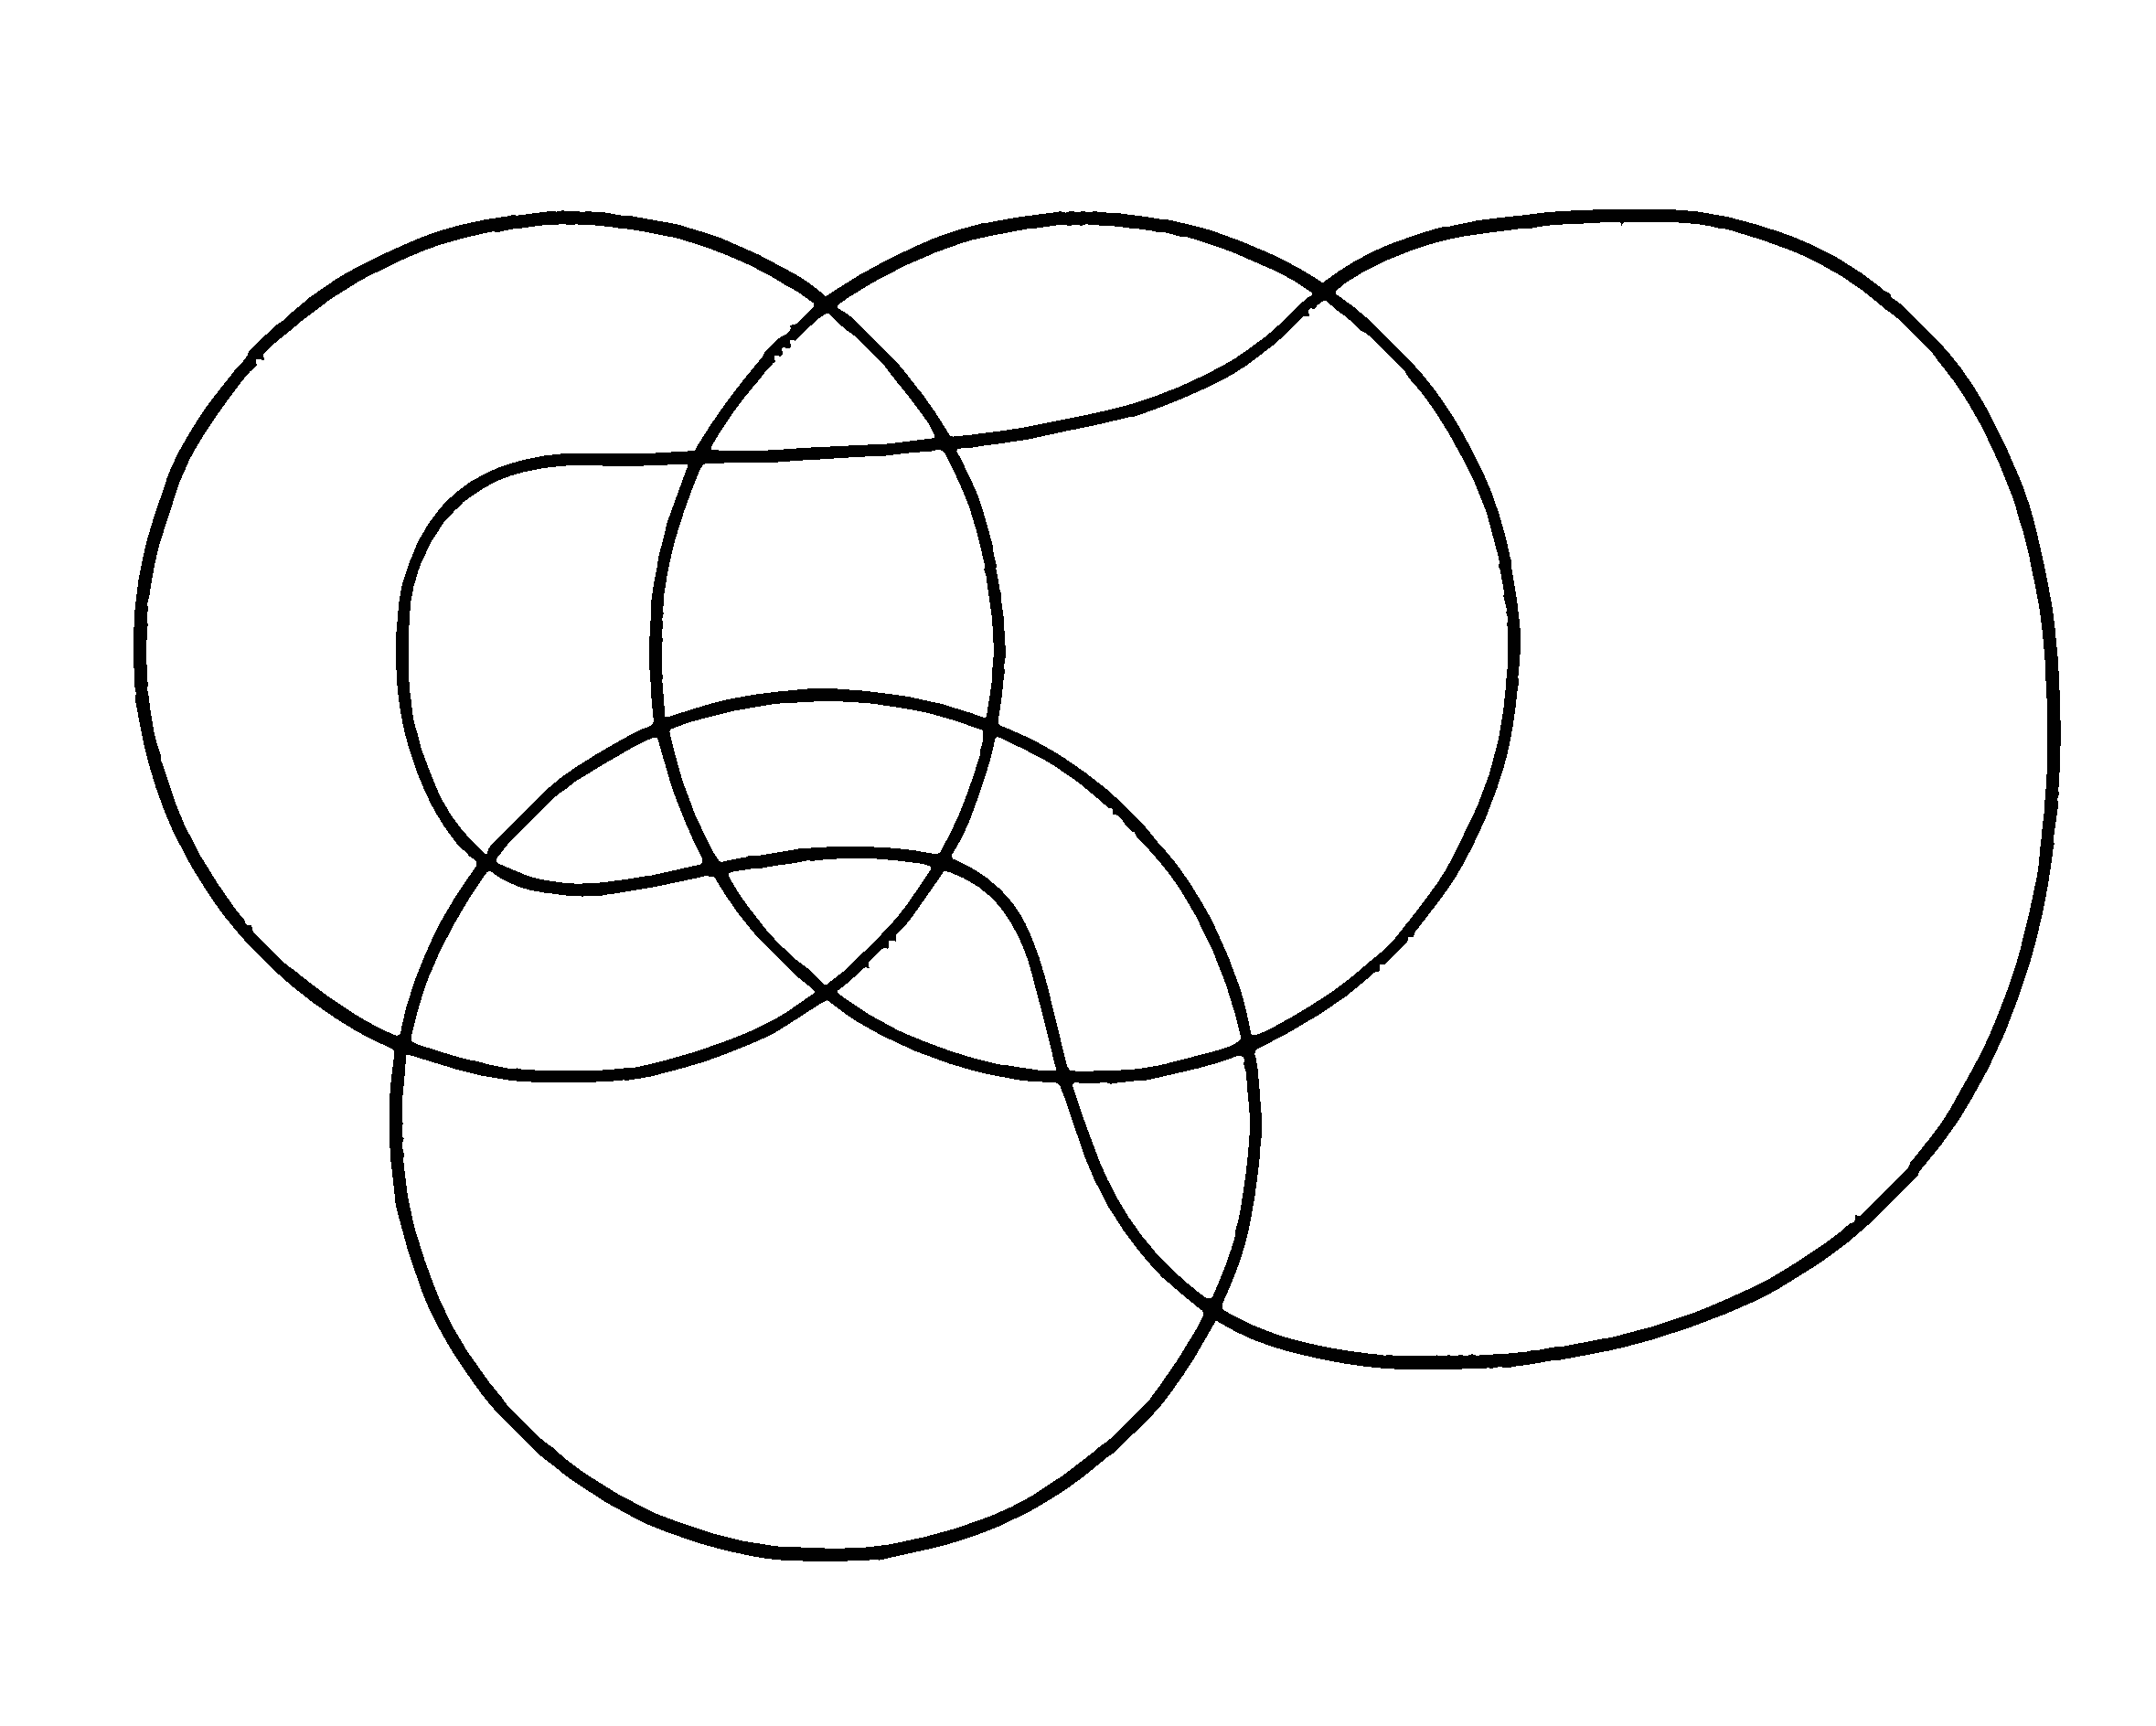
\includegraphics[width=10cm]{Images/MD.pdf}};
        \draw[ultra thick] (-6,-4) node[above right] {$(t = 4)$} rectangle (6,4);
        %\draw (-6,-4) grid (6,4);
        %\filldraw (0,0) circle (2.5pt);
        \node at (-5,2.5) {$1$};
        \node at (-3,2.5) {$2$};
        \node at (0,2.5) {$3$};
        \node at (3,-1) {$4$};
        \node at (-1.5,-2) {$5$};
        \node at (-1.2,2.2) {$6$};
        \node at (-2,-0.5) {$7$};
        \node at (-2.5,1) {$8$};
        \node at (1,1) {$9$};
        \node at (-0.5,-0.5) {$10$};
        \node at (0.45,-1.4) {$11$};
        \node at (-1.2,1.3) {$12$};
        \node at (-2.1,0.25) {$13$};
        \node at (0.1,-0.1) {$14$};
        \node at (-1.2,-0.2) {$15$};
        \node at (-1.2,0.4) {$16$};
        \node[below] at (-1.1,-3.3) {$c_1$};
        \node[above] at (-2.5,3) {$c_2$};
        \node[above] at (0,3) {$c_3$};
        \node[above] at (2.5,3) {$c_4$};
    \end{tikzpicture}
    \caption{~}\label{UAJSBSNZSKKS}
    \end{figure}
\end{itemize}

\begin{BOX}
    Si tomamos un elemento de la región 3, encontramos que se cuenta una vez en $E_1$ y una vez en $S_1$ [en $N\left(c_3\right)$]. Si tomamos un elemento de la región 6, vemos que no se cuenta en $E_1$; se cuenta dos veces en $S_1$ [en $N\left(c_2\right)$ y en $N\left(c_3\right)$] pero se elimina dos veces en $2 S_2$ [ya que se cuenta una vez en $S_2$ en $N\left(c_2 c_3\right)$], por lo que al final no cuenta. El lector debería examinar ahora un elemento de la región 12 y uno de la región 16 y mostrar que cada uno contribuye en 0 a ambos lados de la fórmula para $E_1$.
\end{BOX}

\begin{itemize}[resume]
    \item $E_2$ [regiones 6-11]: De la figura \ref{UAJSBSNZSKKS}, $\displaystyle E_2=S_2-3 S_3+6 S_4=S_2- \binom{3}{1}S_3 + \binom{4}{2} S_4$. Para más detalles sobre esta formula, examinemos los resultados que aparecen en la tabla \ref{JAJABBVVAHXXFTUQOP}, donde junto a cada sumando de $S_2, S_3$ y $S_4$ enumeramos las regiones cuyos elementos se cuentan para determinar ese sumando en particular. Para calcular $S_2-3 S_3+6 S_4$, encontramos los elementos de las regiones 6 a 11, que son precisamente los que se cuentan para $E_2$.
    \begin{center}
        \begin{NiceTabular}[hvlines-except-borders,rules={color=white,width=1pt}]{lll}
        \CodeBefore
        \rowcolor{jblueleft!80}{1}
        \rowcolors{2}{DodgerBlue3!40}{jblueinner}
        \Body
        \RowStyle[color=white]{}
            $S_2$ & $S_3$ & $S_4$ \\
            $N(c_1 c_2)$: 7, 13, 15, 16 & $N(c_1c_2c_3)$: 15, 16 & $N(c_1c_2c_3c_4)$: 16 \\
            $N(c_1 c_3)$: 10, 14, 15, 16 & $N(c_1c_2c_4)$: 13, 16 & \\
            $N(c_1 c_4)$: 11, 13, 14, 16 & $N(c_1c_2c_3)$: 14, 16 & \\
            $N(c_2 c_3)$: 6, 12, 15, 16 & $N(c_2c_3c_4)$: 12, 16 & \\
            $N(c_2 c_4)$: 8, 12, 13, 16 & & \\
            $N(c_3 c_4)$: 9, 12, 14, 16 & & \\
        \end{NiceTabular}
        \captionof{table}{~}\label{JAJABBVVAHXXFTUQOP}
    \end{center}
    \item $E_3$: Por último, los elementos de $E_3$ se encuentra en las regiones 12 a 15 y $\displaystyle E_3 = S_3 - 4S_4 = S_3 - \binom{4}{1}S_4$; los elementos para $E_4$ son los de la región 16 y $E_4 = S_4$.
\end{itemize}

\part*{\vspace{-0.13cm}APÉNDICES}

\appendix

\chapterimage{blue25.jpeg} % Imagen de encabezado de capítulo
\chapterspaceabove{6.75cm} % Espacio en blanco desde la parte superior de la página hasta el título del capítulo en las páginas del capítulo
\chapterspacebelow{6.25cm} % Cantidad de espacio en blanco vertical desde el margen superior hasta el comienzo del texto en las páginas de los capítulos

%------------------------------------------------

\chapter{INDUCCIÓN MATEMÁTICA}\label{ch:induccion}

\tcbsidebyside[title=Blaise Pascal,
      sidebyside adapt=left,
      bicolor,
      colback=white,
      colbacklower=jblueinner,
      colframe=jblueleft,
      fonttitle=\bfseries,
      center title,
      fuzzy shadow = {0pt}{-3pt}{-0.5pt}{0.5pt}{black!35},
]{%
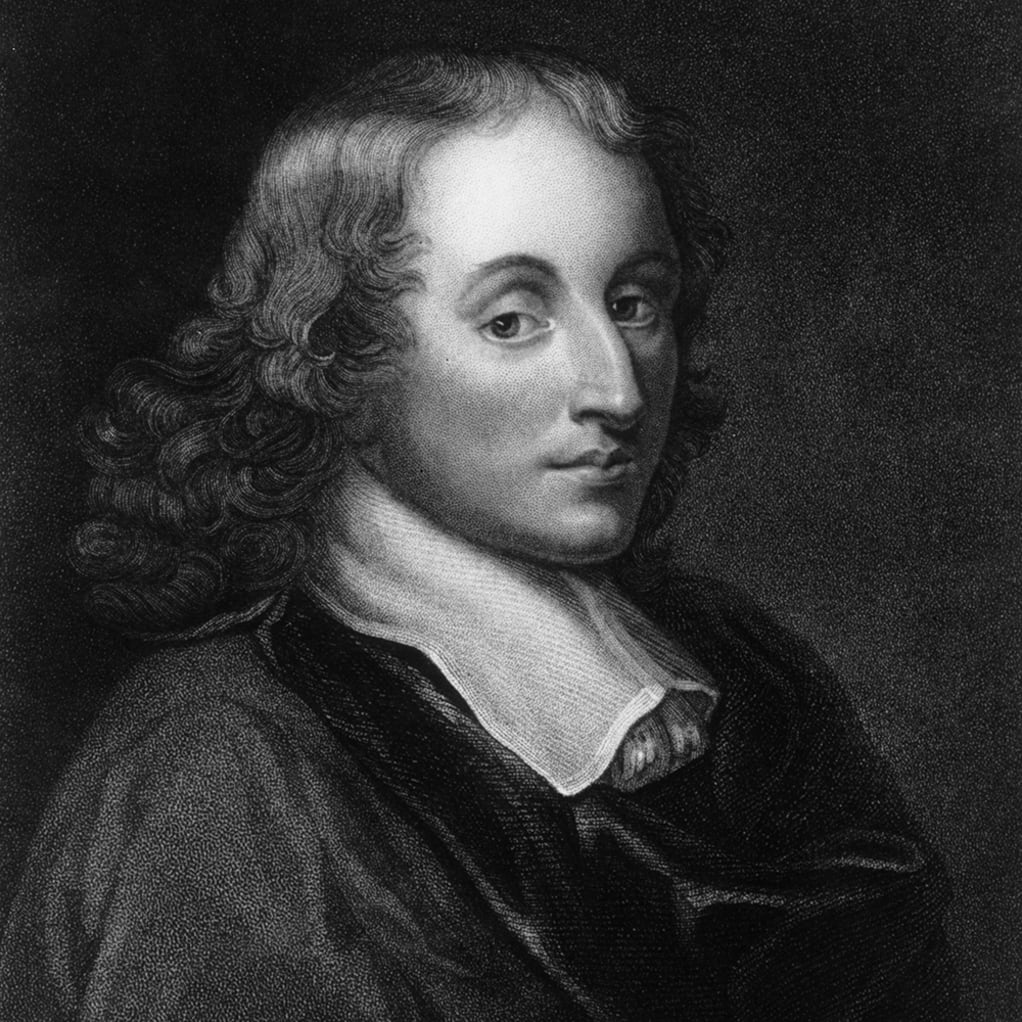
\includegraphics[width=0.36\textwidth]{PASCAL.jpeg}
}{%
    Nacido el 19 de junio de 1623 en Clermont-Ferrand, Francia; fue un genio precoz y de clara inteligencia, pues su entusiasmo juvenil por la ciencia se materializó en importantes y precursoras aportaciones a la física y a las matemáticas. Siendo aún niño, con solo doce años, sin ayuda alguna demostró que la suma de los ángulos de un triángulo es siempre igual a 180°. Su curiosidad lo llevo a que inventara la primera calculadora digital en 1642 (llamada \emph{Pascalina}) para ayudar a su padre, Étienne Pascal. Pese a su frágil salud y corta vida, murió a los treinta y nueve años, pero su huella quedó grabada en la historia de la física y de la informática.
}

%\section{Introducción}

\noindent
\begin{minipage}[c]{0.7\textwidth}
    Uno de los métodos más usados para realizar demostraciones es el Método de Inducción Matemática. Este fue creado por Blaise Pascal en el siglo XVII, aunque el primer matemático que ofreció una demostración formal mediante el uso explicito de la inducción matemática fue el italiano Franciscus Maurolicus (1494-1575). Maurolicus utilizo la inducción para demostrar que para todo entero positivo $n$
    \[1+3+5+\cdots +(2n-1)=n^2.\]
    Dicho método ha servido para demostrar teoremas en distintas áreas de la matemática; como: geometría, teoría de grafos, teoría de números, análisis combinatorio. Una manera informal (pero eficaz) de ver y explicar el Principio de Inducción Matemática es mediante fichas de dominó. Imaginemos que tenemos fichas de dominó puestas en una hilera infinita. Si empujamos la primer ficha, esta empujará la segunda ficha; la segunda ficha empujará la tercer ficha; la tercer ficha empujara la cuarta ficha; y así sucesivamente hasta que caigan \textbf{todas} las fichas. En este caso, cada ficha representa un número natural.
\end{minipage}
\begin{minipage}[c]{0.24\textwidth}
    \noindent
    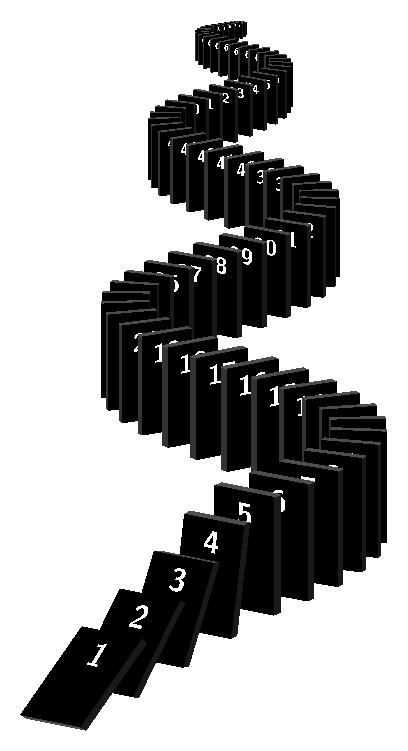
\includegraphics[width=1.17\textwidth]{uuu.pdf}
    %\captionof{figure}{Principio de Inducción}\label{fig:INDUCCION}
\end{minipage}

\newpage

\section{Principio de inducción}

\noindent
\textbf{\color{jblueleft}Problema:} Calcular la suma de los primeros $n$ números impares.\\
\,\\
Los problemas de este tipo se pueden resolver usando una fórmula probada. Pero nos interesa resolver el problema sin recurrir a tal fórmula y aplicando el método de la inducción matemática.
Para hacerlo, es necesario establecer primero una hipótesis, es decir, tratar simplemente de adivinar la solución.\\
\,\\
\textbf{\color{jblueleft}Solución:} Observemos las siguientes sumas parciales:
\begin{align*}
    1 &=1 \\
    1+3 &=4 \\
    1+3+5 &=9 \\
    1+3+5+7 &=16 \\
    1+3+5+7+9 &=25 \\
    1+3+5+7+9+11 &=36 \\
    & \vdots 
    %1+3+5+7+9+11+13 &=49 \\
    %1+3+5+7+9+11+13+15 &=64 %\\
    %1+3+5+7+9+11+13+15+17 &=81
\end{align*}
Cada suma puede representarse en la forma
$$\alpha + \beta + \gamma + \cdots + u = S,$$
donde $u$ representa el último sumando y $S$ la suma. Tanto $u$ como $S$ dependen del número de sumandos, al cual denominaremos con $n$. Dadas estas convenciones podemos hacer las tablas siguientes, y encontrar en la primera de ellas alguna relación entre $n$ y $u$; y en la segunda, alguna relación entre $n$ y $S$.
\begin{center}
    \begin{minipage}[c]{0.2\textwidth}
        \centering
        \begin{NiceTabular}[hvlines-except-borders,rules={color=white,width=1pt}]{cc}
        \CodeBefore
        \rowcolor{jblueleft!80}{1}
        \rowcolors{2}{DodgerBlue3!40}{jblueinner}
        \Body
        \RowStyle[color=white]{}
            $n$ & $u$ \\
            1 & 1 \\
            2 & 3 \\
            3 & 5 \\
            4 & 7 \\
            5 & 9 \\
            6 & 11
            %7 & 13 \\ \hline
            %8 & 15 \\ \hline
            %9 & 9 \\ \hline
        \end{NiceTabular}
    \end{minipage} \hspace{0.3cm}
    \begin{minipage}[c]{0.2\textwidth}
        \centering
        \begin{NiceTabular}[hvlines-except-borders,rules={color=white,width=1pt}]{cc}
        \CodeBefore
        \rowcolor{jblueleft!80}{1}
        \rowcolors{2}{DodgerBlue3!40}{jblueinner}
        \Body
        \RowStyle[color=white]{}
            $n$ & $S$ \\
            1 & 1 \\
            2 & 4 \\
            3 & 9 \\
            4 & 16 \\
            5 & 25 \\
            6 & 36
            %7 & 49 \\ \hline
            %8 & 64 \\ \hline
            %9 & 81 \\ \hline
        \end{NiceTabular}
    \end{minipage}
\end{center}
Por lo que se propone el siguiente modelo:
$$1+3+5+7+9+11+\cdots +(2n-1)=n^2.$$
Probemosla por medio de inducción sobre $n$. Llamemos a la suma, $S_n$. Es decir,
$$S_n=1+3+5+7+9+11+\cdots +(2n-1)$$
\begin{enumerate}[label=\roman*)]
    \item Para $n=1$ es evidente que se cumple, ya que la suma consiste en un solo término, el 1. El valor de la expresión $n^2$ también es 1.
    \item Supóngase que la hipótesis se cumple para $n=k$, es decir, $S_k=k^2$.
    \item A partir de (ii), probemos que se cumple para $n=k+1$, es decir,
    $$S_{k+1}=(k+1)^2.$$
    En efecto, se tiene
    $$S_{k+1}=S_k+(2k+1),$$
    pero $S_k=k^2$. Se sigue que
    $$S_{k+1}=k^2+(2k+1)=(k+1)^2.$$
\end{enumerate}
En conclusión, se cumple que $S_n=n^2$.\\
\newline
Incluso, para este caso, podemos ver la \emph{demostración visual}\footnote{Una demostración visual significa que la solución de dicho problema sea accesible mediante un diagrama o dibujo de forma evidente, sin apenas desarrollo matemático.} de
$$1+3+5+7+9+11+\cdots +(2n-1)=n^2.$$
Imaginemos que cada círculo equivale a una unidad. Entonces,
\begin{enumerate}
    \item Para $n=1$:
    \begin{center}
        \begin{tikzpicture}
            \filldraw[Turquoise1] (0,0) circle (0.25cm);
        \end{tikzpicture}
    \end{center}
    \item Para $n=2$:
    \begin{center}
        \begin{tikzpicture}
            \filldraw[Turquoise1] (0,0) circle (0.25cm);
            \filldraw[jblueleft] (1,0) circle (0.25cm);
            \filldraw[jblueleft] (1,1) circle (0.25cm);
            \filldraw[jblueleft] (0,1) circle (0.25cm);
        \end{tikzpicture}
    \end{center}
    \item Para $n=3$:
    \begin{center}
        \begin{tikzpicture}
            \filldraw[Turquoise1] (0,0) circle (0.25cm);
            \filldraw[jblueleft] (1,0) circle (0.25cm);
            \filldraw[jblueleft] (1,1) circle (0.25cm);
            \filldraw[jblueleft] (0,1) circle (0.25cm);
            \filldraw[SkyBlue1] (2,0) circle (0.25cm);
            \filldraw[SkyBlue1] (2,1) circle (0.25cm);
            \filldraw[SkyBlue1] (2,2) circle (0.25cm);
            \filldraw[SkyBlue1] (1,2) circle (0.25cm);
            \filldraw[SkyBlue1] (0,2) circle (0.25cm);
        \end{tikzpicture}
    \end{center}
    \item Para $n=4$:
    \begin{center}
        \begin{tikzpicture}
            \filldraw[Turquoise1] (0,0) circle (0.25cm);
            \filldraw[jblueleft] (1,0) circle (0.25cm);
            \filldraw[jblueleft] (1,1) circle (0.25cm);
            \filldraw[jblueleft] (0,1) circle (0.25cm);
            \filldraw[SkyBlue1] (2,0) circle (0.25cm);
            \filldraw[SkyBlue1] (2,1) circle (0.25cm);
            \filldraw[SkyBlue1] (2,2) circle (0.25cm);
            \filldraw[SkyBlue1] (1,2) circle (0.25cm);
            \filldraw[SkyBlue1] (0,2) circle (0.25cm);
            \filldraw[RoyalBlue1] (3,0) circle (0.25cm);
            \filldraw[RoyalBlue1] (3,1) circle (0.25cm);
            \filldraw[RoyalBlue1] (3,2) circle (0.25cm);
            \filldraw[RoyalBlue1] (3,3) circle (0.25cm);
            \filldraw[RoyalBlue1] (2,3) circle (0.25cm);
            \filldraw[RoyalBlue1] (1,3) circle (0.25cm);
            \filldraw[RoyalBlue1] (0,3) circle (0.25cm);
        \end{tikzpicture}
    \end{center}
\end{enumerate}
Recordemos que esto es una manera visual de ver el comportamiento de una proposición particular. Pero no siempre se puede recurrir a una demostración visual, ya que nos puede llevar a conclusiones falsas.

\newpage

\begin{tcolorbox}[
      theorem style=change break,
      enhanced,
      breakable,
      boxrule=0pt,
      frame hidden,
      borderline west={3pt}{0pt}{jblueleft},
      colback=jblueinner,
      coltitle=jblueleft,
      attach title to upper={\ },
      sharp corners,
      title={Principio de inducción matemática:},
      fonttitle=\bfseries,
      fontupper=\normalsize
]
    Sea $P$ una propiedad cualquiera. Tenemos que $P(1)$, $P(2)$, $P(3)$, $P(4)$, $\dots$ es un conjunto de propiedades para cada número natural tal que:
    \begin{enumerate}[label=\roman*)]
        \item $P(1)$ es cierta.
        \item Si $P(n)$ es cierta, entonces $P(n+1)$ es cierta.
    \end{enumerate}
    Entonces $P(n)$ es cierta para toda $n \in \mathbb{N}$.
\end{tcolorbox}

\begin{BOX}
    A la suposición de que la propiedad es cierta para $n$ se le conoce como \textbf{hipótesis de inducción} o \textbf{hipótesis inductiva}.
\end{BOX}

\begin{myexample}
    Demostrar que
    $$1+2+\cdots +n=\frac{n(n+1)}{2}, \,\, \forall n \in \mathbb{N}.$$
    
    \tcblower
    \textbf{\color{jblueleft}Demostración:}
    \begin{enumerate}[label=\roman*)]
        \item Claramente $n=1$, satisface la fórmula, ya que
        \begin{align*}
            1 &=\frac{1(1+1)}{2} \\
            1 &=1
        \end{align*}
        \item Supongamos que la fórmula se cumple para $n=k$, es decir, supongamos que
        $$1+2+\cdots +k=\frac{k(k+1)}{2}.$$
        Demostraremos a partir de lo dicho anteriormente que la fórmula se cumple para $n=k+1$. Es decir, probaremos que
        $$1+2+\cdots +k=\frac{(k+1)(k+2)}{2}.$$
        En efecto, por hipótesis de inducción
        $$1+2+\cdots +k=\frac{k(k+1)}{2}.$$
        Entonces
        \begin{align*}
            1+2+\cdots +k+k+1 &=\frac{k(k+1)}{2}+k+1 \\
            &=\frac{k(k+1)+2(k+1)}{2} \\
            &=\frac{(k+1)(k+2)}{2}
        \end{align*}
        es decir,
        $$1+2+\cdots +k+1=\frac{(k+1)(k+2)}{2}$$
    \end{enumerate}
    Por tanto,
    $$1+2+\cdots +n=\frac{n(n+1)}{2}, \,\, \forall n \in \mathbb{N}.$$
\end{myexample}

\begin{BOX}
    Del ejemplo anterior, si utilizamos la notación suma, tenemos:
    $$\sum_{i=1}^n i = 1+2+\cdots +n = \frac{n(n+1)}{2}, \,\, \forall n \in \mathbb{N}.$$
\end{BOX}

\begin{myexample}\label{EX:APUDJSKS}
    Demostrar que
    $$1^2+2^2+\cdots +n^2=\frac{n(n+1)(2n+1)}{6}, \,\, \forall n \in \mathbb{N}.$$
    \tcblower
    \textbf{\color{jblueleft}Demostración:}
    \begin{enumerate}[label=\roman*)]
        \item Claramente $n=1$ satisface la fórmula, ya que al sustituir $n$ por 1 se tiene
        \begin{align*}
            1^2 &=\frac{1(1+1)(2\cdot 1+1)}{6} \\
            1 &=1
        \end{align*}
        lo cual es verdadero.
        \item Supongamos que la fórmula se cumple para $n=k$, es decir, supongamos que
        $$1^2+2^2+\cdots +k^2=\frac{k(k+1)(2k+1)}{6}.$$
        Demostraremos a partir de lo dicho anteriormente que la fórmula se cumple para $n=k+1$. Es decir, probaremos que
        $$1^2+2^2+\cdots +(k+1)^2=\frac{(k+1)(k+2)(2k+3)}{6}.$$
        En efecto: por hipótesis de inducción
        $$1^2+2^2+\cdots +k^2=\frac{k(k+1)(2k+1)}{6}.$$
        Entonces
        \begin{align*}
            1^2 +2^2+\cdots +k^2+(k+1)^2 &=\frac{k(k+1)(2k+1)}{6}+(k+1)^2 \\
            &=\frac{k(k+1)(2k+1)+6(k+1)^2}{6} \\
            &=\frac{(k+1)\big(k(2k+1)+6(k+1)\big)}{6} \\
            &=\frac{(k+1)(2k^2+7k+6)}{6} \\
            &=\frac{(k+1)(k+2)(2k+3)}{6}
        \end{align*}
    \end{enumerate}
    Por tanto,
    $$1^2+2^2+\cdots +n^2=\frac{n(n+1)(2n+1)}{6}, \, \forall n \in \mathbb{N}.$$
\end{myexample}

\newpage

\begin{BOX}
    Del ejemplo anterior, si utilizamos la notación suma, tenemos:
    $$\sum_{i=1}^n i^2 = 1^2+2^2+\cdots +n^2=\frac{n(n+1)(2n+1)}{6}, \, \forall n \in \mathbb{N}.$$
\end{BOX}

\begin{importante}
    El método de la inducción matemática no es el único procedimiento para demostrar que una propiedad $P$ se cumple para cada número natural.
\end{importante}

\begin{BOX}
    En resumen, cuando se quiere demostrar que una propiedad $P$ se cumple para cada número natural, se emplea un procedimiento llamado \textbf{demostración por inducción matemática}. Es decir, si $\mathbb{N}$ es el conjunto de los números naturales y $A \subset \mathbb{N}$ tal que:
    \begin{enumerate}[label=\roman*)]
        \item $1 \in A$.
        \item $k \in A \Longrightarrow k+1 \in A$. Entonces $A=\mathbb{N}$
    \end{enumerate}
\end{BOX}

\begin{importante}
    Si no se puede demostrar que una propiedad $P$ se cumple para cada número natural, no significa que $P$ sea falsa, sino solamente que no se ha podido hacer la demostración. Una manera de demostrar que $P$ es falsa sería dar un \textbf{contraejemplo}.
\end{importante}

\begin{myexample}
    Consideremos el polinomio $f(x)=x^2+x+41$. Si este polinomio se remplaza $x$ por el número 0, se obtiene el número primo 41. Si se remplaza $x$ por el número 1, nuevamente se obtiene un número primo, 43. Si se sigue este procedimiento para 1, 2, 3, 4, 5, 6, 7, 8, 9; obtenemos que
    \begin{align*}
        f(0) &=41 \\
        f(1) &=43 \\
        f(2) &=47 \\
        f(3) &=53 \\
        f(4) &=61 \\
        f(5) &=71 \\
        f(6) &=83 \\
        f(7) &=97 \\
        f(8) &=113 \\
        f(9) &=131
    \end{align*}
    Basándonos en estos resultados podríamos concluir que para todo entero no negativo $x$, el valor del polinomio es un número primo. Pero esto no es así, pues el polinomio $x^2+x+41$ produce números primos para $f(0), \, f(1), \, f(2), \, f(3), \, \dots, \, f(38), \, f(39)$ y al obtener el resultado de $f(40)$, que es $1681$, vemos que es un número compuesto.
\end{myexample}

\newpage

\begin{myexample}
    Demuestre el teorema del binomio. Es decir, $\displaystyle (a+b)^n=\sum_{r=0}^{n}\binom{n}{r}a^{n-r}b^r$.
    
    \tcblower
    \textbf{\color{jblueleft}Demostración:}
    \begin{enumerate}[label=\roman*)]
        \item Si $n=1$, entonces
        \begin{align*}
            \sum_{r=0}^{1}\binom{1}{r}a^{1-r}b^r &= \binom{1}{0} a^{1-0}b^0 + \binom{1}{1} a^{1-1}b^1 \\
            &=a+b
        \end{align*}
        \item Supongamos que se cumple para $n=k$, es decir, supongamos que
        $$(a+b)^k=\sum_{r=0}^{k}\binom{k}{r}a^{k-r}b^r.$$
        Demostraremos a partir de lo dicho anteriormente, que la propiedad se cumple para $n=k+1$, es decir,
        $$(a+b)^{k+1} = \sum_{r=0}^{k+1}\binom{k+1}{r}a^{k+1-r}b^r.$$
        Entonces
        \begin{align*}
            (a+b)^{k+1} &=(a+b)(a+b)^k \\
            &=(a+b) \sum_{r=0}^{k} \binom{k}{r} a^{k-r}b^r \\
            &=a\sum_{r=0}^{k} \binom{k}{r} a^{k-r}b^r + b \sum_{r=0}^{k} \binom{k}{r} a^{k-r}b^r \\
            &=\sum_{r=0}^{k} \binom{k}{r} a^{k+1-r}b^r +  \sum_{r=0}^{k} \binom{k}{r} a^{k-r}b^{r+1} \\
            &=\sum_{r=0}^{k} \binom{k}{r} a^{k+1-r}b^r +  \sum_{r=0}^{k} \binom{k}{r-1} a^{k-(r-1)}b^{r-1+1} \\
            &=\binom{k}{0} a^{k+1} + \sum_{r=1}^{k} \binom{k}{r} a^{k+1-r}b^r + \sum_{r=1}^{k} \binom{k}{r-1} a^{k-r+1}b^r \\
            &= a^{k+1} + \sum_{r=1}^{k} \left[ \binom{k}{r}+\binom{k}{r-1} \right] a^{k+1-r}b^r \\
            &=a^{k+1}+\sum_{r=1}^{k} \binom{k+1}{r} a^{k+1-r} b^r \\
            &=\binom{k+1}{0}a^{k+1-0}b^0+\sum_{r=1}^{k} \binom{k+1}{r} a^{k+1-r}b^r \\
            &=\sum_{r=0}^{k+1} \binom{k+1}{r}a^{k+1-r}b^r
        \end{align*}
    \end{enumerate}
\end{myexample}

\newpage

\begin{myexample}
    Hallar una expresión para la suma
    $$1 \cdot 1! + 2 \cdot 2! + 3 \cdot 3! + \cdots + n \cdot n!.$$
    
    \tcblower
    \textbf{\color{jblueleft}Solución:} Llamemos a la suma anterior, $S_n$. Es decir
    $$S_n=1 \cdot 1! + 2 \cdot 2! + 3 \cdot 3! + \cdots + n \cdot n!.$$
    Veamos las siguientes sumas
    \begin{align*}
        1 \cdot 1! &=1 \\
        1 \cdot 1!+2 \cdot 2! &=5 \\
        1 \cdot 1!+2 \cdot 2! + 3 \cdot 3! &=23 \\
        1 \cdot 1!+2 \cdot 2! + 3 \cdot 3! +4 \cdot 4! &=119 \\
        1 \cdot 1!+2 \cdot 2! + 3 \cdot 3! +4 \cdot 4! +5 \cdot 5! &=719 \\
        & \vdots
    \end{align*}
    Examinando las anteriores sumas, se observa que
    \begin{align*}
        S_1 &=2!-1 \\
        S_2 &=3!-1 \\
        S_3 &=4!-1 \\
        S_4 &=5!-1 \\
        S_5 &=6!-1 \\
        & \vdots
    \end{align*}
    Esto conduce a la hipótesis
    $$S_n=(n+1)!-1.$$
    Verifiquemos dicha hipótesis.
    \begin{enumerate}[label=\roman*)]
        \item La hipótesis se cumple para $n=1$, pues
        $$S_1=1 \cdot 1!=2!-1.$$
        \item Supongamos que la hipótesis se cumple para $n=k$, es decir,
        $$S_k=(k+1)!-1.$$
        En efecto,
        \begin{align*}
            S_{k+1} &= S_k + (k+1) \cdot (k+1)! \\
            &=[(k+1)!-1]+(k+1) \cdot (k+1)! \\
            &=(k+1)![1+(k+1)]-1 \\
            &=(k+1)!(k+2)-1 \\
            &=(k+2)!-1
        \end{align*}
    \end{enumerate}
\end{myexample}

\chapterimage{blue19.jpeg} % Imagen de encabezado de capítulo
\chapterspaceabove{6.75cm} % Espacio en blanco desde la parte superior de la página hasta el título del capítulo en las páginas del capítulo
\chapterspacebelow{7.25cm} % Cantidad de espacio en blanco vertical desde el margen superior hasta el comienzo del texto en las páginas de los capítulos

%------------------------------------------------

\chapter{EL USO DE LA COMPUTADORA}


La computadora es una herramienta fundamental en la sociedad actual y tiene una amplia gama de aplicaciones en diversos campos, desde el ámbito empresarial y científico hasta el entretenimiento y la comunicación. El uso de la computadora ha revolucionado la forma en que trabajamos, nos comunicamos y nos entretenemos.



Uno de los aspectos clave en el uso de las computadoras es la programación. Los lenguajes de programación son conjuntos de instrucciones que permiten a los desarrolladores comunicarse con las computadoras y crear software y aplicaciones. Existen muchos lenguajes de programación diferentes, cada uno con sus propias características y aplicaciones específicas. Algunos de los lenguajes de programación más populares incluyen:
\begin{enumerate}
\item Python: Es un lenguaje de programación versátil y fácil de aprender, que se utiliza ampliamente en campos como la ciencia de datos, la inteligencia artificial y el desarrollo web.
\item Java: Es un lenguaje de programación de propósito general que se utiliza en una amplia variedad de aplicaciones, desde aplicaciones empresariales hasta desarrollo de Android.
\item C++: Es un lenguaje de programación de bajo nivel que se utiliza en el desarrollo de sistemas, juegos y aplicaciones de alto rendimiento.
\item JavaScript: Es un lenguaje de programación que se utiliza principalmente para desarrollar aplicaciones web interactivas y dinámicas.
%\item Ruby: Es un lenguaje de programación conocido por su elegancia y facilidad de lectura, utilizado principalmente en el desarrollo web.
\item C\#: Es un lenguaje de programación desarrollado por Microsoft, utilizado principalmente en el desarrollo de aplicaciones de Windows y juegos de Unity.
\item PHP: Es un lenguaje de programación utilizado principalmente en el desarrollo de aplicaciones web y la creación de sitios dinámicos.
\end{enumerate}


Estos son solo algunos ejemplos, y existen muchos otros lenguajes de programación disponibles, cada uno con sus propias ventajas y desventajas. La elección del lenguaje de programación dependerá de los requisitos del proyecto, las preferencias del desarrollador y las características específicas que se necesiten. Considerando que las computadoras son herramientas muy importantes en nuestra actualidad, particularmente, para ahorrarnos tiempo y esfuerzo en el trabajo de calcular, proporcionaremos algunos programas escritos en lenguaje C++, para hacer el cálculo que en cada caso se indica.

\newpage

\section*{Programa para evaluar un número en la función suelo y techo}

\noindent
\begin{lstlisting}[language=C++]
#include <iostream>
#include <cstdlib>
#include <locale.h>
#include <cmath>

int main() {
    double numero;
    std::cout << "Introduce un numero real: ";
    std::cin >> numero;

    double suelo = floor(numero);
    double techo = ceil(numero);

    std::cout << "El suelo de " << numero << " es: " << suelo << std::endl;
    std::cout << "El techo de " << numero << " es: " << techo << std::endl;

    system ("pause>null");
    return 0;
}
\end{lstlisting}

\section*{Programa que calcula las raíces de una ecuación de segundo grado}

\noindent
\begin{lstlisting}[language=C++]
#include <iostream>
#include <cstdlib>
#include <locale.h>
#include <cmath>

int main() {
    setlocale(LC_ALL, "");
    double a, b, c;
    double discriminante, raiz1, raiz2;

    std::cout << "Ingrese los coeficientes de la ecuacion de segundo grado:" << std::endl;
    std::cout << "a: ";
    std::cin >> a;
    std::cout << "b: ";
    std::cin >> b;
    std::cout << "c: ";
    std::cin >> c;

    discriminante = b * b - 4 * a * c;

    if (discriminante > 0) {
        raiz1 = (-b + sqrt(discriminante)) / (2 * a);
        raiz2 = (-b - sqrt(discriminante)) / (2 * a);

        std::cout << "Las raices son reales y diferentes:" << std::endl;
        std::cout << "Raiz 1: " << raiz1 << std::endl;
        std::cout << "Raiz 2: " << raiz2 << std::endl;
    } else if (discriminante == 0) {
        raiz1 = -b / (2 * a);

        std::cout << "Las raices son reales e iguales:" << std::endl;
        std::cout << "Raiz: " << raiz1 << std::endl;
    } else {
        double parteReal = -b / (2 * a);
        double parteImaginaria = sqrt(-discriminante) / (2 * a);

        std::cout << "Las raices son complejas conjugadas:" << std::endl;
        std::cout << "Raiz 1: " << parteReal << " + " << parteImaginaria << "i" << std::endl;
        std::cout << "Raiz 2: " << parteReal << " - " << parteImaginaria << "i" << std::endl;
    }

	system ("pause>null");
	return 0;
}

\end{lstlisting}

\section*{Programa que calcula la suma de los primeros $\bm{n}$ números naturales}

\noindent
\begin{lstlisting}[language=C++]
#include <iostream>
#include <cstdlib>
#include <locale.h>

int main() {
    setlocale(LC_ALL, "");
    int n;
    int suma = 0;

    std::cout << "Ingrese el valor de N: ";
    std::cin >> n;

    for (int i = 1; i <= n; i++) {
        suma += i;
    }

    std::cout << "La suma de los " << n << " primeros numeros naturales es: " << suma << std::endl;

	system ("pause>null");
	return 0;
}

\end{lstlisting}

\section*{Programa que calcula la suma de los primeros $\bm{n}$ números pares}

\noindent
\begin{lstlisting}[language=C++]
#include <iostream>
#include <cstdlib>
#include <locale.h>

int main() {
    setlocale(LC_ALL, "");
    int n;
    int suma = 0;

    std::cout << "Ingrese el valor de N: ";
    std::cin >> n;

    for (int i = 2; i <= n * 2; i += 2) {
        suma += i;
    }

    std::cout << "La suma de los " << n << " primeros numeros pares es: " << suma << std::endl;

	system ("pause>null");
	return 0;
}

\end{lstlisting}

\section*{Programa que verifica si un número es primo}

\noindent
\begin{lstlisting}[language=C++]
#include <iostream>
#include <cstdlib>
#include <locale.h>

bool esPrimo(int numero) {
    if (numero <= 1) {
        return false;
    }

    for (int i = 2; i * i <= numero; i++) {
        if (numero % i == 0) {
            return false;
        }
    }

    return true;
}

int main() {
    setlocale(LC_ALL, "");
    int numero;

    std::cout << "Ingrese un numero: ";
    std::cin >> numero;

    if (esPrimo(numero)) {
        std::cout << numero << " es un numero primo." << std::endl;
    } else {
        std::cout << numero << " no es un numero primo." << std::endl;
    }

	system ("pause>null");
	return 0;
}

\end{lstlisting}

\section*{Programa que calcula el MCD de dos números enteros}

\noindent
\begin{lstlisting}[language=C++]
#include <iostream>
#include <cstdlib>
#include <locale.h>

int calcularMCD(int num1, int num2) {
    while (num2 != 0) {
        int temp = num2;
        num2 = num1 % num2;
        num1 = temp;
    }

    return num1;
}

int main() {
    setlocale(LC_ALL, "");
    int num1, num2;

    std::cout << "Ingrese el primer numero: ";
    std::cin >> num1;

    std::cout << "Ingrese el segundo numero: ";
    std::cin >> num2;

    int mcd = calcularMCD(num1, num2);

    std::cout << "El Maximo Comun Divisor (MCD) de " << num1 << " y " << num2 << " es: " << mcd << std::endl;

	system ("pause>null");
	return 0;
}

\end{lstlisting}

\section*{Programa que suma dos matrices}

\noindent
\begin{lstlisting}[language=C++]
#include <iostream>
#include <cstdlib>
#include <locale.h>

const int MAX_FILAS = 100;
const int MAX_COLUMNAS = 100;

void sumarMatrices(int matriz1[][MAX_COLUMNAS], int matriz2[][MAX_COLUMNAS], int resultado[][MAX_COLUMNAS], int filas, int columnas) {
    for (int i = 0; i < filas; i++) {
        for (int j = 0; j < columnas; j++) {
            resultado[i][j] = matriz1[i][j] + matriz2[i][j];
        }
    }
}

int main() {
    setlocale(LC_ALL, "");
    int filas, columnas;
    int matriz1[MAX_FILAS][MAX_COLUMNAS];
    int matriz2[MAX_FILAS][MAX_COLUMNAS];
    int resultado[MAX_FILAS][MAX_COLUMNAS];

    std::cout << "Ingrese el numero de filas: ";
    std::cin >> filas;
    std::cout << "Ingrese el numero de columnas: ";
    std::cin >> columnas;

    std::cout << "Ingrese los elementos de la matriz 1:" << std::endl;
    for (int i = 0; i < filas; i++) {
        for (int j = 0; j < columnas; j++) {
            std::cout << "Ingrese el elemento " << i+1 << "," << j+1 << ": ";
            std::cin >> matriz1[i][j];
        }
    }

    std::cout << "Ingrese los elementos de la matriz 2:" << std::endl;
    for (int i = 0; i < filas; i++) {
        for (int j = 0; j < columnas; j++) {
            std::cout << "Ingrese el elemento " << i+1 << "," << j+1 << ": ";
            std::cin >> matriz2[i][j];
        }
    }

    sumarMatrices(matriz1, matriz2, resultado, filas, columnas);

    std::cout << "La matriz resultado es:" << std::endl;
    for (int i = 0; i < filas; i++) {
        for (int j = 0; j < columnas; j++) {
            std::cout << resultado[i][j] << " ";
        }
        std::cout << std::endl;
    }

	system ("pause>null");
	return 0;
}

\end{lstlisting}

\section*{Programa que multiplica dos matrices}

\noindent
\begin{lstlisting}[language=C++]
#include <iostream>
#include <cstdlib>
#include <locale.h>

const int MAX_FILAS = 100;
const int MAX_COLUMNAS = 100;

void multiplicarMatrices(int matriz1[][MAX_COLUMNAS], int matriz2[][MAX_COLUMNAS], int resultado[][MAX_COLUMNAS], int filas1, int columnas1, int columnas2) {
    for (int i = 0; i < filas1; i++) {
        for (int j = 0; j < columnas2; j++) {
            resultado[i][j] = 0;
            for (int k = 0; k < columnas1; k++) {
                resultado[i][j] += matriz1[i][k] * matriz2[k][j];
            }
        }
    }
}

int main() {
    setlocale(LC_ALL, "");
    int filas1, columnas1, filas2, columnas2;
    int matriz1[MAX_FILAS][MAX_COLUMNAS];
    int matriz2[MAX_FILAS][MAX_COLUMNAS];
    int resultado[MAX_FILAS][MAX_COLUMNAS];

    std::cout << "Ingrese el numero de filas de la matriz 1: ";
    std::cin >> filas1;
    std::cout << "Ingrese el numero de columnas de la matriz 1: ";
    std::cin >> columnas1;
    std::cout << "Ingrese el numero de filas de la matriz 2: ";
    std::cin >> filas2;
    std::cout << "Ingrese el numero de columnas de la matriz 2: ";
    std::cin >> columnas2;

    if (columnas1 != filas2) {
        std::cout << "Error: Las matrices no se pueden multiplicar." << std::endl;
        return 0;
    }

    std::cout << "Ingrese los elementos de la matriz 1:" << std::endl;
    for (int i = 0; i < filas1; i++) {
        for (int j = 0; j < columnas1; j++) {
            std::cout << "Ingrese el elemento " << i+1 << "," << j+1 << ": ";
            std::cin >> matriz1[i][j];
        }
    }

    std::cout << "Ingrese los elementos de la matriz 2:" << std::endl;
    for (int i = 0; i < filas2; i++) {
        for (int j = 0; j < columnas2; j++) {
            std::cout << "Ingrese el elemento " << i+1 << "," << j+1 << ": ";
            std::cin >> matriz2[i][j];
        }
    }

    multiplicarMatrices(matriz1, matriz2, resultado, filas1, columnas1, columnas2);

    std::cout << "La matriz resultante es:" << std::endl;
    for (int i = 0; i < filas1; i++) {
        for (int j = 0; j < columnas2; j++) {
            std::cout << resultado[i][j] << " ";
        }
        std::cout << std::endl;
    }

	system ("pause>null");
	return 0;
}

\end{lstlisting}

%\newpage

\section*{Programa que calcula la transpuesta de una matriz}

\noindent
\begin{lstlisting}[language=C++]
#include <iostream>
#include <cstdlib>
#include <locale.h>

const int MAX_FILAS = 100;
const int MAX_COLUMNAS = 100;

void obtenerMatrizTranspuesta(int matriz[MAX_FILAS][MAX_COLUMNAS], int filas, int columnas, int matrizTranspuesta[MAX_COLUMNAS][MAX_FILAS]) {
    for (int i = 0; i < filas; i++) {
        for (int j = 0; j < columnas; j++) {
            matrizTranspuesta[j][i] = matriz[i][j];
        }
    }
}

void mostrarMatriz(int matriz[MAX_FILAS][MAX_COLUMNAS], int filas, int columnas) {
    for (int i = 0; i < filas; i++) {
        for (int j = 0; j < columnas; j++) {
            std::cout << matriz[i][j] << " ";
        }
        std::cout << std::endl;
    }
}

int main() {
    setlocale(LC_ALL, "");
    int filas, columnas;
    int matriz[MAX_FILAS][MAX_COLUMNAS];
    int matrizTranspuesta[MAX_COLUMNAS][MAX_FILAS];

    std::cout << "Ingrese el numero de filas de la matriz: ";
    std::cin >> filas;
    std::cout << "Ingrese el numero de columnas de la matriz: ";
    std::cin >> columnas;

    std::cout << "Ingrese los elementos de la matriz:" << std::endl;
    for (int i = 0; i < filas; i++) {
        for (int j = 0; j < columnas; j++) {
            std::cin >> matriz[i][j];
        }
    }

    obtenerMatrizTranspuesta(matriz, filas, columnas, matrizTranspuesta);

    std::cout << "Matriz original:" << std::endl;
    mostrarMatriz(matriz, filas, columnas);

    std::cout << "Matriz transpuesta:" << std::endl;
    mostrarMatriz(matrizTranspuesta, columnas, filas);

	system ("pause>null");
	return 0;
}

\end{lstlisting}

\chapterimage{blue26.jpeg} % Imagen de encabezado de capítulo
\chapterspaceabove{6.75cm} % Espacio en blanco desde la parte superior de la página hasta el título del capítulo en las páginas del capítulo
\chapterspacebelow{7.25cm} % Cantidad de espacio en blanco vertical desde el margen superior hasta el comienzo del texto en las páginas de los capítulos

\chapter*{BIBLIOGRAFÍA}

\section*{Fuente básica}

\begin{enumerate}[label={[\arabic*]}]
    \item Grimaldi, R. P. (1998). Matemáticas Discretas y Combinatoria: Una introducción con aplicaciones (3a. ed., 3a. reimp.). México: Addison-Wesley Iberoamericana\footnote{Aunque existen tres fuentes básicas, para esta obra usaremos principalmente esta fuente.}.
    \item Robert R. Korfhage (1970). Lógica y Algoritmos. Limusa Wiley.
    \item Kenneth H. Rosen (1991). Discrete Mathematics and its applications (2a. ed.). McGraw-Hill.
\end{enumerate}

\section*{Fuente de consulta}

\begin{enumerate}[resume,label={[\arabic*]}]
    \item Abraham P. Hillman-Gerald L. Alexanderson-Richar M. Grass (1990). Discrete and Combinational Mathematics. Cullier Macmillan.
    \item McEliece-ASH (1989). Introduction to Discrete Mathematics. Rndom-House.
    \item Mauer-Ralston (1991). Discrete Algorithmic Mathematics. Addison-Wesley.
    \item Kolman-Busby (1997). Estructuras de Matemáticas Discretas para la Computación. Pearson Educación.
    \item Irving M. Copi (1979). Lógica Simbólica. C.E.C.S.A.
    \item H. Enderton (1972). A Mahematical Introduction to Logic. Academic Press.
    \item Michael Spivak (2000). Calculus (2a ed.). Reverté.
\end{enumerate}

\newpage
\pagestyle{empty}
\,

\end{document}